%---------------------------------------------------------------------------%
%-                                                                         -%
%-                           LaTeX Template                                -%
%-                                                                         -%
%---------------------------------------------------------------------------%
%- Copyright (C) Huangrui Mo <huangrui.mo@gmail.com> 
%- This is free software: you can redistribute it and/or modify it
%- under the terms of the GNU General Public License as published by
%- the Free Software Foundation, either version 3 of the License, or
%- (at your option) any later version.
%---------------------------------------------------------------------------%
%->> Document class declaration
%---------------------------------------------------------------------------%
\documentclass[twoside,fontset=none]{Style/ucasthesis}%
%- Multiple optional arguments:
%- [<oneside|twoside|print>]% oneside eprint, twoside eprint, or paper print
%- [fontset=<adobe|none|...>]% specify font set instead of automatic detection
%- [scheme=plain]% thesis writing of international students
%- [draftversion]% show draft version information
%- [standard options for ctex book class: draft|paper size|font size|...]%
%---------------------------------------------------------------------------%
%->> Document settings
%---------------------------------------------------------------------------%
\usepackage[numbers,list]{Style/artratex}% document settings
%- usage: \usepackage[option1,option2,...,optionN]{artratex}
%- Multiple optional arguments:
%- [bibtex|biber]% set bibliography processor and package
%- [<numbers|super|authoryear|alpha>]% set citation and reference style
%- <numbers>: textual: Jones [1]; parenthetical: [1]
%- <super>: textual: Jones superscript [1]; parenthetical: superscript [1]
%- <authoryear>: textual: Jones (1995); parenthetical: (Jones, 1995)
%- <alpha>: textual: not available; parenthetical: [Jon95]
%- [geometry]% reconfigure page layout via geometry package
%- [lscape]% provide landscape layout environment
%- [xhf]% disable header and footer via fancyhdr package
%- [color]% provide color support via xcolor package
%- [background]% enable page background
%- [tikz]% provide complex diagrams via tikz package
%- [table]% provide complex tables via ctable package
%- [list]% provide enhanced list environments for algorithm and coding
%- [math]% enable some extra math packages
%- [xlink]% disable link colors
\usepackage{Style/artracom}% user defined commands
\usepackage{multirow}
\usepackage{booktabs}
\usepackage{graphicx}
%---------------------------------------------------------------------------%
%->> Document inclusion
%---------------------------------------------------------------------------%
%\includeonly{Tex/Chap_1,...,Tex/Chap_N}% selected files compilation
%---------------------------------------------------------------------------%
%->> Document content
%---------------------------------------------------------------------------%
%-
%-> Titlepage information
%-
%---------------------------------------------------------------------------%
%->> Titlepage information
%---------------------------------------------------------------------------%
%-
%-> 中文封面信息
%-
\confidential{}% 密级:只有涉密论文才填写
\schoollogo[scale=0.095]{ucas_logo}% 校徽
\title{融合图片信息的神经机器翻译方法研究}% 论文中文题目
\author{黄鑫}% 论文作者
\advisor{宗成庆~研究员~中国科学院自动化研究所\\}% 指导教师:姓名 专业技术职务 工作单位
%\advisor{指导教师一\\指导教师二\\指导教师三}% 多行指导教师示例
\degree{博士}% 学位:学士、硕士、博士
\degreetype{工学}% 学位类别:理学、工学、工程、医学等
\major{计算机应用技术}% 二级学科专业名称
\institute{中国科学院自动化研究所}% 院系名称
%\institute{中国科学院力学研究所\\流固耦合实验室}% 多行院系名称示例
\date{2023~年~6~月}% 毕业日期:夏季为6月、冬季为12月
%-
%-> 英文封面信息
%-
\TITLE{Research on Method of Incorporating Image Information into Neural Machine Translation}% 论文英文题目
\AUTHOR{Huang Xin}% 论文作者
\ADVISOR{Supervisor: Professor Zong Chengqing}% 指导教师
\DEGREE{Doctor}% 学位:Bachelor, Master, Doctor, Postdoctor。封面据英文学位名称自动切换,需确保拼写准确
\DEGREETYPE{Natural Science}% 学位类别:Philosophy, Natural Science, Engineering, Economics, Agriculture 等
\MAJOR{Computer Application Technology}% 二级学科专业名称
\INSTITUTE{nstitute of Automation,Chinese Academy of Sciences}% 院系名称
\DATE{June, 2023}% 毕业日期:夏季为June、冬季为December
%---------------------------------------------------------------------------%
%
\begin{document}
%-
%-> Frontmatter: title page, abstract, content list, symbol list, preface
%-
\frontmatter% initialize the environment
%---------------------------------------------------------------------------%
%->> Frontmatter
%---------------------------------------------------------------------------%
%-
%-> 生成封面
%-

\maketitle% 生成中文封面
\MAKETITLE% 生成英文封面
%-
%-> 作者声明
%-
\makedeclaration% 生成声明页
%-
%-> 中文摘要
%-
\intobmk\chapter*{摘\quad 要}% 显示在书签但不显示在目录
\setcounter{page}{1}% 开始页码
\pagenumbering{Roman}% 页码符号

%大背景
% 先提出时代背景
近年来,端到端的神经机器翻译方法取得了飞速的发展。相比于传统的统计机器翻译方法,在翻译质量方面有显著提升的同时,在融合跨模态信息方面也凸显出其独有的优势。
% 再提出任务意义:为什么融合图片信息
融合图片信息的神经机器翻译方法就是一种在基于编码器-解码器框架的翻译模型中,通过利用图片中的视觉信息改善文本翻译质量的一类方法。图片中往往包含着比文本更丰富、更完整或更准确的信息,因此在句子编码过程中加入图片信息以完善文本的表示,或是在解码过程中提供图片信息作为参考以指导译文的生成,都是图片能够为翻译带来的增益效果的有效途径之一。
%尽管神经网络方法能够直接从数据中学习语言之间的对齐关系,但是纯文本翻译中仍然存在着一些挑战和局限性,
% 存在哪些问题,大的问题,
虽然神经网络方法能够直接从数据中提取特征,但是跨模态的信息融合与利用还有一些挑战。双语数据在翻译任务中具有高度的对齐性,而图片与文本之间的跨模态对齐则相对较弱。因此,如果将图片直接输入给常规的神经机器翻译模型,可能会导致模型在训练过程中忽略跨模态信息,而只关注更容易学习的纯文本翻译。

% 本文所围绕的问题
本文围绕如何设计有效的图片与文本之间的跨模态信息融合方法提升神经机器翻译的质量,如通过明确图片信息在文本中的作用目标来规避模型对图片信息不敏感的问题,或强化图片信息在模型训练过程中的作用来提升模型对图片信息的敏感度。论文的主要工作和创新点归纳如下:

{\sffamily 1. 提出了一种基于跨模态文本重构的神经机器翻译方法}

将图片输入到神经机器翻译模型中具有直接从数据中学习并融合跨模态信息的优点,但也难以明确图片信息的具体作用,因此这类方法可称为隐式跨模态信息融合法。为了探究显式跨模态信息融合法是否可行,本文提出一种基于跨模态文本重构的神经机器翻译方法。该方法在训练中将源语言句子中的名词或短语的位置明确地替换为图片中对应的视觉目标,并将该序列输入到重构模型中用于生成原来的或目标语言的句子。最后通过参数共享的方式将重构模型的参数与翻译模型共享,达到提升翻译质量的目的。实验表明,本文所提方法在测试阶段不需要输入图片的情况下达到与隐式方法可比的翻译准确率。并且该方法主要提升了与视觉目标相对应的实体词的翻译准确率。

{\sffamily 2. 提出了一种基于双向跨模态实体重构的神经机器翻译方法}

显式跨模态信息融合法能够准确地将图片信息作用到目标词上,但是采用文本重构一方面仅应用了图像到文本单方向重构,另一方面视觉信息仅作用到了实体词上。为了在显式方法中更充分地利用图片信息,并融合隐式方法的优点,本文提出一种基于双向跨模态实体重构的神经机器翻译方法。该方法抛弃了文本级别的重构,在文本实体和视觉实体之间做双向重构。并增加了非实体的重构,使图片信息与文本上下文做进一步的信息融合。然后,将以上三种重构任务与翻译任务通过多任务学习的方式结合。实验表明,该方法在测试阶段不需要输入图片的情况下进一步地提升了机器翻译的质量。实验分析表明,双向实体重构与非实体重构的多任务组合方式使模型受益最大。

{\sffamily 3. 提出了一种基于图文对比对抗训练的神经机器翻译方法}

虽然显式跨模态信息融合方法能够为神经机器翻译模型带来翻译质量的提升。但此类方法存在图片信息利用不充分的问题,而隐式方法普遍存在视觉信息在模型中难以起作用的问题。为此,本文提出一种基于图文对比对抗训练的神经机器翻译方法。为了拉近双语的语义关系,在编码端增加了图文与目标语言句子之间对比学习。并在负样本集中引入了包含源语言句子+错误图片对抗样本。为了将正负样本区分开,模型需要判断图片信息是否与源语言句子的语义一致。该方法会将图片信息融合到文本的表示中,从而提升视觉信息在模型中的作用程度。实验表明,在提升了翻译准确率的同时,所提方法在输入错误图片或不输入图片的情况下翻译质量明显下降。

综上所述,本文旨在设计更好的图片信息融合方法,提升图片信息在神经机器翻译模型中的作用效果。为此,本文设计了显式的跨模态信息融合方法、隐式跨模态信息融合方法以及两种方式相结合的方法。实验表明,本文所提方法能够有效地将图片信息融合到翻译模型中,并为翻译质量带来提升。

\keywords{神经机器翻译,跨模态信息融合,多任务学习,对比学习}% 中文关键词
%-
%-> 英文摘要
%-
\intobmk\chapter*{Abstract}% 显示在书签但不显示在目录

End-to-end neural machine translation methods have evolved rapidly in recent years. Compared with traditional statistical machine translation methods, it not only has significantly improved translation quality but also highlights its unique advantages in integrating cross-modal information. The neural machine translation method of fusing image information is a kind of method to improve the quality of text translation by using the visual information in the image in the translation model based on the encoder-decoder framework. Pictures often contain richer, more complete or more accurate information than text. Therefore, picture information is added in the sentence encoding process to improve the text representation, or picture information is provided as a reference in the decoding process to guide the generation of translations. It is one of the effective ways that pictures can bring benefits to translation. Although neural network methods can directly extract features from data, there are still some challenges in the fusion and utilization of information across modalities. Bilingual data has a high degree of alignment in translation tasks, while the cross-modal alignment between images and text is relatively weak. Therefore, if images are directly fed to a common neural machine translation model, it may cause the model to ignore cross-modal information during training and only focus on easier-to-learn cross-lingual alignments.

This paper focuses on how to design an effective cross-modal information fusion method between pictures and texts to improve the quality of neural machine translation, such as avoiding the problem of model insensitivity to picture information by clarifying the role of picture information in text, or strengthening pictures The role of information in the model training process to improve the sensitivity of the model to image information. The main work and innovations of the paper are summarized as follows:

\textbf{1. Neural machine translation based on cross-modal text reconstruction}

Inputting images into neural machine translation models has the advantage of directly learning from data and fusing cross-modal information, but it is also difficult to clarify the specific role of picture information, so this type of method can be called implicit cross-modal information fusion. In order to explore whether explicit cross-modal information fusion is feasible, this paper proposes a neural machine translation method based on cross-modal text reconstruction. During training, the method explicitly replaces the positions of nouns or phrases in the source language sentences with the corresponding visual objects in the pictures, and inputs this sequence into the reconstruction model to generate sentences in the original or target language. Finally, the parameters of the reconstructed model are shared with the translation model through parameter sharing, so as to improve the translation quality. Experiments show that the method proposed in this paper achieves translation accuracy comparable to implicit methods without requiring input images during the test phase. And this method mainly improves the translation accuracy of entity words corresponding to visual targets.

\textbf{2. Bidirectional cross-modal entity reconstruction based neural machine translation}

The explicit cross-modal information fusion method can accurately apply image information to target words, but using text reconstruction, on the one hand, it only applies image-to-text unidirectional reconstruction, and on the other hand, visual information only acts on entity words. In order to make full use of image information in explicit methods and combine the advantages of implicit methods, this paper proposes a neural machine translation method based on bidirectional cross-modal entity reconstruction. This method abandons text-level reconstruction, and does bidirectional reconstruction between textual entities and visual entities. In addition, non-entity reconstruction is added to further fuse image information and text context. Then, the above three reconstruction tasks are combined with the translation task through multi-task learning. Experiments show that this method further improves the quality of machine translation without requiring input images in the testing phase. Experimental analysis shows that the multi-task combination of bidirectional entity reconstruction and non-entity reconstruction benefits the model the most.

\textbf{3. Neural Machine Translation Based on Graphic-Text Contrastive Adversarial Training}

Although explicit cross-modal information fusion methods can bring translation quality improvements to neural machine translation models. However, such methods have the problem of insufficient utilization of image information, and implicit methods generally have the problem that visual information is difficult to play a role in the model. To this end, this paper proposes a neural machine translation method based on image-text contrastive training. In order to narrow the semantic relationship between bilinguals, a comparative study between pictures and texts and sentences in the target language is added on the encoding side. And adversarial samples containing source language sentences + wrong pictures are introduced in the negative sample set. In order to distinguish positive and negative samples, the model needs to judge whether the image information is consistent with the semantics of the source language sentence. This method will integrate image information into text representation, thereby improving the role of visual information in the model. Experiments show that while the translation accuracy is improved, the translation quality of the proposed method decreases significantly when the wrong picture is input or no picture is input.

To sum up, this paper aims to design a better image information fusion method to improve the effect of image information in neural machine translation models. To this end, this paper designs an explicit cross-modal information fusion method, an implicit cross-modal information fusion method and a combination of the two methods. Experiments show that the method proposed in this paper can effectively integrate image information into the translation model and improve translation quality.

\KEYWORDS{Neural Machine Translation,Cross-modal Information Fusion,Multi-task Learning, Contrastive Learning}

\pagestyle{enfrontmatterstyle}%
\cleardoublepage\pagestyle{frontmatterstyle}%

%---------------------------------------------------------------------------%
% title page, abstract
{% content list region
\linespread{1.2}% local line space
\intobmk*{\cleardoublepage}{\contentsname}% add link to bookmark
\tableofcontents% content catalog
\intobmk*{\cleardoublepage}{\listfigurename}% add link to bookmark
\listoffigures% figure catalog
\intobmk*{\cleardoublepage}{\listtablename}% add link to bookmark
\listoftables% table catalog
}
\input{Tex/Prematter}% symbol list, preface content
%-
%-> Mainmatter
%-
\mainmatter% initialize the environment
%%---------------------------------------------------------------------------%
%->> Main content
%---------------------------------------------------------------------------%
\chapter{绪论}

\section{研究背景}
% 机器翻译的大背景
眼睛帮助人类认识世界,语言则是人类互相交流的手段,人类在认识世界和传递信息的过程中离不开语言和视觉的相互配合。随着全球化的发展,不同国家不地区的人们也急迫着去了解更多的新鲜事物,体察不同的风俗人情,感受世界的动荡与变化。然而在这个过程中,语言障碍严重地影响了人们的文化交流。因此,人们对机器翻译(machine translation,MT)技术的需求变得更为迫切。

%机器翻译的历史:由传统->神经网络
机器翻译是一种利用计算机技术将一种自然语言(通常称为源语言)自动翻译成另一种自然语言(通常称为目标语言)的方法\cite{zong2013}。虽然语言之间的相互翻译是一种非常复杂的问题,但早在1949年,美国数学家沃伦·韦弗(Warren Weaver)就在其发表的著作《翻译备忘录》中就提出了机器翻译的原始构想。伴随着计算机技术的发展与相关学科的不断进步,机器翻译的相关研究也在逐渐地深入。机器翻译经历了基于规则的方法、基于实例的方法以及统计机器翻译等多次技术上的革新。随着近年来计算机算力的不断的突破,深度学习方法逐步走入研究者们的视野,神经机器翻译(neural machine translation,NMT)\cite{kalchbrenner-blunsom-2013-recurrent,1_DBLP:journals/corr/SutskeverVL14,3_DBLP:journals/corr/BahdanauCB14}方法也展现出其独有的特点。NMT方法不仅是目前学术研究所采用的主流翻译框架,同时也在商业应用上展现了其无限的潜能。目前,谷歌、微软、百度等国内外公司均在其在线翻译系统中应用了NMT模型框架,为世界不同地区的人们提供优质、免费的翻译服务。

%神经网络方法是自然语言处理与计算机视觉的交汇点->多模态机器翻译
神经网络不仅是当前机器翻译的基础方法,更是在整个自然语言处理,以及计算机视觉和语音识别等领域均得到了突破性的应用。虽然不同的研究领域采用了不同的网络框架,但是神经网络方法具有统一的分布式向量表示、反向传播、深度网络结构等方法范式。这使得不同领域的方法以及来自不同模态的信息在此形成了交汇点。而机器翻译也可以脱离常规的以单个句子为翻译单位的任务范式。多模态机器翻译(multi-modal machine translation,MMT)就是一种通过融合不同模态信息(如视觉信息、语音信息、篇章信息等)帮助自然语言的语音或文本进行翻译的一类方法。本文将聚焦融合图片信息的神经机器翻译(image-incorporated neural machine translation,ImgNMT)方法展开研究工作。

%举例:多义词,歧义词,语义不完整,
\begin{figure}[!htbp]
    \centering
    \begin{subfigure}[b]{1\linewidth}
      \centering
      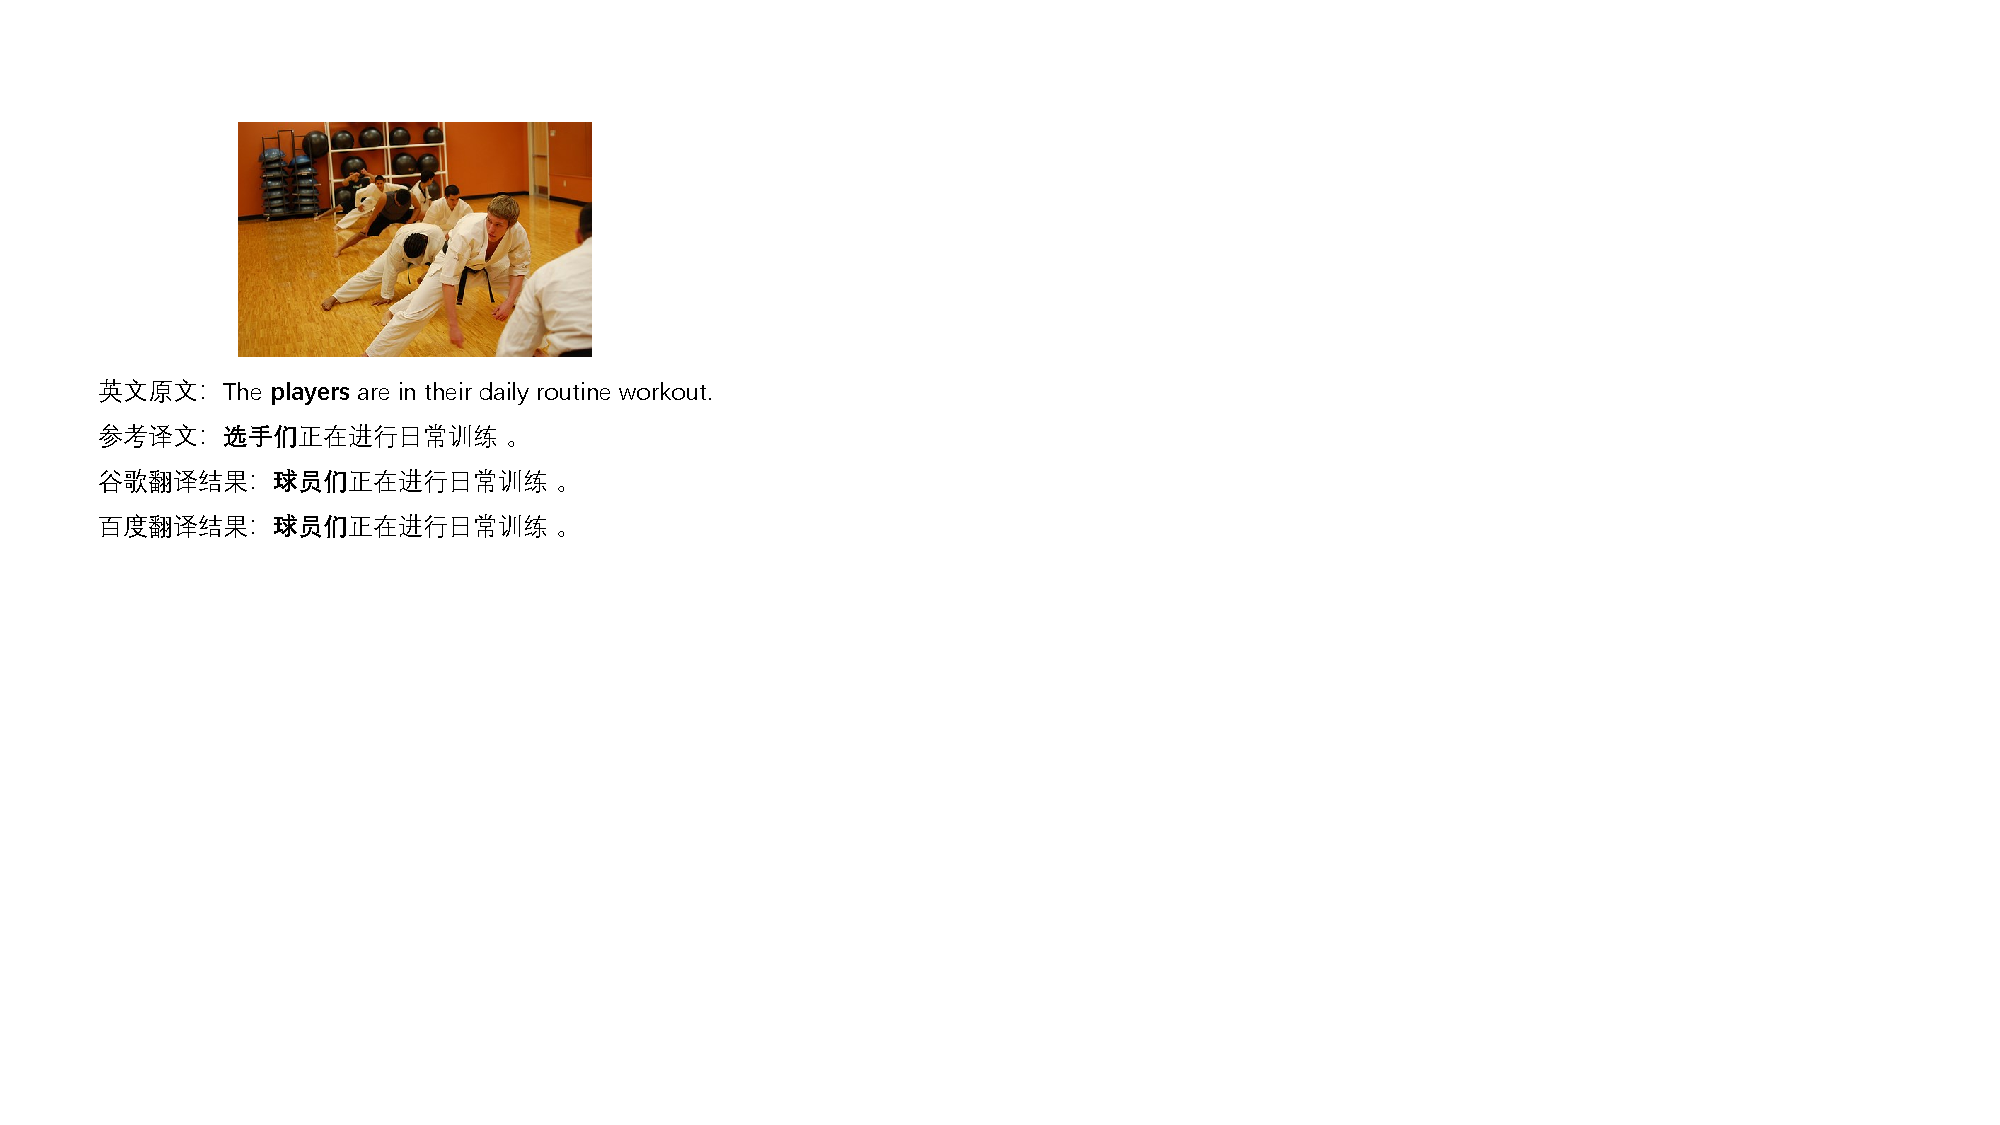
\includegraphics{Img/fig_1_case_players.pdf}
      \caption{错翻单词“players”}
      \label{fig:1_players}
    \end{subfigure}%
    \\
    \begin{subfigure}[b]{\linewidth}
      \centering
      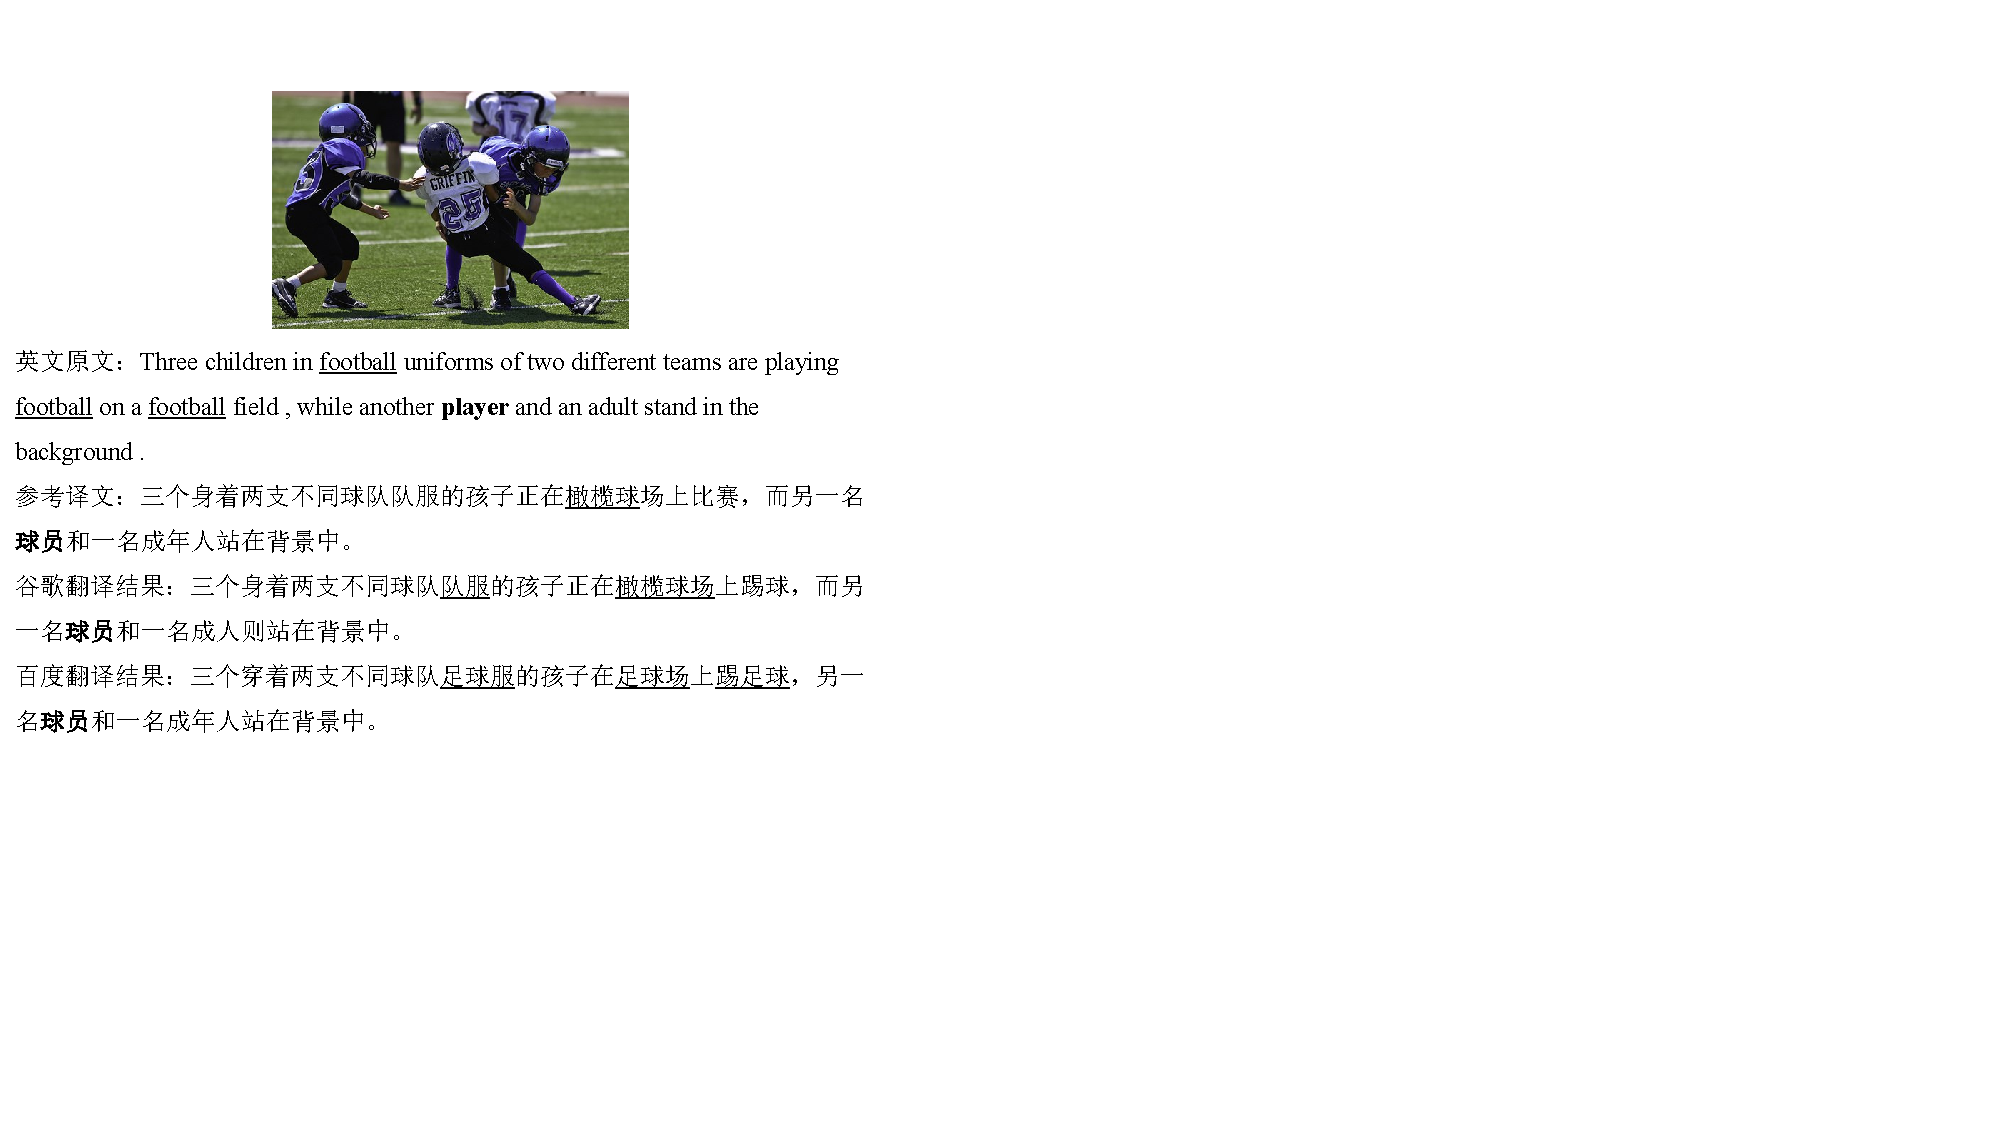
\includegraphics{Img/fig_1_case_football.pdf}
      \caption{错翻单词“football”}
      \label{fig:1_football}
    \end{subfigure}
    \bicaption{翻译错误案例}{Cases of incorrect translation}
    \label{fig:1_translation_cases}
\end{figure}
图\ref{fig:1_translation_cases}给出了谷歌和百度的机器翻译系统对两句英文图片描述的翻译结果。
在图\ref{fig:1_players}中展示了一个简单却缺少上下文信息的翻译例子,加粗项“players”在实际应用中随着背景信息的变化可以有多种不同的释义,在图例中应指的是“空手道选手们”。然而,在不考虑图片所提供信息的情况下,两个纯文本机器翻译系统均将其翻译为更常见的释义“球员们”。仅从文本的角度考虑,该翻译结果并不差,但因为文本所提供的信息是不完整的导致其翻译结果与真实释义存在一定的差距。
图\ref{fig:1_football}的例子中同时包含了“football”(下划线项)和“player”(加粗项)两个容易翻译错误的地方。从谷歌和百度翻译系统的结果中可以看到,在不提供图片信息的情况下,谷歌翻译系统将“football”翻译为“橄榄球”,而百度翻译系统将其翻译为“足球”。在未提供图片信息的情况下,不同的翻译系统表现出了不同的倾向性,仅从文本信息的角度两者都是正确的翻译。在图\ref{fig:1_football}的例子中“player”翻译到了正确的“球员”释义。其原因可以归结为两点,一是如同图\ref{fig:1_players}的例子一样,翻译系统选择了更为常用的“球员”释义;二是翻译系统捕捉到了整段原文中提供的有关于“球”的上下文信息,从而得到了正确的翻译。


上述例子表明,当句子中存在多义词、歧义词、语义不完整等问题时,图片中所包含的视觉信息能够作为翻译过程中所需要的上下文信息,而常规的神经机器翻译系统不具备建模和利用来自其它模态的信息的能力。在真实的应用场景中,翻译系统要处理的可能是商品介绍、聊天记录、网络简讯等有匹配图文的句子。因此,探索融合图片信息的神经机器翻译方法具有重要的理论研究和实际应用价值。图片中包含着更丰富、更完整以及更准确的信息能够为句子的翻译提供更适合的上下文语境,帮助模型得到优化的编码表示,或是为模型解码提供视觉信息作为参考。

相比于统计机器翻译,在神经机器翻译中融合来自图片中的信息是更方便且更自然的,这也推动了ImgNMT的研究热潮,相关研究大量涌现。目前的ImgNMT方法主要关注针对图片描述的翻译中,如何利用图片信息改进翻译质量。图片描述的翻译任务中,句子与图片具备语义上的一致性,图片与句子之间语义融合的研究可以从更多的角度展开,其相关研究成果与结论也可以更方便的应用到其它领域。相关的模型方法主要关注图片信息在神经机器翻译模型中的利用,提出了各具特点的网络结构以及采用各种图片输入方式来建模视觉上下文信息,从而方便图片信息在神经机器翻译模型中的利用。然而,神经网络方法为跨模态信息融合带来便利的同时,也极大地削弱了各种模型方法的可解释性。存在大量的方法对翻译质量的提升有限,但却因为图片信息作用方式不明确的原因,难以进行针对性的改进。另外,NMT所采用的平行翻译数据一般具有良好的语义对齐特性。相比之下,句子与图片之间的语义对齐关系则更为复杂。这使得一般的ImgNMT模型在训练阶段很容易收敛为一个忽略了图片信息的纯文本翻译模型,导致模型在应用测试阶段也仅是将输入的图片输入作为噪声。
因此,本文主要从模型层面出发,针对目前融合图片信息的神经机器翻译方法利用图片信息方式的缺陷,探索更有效的跨模态信息融合方法,从而提升神经机器翻译的译文质量。


\section{研究内容}

本文的研究旨在改善目前融合图片信息的神经机器翻译方法中图片信息的作用方式,提升图片与文本在语义融合过程中的作用程度,从而达到提升译文质量的目的。本文的研究内容主要包括:如何将图片信息明确地作用在句子中的对应目标;如何进一步改进明确的视觉信息作用方式,将其与常规的跨模态信息融合方法相结合;如何提升常规跨模态信息融合方法中图片信息的作用程度,利用更多的视觉信息改善翻译质量。

具体地,本文的主要工作可以划分为以下三个部分:

{\sffamily 1. 基于跨模态文本重构的神经机器翻译方法}

% 面对什么问题
主流的融合图片信息的神经机器翻译方法将图片输入到经过特殊设计的翻译模型中,利用神经网络方法具有直接从数据中学习数据特征的优点,实现将图片信息融合到句子的翻译中。但这种方法并不能保证图片在模型中的有效性,部分方法甚至不会为模型带来性能的提升。并且,图片信息的作用方式不明确,导致难以对方法实施针对性的改进。
%将图片输入到神经机器翻译模型中具有直接从数据中学习并融合跨模态信息的优点,但也难以明确图片信息的具体作用,因此这类方法可称为隐式跨模态信息融合法。
% 如何解决
为了探究显式跨模态信息融合法是否可行,本文提出一种基于跨模态文本重构的神经机器翻译方法。
% 具体怎么做
该方法将一个文本重构任务与翻译任务相结合,将文本重构任务作为辅助任务来提升翻译性能。在训练过程中,该方法首先使用视觉目标来替换源语言句子中与图片相关的部分,然后使用一个端到端生成式模型来恢复原始句子或生成目标语言句子。然后采用了参数共享机制,使得生成式模型在两个任务之间共享编码器或解码器部分,从而实现了对翻译模型的有效增强。
%该方法将一个文本重构任务与翻译任务相结合。文本重构模型在训练中将源语言句子中的名词或短语的位置明确地替换为图片中对应的视觉目标,并将该序列输入并重构到完整的源语言句子或目标语言的句子。由于文本重构模型也是端到端的文本生成式模型,因此可以通过参数共享的方式将重构模型编码器或解码器的参数与翻译模型共享,最终达到增强翻译模型的目的。
% 实验效果
实验表明,本文所提出的文本重构方法在测试阶段不需要输入图片的情况下有效地提升了模型的性能。并且该方法能够明确视觉信息为实体词的翻译带来了提升。

{\sffamily 2. 基于双向跨模态实体重构的神经机器翻译方法}

%面对问题
显式跨模态信息融合法能够将视觉信息明确地作用在词级或短语级的跨模态信息融合中。隐式跨模态信息融合方法主要作用在句子级别的语义融合。仅采用文本重构方法一方面只应用了图像到文本单方向重构,另一方面视觉信息仅作用到了实体词上,可以进一步增加句子级别的语义融合。
%如何解决
为了将显示跨模态信息融合方法与隐式方法相结合,本文提出一种基于双向跨模态实体重构的神经机器翻译方法,并将其与文本非实体重构方法相结合。
%具体做法
为了避免在重构过程中产生冗余信息,本文提出了一种新颖的跨模态信息融合方法,它放弃了对整个源语言句子的重构,而只针对实体和非实体进行不同类型的重构。实体重构代表着从文本实体中重构视觉实体和从视觉实体中重构文本实体的双向重构。文本非实体重构代表从文本上下文和视觉实体所组成的跨模态上下文中重构文本非实体。将双向重构与文本非实体重构三个任务和翻译任务融合为一个多任务学习框架,并提升翻译模型的性能。
%文本重构方法在重构的过程中生成了源语言端已经提供的信息。因此本文所提方法抛弃了文本级别的重构,在文本实体和视觉实体之间做双向的实体级重构。并增加了非实体的重构,使图片信息与文本上下文做进一步的信息融合。然后,将以上三种重构任务与翻译任务通过多任务学习的方式结合。
%实验结果
实验表明,该方法进一步地提升了机器翻译的质量。实验分析表明,双向实体重构与非实体重构的多任务组合方式使模型受益最大,说明显式方法与隐式方法的结合是有效的。

{\sffamily 3. 基于图文对比对抗训练的神经机器翻译方法}

%面对的问题
前两部分工作采用了图片增强式的神经机器翻译方法,利用多任务参数共享机制,将显示和隐式跨模态信息融合方法学习到的图片信息作用到翻译模型的参数优化中。但此类方法存在图片信息利用不充分的问题。将图片输入到翻译模型中的图片信息辅助式的神经机器翻译方法能够解决这个问题,但这类方法普遍存在模型对视觉信息不敏感的问题。
%如何解决
针对此问题,本文提出一种基于图文对比对抗训练的神经机器翻译方法。
%具体做法
为了增强模型对图片信息的利用,需要在模型训练过程增加一个图文语义匹配的功能。为此采用了对比学习方法,拉近翻译模型的图文对与译文在文本表示空间中的语义关系。然后再向负样本集中加入对抗样本。该对抗样本是将原图文对中的图片用随机的错误图片替换,使原文同时出现在正负样本集中。但因为输入的图片不一致,模型在对比学习的训练过程中需要将图片信息融合到文本表示中才能判断样本的正负性,并以此达到融合图片信息的目的。
%为了拉近双语的语义关系,在编码端增加了图文与目标语言句子之间对比学习。并在负样本集中引入了包含源语言句子+错误图片对抗样本。为了将正负样本区分开,模型需要判断图片信息是否与源语言句子的语义一致。该方法会将图片信息融合到文本的表示中,从而提升视觉信息在模型中的作用程度。
%实验结果
实验结果表明,该方法提升模型翻译性能的同时还提升了模型对视觉信息的敏感度,输入正确图片的翻译结果明显优于输入错误或不输入图片的情况。


\section{论文的组织结构}

围绕上述研究内容,本文共分为六章,具体的组织方式如下:

第1章为绪论部分。本章首先机器翻译以及融合图片信息的神经机器翻译的研究背景和意义进行介绍,并指出神经机器翻译方法在融合图片信息的过程中存在哪些问题,随后介绍了本文针对目前存在问题所做的研究内容,最后在本节介绍了论文的组织结构。

第2章为融合图片信息的神经机器翻译方法国内外研究现状。本章首先详细介绍了神经机器翻译模型的发展历程和基础的模型框架。然后介绍了在将图片信息传递给神经机器翻译模型前,有哪些计算机视觉基础模型可以为跨模态信息的融合提供便利。紧接着,对融合图片信息的神经机器翻译方法进行了分类介绍,包括图片信息辅助式方法、图片信息增强式方法、基于图片搜索的方法以及无监督方法。最后,分析了现有方法所面临的问题与挑战,进而引出本文所要开展的工作。

第3章介绍了基于跨模态文本重构的神经机器翻译方法。为了将图片信息明确地作用到文本中的对应目标上,本章首先介绍了图片中的视觉目标与文本中的词或短语的对齐方法,设计了图片目标在文本编码过程中的明确作用方式。然后设计了两种文本重构方案和三种参数共享方案将重构任务融合到文本翻译任务中。最后介绍了所提方法在英德翻译数据上的实验结果。

第4章介绍了基于双向跨模态实体重构的神经机器翻译方法。为了进一步挖掘采用明确方式融合图片信息方法的潜能,本章首先介绍了文本实体到图片实体和图片实体到文本实体两个方向的实体级重构方案。为了充分利用图片中的视觉信息,将视觉信息与文本上下文融合,本章还介绍了非实体的重构方案。然后将以上三种重构方法以多任务学习的方式与翻译任务相结合。最后介绍了此多任务方法在三个翻译对上的有效性。

第5章介绍了基于图文对比对抗训练的神经机器翻译方法。为了在图片与文本信息融合过程中,使模型对图片中所包含的信息更敏感,本章首先介绍了一种在对比学习中加入对抗样本作为负样本的方法。然后在多个语言对上测试了所提方法提升翻译准确率的能力。最后分析了,对比对抗训练方法能否提升图片在神经机器翻译中的作用。

第6章对本文的研究工作进行总结,分析现有研究工作的不足,并对未来的研究工作进行展望。
\chapter{研究现状综述}\label{chap:relatedwork}

% 2.1 引言
\section{引言}
% 任务背景
% 可以介绍统计机器翻译到神经机器翻译的变革,带来了哪些影响,例如在多模态融合等方面的影响
机器翻译是一种利用计算机算法将一种语言翻译到另一种语言的技术。从统计机器翻译时代,到神经机器翻译时代,机器翻译相关技术一直作为行业的风向标引领着整个自然语言处理领域的发展。其基础模型从做到打破语言壁垒突破至跨越模态整合,能够在计算机视觉、语音信号处理以及多模态信息融合等领域都得到广泛的应用。
% 任务起源
% 可以提到机器翻译的缺陷,比如歧义、信息不充足等问题试图通过外源信息来解决
多模态机器翻译就是一种在机器翻译的基础上,融合图像信息、语音信息或者视频信息的一类方法。这些引入的外源信息,在理论上具有解决歧义词、转录错误以及语义不完整等问题的意义。

% 任务形式
% 讲讲与机器翻译的区别、如何将其分为了两大类。
融合图片信息的神经机器翻译是多模态神经机器翻译方法的一个分支,是一种将图片作为外源辅助信息输入到神经机器翻译模型中,以提升翻译准确率为目的的方法。因此,与常规的神经机器翻译相似的是,相关研究所使用的语料同样需要平行翻译句对的形式,区别在于增加了与文本内容高度相关的图片输入。根据图片信息的作用方式,可以将相关方法分为图片信息辅助式、图片信息增强式、图片搜索式以及无监督式的四类方法。本章首先将简要介绍神经机器翻译的发展过程,以及用于对图片进行预处理以及特征提取的计算机视觉基础模型,然后按照图片信息辅助式、图片信息增强式、图片搜索式和无监督式的方法分类,分别介绍融合图片信息的神经机器翻译如何随着神经机器翻译的发展而进行改进。

% 2.2 神经机器翻译
\section{神经机器翻译模型}
\label{sec:2_nmt}
在融合图片信息的神经机器翻译中,平行翻译句对的源语言句子与目标语言句子之间一般具有很强的语义对齐关系,而图片主要起到补充信息的作用。因此,ImgNMT所使用的模型多数是以神经机器翻译模型作为基础框架,视觉特征作为模型的额外输入。本节将介绍ImgNMT在模型设计发展过程中所应用到的神经机器翻译基础模型框架,这其中包含:基于循环神经网络(recurrent neural network,RNN)方法的神经机器翻译(RNN-based neural machine translation,RNMT)模型\pcite{sutskever2014sequence,cho2014learning}、增加注意力机制的RNMT模型\pcite{bahdanau2015neural,luong2015effective}以及基于自注意力机制的Transformer\pcite{vaswani2017attention}。另外,还有基于卷积神经网络(convolutional neural networks,CNN)的NMT模型\pcite{gehring2017convolutional},但其很快被自注意力机制取代,也没有在ImgNMT任务上得到应用,因此本节忽略这部分内容的介绍。

\subsection{循环神经网络}
\label{sec:2_rnn}
\input{Tex/2_RelatedWork/figure_rnmt}
神经机器翻译是一种序列到序列的生成任务,其源端序列与目标端序列的长度往往是不同的。因此,编码器-解码器结构成为了神经机器翻译的常用模型框架。编码器和解码器分别用于编码源端序列和解码到目标端序列。循环神经网络就是一种用于解决序列建模的方法。图\ref{fig:2_rnmt}为基于循环神经网络的神经机器翻译框架。编码器将不定长的源语言句子编码为单个固定维度的隐层向量,该隐层向量可作为整个句子语义的特征表示。解码器负责根据该特征表示生成目标语言句子。形式化地,给定待翻译的源语言句子$X=\{x_1,x_2,…,x_N\}$,在编码端首先需要将$X$中的词转化为词向量$E=\{\Vector{e_1,e_2,…,e_n}\}$,其中:
\begin{equation}
    \Vector{e_i}=\mathrm{Emb}(x_i)
\end{equation}

源语言句子中的每个词$x_i$均有一个对应的词向量表示$\Vector{e_i}$。然后编码器按照句子中词的顺序将句子编码到一个隐层状态序列$\rarwvec{H}={\rarwvec{h}_1,\rarwvec{h}_2,…,\rarwvec{h}_N}$,其中,$\rarwvec{h}_i$中编码了输入序列中前$i$项的信息,即:
\begin{equation}
    \rarwvec{h}_i=\mathrm{RNN}(\rarwvec{h}_{i-1},\rarwvec{e}_i)
\end{equation}
其中$\rarwvec{h}_{0}$可随机初始化或置为零向量。为了使每个位置的编码都能融合整个输入序列的信息,可采用双向编码器将句子$X$同时编码到$\rarwvec{H}$和$\larwvec{H}$,其中,$\larwvec{H}=\{\larwvec{h}_1,\larwvec{h}_2,…,\larwvec{h}_N\}$为$X$的逆序编码结果,即:
\begin{equation}
    \larwvec{h}_i=\mathrm{RNN}(\larwvec{h}_{i+1},\larwvec{e}_i)
\end{equation}
将$\rarwvec{H}$和$\larwvec{H}$拼接得到$\Vector{H=\{h_1,h_2,\cdots,h_N}\}$, 其中:
\begin{equation}
    \Vector{h_i}=[\rarwvec{h}_i;\larwvec{h}_i]
\end{equation}

RNMT的解码器同样采用循环神经网络生成目标语言文本。该生成翻译的过程是自回归的,即在时刻$t$,解码器需要根据$0$至$t-1$时刻的解码结果及源语言所提供的上下文信息进行当前时刻的预测结果的生成:
\begin{equation}
    \Vector{s}_t=\mathrm{RNN}(\Vector{s_{t-1}},y_{t-1})
\end{equation}
\begin{equation}
    P(y_t|y_{<t},X)=\mathrm{softmax}(g(\Vector{s_t}, y_{t-1}, \Vector{c_t}))
\end{equation}
该过程中,源端上下文信息的作用方式有很多种。\tcite{sutskever2014sequence}将$\rarwvec{h}_N$传递给解码器作为初始状态$\Vector{s_0}$。\tcite{cho2014learning}将$0$至$t-1$时刻的解码结果编码,并连同源端上下文信息$\Vector{H}$预测当前时刻单词:
\begin{equation}
    \Vector{c_t}=f(\Vector{H})
\end{equation}
其中,$f(\cdot)$表示选用平均池化(average pooling)对$\Vector{H}$取平均,或直接选取$\Vector{H}$的最后一项$\Vector{h_n}$。

虽然基于循环神经网络的神经机器翻译还没有实现对传统统计机器翻译在翻译准确率上的全面超越,但其采用的编码器-解码器框架已经展现了能够将文本数据进行分布式表示并从这种表示中解码到目标语言译文的能力。这种分布式表示方法也为跨模态信息的融合提供了极大的便利。

\subsection{注意力机制}
\label{sec:2_attention}
基于编码器-解码器结构的神经翻译模型利用编码器将源语言编码为一个固定的特征向量,再利用解码器中的循环神经网络编码已生成的目标端单词,从而指导新的目标端单词的生成。在该过程中,编码的源语言特征向量作为句子级语义的完整表示,一方面丢失了源语言中的句长信息,另一方面无法指导在当前时刻$t$生成目标端单词时应该更多地关注源端的哪些信息。为了解决这个问题,\tcite{bahdanau2015neural}提出在编码器与解码器之间增加注意力机制(attention mechanism)。

\input{Tex/2_RelatedWork/figure_att_rnmt}
图\ref{fig:2_att_rnmt}为增加了注意力机制的神经机器翻译,其编码器和解码器保留原来的工作方式,而两者之间的注意力模块为解码器提供了动态的源语言上下文信息。对于每个时刻$t$,源语言上下文向量$\Vector{c_t}$由固定的特征向量替换为与$t$相关的表示:
\begin{equation}
    \Vector{c_t} = f_t(\Vector{H})=\sum_{i=1}^{N}{\alpha}_{ti}\Vector{h_i}
\end{equation}
\begin{equation}
    {\alpha}_{ti}=\frac{\mathrm{exp}(a_{ti})}{\sum_{j=1}^{n}\mathrm{exp}(a_{tj})}
\end{equation}
\tcite{bahdanau2015neural}所提方法中:
\begin{equation}
    a_{ti} = \mathrm{score}(\Vector{s_{t-1},h_i})
\end{equation}
其中$\mathrm{score}(\cdot)$是打分函数,计算两个向量所携带信息的相关程度,可采用点积或多层感知机等方法。上式对$\Vector{s_{t-1}}$和$\Vector{h_i}$进行打分,表示根据已生成的目标文本编码表示$\Vector{s_{t-1}}$,计算源语言中第$i$项对当前时刻$t$的重要程度。因此,$a_{ti}$代表着生成$t$时刻的目标端单词时,对源语言中第$i$项的“关注”度,${\alpha}_{ti}$就是该“关注”度的归一化结果,$\Vector{c_t}$就是根据“关注”度对特征向量的加权表示。

值得注意的是,$t-1$时刻的输出结果$y_{t-1}$是由$\Vector{s_{t-1}}$得到的,因此上式中丢失了$y_{t-1}$的信息,\tcite{luong2015effective}提出了改进方案:
\begin{equation}
    a_{ti} = \mathrm{score}(\Vector{s_{t},h_i})
\end{equation}
并规定了$\mathrm{score}(\cdot)$的三种计算方式,综合\tcite{bahdanau2015neural}等提出的方法,可得到以下四种方法:
\begin{equation}
    \mathrm{score}(\Vector{s_t, h_i}) = 
    \begin{cases}
        \Vector{s_t^T h_i} & \mbox{{\itshape 点积法}} \\
        \Vector{s_t^T W_a h_i} & \mbox{{\itshape 通用点积法}} \\
        \Vector{W_a[s_t; h_i]} & \mbox{{\itshape 连接法}} \\
        \Vector{v_a^T} \mathrm{tanh}(\Vector{W_a s_t+U_a h_i}) & \mbox{{\itshape 多层感知机法}} 
    \end{cases}
\end{equation}
其中$\Vector{v_a}$、$\Vector{W_a}$和$\Vector{U_a}$是网络参数,$T$表示对向量进行转置。

%(注意力机制在视觉领域的应用,以及在跨模态领域的应用。)

\subsection{Transformer}
\label{sec:2_transformer}
\input{Tex/2_RelatedWork/figure_transformer}
在注意力机制的帮助下,基于循环神经网络的神经机器翻译得到了显著的性能提升。这说明基于动态上下文的解码方法能够更准确地捕捉上下文信息,从而得到更忠于原文的译文。而注意力机制相当于二次编码,为下游模块提供动态上下文。既然注意力机制同样具有编码能力,那么是否可以用于替换循环神经网络呢?谷歌提出的Transformer\pcite{vaswani2017attention}就是一种基于这种假设的模型。图\ref{fig:2_transformer}展示了Transformer的模型结构,其保留了编码器-解码器的基础框架,利用内置的多头注意力机制(multi-head attention mechanism)实现编码与解码过程。


\input{Tex/2_RelatedWork/figure_multihead}
区别于一般的注意力机制,多头注意力机制采用了一种更具泛化性的模型设计。如图\ref{fig:2_multihead}所示,多头注意力机制的输入分为查询(query,Q)、键(key,K)以及值(value,V)三部分,并结合了缩放点积注意力(scaled dot-product attention)和多头注意力(multi-head attention)两种方法。

{\sffamily 缩放点积注意力:}与一般的点积法相比,缩放点积注意力增加了一个缩放因子$d_k^{-0.5}$:
\begin{equation}
    \mathrm{Attention}(\Vector{Q},\Vector{K},\Vector{V}) = \mathrm{softmax} \left( \frac{\Vector{Q}\Vector{K}^T}{\sqrt{d_k}} \right) \Vector{V}
\end{equation}
其中,$d_k$代表$\Vector{Q}$、$\Vector{K}$和$\Vector{V}$的隐层维度。采用点积法的优点在于点积是以矩阵乘的形式进行计算,通过底层代码优化等方法可以很好地对矩阵乘进行硬件加速。引入缩放因子则是为了防止$d_k$较大时,点积的数值膨胀导致$\mathrm{softmax}(\cdot)$函数逼近梯度消失的数值范围。

{\sffamily 多头注意力:}为了丰富动态上下文所承载的信息,\tcite{vaswani2017attention}将多个注意力模块拼接组成多头注意力机制:
\begin{equation}
    \mathrm{MultiHead}(\Vector{Q,K,V}) = \mathrm{Concat}(\Vector{head_1, \cdots, head_n})\Vector{W^O}
\end{equation}
\begin{equation}
    \Vector{head_i} = \mathrm{Attention}(\Vector{Q W_i^Q,K W_i^K,V W_i^V})
\end{equation}
其中,$\Vector{W_O}$,$\Vector{W_i^Q}$,$\Vector{W_i^K}$和$\Vector{W_i^V}$是模型参数。$\Vector{Q}$、$\Vector{K}$和$\Vector{V}$经过不同的参数映射到不同的表示空间,再由注意力机制编码得到的不同的上下文特征表示。该过程相当于在不增加额外参数的情况下,将多个模型集成到一个模型中,从而提升模型的学习能力。

多头注意力机制在Transformer中的用途分为三种:
\begin{itemize}
    \item 位于编码器的多头自注意力机制用于编码源语言句子,此时Transformer编码器第一层的$\Vector{Q}$、$\Vector{K}$和$\Vector{V}$均为源语言句子经映射后的词向量序列,其它层的$\Vector{Q}$、$\Vector{K}$和$\Vector{V}$为前一层的输出。
    \item 位于解码器中带有掩码的多头自注意力机制用于编码目标端已经解码出来的部分句子。掩码的作用是为了保持自回归解码过程中后面位置单词的解码只能用到前面位置信息的特性。
    \item 连接编码器与解码器的多头交叉注意力机制的作用和一般的注意力机制相似。此时$\Vector{Q}$为解码器中带有掩码的多头自注意力机制的输出,$\Vector{K}$和$\Vector{V}$为编码器的隐层输出。交叉注意力机制输出的是融合了源端信息的目标端句子的表示。
\end{itemize}

值得注意的是,基于注意力机制的编码过程与循环神经网络相比丢失了对输入序列位置信息的建模。因此,\tcite{vaswani2017attention}提出了位置编码(positional encoding),为每个词向量增加位置信息。%文献\cite{DBLP:journals/corr/GehringAGYD17}则提出了更为方便的位置词向量的方案。

尽管近年来针对Transformer框架的改动层出不穷,但广泛应用的模型基本保持了最原始的设计方案。常见的改动如\tcite{devlin2019bert}提出了使用位置词向量(positional embedding)的方式替换位置编码,以及为了加强Transformer对长序列的编码能力提出相对位置编码\pcite{shaw2018self,dai2019transformerxl}。而这些创新性的改动基本都保留了Transformer中的自注意力机制和交叉注意力机制的基本结构。除了机器翻译等生成式任务外,在大规模预训练任务的表现上,Transformer更是充分展现了其应用场景的灵活性\citep{radfordimproving,devlin2019bert,liu2019roberta,lewis2020bart,raffel2020exploring}。针对不同规模的数据,通过增减参数规模的方式就可以使其适应相应的任务。相比于基于循环神经网络的模型,Transformer能够容纳更长的输入序列和更大规模的网络参数。

Transformer出色的编码能力不仅在自然语言处理任务大放异彩,还在计算机视觉以及多模态信息融合等领域展现了不俗的潜能。例如在计算机视觉领域的图像分类、目标检测以及语义分割等传统任务上摒弃了基于卷积神经网络的方法,直接采用Transformer作为基础模型,并在多个任务上得到了进一步的性能提升\pcite{parmar2018image,dosovitskiy2021vit,liu2021swin,yuan2021tokens};或是在大规模文本预训练模型的基础上,在输入序列中增加图片输入或从图片中提取的视觉目标,提升Transformer在多模态自然语言理解(multi-modal natural language understanding)任务上的能力\pcite{lu2019vilbert,chen2020uniter,huang2020pixelbert,kim2021vilt}。

%(Transformer已经在业界产生的影响力,自注意力替换循环神经网络的必要性,解决了哪些问题)

% 2.3 visual backbones
\section{计算机视觉基础模型}
\label{sec:2_cv}

深度学习技术不仅推动着自然语言处理技术的发展与革命,其在早期更是在计算机视觉领域推动各项技术从研究起步迈向成熟落地。相比于自然语言处理技术在近年来才迎来应用热潮,计算机视觉中的相关研究则早已应用到生产生活中。这也是目前大部分融合视觉信息的自然语言处理任务均应用预训练好的计算机视觉基础模型对图像进行编码的原因。

融合图片信息的神经机器翻译任务需要将图片信息输入到神经机器翻译模型中,因此同样需要采用神经网络方法对图片信息编码。针对不同的翻译模型选择合适的图片编码方法,能够提升视觉信息在翻译模型中的作用,从而帮助提升翻译模型的性能。目前ImgNMT中融合图片信息的方式主要可以分为三类:图片全局信息、图片动态局部信息以及视觉目标信息。本节将主要针对这三类图片信息作用方式介绍其背后的计算机视觉基础模型。

% 基础模型在ImgNMT中的利用:
%   CNN:全局特征、栅格特征
%   R-CNN:视觉目标特征
%   visual grounding:(短语,视觉目标特征)

\subsection{卷积神经网络}
\label{sec:2_cnn}

卷积神经网络是目前计算机视觉领域最重要且最流行的方法之一,可以在计算机视觉的多个研究任务中发挥重要作用,例如图像分类、目标检测、人脸识别、语义分割等。早在20世纪90年代,杨·乐坤(Yann LeCun)等人发表论文提出了LeNet-5,成为奠定了现代卷积神经网络方法的基础框架\pcite{fukushima1980neocognitron,lecun1989handwritten,lecun1998gradient}。
现有的卷积神经网络,如AlexNet\pcite{krizhevsky2012imagenet},VGGNet\pcite{simonyan2015very},GoogLeNet\pcite{szegedy2014going},ResNet\pcite{he2016deep},DenseNet\pcite{huang2017densely}等模型,均是在LeNet-5的基础上进行的改进。%通过加深网络层数、增加或改变非线性激活层、增加批数据归一化、增加通道数量等手段提升网络的泛化性能和增强对图像的表征能力。
卷积神经网络不仅在计算机视觉领域得到广泛应用,在语音识别和自然语言处理的某些特定任务上同样得到了关注。在融合图像信息的多模态任务上,卷积神经网络更是用于表征图片信息或视频信息的必然选择。本节将以LeNet-5为例,简要介绍卷积神经网络的基本结构,以及应用到跨模态信息融合时的使用方式。

\input{Tex/2_RelatedWork/figure_lenet5}
LeNet-5是最早的卷积神经网络模型之一,设计之初被用于手写数字识别任务。图\ref{fig:2_lenet5}展示了LeNet-5从输入图片到输出预测结果的模型工作简化图。LeNet-5共包含5层,包括两个卷积层(convolutional layer)C1、C3、C5,以及两个池化层(pooling layer)S2和S4。

{\sffamily 卷积层:}卷积层是CNN模型的核心模块,包含了整个模型的大部分参数。它可以对输入图像的局部区域进行加权求和从而得到图片的特征(feature)或特征图(feature map,FM),例如示例中经过卷积层得到的特征或特征图有FM1、FM3和F5。卷积层中卷积核(convolution kernel)大小和形状的选择能够影响卷积的效果。例如,图\ref{fig:2_lenet5}中卷积层C1中有6个$5 \times 5 \times 1$的卷积核,每个卷积核将图片中每个$5 \times 5$大小区域内的像素点加权求和得到输出特征图中的一个像素点,因此一个$32 \times 32$大小的图片经过卷积层C1后得到的特征图FM1的大小为$6 \times 28 \times 28$。经过卷积层后,图片的通道数可能会增加,图片的尺寸也可能变小。卷积层的设计可以很简单也可以非常的复杂,例如卷积层C3中包含了16个卷积核,其中各卷积核的尺寸为$5 \times 5$,但选取的特征图数量(图中包含6,4,3三种数量的差别)却各不相同。这说明卷积层的设计可以是非常灵活的,也因此对模型设计与研究人员的考验也是巨大的。

{\sffamily 池化层:}池化层一般也称为下采样层(subsampling layer),相当于一个过滤器,对图片或特征图执行降维操作,滤掉无用的像素点,帮助模型提取更高层次的特征。其原理是在输入特征图中一个局部区域内,按照选取最大值或计算平均值的方式为输出特征图增加一个新的像素点,也称最大池化(max pooling)和平均池化(average pooling)。例如图\ref{fig:2_lenet5}中的池化层S2的大小为$2 \times 2$,它在图片中对应区域内选取最大值或计算平均值后输出到特征图FM2中。区别于卷积层,池化层对输入特征图进行过滤像素时,一般不设置重叠区域,例如图中的池化层的尺寸和步长均为2,因此特征图经过池化层后特征图的尺寸变为原来的二分之一。

{\sffamily 全连接层:}全连接层(full connection layer)层中的每个神经元都连接着上一层的所有神经元。区别于卷积层和池化层将图片映射到隐层的特征空间中,全连接层将隐层表示映射为图片的分布式特征表示,或经过非线性激活函数(一般采用softmax函数)得到样本的概率模型并预测样本的分类结果。例如图\ref{fig:2_lenet5}中最后的全连接层将图片特征F6映射为一个维度为10的向量中,每个维度的取值为0到1,代表着预测为0到9每个值的概率。

虽然LeNet-5的结构简单,但依旧展现了卷积神经网络能够学习并表征图片信息的能力。层数更深,网络结构更复杂,以及采用了更多新技术的新一代卷积神经网络能够表征更复杂的图像信息。在融合视觉信息的自然语言处理任务中,因文本输入与图片输入很难在一个模型中同时支持,因此通常采用特征融合的方式支持多模态输入。从一般的卷积神经网络的模型结构可以看到,选取图片特征的选择可以有很多种。例如图\ref{fig:2_lenet5}中FM4的尺寸为$16 \times 5 \times 5$,其中,在$5 \times 5$的特征图内仍保留着与源图片中的区域对应关系。因此FM4可看作是由$5 \times 5$个维度为16的特征组合而成,每个16维的特征表征了图片中对应的区域。这种保留了图片内局部空间信息的特征图一般称为栅格特征(grid feature)或局部特征(local feature)。在融合图片信息的神经机器翻译方法中,栅格特征一般可以作为图片输入序列输入到翻译模型中,通过注意力机制能够动态地关注到栅格特征中保留的局部空间信息。利用平均池化将栅格特征所代表的多个视觉特征融合为一个视觉特征,称作全局特征(global feature)。全局特征表征了图片的全局信息,通常可以用于初始化循环神经网络,或作为词向量等方式输入到神经机器翻译模型中。

% 要强调栅格信息保留了位置信息
% 这里最好直接举ResNet的例子,可以直接将残差连接的引入到现有机器翻译模型中

\subsection{目标检测方法}
\label{sec:2_object_detection}
%方法背景介绍
\input{Tex/2_RelatedWork/figure_visual_object_detection}
目标检测是计算机视觉领域中一个应用范围非常广的任务,其目的是在图像或视频中自动地定位并识别出特定的视觉目标,从而满足对视觉目标的筛选、分类、追踪等需求。早期的目标检测算法需要手工设计特征和分类器来实现物体检测,并且运行速度较慢。随着深度学习的发展,目标检测算法开始采用卷积神经网络作为基础模型实现对视觉目标的检测,并取得了很好的性能与速度。对于融合图片信息的神经机器翻译任务,目标检测同样是非常重要的应用手段之一。与卷积神经网络能够提供图片的全局特征和栅格特征相比,目标检测的结果能够直接将图片中最有价值的前景信息提供给翻译模型。并且,每个视觉目标都能够提供排除与视觉目标不相关的更集中的视觉信息。

根据各算法特点以及工作方式,可以将目前常用的目标检测算法可以分为三类:两阶段法、一阶段法、语义目标提取法(visual grounding)。其中两阶段法和一阶段法提取给定图片中的所有类别可知的目标,并将提取出的目标分到相应的类别。语义目标提取法是根据语义信息提取相应的视觉目标,因此可以与前两者区分开。

{\sffamily (1)两阶段法}

两阶段法的代表方法有R-CNN(region-based convolutional neural networks)\pcite{girshick2014rich}、Fast R-CNN\pcite{girshick2015fast}以及Faster R-CNN\pcite{ren2015faster},如图\ref{fig:2_object_detection}(a)。这类算法在目标检测过程中通常分为提取候选区域(region proposal)和特征提取与分类回归两个阶段。
从图片中提取视觉目标的最简单方式就是采用滑动窗口方法遍历图片中所有的矩形区域,然后利用分类器将有效的矩形区域分类到与其对应的类别。很显然,这种枚举的做法会消耗大量的检测时间。因此常见的两阶段法都会采用精心设计的算法提取出图片中的部分候选区域。
例如,在R-CNN中采取了选择性搜索(selective search)算法在原始图片中提取出1000至2000个候选区域,也称感兴趣区域(region of interest,RoI),这种做法的弊端就是需要对这些候选区域都进行一次CNN的编码,同样耗费很多时间。
而Fast RC-NN为了节省这部分时间先将图片经过CNN表征后再利用其所设计的RoI池化方法将栅格特征中与RoI相对应的区域提取出来。
为了更进一步地提高效率,Faster R-CNN方法采用了区域提取网络(region proposal network,RPN)代替耗时的选择性搜索算法。
通过第一阶段的提取就可以得到每个RoI的特征表示了。采用深度学习算法之前都是通过人工设计的特征来表征图片,而目前都是通过CNN来更方便的表征图像信息。将RoI的特征表示经过分类器就可以判断当前RoI是否属于某个已知的类别从而完成对提取到的视觉目标的分类。同时还要经过回归算法来获得目标的更精确的方框定位(bounding box)。

{\sffamily (2)一阶段法}

一阶段法的代表方法为YOLO(you only look once)\pcite{redmon2016you,redmon2017yolo9000,redmon2018yolov3,bochkovskiy2020yolov4,ge2021yolox}系列算法,其特点是采用单个神经网络同时完成对图像中视觉目标的提取和分类,而不需要预先生成候选区域。因此,一阶段法具有更快的目标检测速度。图\ref{fig:2_object_detection}(b)展示了YOLO算法的简化示意图,其基本工作原理是直接采用回归的方式替代预提取和分类的组合方式,利用CNN对图像的表征对图片中的方框坐标$(c,x_1,y_1,x_2,y_2)$进行回归,从而达到仅需要进行一次CNN的前向计算就能够得到检测结果的目的,其中$c$代表预测的置信度(confidence),$(x_1,y_1)$与$(x_2,y_2)$分别代表方框的左上角和右下角在图片中的位置坐标。为了能够一次提取图片中的多个视觉目标,则将输入图片划分为多个区域,每个区域负责一个视觉目标的提取。当视觉目标的中心落在某个区域时,该区域负责对该视觉目标的提取,例如图\ref{fig:2_object_detection}(b)中,图片被虚线分割的每个矩形区域与矩阵中每个位置一一对应,矩阵中“1”的位置分别对应了图片中“人”、“帽子”和“眼镜”的中心所在的矩形区域。

{\sffamily (3)语义目标提取法}

在图片中提取与文本语义相关区域的方法是语义目标提取法,方法示意图如图\ref{fig:2_object_detection}(c)所示。这类方法的输入是一张完整的图片和需要提取内容的文本。例如提取图片中的“人”时,其模型输入为图片和文本“人”、“男人”或者“一个戴眼镜的男人”。提取视觉目标的过程需要对图片和文本先编码,然后利用跨模态信息融合的方式识别出图片中与文本语义最相近的区域。最初的语义目标提取可以认为是目标检测任务的下游任务,所用的方法是先采用常用的目标检测方法将图中的视觉目标提取出来并分类。然后根据视觉目标类别与输入文本相似度通过匹配的方式完成语义目标的提取。这种传统的语义目标提取方法因为需要两种方法相结合才能完成任务,因此也称为两阶段法。而图\ref{fig:2_object_detection}(c)中所展示的方法不需要先提取再匹配的过程,所有提取步骤在一个统一的模型中完成,因此称为一阶段法。采用语义目标提取法获得视觉目标的方式能够将文本的内容与图片中的视觉目标对应起来,对于跨模态信息融合有很大的帮助。本文在后面的章节\ref{sec:3_entity_extraction}小节所介绍的工作就采用了一种一阶段的语义目标提取法,来获取句子中的短语与图片中的视觉目标的对应关系。
%方法介绍

%在ImgNMT中的应用

%对于跨模态信息融合,目标检测依旧是非常重要的应用手段之一。与卷积神经网络相比,目标检测的结果能够直接将图片中那些信息量最大的目标直接提供给翻译模型,而提取出的视觉目标所包含的信息也更集中。目标检测的结果可以分为两种,一种是检测结果与文本不建立关系,此时目标检测方法输出的多个视觉目标结果可以视为视觉目标序列输入到以序列建模擅长的自然语言处理任务的模型中。另一种是通过文本语义进行视觉目标检测,这种方式能够对齐文本与视觉目标,更方便在翻译中使用。
% 目标检测要给出区域,和分类
% 最初的设定,扫描图片中的所有框
% R-CNN:two-stage,ROI->feature extraction for ROI->SVM->位置精修
%      R-CNN-> Fast R-CNN -> Faster R-CNN
% Yolo v0-5: one-stage (you only look once)(regression)
%      v0: 遍历所有“框” -》 输出(c,x,y,w,h) 其中c为confidence,label为(1,x*,y*,w*,h*)
%      v1:检测多个目标,将img划分为多个区域,(c,x,y,w,h,one-hot)*N
% visual grounding

%\subsection{视觉Transformer}
%这里和前面呼应以下,前面是CV推动着NLP的发展,这里则反过来,NLP推动CV

%预示着大模型的融合

%与CNN相同同样可以做backbone,做目标检测以及图片分类

% 结尾说以下那几篇文章说过使用哪种CNN-backbone带来的差别并不大
% 2.4 MMT
\section{融合图片信息的神经机器翻译}
\label{sec:2_imgnmt}

%研究意义与背景介绍
得益于深度学习技术在自然语言理解和计算机视觉等领域的快速发展,融合文本与图片信息的跨模态理解与生成也成为了可能。融合图片信息的神经机器翻译就是将已经成熟的计算机视觉方法与神经机器翻译技术相结合的一类研究。其研究历程也紧随着纯文本神经机器翻译的脚步而发展。一个标准的神经机器翻译系统通常以句子为翻译单位。端到端的翻译模型通过拟合大量双语数据中语言之间的对齐特性习得翻译能力,在编码过程将源语言句子的信息编码为分布式的向量表示,再通过解码器将表示向量解码到目标语言。然而,针对翻译采集的数据也包含着人类语言应用中的使用习惯与问题。例如文本中存在多译词、歧义词或者不完整表达等问题,都需要通过待翻译句子以外的补充信息来解决,而图片中往往包含着更丰富、更完整以及更准确的信息。因此在翻译一个句子时,图片中的视觉信息能够其提供所需的外源补充信息。为此,研究者们提出了融合图片信息的神经机器翻译方法(image-incorporated neural machine translation,ImgNMT)。

% 任务定义
融合图片信息的神经机器翻译方法的目的是在基于神经机器翻译的框架内,借助图片信息生成更准确译文。该方法是多模态机器翻译(multi-modal machine translation)的一个研究子类。相关的多模态机器翻译还包含口语翻译\cite{82_DBLP:conf/icassp/Vidal97,83_DBLP:conf/icassp/Ney99,84_DBLP:conf/interspeech/WeissCJWC17,85_DBLP:conf/icassp/BerardBKP18}(spoken language translation,SLT)和视频引导翻译\cite{86_DBLP:conf/lrec/LisonT16,87_DBLP:journals/corr/abs-1811-00347,88_DBLP:conf/iccv/WangWCLWW19}(video-guided translation,VGT)\cite{81_DBLP:journals/mt/SulubacakCGREST20}。目前已知的多模态翻译方法多数是融合了两个模态信息的跨模态方法。视频引导翻译与融合图片信息的翻译任务有着相似的特点,都是在文本翻译的基础上通过融合视觉信息提升翻译性能,但也因此相关研究较少。

% 研究方法及其分类
作为多模态机器翻译领域的一个重要方向,ImgNMT得到了学界的广泛关注。2016年机器翻译研讨会(workshop on machine translation,WMT)开展多模态机器翻译的相关评测\cite{112_specia-etal-2016-shared},彼时的多模态机器翻译任务的目标是为图片生成目标语言的译文,因此可分为两种解决方案:第一种是利用图片信息生成目标语言句子,这种任务形式一般称为图像描述生成(image captioning)或图像翻译;另一种就是在文本翻译任务中加入图片信息辅助翻译过程,也就是本文关注的ImgNMT。在此之后,WMT 2017\cite{113_elliott-etal-2017-findings}和WMT 2018\cite{114_barrault-etal-2018-findings}将多模态机器翻译的研究进一步推向全世界,越来越多的相关研究相继涌现。本节对融合图片信息的神经机器翻译的国内外研究现状进行了系统的梳理和分类。本文将相关研究分为四个类别:图片信息辅助式神经机器翻译、图片信息增强式神经机器翻译、基于图片搜索的神经机器翻译以及跨模态无监督神经机器翻译,并分别在后续的小节中进行详细的介绍。

%得益于神经网络方法的快速发展,自然语言文本与图片的信息融合成为了可能。融入图片信息的机器翻译的研究历程也紧随着纯文本的神经机器翻译的脚步而发展。然而,相关研究则最早起源于图像描述生成任务。有部分学者将文本作为一个外源信息来辅助图片描述的生成,但这种方式的本质则是在翻译任务中融入视觉信息。2016年WMT将多模态机器翻译引入作为共享任务后,MMT受到了广泛的关注。在之后的WMT17和WMT18,MMT任务延续并奠定了在机器翻译中融合图片信息作为多模态机器翻译研究的主要范式。

%平行翻译句一般具有良好的对齐特性,这使得融入的外源信息仅用于辅助少数具有歧义、信息不完整以及训练不充分等问题的句子的翻译。该特性也成为了展开相关研究道路上的一大难点。
%融合图片信息的神经机器翻译任务主要采用的是平行翻译句对加图片三元组形式的数据,即一张图片对应一句描述和一句翻译。大部分相关研究需要对神经机器翻译模型进行适当的修改,以适应图片的输入。模型中输入的图片可用于辅助优化翻译过程中源语言的语义表示,或为解码过程增加辅助外源信息。本文将这种在翻译过程中以源端文本作为信息主体,输入图片用于语义信息强化的方法称为图片信息辅助式神经机器翻译。可根据图片信息融合到翻译模型中的方式将这种方法分为三类:融合图片全局信息、融合图片局部动态信息以及融合图片视觉目标信息。这些三种图片信息以视觉特征为载体输入到翻译模型中,视觉特征则是从预训练的卷积神经网络中提取得到。不同的提取方式所包含的语义信息的粒度和特征维度有所不同。将这些不同形式的视觉特征整合到NMT模型后,模型进行跨模态语义融合的难易程度则取决于模型设计的合理性。


%以下两种方式合并讨论:
% 还可分为编码融合方法,和解码融合方法
% 全局 局部 视觉目标

% 显式、隐式:放到最后与igt和iet交叉讨论
\input{Tex/2_RelatedWork/4_1_visual_guided_MMT}
\input{Tex/2_RelatedWork/4_2_visual_enhanced_MMT}
\input{Tex/2_RelatedWork/4_3_retrival_based_MMT}
\input{Tex/2_RelatedWork/4_4_unsupervised_MMT}


%\section{图片信息辅助式神经机器翻译}
得益于神经网络方法的快速发展,自然语言文本与图片的信息融合成为了可能。融入图片信息的机器翻译的研究历程也紧随着纯文本的神经机器翻译的脚步而发展。然而,相关研究则最早起源于图像描述生成任务。有部分学者将文本作为一个外源信息来辅助图片描述的生成,但这种方式的本质则是在翻译任务中融入视觉信息。2016年WMT将多模态机器翻译引入作为共享任务后,MMT受到了广泛的关注。在之后的WMT17和WMT18,MMT任务延续并奠定了在机器翻译中融合图片信息作为多模态机器翻译研究的主要范式。

%平行翻译句一般具有良好的对齐特性,这使得融入的外源信息仅用于辅助少数具有歧义、信息不完整以及训练不充分等问题的句子的翻译。该特性也成为了展开相关研究道路上的一大难点。
融合图片信息的神经机器翻译任务主要采用的是平行翻译句对加图片三元组形式的数据,即一张图片对应一句描述和一句翻译。大部分相关研究需要对神经机器翻译模型进行适当的修改,以适应图片的输入。模型中输入的图片可用于辅助优化翻译过程中源语言的语义表示,或为解码过程增加辅助外源信息。本文将这种在翻译过程中以源端文本作为信息主体,输入图片用于语义信息强化的方法称为图片信息辅助式神经机器翻译。可根据图片信息融合到翻译模型中的方式将这种方法分为三类:融合图片全局信息、融合图片局部动态信息以及融合图片视觉目标信息。这些三种图片信息以视觉特征为载体输入到翻译模型中,视觉特征则是从预训练的卷积神经网络中提取得到。不同的提取方式所包含的语义信息的粒度和特征维度有所不同。将这些不同形式的视觉特征整合到NMT模型后,模型进行跨模态语义融合的难易程度则取决于模型设计的合理性。

\subsection{融合图片全局信息的神经机器翻译}

\cite{18_DBLP:conf/emnlp/CalixtoL17}
\cite{19_DBLP:conf/acl/CalixtoRA19}
\cite{20_DBLP:conf/acl/WuKBLK20}


\subsection{融合图片局部动态信息的神经机器翻译}

\subsection{融合图片视觉目标信息的神经机器翻译}



%% 2.4 visual enhanced MMT
%\section{图片信息增强式神经机器翻译}
%% 2.5 retrieval-based MMT
%\section{基于图片搜索的神经机器翻译}





\section{问题分析与总结}
% 还要几篇分析性质的工作
% MMT的演变与拥有的优势
% MMT现有存在的问题
从基于循环神经网络的RNMT,到目前广泛采用的Transformer,研究者们致力于将图片中的视觉信息以各种方式融合到翻译过程中,从而提升机器翻译的质量。这是因为,相比于纯文本,图片中往往包含更完整、更细节以及更丰富的语义信息。然而,相比于纯文本翻译利用端到端模型就可以学习到跨语言的表示与生成,融入图片信息的神经机器翻译并不是简单地将图片输入到模型中就能够将跨模态的信息进行融合并利用。

得益于不同模态的信息在神经网络方法中普遍以分布式向量表示的形式呈现,在神经翻译模型中实现跨模态信息融合具有很强的优势:1)能够直接从数据中学习数据特征,不需要人为的特征设计;2)采用成熟的神经翻译模型作为主框架,采用预训练的卷积神经网络用于图片编码,跨模态信息融合可以在现有模型基础上进行改进;3)图片作为上下文信息的表示方法与融合方式,和一般的文档上下文或视频上下文类似,相应的模型方法有很强的泛化复用性;4)解决歧义词或语义不完整等文本中出现信息缺失或语病等问题。

% 本文索要解决的问题:三篇文章
然而,已有方法同样存在一些问题,例如输入图片信息的方式不一定有效,图片信息的作用方式不明确,翻译模型对视觉信息不敏感等问题。尽管当前广泛应用的神经翻译模型与计算机视觉基础模型为跨模态信息融合提供了极大的便利,依旧难以针对不同跨模态信息需求的文本翻译数据设计统一的模型方案。为此,本文尝试回答三个问题:
\begin{itemize}
    % 输入图片不一定带来提升
    \item {\sffamily 图片信息的有效性}。相关工作的实验表明,相比于纯文本神经机器翻译,输入图片信息后的翻译模型的翻译准确率并没有得到明显的提升,有些甚至会低于纯文本翻译\pcite{duttachowdhury2019understanding,li2021vision,wu2021good}。这说明在一般的机器翻译模型中,图片信息与文本信息的融合并不是一个必然的过程。如何使融合图片信息的神经机器翻译获得有效的翻译准确率的提升?
    % 隐含式方法的弊端
    \item {\sffamily 图片信息作用方式不明确}。尽管已有很多模型方法表明输入图片信息能够为翻译质量带来提升,然而图片信息的作用方式并不明确。例如,歧义词问题是否得到解决?语义不完整的句子是否得到补全?亦或是在其它不得而知的方面为翻译带来了增益?如何以更明确的方式将视觉信息作用到神经翻译中?
    % 输入噪音可能比输入图片带来的提升更多
    \item {\sffamily 翻译模型对视觉信息不敏感}。\tcite{elliott2018adversarial}将与文本内容不一致的图片输入到翻译模型中来测试模型翻译准确率的提升是否来自于图片中的视觉信息,实验结果显示大部分模型可以从错误的图像中获得同样或相近的翻译准确率的提升。\tcite{wu2021good}认为输入图片与输入噪音的作用相似,是正则化作用而非视觉信息为模型带来的翻译准确率的提升。如何使翻译模型对输入图片信息敏感?
\end{itemize}

为此,本文围绕融合图片信息的神经机器翻译方法研究,从改进模型的训练方式、图片的输入方式、视觉信息的作用方式等方面展开研究工作:
\begin{itemize}
    % 翻译质量提升不稳定,作用方式不明确
    \item {\sffamily 基于跨模态文本重构的神经机器翻译:}为解决图片信息作用方式不明确的问题,提出了一种基于显式跨模态信息融合方法的图片增强式神经机器翻译。该方法改变了图片的输入方式,使用图片的视觉目标特征以替换的方式作用到词或短语两种粒度上,用于重构完整的文本。然后改变了模型的训练方式,以多任务训练的方式,利用跨模态的文本重构任务优化神经机器翻译模型的表示能力,从而提升翻译的准确率,使模型能够有效利用图片信息。第3章将介绍本文提出的基于跨模态文本重构的神经机器翻译方法。
    % 翻译质量提升不稳定,作用方式不明确
    \item {\sffamily 基于双向跨模态实体重构的神经机器翻译:}在上一部分工作的基础上,结合显式和隐式两种跨模态信息融合方法。以明确的方式,针对文本实体和视觉实体实现双向跨模态实体重构。针对非实体词,使用文本上下文与视觉实体组合而成的跨模态上下文生成文本非实体。该方法不再重构完整的文本,针对实体级的重构方法即可得到更好的模型结果。第4章将介绍本文提出的基于双向跨模态实体重构的神经机器翻译方法。
    % 翻译质量提升不稳定,对视觉信息不敏感
    \item {\sffamily 基于图文对比对抗训练的神经机器翻译:}在训练图片信息辅助式的神经翻译模型的同时,采用对比学习方法学习译文与多模态输入的联合语义表示空间。为了解决模型对视觉信息不敏感的问题,在对比学习的负样本集中加入图文不一致的对抗样本。通过提升翻译模型区分输入图片正确与否的能力,强迫模型将图片中的视觉信息融合到文本表示中,从而强化源端文本的特征表示,实现翻译准确率的提升,使翻译模型在测试阶段也能有效利用图片信息。第5章将介绍本文提出的基于图文对比对抗训练的神经机器翻译方法。
\end{itemize}
%(在这里提到模型对视觉信息不敏感的问题,然后循序渐进讲为什么我们的研究以增强式为主,后又如何补充辅助式)

\section{本章小结}
本章介绍了与融合图片信息的神经机器翻译相关的国内外研究,其中包括神经机器翻译主流模型的发展过程和计算机视觉相关的基础模型。然后主要介绍了在神经翻译模型中融合图片信息的主流方法,以及各类方法所具备的特点。本章分析了现有融合图片信息的神经机器翻译方法的缺陷,简要地说明了相应的解决办法,以及针对这些问题本文的一些应对思路。这些内容与本文的研究内容息息相关,在后面的章节中,本文将针对如何有效地将图片中的视觉信息融合到神经翻译模型中给出相应的解决方案。


\chapter{基于跨模态文本重构的神经机器翻译}
% 本文应该侧重的是:
%    明确的视觉信息融合方式;
%    短语和词级别的视觉信息融合;
%    模型不需要对视觉信息敏感,因为视觉信息直接作用到目标上了

% 摘要
% 原文摘要:现有多模态机器翻译将视觉信息以全局特征的方式作为固定上下文输入,或者利用注意力机制对图像建立动态上下文作为文本内容的补充信息。然而这种隐含式的视觉信息融合方法对于分析图像如何起到作用以及为什么会产生作用带来了很大的挑战。针对此问题,提出了一种实体级的跨模态信息融合方法,显式地将文本中实体替换为对应图像中的视觉目标,并利用翻译模型来重建出完整的原文本,最后通过多任务的方式将以上重建任务与翻译任务相结合。实验表明,该方法在有效的提升了实体词的翻译质量,译文质量得到了显著的提升。
% 
%现有融入图片信息的神经机器翻译将视觉信息以全局特征的方式作为固定上下文输入,或者利用注意力机制对图像建立动态上下文作为文本内容的补充信息。然而这种隐含式的视觉信息融合方法对于分析图像如何起到作用以及为什么会产生作用带来了很大的挑战。针对此问题,提出了一种实体级的跨模态信息融合方法,显式地将文本中实体替换为对应图像中的视觉目标,并利用翻译模型来重建出完整的原文本,最后通过多任务的方式将以上重建任务与翻译任务相结合。实验表明,该方法在有效的提升了实体词的翻译质量,译文质量得到了显著的提升。

% 神经机器翻译中融合图片信息的问题:普遍范式中,句子与图片的信息融合是隐式的,即无法准确得知视觉信息作用到哪些词上或对句子的表示带来了哪些影响,因此,为了探索是否能够以明确的方式融合视觉信息,明确方式融入视觉信息是否对翻译有效,本章提出了一种在名词短语或名词的粒度上融合图片中的视觉目标信息,并进行跨模态文本重构的重构任务。再通过多任务训练的方式,将重构任务所优化的模型参数与翻译任务共享,从而达到提升翻译质量的目的。本章设置了进一步的分析实验,实验结果表明本章所提方法通过有效的提升实体词的翻译质量,从而提升了翻译准确率。

% 多模态的好处
采用分布式向量表示的神经翻译模型和计算机视觉基础模型极大地便利了以句子为基本语义单位的跨模态信息融合,
% 研究现状
例如,将图片以全局特征的方式作为固定上下文输入到神经翻译模型中,或者利用注意力机制对图像建立动态上下文作为文本内容的补充信息。
% 存在的问题
然而在这些方法中,句子与图片的信息融合是隐式的,即无法准确得知视觉信息作用到哪些词上或对句子的表示带来了哪些影响。
% 本章提出的方法
因此,为了探索是否能够以明确的方式融合视觉信息,以及明确方式融入视觉信息是否能够带来稳定的翻译质量提升,本章提出了在词级和短语级融合图片中的视觉目标信息,并进行跨模态文本重构的重构任务。通过多任务训练的方式,将文本重构任务所优化的模型参数与翻译任务共享,从而达到提升翻译质量的目的。
% 进一步的分析结果
%本章设置了进一步的分析实验,实验结果表明本章所提方法通过有效地提升实体词的翻译质量,从而提升了翻译准确率。
本章设置了进一步的分析实验,实验结果表明所提方法对实体词的翻译有更好的提升效果,从而提升了译文的质量。

\section{引言}
% 背景:
得益于神经网络方法的快速发展,自然语言处理和计算机视觉等领域均得到了飞速的进步,同时也为跨模态的信息融合带来了可能。在神经机器翻译中融合图片信息就是跨模态信息融合方法的一类应用。这类方法是为了解决一些在翻译中难以处理的问题,例如文本中存在歧义,句子表达不完整,低频词的欠拟合等问题。图片中往往包含着更丰富的语义信息。因此,如何将图片信息融合到翻译中成为了研究者们所关注的问题,相关方法也层出不穷。

% 相关研究:
目前已有的研究主要关注如何将整个图片中的信息融合到神经机器翻译模型的翻译过程中。由于图像分类任务所使用的卷积神经网络,如Resnet-50\cite{32_DBLP:conf/cvpr/HeZRS16},取得了非常好的效果,因此多数研究这尝试将预训练的卷积神经网络与神经翻译模型相结合。例如部分研究将图片经过卷积神经网络提取得到全局特征后,将其作为一个包含完整的上下文信息的特征向量以各种方式输入到翻译模型中,从而完善翻译模型在编码过程所获得的语义表征或为解码过程提供外源信息以供参考\cite{52_DBLP:journals/corr/ElliottFH15,18_DBLP:conf/emnlp/CalixtoL17,22_li-etal-2021-vision,20_wu-etal-2021-good}。
文献\cite{36_calixto-etal-2017-doubly,47_DBLP:conf/wmt/LibovickyHM18}尝试利用图片局部特征与注意力机制配合获图片的局部动态上下文,以达到在解码过程中融合与当前解码步骤最相关的视觉信息。此类方法中,图片作为一个句子级别的语义信息提供者作用到翻译过程中,试图使翻译模型最大化地利用图片中所包含的信息。
%因视觉信息与文本信息的融合与利用为通过模型学习的方式,而难以明确图片信息在翻译中的作用过程,本文称此类方法为隐式跨模态信息融合方法。

% 存在的问题:
然而,这些方法均以隐式的方式将图片信息与文本信息相结合,这些融合图片信息的神经机器翻译模型是如何应用视觉信息,以及为何输入图片能够使得翻译性能提升都是不明确的,本文中,我们称此类方法为隐式跨模态信息融合方法。
值得注意的是,将图片输入到翻译模型中并不能保证模型翻译质量的提升,部分融合图片信息的翻译模型相比于对应的纯文本基线模型提升的翻译性能几乎是可以忽略的\cite{53_caglayan-etal-2019-probing}。
%更重要的是,部分方法存在翻译质量提升不稳定的情况,不同的模型实现方案或不同的模型初始化条件下模型的翻译性能表现差异较大。
尽管在句子级语义单位可以最大化地利用图片中所携带的视觉信息,但神经翻译模型似乎不能很顺利地将其利用。

% 本章提出方法
为此,本章提出了一种基于跨模态文本重构的神经机器翻译方法(neural machine translation based on cross-modal text reconstruction, CTR-NMT),以显式方式融合跨模态信息。文献\cite{53_caglayan-etal-2019-probing}发现,当文本中部分内容或信息缺失,尤其是实体词缺失时,神经翻译模型对视觉信息最敏感。为了将图片中的视觉信息明确并有效地融合到模型中,本章以实体为语义单元融合图片信息,其中实体在句子中以词级或短语级两种方式呈现。区别于文献\cite{53_caglayan-etal-2019-probing}通过创造的文本内容缺失环境提升隐式跨模态信息融合有效性,本文采用显式跨模态信息融合方法,直接利用视觉特征替换实体后用作模型输入,规避了视觉信息在神经机器翻译模型中难以有效作用的问题。为了实现跨模态的信息融合,本章设计了一个文本重构模型来实现跨模态输入到纯文本输出的生成任务。该模型将实体被视觉目标替换掉的源语言句子作为输入,以完整的源语言句子或参考译文作为输出,通过端到端的学习将视觉目标中的视觉信息融合到实体的表示中。最后,本文将跨模态的文本重构任务与翻译任务相结合,通过多种参数共享机制,使翻译模型能够充分利用到从文本重构任务中学习到的视觉信息,从而提升模型的翻译质量。

本章主要贡献如下:

(1)本章提出了一种基于跨模态文本重构的神经机器翻译方法, 并且将所提方法应用到了基于循环神经网络和基于Transformer的两种神经机器翻译框架中。本章详细对比了多种参数共享方案,在测试阶段没有额外的图片输入的情况下,达到了与其它模型可比的翻译准确率。并且与纯文本基线模型相比,有着显著的翻译质量提升。

(2)本章提出了一种显式跨模态信息融合法,即以明确的方式将图片信息融合到文本的表示与生成中。该方法将图片中的视觉目标信息明确作用到句子中相对应的实体上,并在词级和短语级两种粒度的跨模态融合方案进行了实验对比,发现相比于短语实体,在词实体上融合图片信息效果更佳。

(3)本章对视觉目标的作用对象进行了分析,并发现本章所采用的明确的图片信息作用方法,使名词实体的翻译准确率获得了更多的提升,进而提升了神经机器翻译模型的翻译质量。

\section{相关工作}

% 相关工作分类:
%     传统方法:句子级融合法,隐式法,(Feature-level Incongruence Reduction for Multimodal Translation,直接使用视觉特征不适合当前模型)
%     重构法:文本重构(Neural Machine Translation with Reconstruction,
%            图像重构(mywork2)(Imagination,Adversarial reconstruction for Multi-modal Machine Translation
%     实体替换法:主要用于分析
%     视觉目标法:
%     预训练模型法:包含纯文本预训练模型,毕竟消融实验中有类似的

% 这里可能需要提一下“退化文本”的概念

% 

本章工作主要目标是将图片中的视觉目标信息通过文本重构方法融合到文本的表示中,相关工作主要包含以下两个部分:

{\sffamily (1)融合视觉目标信息的神经机器翻译}

本文在\ref{sec:2_cv}小节中提到,在文本中融合图片信息的方式有很多中,其中采用图片中视觉目标信息的方式过滤掉了大部分无用的背景信息。
\tcite{huang2016attention}尝试了将图片中的多个视觉目标提取出来形成一个序列,拼接到源语言句子的词向量序列后面,再输入到模型中进行端到端的翻译。该工作还尝试将每个视觉目标与源语言句子单独进行编码的方案,然后采用注意力机制去关注与当前解码词最相关的那个编码序列,从而动态地利用视觉目标信息。
\tcite{yin2020novel}将句子与图片中的视觉目标视为图的关系,采用基于图的编码器融合跨模态信息。
\tcite{wang2021efficient}将视觉目标传递给翻译模型后,为了使模型利用到与文本内容相关的视觉信息并排除内容不相关的视觉信息,设计了目标掩码损失函数(object-masking loss)和视觉权重翻译损失函数(vision-weighted translation loss),分别在编码阶段和解码阶段针对文本的内容将视觉目标进行掩码或打分。

虽然采用视觉目标信息的方法能够避免引入大量的噪音信息,但是在文本信息和视觉信息融合的过程中,模型仍然需要学习如何主动地将图片中的有效信息整合到翻译的编码或解码过程中。然而,图片信息在这个过程中的具体作用并不清楚,信息融合的方式也是隐式的。与这些方法不同,本章采用了显式跨模态信息融合方法,直接将视觉目标信息应用到与之相关的单词或短语上。

{\sffamily (2)基于图片信息的文本生成}

融合图片信息的神经机器翻译任务与基于图片信息的文本生成任务素有渊源。基于图片信息的文本生成常指图片描述生成(image captioning)任务,即给定一张图片生成与图片内容相关的句子。\tcite{vinyals2015show}使用了一个基于长短时记忆网络(long short-term memory, LSTM)的编码器-解码器模型来生成图片描述,它首先用一个卷积神经网络将图片编码成一个固定长度的向量,然后用一个LSTM将向量解码成一个自然语言句子。\tcite{xu2015show,lu2017knowing}进一步地在编码器-解码器模型中加入了注意力机制,使模型在解码的过程中能够动态地关注图片中的局部信息,从而生成更丰富的描述。从这些方法的特点不难看出,融合图片信息的神经机器翻译方法从中得到了很多的启发。\tcite{kiros2014unifying}将图片描述生成定义为图片翻译任务,并在描述生成的过程中加入了源语言句子。\tcite{calixto2017doubly}在文本注意力的基础上增加的图片注意力与图片描述生成所采用的方法相似。

%文献\cite{53_caglayan-etal-2019-probing}采用掩码的方式将源语言句子中的颜色、实体词和文本序列片段替换为没有明确含义的掩码词“<mask>”,从而得到退化文本(degrade text),然后在输入正确以及错误图片信息的情况下观察翻译模型的性能变化,发现当文本中缺失信息,尤其是实体词信息缺失时图片信息在模型中起了明显的作用。本章采用的基于图片信息的文本生成方法就是将视觉目标与退化文本相结合,并用结合后的多模态序列生成源语言或目标语言的文本。
\tcite{caglayan2019probing}通过使用掩码词“<mask>”替换源语言句子中的颜色、实体词和文本片段等关键信息,构造了退化文本(degraded text),然后分别在给定正确和错误的图片信息的条件下评估翻译模型的性能变化。结果表明,当文本中信息丢失时,特别是实体词信息时,图片信息对模型对模型性能的影响较大。本章采用了一种基于图片信息的文本生成方法,它将视觉目标与退化文本结合起来,并利用多模态序列生成源语言或目标语言的完整文本。


%目前,融合图片信息的神经机器翻译方法多采用将图片输入到翻译模型中辅助翻译过程的方式,但得到的翻译性能提升并不理想。相比之下,利用图片信息优化翻译模型参数进而增强翻译性能的方法取得了稳定且有效的提升。文献【】
\section{实体对齐方法}
\label{sec:3_entity_extraction}
% 我们需要的是什么样的视觉特征,以及为什么
本章所提方法是针对名词短语或名词融合图片中的视觉信息。也有相关工作尝试以词为粒度融合视觉信息,例如\tcite{wu2021good,li2021vision}均采用了门控机制来控制图片的全局特征与输入序列中每个单词的隐层表示的融合。然而,这种方式为模型所提供的图片信息依旧是不明确的。为此,我们选择将图片中与名词或短语相对应的视觉目标提取出来再进行信息的融合。该过程涉及到如何将句子中的名词或短语与图片中的视觉目标对齐。图\ref{fig:3_entity_extraction}为本文的解决方案。
\input{Tex/3_mywork_1/figure_entity_extraction}

图\ref{fig:3_entity_extraction}a展示了名词短语的提取过程。本文采用成熟的spaCy\footnote{https://spacy.io/}工具提取源语言句子中的名词短语。这样再通过对句子的词性标注即可获得所提取的短语中的名词。例如,将句子“A man with a hat.”输入到短语提取工具中,可得到名词短语“A man”和“a hat”,其中“man”和“hat”就是本文需要的名词。因为考虑到句子中仅名词或名词短语在图片中有着直接对应的视觉目标,所以在该方法中不考虑源语言句子中其它类型的短语。

图\ref{fig:3_entity_extraction}b展示了图片中视觉特征的提取过程。在得到了文本中的名词短语后,就可以根据这些短语提取图片中对应的区域作为视觉目标。为此,本文采用了\tcite{yang2019a}提出的单步视觉目标提取法(one-stage visual grounding)。该方法的输入是一张图片和一个短语,模型的输出为短语所对应的图片区域。简化工作流程为,利用预训练的语言模型(如BERT\pcite{devlin2019bert})和预训练的图片编码器(如Darknet-53\pcite{redmon2018yolov3})分别为短语和图片提取语义特征向量和图片栅格特征,然后将语义特征向量与栅格特征中每个栅格的特征相融合(如拼接)。将融合的特征送入检测模块判断栅格中哪些位置是属于输入的短语,最后拼接成一块完整的区域。例如,将“A man”和完整的图片输入到模型中,提取出来的就是图片中“男人”所对应的区域。

经过以上过程,就可得到源语言句子中的名词、名词短语、视觉目标以及它们之间的对应关系。
\section{方法描述}

本节将首先介绍句子和图片的输入方式,解释如何做到明确的视觉信息作用方法。然后介绍本章设计的文本重构模型是如何工作的。最后介绍如何利用文本重构模型帮助优化翻译模型参数。

\subsection{实体替换的多模态序列}
\label{sec:3_entity_replacement}

\input{Tex/3_mywork_1/figure_example}
本章所提的显式融合方法将作用于句子中的实体,为此本文以两种语义粒度定义文本实体:

(1){\sffamily 短语实体:}一个短语实体是一个视觉可描述短语,其能够完整的描述一个视觉目标图片。例如,图\ref{fig:3_example}中红框中的人“<E1>”在句子$X_1$中被描述为“A man”。其中,“man”是视觉目标,“A”为“man”的数量修饰词,两个词对于所描述的视觉目标均是有明确意义的。

(2){\sffamily 词实体:}一个词实体是短语实体中的名词实体。对于不同的描述者,视觉目标图像可以被描述为不同的短语。如图\ref{fig:3_example}中,同样是视觉目标“<E1>”,在句子$X_2$中则被描述为“Man”,对视觉目标“<E2>”,$X_1$中描述为“a hat”,在$X_2$中则使用了修饰词描述为“orange hat”。为了消除修饰词带来的影响,在此方案中只考虑名词作为文本实体。

本章所提的显式图片信息融合方法,就是将源语言句子中的文本实体直接替换为图片中与文本实体相对应的视觉目标。
由于存在两种文本实体,因此本文设置了两种替换规则:短语级替换规则(phrase-level replacement rule,PRR)和词级替换规则(word-level replacement rule,WRR)。在PRR中,短语内部的所有词将逐个被该短语所对应的视觉目标图像替换。例如图\ref{fig:3_example}中,$Z_{1,p}$中的“A”和“man”均被替换为“<E1>”对应的视觉目标。WRR与上述方法相似。如图\ref{fig:3_example}中$Z_{1,w}$仅名词部分(“man”,“hat”)被替换为对应的视觉目标(“<E1>”,“<E2>”)。最后的输入为该退化的句子与视觉目标图像的混合序列。

\subsection{文本重构模型}
\label{sec:3_sentence_reconstruction}
\input{Tex/3_mywork_1/figure_reconstruction_model}
为了充分融合来自文本模态和视觉模态的信息,本章设计了文本重构模型使显式跨模态信息融合方法有效。如图\ref{fig:3_reconstruction_model}所示,左侧展示的是利用图\ref{fig:3_entity_extraction}中的方法提取出视觉目标后,再通过预训练的卷积神经网络提取得视觉目标的全局特征,并利用一个前馈神经网络(feedforward neural network,FNN)映射到与词向量相同的维度。图\ref{fig:3_reconstruction_model}右侧的 “文本重构模型”是一个与“翻译模型”相似的序列到序列的生成式模型。模型的多模态输入序列$Z_{w}$是利用WRR得到的退化文本与视觉目标图像的混合序列。该序列的向量表示为$\{\Vector{e_1,v_2,e_3,e_4,v_5,e_6}\}$。重构任务负责从$Z_{w}$生成原始文本$X=\{x_1,x_2,…,x_N\}$。模型因此可以分别在编码阶段的视觉特征空间和解码阶段从语言特征空间学习到实体信息。重构模型的训练方式为最小化以下对数似然损失:
\begin{equation}
    \mathcal{L}_R(\theta, \psi)=-\sum_i^N \log p(x_i|x_{<i},Z)
    \label{eq:3_reconstruction_x}
\end{equation}
其中$Z$可以是使用WRR的$Z_{w}$也可以是采用了PRR的$Z_{p}$,$\theta$为重构模型的编码器参数,$\psi$为重构模型的解码器参数。
考虑到重构目标语言$Y=\{y_1,y_2,\cdots,y_M\}$也是一种可行方案。此时,目标函数调整为:
\begin{equation}
    \mathcal{L}_R(\theta, \psi)=-\sum_j^M \log p(y_j|y_{<j},Z)
    \label{eq:3_reconstruction_y}
\end{equation}

\subsection{与机器翻译相结合}
\label{sec:3_multitask}
图\ref{fig:3_reconstruction_model}中所展示的重构模型与一般的神经机器翻译模型相似,都是基于编码器-解码器结构的端到端生成模型。其中翻译模型的目标函数也与公式(\ref{eq:3_reconstruction_x})和公式(\ref{eq:3_reconstruction_y})相近:
\begin{equation}
    \mathcal{L}_T(\theta, \phi)=-\sum_j^M \log p(y_j|y_{<j},X)
    \label{eq:3_translation}
\end{equation}
其中$\phi$为神经翻译模型的解码器参数。为了将重构任务和翻译任务结合,本章按照\tcite{elliott2017imagination}的方式将两者的目标函数结合:
\begin{equation}
    \mathcal{L}(\theta, \psi, \phi)=\omega L_T(\theta, \phi) + (1-\omega)L_R(\theta, \psi)
    \label{eq:3_combine_sr}
\end{equation}
其中$\omega$是调节两个任务训练比例的超参数,即当前批数据(batch)用于更新翻译模型参数的概率。相对应的,用于更新文本重构模型参数的概率为$1-\omega$。当前的多任务学习通过共享编码器参数来达到知识迁移的目的。

\subsection{参数共享策略}
\label{sec:3_parameter_sharing}
% \input{Tex/3_mywork_1/figure_sr_ss_t}
正如前面章节所提到,重构模型与翻译模型在结构上有高度的相似性,因此可以利用参数共享的方法将重构模型学习到的视觉信息融合到翻译模型中,从而达到提升翻译质量的目的。因此,由编码器-解码器结构的灵活性与两种重构目标可组合得到多种参数共享方案。本文采用了以下三种参数共享方案。

(1){\sffamily 独享解码器重构源语言}
\input{Tex/3_mywork_1/figure_sr}

由于视觉信息要在编码的过程中学习特征表示,因此在所有的参数共享策略中,都要包含共享编码器。解码器的参数共享则是可选的。在利用独享解码器重构源语言的策略中,为源语言和目标语言设立独立的解码器,即重构模型和翻译模型的编码器是共享的,解码器参数是独享的。联合目标函数为公式(\ref{eq:3_combine_sr}),在后面的实验中,本文用“源-独享”表示应用该策略。

(2){\sffamily 共享解码器重构源语言}
\input{Tex/3_mywork_1/figure_ss}

通过融合源语言和目标语言的词表,以及在编码器和解码器之间共享词嵌入层的方式,可以实现重构模型和翻译模型的共享解码器的设置。同时,需要在解码过程中,目标语言句子在解码端的输入需要在句首引入一个“识别词”(例如,“<en\_sos>”表示解码到英语,“<de\_sos>”表示解码到德语)用于表示当前解码器用于重构到源语言还是翻译到目标语言。在该设置中,对于公式(\ref{eq:3_combine_sr})有$\psi=\phi$。这表明该策略中翻译模型和重构模型是全参数共享的。因此,将联合目标函数调整为:
\begin{equation}
    \mathcal{L}(\theta, \phi)=\omega \mathcal{L}_T(\theta, \phi) + (1-\omega)\mathcal{L}_R(\theta, \phi)
    \label{eq:3_combine_ss}
\end{equation}
本文将用“源-共享”代表该参数共享策略。

(3){\sffamily 共享解码器重构目标语言}
\input{Tex/3_mywork_1/figure_t}

不同于重构源语言,解码器的参数共享策略在重建目标语言的方向上则很容易实现。在该策略中,重构任务的工作方式与一般的ImgNMT模型相似,区别在于输入的文本是文本信息不完整的退化文本。并且其联合目标函数与公式(\ref{eq:3_combine_ss})相同。本文将用“目-共享”来表示该参数共享策略。
\section{实验设置}
为了验证所提方法的有效性,本章在基于循环神经网络和基于Transformer的两种模型上进行了测试。本章选择了融合图片信息的神经机器翻译中最常用的Multi30K\pcite{elliott2016multi30k}数据集的英德翻译进行实验。

\subsection{实验数据}
本文使用图像描述翻译的Multi30K翻译数据集英德翻译对。该数据集每张图片配有一个英文句子和与其对应的德文翻译。该数据集共包含31014张图片,并划分为训练集、验证集和测试集三部分,对应的图片数量分别为:29000,1014和1000。另外,本章还采用了WMT17发布的测试集,包含Multi30K 2017测试集和针对歧义词的ambiguous MSCOCO 2017测试集。这两个测试集同样是每张图片配有一个英文句子和德文翻译,对应的图片数量分别为:1000和461。本文采用Moses SMT\pcite{koehn2007moses}(byte pair encoding, BPE)或WordPiece\pcite{wu2016google}进行分词操作。经过以上预处理后,得到英文词表大小为10209,德文词表为18674,合并后的双语词表大小为27226。

\subsection{实体提取}
\label{sec:3_setup_entity_extraction}
实体提取采用的是\ref{sec:3_entity_extraction}节介绍的方法。其中名词和名词短语提取模块采用的是spaCy\footnote{https://spacy.io/}提供的提取名词短语和词性标注功能。在采用词级替换规则时,所替换的名词占训练集和测试集单词统计量的32.6\%。采用短语级替换规则时,提取的名词短语占单词统计量的45.1\%。同时,我们观察了在词级和短语级替换规则中,所涉及单词的词频情况。两种替换规则下,所涉及单词的词频中位数都是2,这意味着这些词中多数都是低频词。提前视觉目标采用的是\tcite{yang2019a}所提方法。理论上,只有实体短语可以从图片中检测到,没有在图片中检测到对应视觉目标的名词短语不被列为短语实体。另一种得到对齐的名词短语与视觉目标的方法是使用已标注的数据,Flickr30K Entities\pcite{plummer2015flickr30k,plummer2017flickr30k}就是标注了图片与文本中实体对应关系的数据集。该数据集与Multi30K高度重合,因此可以直接利用到本章所提方法上。对于从图片中截取到的视觉目标图片,本章利用在ImageNet\pcite{russakovsky2015imagenet}上预训练的ResNet-50\pcite{he2016deep}提取2048维的全局特征。

\subsection{基于循环神经网络的模型设置}
\label{sec:3_rnn_setup}
对于基于循环神经网络的翻译模型,本章采用的是带有注意力机制并基于编码器-解码器结构的神经翻译模型\pcite{luong2015effective}。其中,编码器是一个维度维500的单层双向的LSTM,重构模型和翻译模型的解码器都是单层500维的LSTM,词嵌入层的维度同样设置为500。编码器和解码器中的dropout均设置为0.3。模型参数是从$(-0.1,+0.1)$区间的均匀分布中采样初始化的,其中偏置项(bias)初始化为0。训练时采用Adam\pcite{kingma2014adam}优化器优化模型参数,学习率设为定值0.002。批数据大小(batch size)为40。最终模型是根据验证集在BLEU4\pcite{papineni2002bleu}上的表现进行选择。在训练过程中,当模型在验证集上的BLEU4值超过10个迭代轮次不再提升,则停止训练并作为最终用于评测的模型。

\subsection{基于Transformer的模型设置}
\label{sec:3_transformer_setup}
对于基于Transformer\pcite{vaswani2017attention}的翻译模型,本章将词向量的维度设置为128,隐层状态维度设置为256,自注意力的头数为4,模型编码器和解码器的层数均为4,dropout设置为0.2,批数据大小为2000个单词。区别于基于RNN的模型,Transformer采用的是合并的词表,因此词表大小始终设置为合并词表的大小27226。模型优化采用的是Adam优化器,其中$\beta_1=0.9$,$\beta_2=0.998$,$\epsilon=10^{-9}$。本章与\tcite{vaswani2017attention}相同采用预热和衰减策略来提高学习率,预热步骤为4000,总训练步骤为80000。训练目标中设置平滑标签(label smoothing)$\epsilon_{ls}=0.1$。测试时,采用了搜索空间$b=4$的柱搜索算法。以上模型参数与\tcite{yin2020novel}中的模型设置基本一致。

\subsection{多任务训练}
本章所提方法需要对重建任务和翻译任务采用多任务训练的方式进行模型优化。多任务训练采用的是两个任务随机交替训练的方式,并利用\ref{sec:3_multitask}节中所介绍的超参数$\omega$控制翻译任务的训练概率。因为两个任务所使用数据的比例相同,因此本章设置$\omega=0.5$。

\subsection{对比模型}
基于循环神经网络的模型:
\begin{itemize}
    \item \textbf{NMT:}基于LSTM的纯文本神经翻译模型,其模型配置与\ref{sec:3_rnn_setup}节中的描述保持一致。
    \item \textbf{pRCNNs\pcite{huang2016attention}:}该模型在编码阶段将每个视觉目标特征与源语言句子编码一次,在解码阶段,解码器选择关注与当前解码步骤相关的视觉目标所对应的文本序列。
    \item \textbf{DATT\pcite{calixto2017doubly}:}该模型设置了两个注意力机制模块,其中一个用于关注文本信息,另一个用于关注图片的栅格特征。并设置了一个门控值控制图片信息输入的量。
    \item \textbf{Imagination\pcite{elliott2017imagination}:}该方法将源语言句子编码后,利用编码后的隐层表示预测输入句子所对应的图片。该方法同样使用了多任务的方式。
    \item \textbf{VMMT\pcite{calixto2019latent}:}该方法中的$ \mathrm{VMMT_C} $与$ \mathrm{VMMT_F} $采用隐变量建模语义信息,在翻译过程中利用视觉信息与文本信息使变分编码器融合跨模态语义。
\end{itemize}

基于Transformer的模型:
\begin{itemize}
    \item \textbf{Transformer:}基于Transformer的纯文本神经机器翻译模型,其模型配置与\ref{sec:3_transformer_setup}节保持一致。
    \item \textbf{DelMMT\pcite{ive2019distilling}:}该模型提出使用推敲做多模态二次接码。在二次解码中融合源语言、目标语言以及视觉信息。
    \item \textbf{MMT-TF\pcite{yao2020multimodal}:}该工作设计了一种多模态注意力模块,该模块需要链接源语言句子的表示和图像特征作为自注意力模块的查询。
    \item \textbf{GAMMT\pcite{liu2021gumbel}:}使用Gumbel-Sigmoid改造注意力机制,帮助翻译模型关注到图片中与文本内容更相关的区域。
    \item \textbf{GMMT\pcite{yin2020novel}:}该模型视源语言句子与图片中的视觉目标为一个多模态图结构,然后利用设计的基于图的跨模态编码器进行编码,最终解码出目标端句子。
\end{itemize}

\section{实验结果}

\subsection{英德翻译结果}
\input{Tex/3_mywork_1/table_1_rnn.tex}
如\ref{sec:3_entity_replacement}和\ref{sec:3_parameter_sharing}节所述,本章共设置了两种实体替换规则:短语级和词级,以及三种模型参数共享策略:独享解码器重构源语言、共享解码器重构源语言以及共享解码器重构目标语言,并分别以“独享-源”、“共享-源”和“共享-目”作为简化表示,对以上实验配置进行组合后共得到6种模型设置方案。另外,本章还针对以上设置在基于RNN和基于Transformer的机器翻译模型上都进行了实验,并在BLEU\pcite{papineni2002bleu}和Meteor\pcite{denkowski2014meteor}两个指标上进行比较。

{\sffamily 基于RNN的模型实验结果:}表\ref{tab:3_rnn_ende}展示了采用基于RNN的神经机器翻译模型在英译德翻译对上的实验结果,其中加粗项表示同列中最好的实验结果。本章与5个融合图片信息的神经机器翻译方法进行了对比,其中pRCNNs和DATT需要在测试过程中为模型输入图片,其它模型包括本章所设计的翻译模型在测试阶段不需要输入图片。该实验结果展示了本章所提方法在纯文本翻译的基础上得到了显著的提升,表明了我们的方法在基于RNN的模型上的有效性。该实验结果同样显示出了6中实验方案的优缺点。对于重构到源语言句子,实验结果中没有表现出采用共享解码器或独享解码器两种配置之间的明显差距,同样在采用词级替换规则或是短语级替换规则的差别也不大。对于重构到目标语言句子,可以观察到其实验结果明显的低于重构到源语言的方案。以上信息表明,为重构任务设置的语言方向是影响本章所提方法实验效果的最大因素。

\input{Tex/3_mywork_1/table_2_transformer.tex}
{\sffamily 基于Transformer的模型实验结果:}表\ref{tab:3_transformer_ende}展示了采用基于Transformer的神经机器翻译模型在英译德翻译对上的实验结果,其中加粗项表示同列中最好的实验结果。5个对比模型中,仅Transformer为纯文本神经机器翻译方法,其它4个模型均需要在测试阶段输入图片。而本章所提方法仅需要在训练阶段输入图片,在测试阶段并不需要。从模型结果的比较中可以观察到,本章所提方法能够有效地提升纯文本神经翻译模型的翻译准确率,在测试阶段没有输入图片的劣势情况下,本章所提方法依旧与其它方法是可比的。另外,在基于6种模型设置方案的结果比较中可以观察到与基于RNN的模型有相似的现象,即重构的语言方向是影响方法性能的主要因素。该实验结果中还可以发现,词级替换规则的实验结果略优于短语级。

\input{Tex/3_mywork_1/table_3_flickr30k_entities.tex}
{\sffamily 基于标注实体的实验结果:}Flickr30K Entities数据集为Multi30K数据集标注了句子中名词短语与图片中视觉目标的对应关系。因此,为了将这些标注数据应用到本章的方法中,仅需要利用词性标注工具识别出这些短语中的名词。表\ref{tab:3_flickr30k_entities}为应用Flickr30K Entities在基于RNN和基于Transformer的模型上的实验结果。加粗项表示相比于表\ref{tab:3_rnn_ende}和表\ref{tab:3_transformer_ende}中相同模型配置下有翻译准确率提升的实验结果。可以观察到,在应用了标注数据后,多数模型都得到了少许翻译准确率的提升。此外还可以观察到,“独享-源”的实验结果普遍要略好于“共享-源”,即重构任务和翻译任务采用各自单独的解码器时效果更佳。

综合以上结果,词级替换规则略优于短语级,应用单独的解码器略优于共享解码器,重构的语言方向影响最大,重构源语言句子带来的翻译准确率提升最多。

\subsection{对抗评估与消融实验}
\label{sec:3_adversarial_ablation}

\tcite{elliott2018adversarial}指出,存在部分融合图片信息的神经机器翻译方法所获得的翻译准确率提升与输入的视觉信息相关性不大。在对这部分模型的输入图像进行随机替换后,模型翻译准确率没有表现出显著的变化。因此,检验视觉信息是否在翻译模型中起了作用对于本章所提方法是一个必要的过程。可根据本章所提方法的结构,假设方法所带来的增益来源于视觉目标中的视觉信息,多任务学习策略,以及模型的抗噪声能力。为此,设计了以下实验来验证方法的有效性:

(1){\sffamily 噪声输入:}在该方案中,本文应用两种噪声输入方法:随机图片和随机单词。随机图片就是在数据集中随机选取图片,从而输入错误的视觉目标。随机单词是将原本替换为视觉目标的位置替换为在词表中随机选择的词。

(2){\sffamily 掩码输入:}在该方案中,输入序列中视觉目标的位置替换为一个特殊的单词“<mask>”,此时的重构模型类似于一个掩码语言模型(masked language model),区别在于重构模型采用了序列解码的方式。

\input{Tex/3_mywork_1/table_4_adversarial_evaluation.tex}
将该对抗评估方案应用于基于RNN的模型上,得到结果如表\ref{tab:3_adversarial_ablation}所示,加粗项代表同一配置的模型中的性能最佳,下划线项代表最差。从表\ref{tab:3_adversarial_ablation}可以观察到,输入为原图像的模型均取得了最佳的性能,同时两组对抗实验均表现出较差的结果。采用掩码输入的方式整体效果最差,说明多任务的方式带来的增益效果并不是主要因素。该实验结果表明本章所提方法确实能够捕捉到视觉信息,从而为翻译准确率带来提升。

\subsection{重构模型的对抗评估与消融实验}
\label{sec:3_adversarial_ablation_rec}

\input{Tex/3_mywork_1/table_5_adversarial_evaluation_reconstruction.tex}
本节还进一步地为重构模型设置了对抗评估与消融实验,如表\ref{tab:3_adversarial_ablation_rec}所示为实验结果。这些结果进一步支持了在翻译模型上得到的结论,表明重构任务是有效的。 另一方面,图片信息带来的增益效果似乎受到输入的视觉特征比例的影响。正如我们所看到的,短语级替换方案似乎扩大了CTR-NMT模型和对抗模型之间的质量差异。这表明在重构模型中虽然文本信息越少重构的质量越差,但视觉信息的作用却越大。

词级替换规则和短语级替换规则之间的巨大性能差距是由\ref{sec:3_entity_replacement}小节中提到的修饰词难以预测引起的。从视觉对象中预测修饰词是极其困难的。这就是为什么短语级替换模型获得比单词级低得多的重构BLEU值的原因。除了修饰词外,实体名词也包含在实体短语中。这些实体名词确保了短语级方案获得与词级相似的翻译性能,因此两者虽然在重构的结果上有较大的差异,但在翻译的结果上没有太大的差别。

\subsection{实体词翻译分析}
\label{sec:3_entity_analysis}
本节,我们将进一步分析,并探索出实体融合与文本重构能够有效提升翻译准确率的原因。本章所提方法具有明确的作用目标,因此可以认为CTR-NMT方法的有效性主要来源于该方法能够提升实体词的翻译准确率。为了验证这一假设,需要进行以下步骤:

(1)首先,本文将测试集中的词分为两类:实体词和其它词。实体词就是使用替换规则得到的词。因此短语级替换规则包含了更多的词,而这些多出部分的词大部分为助词或修饰词,且这些助词与修饰词也大量存在于其它词的词表内,所以为了尽量将实体词与其它词的词表划分开,本章仅针对词级替换规则进行分析。这样,实体词就是实体名词,其它词为数据中的其它词。

(2)然后,需要测试出模型的翻译结果中,实体词与其它词的翻译准确率。这一步需要将输入的源语言句子与目标语言句子进行词级别的双语对齐。为此,本章采用fast-align\pcite{dyer2013simple}工具对齐双语句子。为了得到更准确的对齐结果,需要将测试数据与训练数据拼接到一起,再训练一个好的对齐模型。将源语言句子与数据集提供的译文进行对齐的结果作为标准答案,源语言句子与模型解码的结果对齐后参照标准答案统计实体词和其它词的召回率作为两者的翻译准确率。

(3)方法所带来的提升,应该体现在该方法与对应的纯文本基线模型的比较上。为此,还需要将方法的实体词或其它词准确率减去对应纯文本基线模型的准确率,即可得到实体词与其它词在CTR-NMT方法上的提升结果,我们称之为增量值(increment)。最后再在方法之间进行横向比较增量值,就可以对比出哪些方法为实体词或其它词带来的提升更多。

\input{Tex/3_mywork_1/figure_analysis}
本文选择在基于RNN的模型上进行比较。该结果需要每个方法提供模型的解码结果以及对应的纯文本基线模型的解码结果。比较的结果基于4种类型方法:6个本章的基于RNN的方法,12个\ref{sec:3_adversarial_ablation}小节中的对抗模型,6个\ref{sec:3_adversarial_ablation}小节中的掩码模型,以及4个\ref{tab:3_rnn_ende}表中的对比模型。实验结果中,本文同样测量了“所有词”的准确率,即不区分实体词或其它词的准确率。实验结果如图\ref{fig:3_analysis}所示,其中横轴代表不同的翻译系统,纵轴为增量值,蓝线代表实体词的增量值,红线代表其它词的增量值,灰线代表所有词的增量值,直方图代表其它词与实体词的增量值之差,本文称其为增量差(incremental difference)。

{\sffamily CTR-NMT:}图中实线框内的方法为本章所提CTR-NMT。图中一个值得注意的结果是,几乎所有的方法其它词的增量值都大于实体词的增量值。正如\ref{sec:3_setup_entity_extraction}小节所提到,多数实体词都是低频词,这导致模型更难学习这部分词的表示,所以当一个方法对神经翻译模型带来增益时,对所有词的提升是普遍现象,该提升也主要表现在其它词上,对实体词的提升主要依赖各类方法的特点。从图中直方图可以看到,本章所提方法的增量差普遍偏小,这说明该方法能够拉小了实体词与其它词之间增量值的差距,也就是为实体词带来的翻译准确率提升更多。

{\sffamily 对抗与消融方法:}从图中可以看出对抗评估和消融实验中所使用的模型普遍得到较高的实体词与其它词的增量值之差。没有证据表明降噪能力或多任务掩码方案能够帮助翻译中的实体词。这进一步证明了本章所提方法能够从视觉目标中提取有价值的视觉信息。

{\sffamily 对比模型方法:}DATT、$ \mathrm{VMMT_C} $、$ \mathrm{VMMT_F} $以及Imagination并没有明显地表现出降低实体词与其它词之间增量差的能力,以上整体的对比结果表明本章所提的显式跨模态信息融合方法能够有效地提升实体词的翻译准确率。

\subsection{样例分析}
\input{Tex/3_mywork_1/figure_case_1}
\input{Tex/3_mywork_1/figure_case_2}
\input{Tex/3_mywork_1/figure_case_3}
\input{Tex/3_mywork_1/figure_case_4}
为了展示本章所提方法对句子翻译和实体词翻译带来的影响,本文在图\ref{fig:3_case_1}至\ref{fig:3_case_4}中展示了4个翻译案例。其中包含着实体词“pigeon”、“shirt”、“motorbike”和“umbrellas”的翻译。通过观察可以得到以下结论:输入正确的图片信息时,模型的性能表现相对较好;当实体词有多种释义时,其它模型的翻译结果在多个释义上容易表现出不稳定的结果,本章所提方法的表现更好。

\section{本章小结}
为了探究显式跨模态信息融合方法的可行性,本章提出了一种以明确的方式将图片中的视觉目标信息与文本中对应短语或名词相融合的方法。然后将该方法应用于文本句子的重构任务,再通过参数共享的方式,将重构模型优化后的模型参数与翻译模型共享,从而增强了神经机器翻译系统的翻译性能。
该方法在融合图片信息的翻译任务常用的Multi30K英德翻译对上进行了实验,在测试阶段不需要输入图片的情况下,在基于循环神经网络的模型中取得了最佳的翻译效果,在基于Transformer的模型上与其它模型任然是可比的。
在消融与对抗训练的实验中,输入原图片的模型相比于输入随机噪声或不输入图片的掩码方案翻译性能最佳。说明文本重构模型通过利用图片信息优化了模型的参数,使翻译模型得到了增强。
在进一步的实验分析中发现,本章所提方法主要提升了实体词的翻译准确率,从而在整体上提升了译文的质量。该研究成果发表于2021年自然语言处理实证方法会议(EMNLP 2021)。

%为了探究显式跨模态信息融合的可行性,本章提出了一种以明确的方式将图片中的视觉目标信息与文本中对应的短语实体或词实体相融合的方法。并将该方法应用于文本的重构任务,最后通过多任务参数共享的方式,优化了翻译模型中对实体词的翻译能力,从而带来了进一步翻译质量的提升。实验结果表明,所提方法在测试阶段不需输入图片信息的条件下依旧与其它需要输入图片的方法是可比的,并且对词实体的翻译具有显著的提升作用。该研究成果发表于Findings of the Association for Computational Linguistics: EMNLP 2021。
\chapter{基于双向跨模态实体重构的神经机器翻译}

% 改进:
%    删去的:解码器、短语重构、目标端重构
%    增加的:文本->重构,句子级语义融合
%上一章提出了一种基于明确的图文实体替换的文本重构方法,该方法能够利用图片中视觉目标所携带的信息提升实体词的翻译准确率。虽然为整体的翻译准确率带来了一定的提升,但其一方面采用的是图片到文本单向的重构方法,相关研究表明由文本生成图像的过程也能够提升神经机器翻译的翻译质量;另一方面,原文到原文的生成过程将大量的训练资源浪费在将源端的单词复制到目标端,仅做到了将文本上下文信息融合到视觉目标对应的单词中,却难以将视觉信息融合到文本上下文中。
上一章提出了一种基于显式图文实体替换方案的文本重构方法,该方法能够利用图片中视觉目标所携带的信息提升实体词的翻译准确率。
为了更精确地将重构过程作用到文本实体和视觉实体的表示优化中,并增强视觉实体信息与文本上下文之间的语义融合。本章提出了一种基于双向跨模态实体重构的神经机器翻译方法,该方法在实体重构的基础上增加了基于隐式跨模态信息融合方法的文本非实体重构。
%虽然整体的翻译准确率有一定的提升,但其一方面仅采用了图片到文本单向的重构方法,另一方面,原文到原文的生成过程将大量的训练过程浪费在将源端的单词复制到目标端,难以将视觉信息融合到文本上下文中。
%虽然有效,但模型也在学习复制过程,抛弃了图片信息与文本信息的相互融合。
%为解决以上问题,本章提出了一种基于双向跨模态实体重构的神经机器翻译方法,并在训练中增加了将图片中视觉目标信息与文本上下文融合的任务。
所提方法分为视觉目标到实体词的文本实体重构,实体词到视觉目标的视觉实体重构,以及文本上下文与视觉目标组合序列到非实体词的文本非实体重构三个子任务。通过多任务学习将这三个重构任务与翻译任务结合,达到更加充分地利用图片视觉信息的目的,从而提升神经机器翻译模型的翻译质量。
% 实验结果
实验结果展示了所提方法在英德、英法和英捷三个翻译任务上进一步提升翻译质量的能力,在进一步的分析中展示了双向实体重构与文本非实体重构方法组合的有效性。
\section{引言}
%第一部分应该讲一些能够引入sec3不足的方面,即如何更充分的利用视觉信息
%可以从预训练模型的角度去分析仅采用一种task的方式的不足
%本章可以强调多任务的“多”,上一章更应该是双任务
传统的融合图片信息的神经机器翻译方法采取将图片作为额外输入的方式,从而使翻译模型在编码或解码阶段尽可能地利用其所携带的视觉信息。然而这类方法很难达到理想的效果,图片作为外源信息难以被直接利用。相比之下,采用多任务学习的方式将外源信息融合到神经机器翻译中成为一种可行的方案\cite{49_wang-zhang-2022-addressing,50_kang_zong_2022}。


%第二部分从上一章做了哪些具体内容,详细分析其不足,例如为何重构文本存在资源浪费,为何只有文本上下文到视觉目标的融合。
上一章提出的跨模态文本重构方法采用了文本重构任务,尝试在跨模态编码和文本解码生成两个阶段将图片中的视觉目标信息融合到词的表示中,并为模型的翻译质量带来了提升。但该方法仍存在着一定的不足和需要改进的地方:一是所采用的重构方案是单向的,仅考虑了图片到文本方向,文献\cite{37_elliott-kadar-2017-imagination}表明文本到图像的生成同样可以提升模型的翻译质量,因此存在未充分利用视觉信息的可能;二是原文到原文的生成训练,很容易使模型的编码-解码过程收敛为“复制-粘贴”过程,这种极端情况下除了视觉目标对应位置可以从图片以及上下文中获取信息用于生成目标单词,其它词在编码和解码过程中难以融合信息,只是将源语言的词复制并粘贴到目标端的对应位置,使整个重构模型的训练流程大量地浪费在这种“复制-粘贴”过程中。
尽管模型的实际表现并未如此不堪,但以上的分析也说明了方法存在的改进空间。

%如何解决上面的不足:双向重构(文到图的重构会带来哪些作用),文本非实体重构(为何将视觉信息融合到文本中有效果)(这两个问题需要在实验中体现)
为了解决以上问题,本章提出一种跨模态实体重构(cross-modal entity reconstruction,CER)方法用于帮助神经机器翻译提升译文的质量。该方法为了更加充分地将图片中的视觉目标信息融合到实体词的表示中,采取了图片与文本两个模态之间的双向重构策略,实现显式的跨模态信息融合。并且为了进一步提升图片信息的作用,将图片信息与文本上下文信息融合,采用了非实体的重构策略,实现隐式的跨模态信息融合。将显式方法与隐式方法融合到同一个模型中,实现对翻译模型的更进一步的增强。
具体地,CER方法分为三个子任务:
文本实体重构任务延续了上一章文本重构任务利用视觉目标与文本上下文实现重构的策略,区别在于文本实体重构任务省去了非实体词的生成过程,即只重构文本中的实体词;
视觉实体重构任务负责从文本上下文与文本实体中所提供的文本模态信息重构视觉目标实体,区别于重构完整图片的方案,视觉实体重构以更细粒度更精确的方式进行文本到图像的生成任务;
文本非实体重构任务采用部分文本上下文信息与视觉实体的组合,重构文本上下文中非实体词的部分,这样能够使图片中的视觉目标信息作用到文本的表示学习过程中,区别于上一章的文本重构方法也重构了文本非实体,本章在进行文本非实体重构时需要将源端的对应非实体信息通过掩码的方式去除,确保重构过程不是简单地从源端复制信息。
CER-NMT是结合了跨模态实体重构和非实体重构的神经机器翻译方法。在CER-NMT中,翻译任务作为主任务与CER方法的三个子任务通过多任务训练的方式相结合,从而实现对模型翻译准确率的提升。

%贡献:实体级图片重构,显式方法与隐式方法的融合,
本章主要贡献如下:

(1)本章提出了一种基于双向跨模态实体重构的神经机器翻译方法。在文本重构任务的基础上,增加了视觉实体重构和文本非实体重构两个任务,使图片中的视觉目标信息能够更充分的分别融合到句子中的文本实体与文本上下文中,最终通过多任务学习的方式增强翻译模型的表示能力,达到提升译文质量的目的。
%使得在文本的表示学习过程中图片中的视觉目标信息能够更充分地融合到

(2)本章所提方法结合了显式与隐式两种跨模态信息融合方法。文本实体重构与视觉实体重构均采用了显式跨模态实体信息融合方法,即图片信息具有明确的作用目标。文本非实体重构采用了视觉信息与文本上下文信息,因为非实体词与视觉目标没有直接的对应关系,因此视觉信息的作用目标不明确,属于隐式跨模态信息融合方法。通过结合两类方法实现对翻译模型的进一步的增强。

(3)本章所提方法使模型的翻译质量得到了进一步的提升。在对实验结果的分析中发现,CER方法能够提升模型的翻译忠实度,使翻译过程更忠于原文所提供的实体词的信息。在更进一步针对词频的翻译准确率的统计中发现,实体重构方法能够有效提升主要分布于低频词的实体词的翻译准确率,非实体重构方法对非实体词也有一定的相似效果。
% 应该强调一下多粒度跨模态信息融合方法,一个明确的粒度是实体机双向融合,另一个是句子级跨模态信息融合
\section{相关工作}
本章主要关注在图片增强式的神经机器翻译模型中,使用多种图文重构任务来增强纯文本翻译质量。相关工作可以分为以下两类:

{\sffamily (1)图片重构}

图片不仅可以作为信息提供者为模型在翻译过程中提供需要补充的信息,也可以作为语义的参考媒介,帮助模型在训练过程中增强语义的表示能力。相对于句子到图像的生成问题,早期研究主要解决跨模态的语义对齐的问题。\tcite{nakayama2017zero}将源语言句子、目标语言句子以及图片映射到一个统一的表示空间,在解码的过程中,解码器可以将来自不同模态的编码表示解码到目标语言句子。\tcite{chen2019from}提到图片相对于句子包含了更多与句子不相关的语义,难以作为句子级语义信息的媒介,因此提出了将图片作为词级翻译的媒介,并将词级翻译的结果应用到句子级的零资源翻译中。

以图片信息作为语义媒介的研究可以视为图片重构的先驱研究,因为这种语义的映射方式与利用句子生成图片的本质是相同的。然而,图片包含着比句子更完整且更丰富的信息。在面向翻译任务时,图片中大部分信息相对于待翻译的源语言句子实际上是冗余的。因此,在进行图片重构时,文本信息只能重构图片中的部分信息。\tcite{elliott2017imagination}为纯文本神经机器翻译设计了“想象力”机制。区别于直接生成与图片相对应的图片特征,该机制采用余弦相似度作为语义距离的衡量方法,拉近文本表示与图片特征的语义相似度。\tcite{zhou2018visual}在“想象力”机制的基础上增加了图像特征到文本的注意力机制,生成的上下文向量能够关注到与图片内容相关的源端词,通过初始化的方式将视觉信息提供给解码器。\tcite{long2021generative}采用生成对抗网络(generative adversarial networks,GAN)强化“想象力”机制。该方法使用注意力机制将源语言的词级表示用于生成与图片特征一致的向量表示,在解码阶段同样会使用到“想象”得到的特征向量,从而实现在编码阶段生成图片,在解码阶段利用生成的图片信息。

区别于上述这些方法利用句子级别的语义信息生成图片,本章所采用的视觉实体重构方法主要针对视觉目标的语义重构。一方面,图片中包含着相对于句子更多冗余的信息,这些冗余信息难以从句子的语义信息重构出来的;另一方面,视觉目标所包含的语义信息更集中,提取视觉目标的过程已经过滤掉大量的背景信息,使词到视觉目标的实体级重构更容易。


{\sffamily (2)视觉语言预训练方法}

图片信息与文本信息相融合的方法广泛应用于基于视觉语言预训练模型(vision-language pre-trained model)的自然语言理解任务(natural language understanding,NLU)中。
%文献【】采用了句子与图片的视觉目标序列的组合输入方式,在BERT的初始化参数基础上,通过对文本序列和视觉目标序列
\tcite{li2019visualbert,li2020unicodervl,su2020vlbert,chen2020uniter}采用了BERT\pcite{devlin2019bert}与Faster R-CNN\pcite{ren2015faster}的组合方式,首先将输入图片输入到Faster R-CNN中提取多个视觉目标特征,然后将这些视觉目标特征当作图片序列同文本序列一起输入到以BERT为初始化参数的编码器中,最后通过多种预训练任务实现跨模态信息的融合。这其中常见的预训练任务有:(1)掩码语言模型(masked language modeling),该任务能够以文本为上下文,通过视觉目标所提供的视觉信息预测被掩码的单词,该过程能够将视觉信息融合到文本语义中;(2)图文匹配(image-text matching),该任务需要模型判断当前输入的句子和图片的内容是否一致。
\tcite{lu2019vilbert,tan2019lxmert}则采用了双流模型(dual-stream model)的结构,即图片和文本两个模态的序列需要各自编码再交叉编码的方式,试图通过模态内(intra-modality)和模态间(cross-modality)编码的组合方式,加强跨模态信息融合的能力。
\tcite{huang2020pixelbert,kim2021vilt,li2021align}则希望图片在输入到模型时尽可能的保留全部的视觉信息,因此放弃了应用提取视觉目标的方案,将完整的图片或图片特征输入到了模型中。

区别于这些方法通过大量数据驱动的方式实现跨模态信息的融合,本章所提方法在文本非实体重构过程中使用视觉目标明确地替换文本中相对应的名词,而重构过程则是针对非实体词的重构。该过程虽然保留了显式的视觉信息作用方式的同,但在重构过程中使用视觉目标信息与文本上下文信息融合为跨模态上下文信息,在重构非实体词的过程中并非直接利用视觉目标的信息,因此文本非实体重构更满足隐式跨模态信息融合的特点。


% 文本到图片的翻译


% 多任务nlp,最好是翻译

% 预训练模型:文本、多模态


% 应该侧重图片重建相关的方法,大概也就3个工作(imagination,Adversarial reconstruction for Multi-modal Machine Translation,

\section{方法描述}

\subsection{图文实体}
\label{sec:4_entities}
\input{Tex/4_mywork_2/figure_definations}
为了更方便地对本章所提CER方法进行介绍,首先需要对CER方法作用到的视觉目标和文本中的作用目标进行恰当的定义:

(1){\sffamily 文本实体:}输入的源语言句子$X=\{x_1,x_2,\cdots,x_N\}$中,$x_i$代表句子中的每个单词,在句子的对应图片中有对应视觉目标的名词$t_a=x_a,t_b=x_b,\cdots$为文本实体(textual entity),$T=\{t_a,t_b,\cdots\}$为它们的集合,可见$T \subseteq X$。如图\ref{fig:4_definations}所示,名词“man”和“hat”在图片中均有与其对应的视觉目标,因此符合文本实体的定义。从该定义同样可知,文本实体与上一章\ref{sec:3_entity_replacement}小节所介绍的词实体本质上是相同的。本章不再将名词短语划为实体范畴进行考虑,只针对名词融合视觉信息。

(2){\sffamily 视觉实体:}文本实体在对应图片$I$中的对应视觉目标$v_a,v_b,\cdots$为视觉实体(visual entity),$V=\{v_a,v_b,\cdots\}$为它们的集合。图\ref{fig:4_definations}中的“男人”和“帽子”分别是文本实体“man”和“hat”在图片中对应的视觉目标,因此是视觉实体。

(3){\sffamily 文本非实体:}在源语言句子中,所有不是文本实体的单词均可称为文本非实体(textual none-entity)。$\tilde{X}=X-T$代表它们的集合、文本上下文或退化文本。例如图\ref{fig:4_definations}中,文本上下文中除了特殊单词“<mask>”均为文本非实体。

%\subsection{跨模态编码}
%\label{sec:4_cross_modal_encoding}
%\input{Tex/4_mywork_2/figure_model}
%图\ref{fig:4_model}展示了CER模型与NMT模型相融合的简化过程,其中包含了视觉实体解码器、跨模态编码器以及翻译解码器三个主要组成部分。其中最核心的跨模态编码器负责在实体重构之前将视觉信息与文本信息编码融合。所编码的信息包含着实体重构主要依赖的三部分:

%\begin{itemize}
%\item
%\input{Tex/4_mywork_2/figure_ter}
%(1){\sffamily 跨模态实体:}其中实体重构主要依赖于跨模态实体所提供的具体信息。如图【】所示,文本实体$t_1$的重构主要依赖于视觉实体$e_1$,视觉实体$e_1$的重构也主要依赖于文本实体$t_1$。

%\item
%(2){\sffamily 文本上下文:}本文所用文本上下文为经过退化的文本$\tilde{X}$。例如图【】中进行实体重构时,文本上下文为“A <M> with a <M>”,其中“<M>”代表将实体词所对应的位置删除并保留该位置空缺。文本上下文与跨模态实体共同组成文本的完整语义。在进行视觉实体重构时,模型的输入由文本上下文和文本实体共同组成,即原文本$X$。在进行文本实体重构时,模型的输入是文本上下文和视觉实体所组成的多模态混合序列$Z$。在进行文本非实体的重构时,模型的输入同样是多模态混合序列,但是需要将待重构的非实体词利用掩码词“<M>”替换掉,形成$\tilde{Z}$。跨模态实体与文本上下文组合重构实体的方式,既能保证重构实体时具备充足的语义信息,又能充分利用到自注意力机制的特性使实体与文本上下文建立良好的语义关系。

%\item
%(3){\sffamily 实体对齐关系:}为了避免让模型完成较为困难的跨模态实体关系对齐,本文采用直接替换对应位置向量表示的方式。例如图2中重构文本实体$t_1$时,将输入序列中的对应位置直接替换为视觉实体的向量表示${\boldsymbol{e}_1}$。

\subsection{跨模态实体重构}
\label{sec:4_cer}
\input{Tex/4_mywork_2/figure_model}
图\ref{fig:4_model}展示了CER模型与NMT模型相结合的简化结构,其中包含了视觉实体解码器、跨模态编码器以及翻译解码器三个主要组成部分。其中最核心的跨模态编码器负责在实体重构之前将视觉信息与文本信息编码融合。解码器仅用于主任务翻译的目标文本解码。视觉实体解码器负责将跨模态编码器编码后的状态解码到视觉目标所代表的视觉语义空间,而其结构与编码器相同均为$L$层Transformer编码器。为了更详细地介绍CER方法是如何工作的,以及如何与神经机器翻译相结合,本节将CER方法分为:文本实体重构、视觉实体重构以及文本非实体重构三个子任务展开详细的介绍。

{\sffamily (1)文本实体重构}

\input{Tex/4_mywork_2/figure_ter}
文本实体重构(textual entity reconstruction,TER)与上一章相似,将视觉目标明确地作用到文本实体上。本章仅针对有对应视觉目标的名词采取实体替换,因此文本实体重构的输入为由文本上下文$\tilde{X}$和视觉实体$V$组合成的多模态混合序列:
\begin{equation}
Z={\rm{Combine}} \left( \tilde{X}, V \right)
\end{equation}
如图\ref{fig:4_ter}所示,输入的文本上下文“A <mask> with a <mask>”与视觉实体$\{v_2,v_5\}$组合成多模态混合序列$Z=$“A $v_2$ with a $v_5$”,此时输入到模型中的是三个空心圆代表的词向量和两个标记“V”的圆代表的$v_2$和$v_5$对应的视觉特征。跨模态混合序列经过编码器进行跨模态编码后,得到序列的跨模态表示:
\begin{equation}
\Vector{H_Z^L}={\rm{MultiHead_{enc}^L}} \left( Z, Z, Z \right)
\end{equation}
其中,$\Vector{H_Z^L}=\{\Vector{h_1^l,h_2^l,\cdots,h_N^l}\}$;${\rm{MultiHead_{enc}^L}} \left( \cdot,\cdot,\cdot \right)$代表$L$层采用多头注意力机制的编码器;$\Vector{h_i^l}$中的$l$与$L$相同,代表第$l$层的编码结果。然后依据对应位置的隐层表示生成文本实体,在图\ref{fig:4_ter}中为两个标记“V”的矩形隐层表示${\Vector{h_2^l}}$和${\Vector{h_5^l}}$,该过程需要优化以下损失函数:
\begin{equation}
\mathcal{L}_{\rm{TER}} (\theta, \vartheta) =
    \frac{1}{{\vert}T{\vert}}
    \mathop{\sum}_{x_i \in T}
    {\rm{OH}} \left( x_i \right)
    {\rm log}{\ }{\rm p} \left( Z {\vert} \theta, \vartheta \right)
\end{equation}
\begin{equation}
{\log}{\ }{\rm p} \left( Z {\vert} \theta, \vartheta \right) =
    {\rm{g}} \left( \Vector{h_i^l} \vert \vartheta \right)
\end{equation}
其中${\rm{OH}}\left(x_i\right)$代表$x_i$的独热编码(one-hot,OH)表示,$\theta$代表编码器一端的参数,$\vartheta$为生成器(generator)参数,生成器${\rm{g}}\left(\cdot\right)$将位置$i$处的隐层向量${\Vector{h_i^l}}$映射并得到词表中每个词的预测概率。

{\sffamily (2)视觉实体重构}

\input{Tex/4_mywork_2/figure_ver}
与文本实体重构不同的是,视觉实体重构(visual entity reconstruction,VER)依赖于来自单一文本模态的$X$。例如图\ref{fig:4_ver}中,“A man with a hat”是重构视觉实体时模型的输入序列,此时图中输入到模型中的是5个空心圆代表的词向量。该句子经过$L$层的编码器进行文本编码,再利用$L$层视觉实体解码器解码出与文本实体$\{t_2,t_5\}$相对应的视觉实体$\{v_2,v_5\}$。由于文本无法完整的描述图片,只是针对图片中的个别属性的描述,由文本直接还原像素级的图片或图片中的视觉实体几乎是不可能的。因此本章仅尝试生成与视觉实体相近的向量表示$\{\Vector{v_2,v_5}\}$。其中,$X$经过如下编码过程:
\begin{equation}
\Vector{H_X^L}={\rm{MultiHead_{enc}^L}}(X, X, X)
\end{equation}
得到编码后的隐层表示$\Vector{H_X^L}=\{\Vector{h_1^l,h_2^l,\cdots,h_N^l}\}$。然后经过如下解码过程:
\begin{equation}
\Vector{H_X^{2L}}={\rm{MultiHead_{dec}^L}}(\Vector{H_X^L, H_X^L, H_X^L})
\end{equation}
得到$\Vector{H_X^{2L}}=\{\Vector{h_1^{2l},h_2^{2l},\cdots,h_N^{2l}}\}$,${\rm MultiHead_{dec}^L}\left( \cdot,\cdot,\cdot \right)$为与${\rm MultiHead_{enc}^L}\left( \cdot,\cdot,\cdot \right)$具有相同结构的视觉实体解码器。然后利用$\Vector{H_X^{2L}}$生成与$\{\Vector{v_a,v_b,\cdots}\}$接近的向量表示,文本采用与\tcite{elliott2017imagination}相近的方式实现该过程:
\begin{equation}
\mathcal{L}_{\rm{VER}}(\theta, \varphi)=
    \frac{1}{{\vert}V{\vert}}
    \mathop{\sum}_{i \neq j}{\max}\{0, \varepsilon - {\rm{cos}}\left( \Vector{h_i^{2l}}, \Vector{v_j} \right) + {\rm{cos}}\left( \Vector{h_i^{2l}}, \Vector{v_i} \right)\}
\end{equation}
%\onecolumn
%\input{docs/model_pic.tex}
%\begin{multicols}{2}
其中$i=a,b,\cdots$为实体在句子中对应的序号;$\varphi$为视觉实体解码器的参数;${\rm{cos}}(\cdot,\cdot)$用于计算向量间的余弦相似度,$\varepsilon$为最小边缘常量。显然,优化$\mathcal{L}_{\rm{VER}}(\theta,\varphi)$能够缩减$\Vector{h_i^{2l}}$与相对应的视觉实体$\Vector{v_i}$之间的余弦距离,增加与其它非对应的视觉实体$\Vector{v_j}$之间的余弦距离。

{\sffamily (3)文本非实体重构}

\input{Tex/4_mywork_2/figure_tner}
文本非实体重构(textual none-entity reconstruction,TNER)方法与文本实体重构方法相似,区别在于非实体重构的目的是使视觉实体与文本上下文进行充分的句子级语义融合,而实体的重构方法更侧重实体在两个模态之间的实体级语义融合。文本非实体重构时的模型输入同样是文本上下文$\tilde{X}$和视觉实体$V$组合成的跨模态混合序列,但是在$\tilde{X}$中除对实体的位置进行退化还要将待重构的非实体词退化。例如图\ref{fig:4_tner}中,当选择对非实体词“A”进行重构时,模型所输入的跨模态混合序列为$\tilde{Z}=$“<mask> $v_2$ with a $v_5$”,此时输入到模型中的是一个标记“N”的圆形,代表“<mask>”的词向量,以及两个空心圆形所代表的词向量和两个标记“V”的圆形所代表的视觉特征。损失函数如下:
%一个标记``N''的圆形词向量代表``$\langle$M$\rangle$''、两个圆形空心词向量和两个标记``V''的圆形视觉特征. 损失函数如下:
\begin{equation}
\mathcal{L}_{\rm{TNER}}(\theta, \vartheta) =
    \frac{1}{{\vert}\tilde{T}{\vert}}
    \mathop{\sum}_{x_i \in \tilde{T}}
    {\rm{OH}} \left( x_i \right)
    {\rm log}{\ }{\rm p} \left( \tilde{Z} {\vert} \theta, \vartheta \right)
\end{equation}
其中$\tilde{T}$代表待重构的非实体词集,并有$\tilde{T}\subseteq \tilde{X}$。在图\ref{fig:4_tner}中用于预测非实体词“A”的隐层为一个标记“N”的矩形隐层表示$\Vector{h_1^l}$。

本章采用随机选取的方式在句子中选择待重构的非实体词。在执行TNER任务时,每个文本中的非实体词有$30\%$的概率会被选择到。该概率与所采用数据集中实体词占$32.6\%$的比例相近。

{\sffamily (4)CER联合训练}

联合以上所有重构方法的目标函数,可得到本章所提CER方法的联合损失函数为:
\begin{equation}
\mathcal{L}_{\rm{CER}} \left( \theta, \varphi, \vartheta \right) = \alpha \mathcal{L}_{\rm{VER}} \left( \theta, \varphi \right) + \beta \mathcal{L}_{\rm{TER}} \left( \theta, \vartheta \right) + \gamma \mathcal{L}_{\rm{TNER}} \left( \theta, \vartheta \right)
\label{eq:4_combined_cer}
\end{equation}
其中,$\alpha$、$\beta$和$\gamma$为控制三种重构方法训练比例的超参数。值得注意的是,本章没有设置利用纯文本上下文$\tilde{X}$重构文本词的方案。这是因为该方案与一般的预训练方法相似,用于建立纯文本的语言模型。而机器翻译模型的编码端本身就是一个很好的纯文本语言模型,因此不必再设置纯文本的重构方案。

\subsection{与机器翻译相结合}
构建CER模型的目的是辅助翻译模型提升翻译质量。本章采用多任务训练方法将CER方法中的跨模态编码器与神经翻译模型的文本编码器进行参数共享,从而达到对神经机器翻译模型参数优化的目的。翻译任务所要优化的目标函数为:
\begin{equation}
\mathcal{L}_{\rm{NMT}} \left( \theta, \phi \right) =
    -\mathop{\sum}_j^M {\rm log}{\ }{\rm P} \left(y_j \vert y_{<j}, X \vert \theta, \phi \right)
\label{eq:4_nmt}
\end{equation}
其中$Y=\{y_1,y_2,\cdots,y_M\}$为目标语言的文本序列;$\phi$为解码器一端的参数,值得注意的是,在文本实体重构与文本非实体重构中所应用的生成器参数$\vartheta$是$\phi$的一部分,即采用的是同一个生成器。将公式(\ref{eq:4_nmt})与CER模型的损失函数公式(\ref{eq:4_combined_cer})相结合得到联合目标函数为:
\begin{equation}
\mathcal{L} \left( \theta, \phi, \varphi \right) = \omega\mathcal{L}_{\rm{NMT}} \left( \theta, \phi \right) + \left( 1-\omega \right) \mathcal{L}_{\rm{CER}} \left( \theta, \varphi, \vartheta \right)
\end{equation}
其中,用超参数$\omega$调节神经机器翻译与CER方法的训练比例。
\section{实验设置}
\label{sec:4_setup}

\subsection{数据}
\label{sec:4_dataset}

\input{Tex/4_mywork_2/table_1_dataset}
本章使用融合图片信息的神经机器翻译任务的常用数据集Multi30K\pcite{elliott2016multi30k}测试所提方法的有效性。该数据集每张图片配有一个英文句子和与其对应的德语、法语和捷克语的译文。该数据集的训练集包含29000个平行句对。其验证集和测试集Test2016的大小分别为1014和1000。本章还在常用的测试集Multi30K Test2017以及Ambiguous MSCOCO上进行了测试,其大小分别为1000和461。数据集的具体统计情况如表\ref{tab:4_datasets}所示。值得注意的是,在融合图片信息的神经机器翻译任务中,最常用的是英德翻译数据。其次是英法翻译数据,常用的测试数据为Test2016。而英捷翻译数据仅有很少的应用。

本文采用Moses SMT\pcite{koehn2007moses}工具包对文本数据进行分词和归一化处理。为了防止对视觉实体与文本实体对应关系的破坏,本文并没有采用双字节编码\pcite{sennrich2016neural}(Byte pair encoding,BPE)进行分词处理。在数据的预处理阶段,采用了上一章\ref{sec:3_entity_extraction}节所介绍的方法提取文本实体与视觉实体,并将它们对应起来。最后将视觉实体输入Resnet-50\pcite{he2016deep}提取出2048维的全局图像特征,该特征向量在输入到CER模型的时候会通过一个全连接层映射到与翻译模型词向量相同的维度。

\subsection{模型参数}
\label{sec:4_model_setup}

本章在基于Transformer\pcite{vaswani2017attention}结构的机器翻译模型上进行实验。由于数据集Multi30K的规模相对较小,很容易在Transformer-big或Transformer-base上过拟合,因此本章采用了更小规模的参数设置。本文所设置的参数与\tcite{yin2020novel}基本保持一致,其词嵌入层设置为128维,前馈层为256维。编码器、视觉实体解码器和翻译解码器均为4层,多头自注意力的头数为4。词表采用源语言与目标语言共享的方式,合并后英德翻译的共享词表大小为27226,英法翻译为19393,英捷翻译为29170。利用Adam\pcite{kingma2014adam}优化器优化整个模型参数。本章与\tcite{vaswani2017attention}相同,采用预热和衰减策略来提高学习率,预热步骤为4000,总训练步骤为80000。训练目标中设置平滑标签$\epsilon_{ls}=0.1$。训练时,批数据大小为2000个单词。测试时,采用了搜索空间$b=4$的柱搜索算法。

多任务学习方法的训练方式为随机选择一个任务在当前批数据下对模型进行优化。本文所提CER方法一共包含三个子任务:VER、TER和TNER。这三个任务根据超参数$\alpha$、$\beta$和$\gamma$控制训练的比例。本章将三个子任务的训练比例设置为$\alpha=40\%$、$\beta=40\%$和$\gamma=20\%$。这样保证了CER在训练中将实体级的跨模态信息融合作为主任务,以$80\%$的比例用于跨模态实体重构,$20\%$的比例用于视觉实体与非实体上下文的语义融合。本文将翻译任务设置为主任务,并设置超参数$\omega$为控制翻译任务与CER之间的训练比重。例如当$\omega=0.5$时,NMT与CER的训练比例分别为$50\%$,其中VER、TER和TNER三个子任务的训练比重依据上文调整为$\omega\times\alpha=20\%$、$\omega\times\beta=20\%$和$\omega\times\gamma=10\%$。

%本文所有的模型结果都是在3次随机初始化的条件下训练得到的平均值。最后,通过BLEU4$^{[32]}$和Meteor$^{[33]}$来测试翻译质量,在后面的实验中分别简化为``B''和``M''。


\subsection{对比模型}
\label{sec:4_comparison}

本章将对比方法分为图片信息辅助式和图片信息增强式两类方法。图片信息辅助式方法在训练和测试时均使用额外的图片输入作为上下文信息提升模型的翻译准确率。图片信息增强式则只需要在训练阶段输入图片,通过优化翻译模型的参数来提升模型最终的纯文本翻译质量。本章所提方法属于图片信息增强式方法。图片信息辅助式方法的介绍如下:
%本文将MMT方法分为句子级融合、视觉实体融合以及增强NMT三大类。句子级融合方法主要尝试将视觉信息与整个文本句子进行语义融合。视觉实体融合方法则提预先提取出图片中的视觉目标后再输入到所设计的模型中。增强NMT方法一般在训练中融合视觉信息,而在测试时不需要输入图片。后两类方法中的多数模型在本质上也属于句子级融合方法。各模型简介如下:

\begin{itemize}

\item \textbf{SerialAtt\pcite{libovicky2018input}:}该模型在解码过程中采用了多个交叉注意力串联的形式,每个交叉注意力模块对应了不同的信息来源。在融合图片信息的模型中,两个交叉注意力模块分别用于采集源语言和图片中的信息。

\item \textbf{DelMMT\pcite{ive2019distilling}}模型提出使用推敲网络进行跨模态二次解码。在第二次解码中融合源语言信息、目标语言信息以及视觉信息。

\item \textbf{GAMMT\pcite{liu2021gumbel}:}使用Gumbel-Sigmoid改造注意力机制,帮助翻译模型关注到图片中与文本内容更相关的区域,并排除图片中的噪音。

\item \textbf{GMMT\pcite{yin2020novel}:}该模型视源语言句子与图片中的视觉目标为一个跨模态模态图结构,然后利用设计的基于图的跨模态编码器进行编码,最终解码出目标端句子。
\end{itemize}

图片信息增强式方法的介绍如下:
\begin{itemize}
\item \textbf{Transformer:}基于Transformer的纯文本神经机器翻译模型,其模型配置与\ref{sec:4_model_setup}小节保持一致。
\item \textbf{Imagination\pcite{elliott2017imagination}:}该方法将源语言句子编码后,利用编码后的隐层表示生成与图片的全局特征相近的向量表示,该过程称为“想象力”机制。该方法同样使用了多任务的方式。
\item \textbf{ImagiT\pcite{long2021generative}:}该方法同样采用了“想象力”机制,区别在于ImagiT采用了生成对抗网络,尝试从对原文的编码中“想象”出像素级的图片。
\item \textbf{CTR-NMT:}该模型为本文第3章所设计的方法,采用了词级实体替换方案利用独享解码器重构源语言,是一种图片增强式神经翻译模型。
\end{itemize}
% 实验结果中是否可以展示一下预测词正确的概率,能否与CTR相比下
\section{实验结果}

\subsection{多任务超参数调节}
\label{sec:4_omega}
本章提出的多任务训练方法包含了翻译和CER两个由超参数$\omega$控制训练比例的任务,而CER又包含了TER、VER和TNER三个由$\alpha$、$\beta$和$\gamma$三个超参数控制的子任务。因此如何平衡这些任务的训练比重,对于模型的训练是一个极为重要的问题。本章根据三个子任务的重要程度,将$\alpha$、$\beta$和$\gamma$三个超参数的比例固定为$2:2:1$,然后通过调节超参数$\omega$寻找翻译和CER两个任务之间合适的训练比例。本节依据CER-NMT在英德翻译、英法翻译以及英捷翻译验证集的BLEU值结果选取一个合适的$\omega$值。

\input{Tex/4_mywork_2/figure_searchw}
如图\ref{fig:4_searchw}所示实验结果,横轴代表$\omega$从0.4以0.05为间隔增加至0.9,纵轴为CER-NMT模型在英德、英法和英捷三个翻译任务的验证集上的BLEU值。当$\omega=1.0$时,代表翻译任务的训练比例为$100\%$,此时是纯文本神经机器翻译。当$\omega=0.0$时,代表仅训练CER不做翻译。该图反映出,当$\omega \in [0.55,0.8]$时,模型普遍具有较好的BLEU值结果。超过这个范围时,CER-NMT的BLEU值将逐渐接近纯文本翻译模型。低于这个范围时,CER-NMT的翻译准确率发生了骤减。我们还测试了当$\omega=0.3$时的情况,此时英德翻译的BLEU值以骤减到9.86,英法骤减到8.62,英捷翻译骤减到3.94。以上实验结果说明在一个合适的范围内,CER方法能够帮助翻译模型提升翻译准确率。而这个范围应当使模型的训练过程主要以翻译任务为主以CER为辅。因此,本章选择$\omega=0.7$作为英德翻译模型的超参数,$\omega=0.65$作为英法翻译模型的超参数,$\omega=0.6$作为英捷翻译模型的超参数,即CER-NMT在验证集上达到最高的BLEU值时,作为后续试验中对超参数$\omega$的设置。


\subsection{翻译结果}
\label{sec:4_translation_results}

\input{Tex/4_mywork_2/table_2_en-defrcs}

表\ref{tab:4_ende_enfr_encs}显示了采用CER方法的神经机器翻译系统的翻译结果。其中$\omega$按照4.1节的结论,针对英德翻译、英法翻译和英捷翻译的取值分别为0.7、0.65和0.6。对于VER、TER和TNER三个子任务,$\alpha$、$\beta$和$\gamma$的值分别设置为0.4、0.4和0.2。


表\ref{tab:4_ende_enfr_encs}中加粗项表示整列中的最佳结果。根据以上英德翻译、英法翻译和英捷翻译的实验结果可以得到以下结论:

%\begin{itemize}
%\item
(1)本章所提方法在Multi30K Test2016测试集的英德翻译、英法翻译和英捷翻译三个翻译对上取得了BLEU和Meteor值的最佳结果,并且在英德翻译Test2017测试集上的结果超过了多数模型的结果,并与其它模型的最佳结果相比差距很小。这说明CER方法能够有效提升NMT模型的翻译质量。

%\item
(2)CER-NMT在歧义词较多的Ambiguous MSCOCO上的表现并不理想,落后于GMMT和上一章的CTR-NMT两个模型。这是因为CER方法主要帮助翻译模型在训练阶段融合视觉信息,在测试阶段因为不需要输入图像使得模型无法借助视觉信息解决歧义词的问题。同理可以看到,CTR-NMT在Meteor上的提升也仅有0.1。这说明图片信息增强式的方法虽然能够提升模型的翻译质量,但也同样具有一定的局限性。例如文本中常见的歧义词问题或语义不完整问题,是需要利用图片信息辅助翻译模型进行解决。

(3)%\item
GMMT、CTR-NMT和CER-NMT均是采用视觉目标作为视觉输入的方法,其结果均优于采用完整图片输入的方法。理想的情况下,完整的图片包含的视觉信息更完整,对翻译带来的好处会更多。但是目前实验结果说明,在神经机器翻译中融合图片信息是非常困难的,需要为NMT模型提供更细粒度的视觉信息才能降低跨模态信息融合的难度,从而使模型更多地利用图片中的视觉信息。
%\end{itemize}

综合以上的实验结果,本章所提的跨模态实体重构方法能有效地提升机器翻译的质量。同时也说明了虽然图片信息增强式的翻译方法难以解决歧义词及语义不完整等问题,但是方法的有效性也体现了图片信息具有补全语义以外的其它作用。

\subsection{消融实验}
\label{sec:4_ablation_study}
为了探究VER、TER和TNER三个子任务对CER$-$NMT模型的影响,本节设置了12组消融实验。该实验是在Multi30K英德翻译的Test2016测试集上进行的。其中序号0代表上一节中CER-NMT的结果。序号1$-$3组各去掉一个子任务,并保持剩余子任务的训练权重。序号4$-$5组各去掉一个子任务,保持NMT的权重。序号7$-$9组各保留一个子任务,保持子任务的权重。序号10$-$12组保留一个子任务,保持NMT的权重。
\input{Tex/4_mywork_2/table_3_ablation.tex}

实验结果如表\ref{tab:4_ablation_study}所示,其中“-”代表所对应的子任务被去掉,可以获得如下信息:

%\begin{itemize}
%\item
(1)序号1$-$6组各去掉了一个子任务,序号7$-$12组各仅保留一个子任务。从两组之间的对比可以看出,1$-$3的结果整体优于7$-$8,4$-$6的结果整体优于10$-$12,说明无论是保持子任务的训练比重不变还是保持翻译任务的训练比重不变,两个子任务组合的方式总是优于仅使用单一的子任务。其中,VER和TER的在序号1和4中的组合已经可以使翻译模型得到很好的结果。TNER对NMT的影响最小,但是依旧可以为NMT模型带来小幅度的提升。

%\item
(2)$\omega>0.8$的实验组2,3,7,8,9的结果与\ref{sec:4_omega}小节中的实验结果均说明减少跨模态任务至一定比重后,模型结果的BLEU值将逐渐趋近于纯文本翻译模型。因此在多任务训练阶段,不能因为翻译是主任务就将CER的比例调节的过低,保持两者的平衡更重要。

%\item
(3)与序号0中CER-NMT的实验结果相比可以说明,针对实体重构的VER和TER任务对翻译模型的性能影响最大,且这两个任务组合情况下的结果要优于单独使用的情况。相比之下,TNER同样可以为翻译性能带来一定的提升,但效果不如实体重构明显。综合以上,TER、VER和TNER三个子任务共同配合可以使翻译模型的性能达到最佳。
%\end{itemize}

消融实验的结果说明了本章所提的双向实体重构方法是有效的,视觉实体重构能够帮助文本实体重构进一步提升模型的翻译质量。文本非实体重构虽然为模型的性能提升带来的效果相对较小,但是将其与双向实体重构组合到一起可以得到CER方法的最佳效果。

\subsection{文本实体忠实度}
\label{sec:4_fidelity}
本章所提方法针对视觉实体与文本实体互相结合跨模态信息,再将视觉实体与文本上下文相融合。而这一过程中是以实体间的信息融合为主导的,在本章的消融实验中也证实了这一点。这使得视觉信息具有明确的作用方向。因此检验视觉信息是否对文本实体的翻译产生了影响成为了一个必要的环节。本节我们将尝试测量模型在解码生成目标单词时对源语言文本实体的忠实度,用于反映模型的行为变化。


Transformer的解码器采用的是交叉注意力机制,与一般的注意力机制类似的是,在解码过程中通过给源端的词不同的“权重”达到“关注”或“忽视”的作用。该“权重”体现了当前要解码的目标端单词对源端单词所提供信息的需求程度。因此,我们选择Transformer解码器最后一层交叉注意力权重的多头平均值,作为生成目标端词时对源端词的注意力“权重”,并定义该“权重”为忠实度(fidelity),用于量化生成目标端文本实体时对源端文本实体的忠实程度。\ref{sec:4_dataset}小节中提到,源端的文本实体是通过文本分析工具提取得到。本节中所要确定的目标端文本实体是通过fast-align\pcite{dyer2013simple}对齐工具对齐源端与目标端单词得到的。为了得到一个较好的对齐结果,我们将测试集与训练集拼接后训练对齐模型。

\input{Tex/4_mywork_2/figure_fidelity}
实验结果如图\ref{fig:4_fidelity}所示,图中横轴代表测试集中源语言文本实体以某种方式的排序,纵轴为范围从0到1的忠实度。每个小像素点代表一个源端文本实体在一个翻译句子样本中对应目标端文本实体的注意力权重值,即实体词忠实度。大圆点代表每个实体词的平均忠实度。图\ref{fig:4_fidelity}(a)为纯文本Transformer的测试结果,横轴为测试集中的1110个源端文本实体,并按照平均忠实度由小到大排序。图\ref{fig:4_fidelity}(b)为CER-NMT与图\ref{fig:4_fidelity}(a)横轴词序保持一致的结果,图\ref{fig:4_fidelity}(c)为CER-NMT对实体词重排序后的结果。图\ref{fig:4_fidelity}(d)为\ref{sec:4_ablation_study}节序号12仅设置TNER,且保持翻译任务训练比例为70\%不变的模型。图中“avg”代表平均值。从4个图的对比中可以得到以下信息:

%\item
(1)图中忠实度为0的横线部分代表对齐模型无法在目标端句子中找到对应的实体词。因此这些词的忠实度为0。

%\item
(2)图\ref{fig:4_fidelity}(b)相比于图\ref{fig:4_fidelity}(a)存在更多靠近1.0的小像素点。从图\ref{fig:4_fidelity}(c)中的均值结果(avg)可以看到,小像素点的均值从0.4238提升至0.4498,大圆点的均值从0.4024提升至0.4478,均具有较明显的提升。该数值结果表明CER方法能够显著地提升模型在翻译过程中对源语言文本实体的忠实度。

%\item
(3)图\ref{fig:4_fidelity}(c)经过重排序实体的顺序后,可以更直观地从曲线的趋势看出采用CER方法所带来的忠实度的提升。

%\item
(4)TNER对文本上下文和视觉实体进行句子级的语义融合,可以观察到图\ref{fig:4_fidelity}(d)相对于图\ref{fig:4_fidelity}(a)有提升也有降低,这说明VER和TER才是帮助提升文本实体忠实度的主要因素,针对非实体的重构方法所带来的翻译性能提升无法没有显著地体现在实体忠实度的提升上。
%\end{itemize}

以上结果表明,CER方法通过融入视觉信息的方式,增加了翻译模型在翻译过程中对源语言文本实体的忠实度,从而使得翻译结果得到了进一步的提升。该实验同样表明本章的双向跨模态实体重构方法是有效可行的,该显式跨模态信息融合方法使得模型更具备可解释性,视觉信息的作用方式更有迹可循。

\subsection{基于词频的翻译准确率统计}
\label{sec:4_freq_acc}

\input{Tex/4_mywork_2/figure_freq_acc}
上一节通过统计翻译过程中目标语言的文本实体相对于源语言的文本实体的忠实度,反映实体重构方法对翻译过程带来的影响。并发现,文本实体在翻译过程中得到了更多的重视。
为了进一步反映重构方法对神经机器翻译带来的影响,我们首先统计了文本实体在所使用数据中的占比情况。统计发现,文本实体占训练集和测试集单词总数的32.6\%,文本实体在词表中的占比为59.9\%,文本实体平均词频为20.2,词频的中位数为2。根据该统计结果不难发现,大部分的实体词的词频小于等于2,反映出实体词主要分布于低频词中。这也说明了在神经机器翻译中,针对实体词的翻译更加困难。

为了探究本章的实体重构方法为文本实体的翻译带来的影响,本节统计了文本实体的翻译准确率随词频变化的统计结果。文本实体的翻译准确率的计算延续了上一节对齐原文与译文之间单词的方法。首先需要将原文与参考译文进行词对齐,从而得到在每个句子中,每个单词在翻译过程中需要对齐到目标语言句子中的哪个单词。然后将神经机器翻译系统的翻译结果同样对齐到原文,从而得到该翻译系统将源语言句子中的每个词对齐到了译文中的哪个单词。通过对比所对齐的单词是否相同的方式,来判断当前单词的翻译是否正确。

图\ref{fig:4_freq_acc}展示了针对纯文本Transformer、本章的TNER-NMT、本章的CER-NMT以及上一章的CTR-NMT四个神经机器翻译系统在不同词频下的文本实体和非文本实体的翻译准确率统计情况。该统计结果基本满足随着词频的升高翻译准确率也随着升高的规律。词频较低的情况下,单词的翻译准确率的波动很大,这能够反映出模型对出现次数较少的单词的翻译置信程度较低。值得注意的是,CER-NMT和CTR-NMT都采用了明确的视觉信息作用方法,将视觉目标信息作用到文本实体上。因此这两种方法都对文本实体的翻译有较强的提升作用,这在图\ref{fig:4_freq_acc}(c)和\ref{fig:4_freq_acc}(d)中反映在文本实体的翻译准确率在词频低于8时普遍高于文本非实体。当词频大于等于8时,虽然非实体的翻译准确率明显高于实体,但它们之间的差距明显小于Transformer和TNER-NMT的结果,而这一规律与上一章的\ref{sec:3_entity_analysis}的分析结果是一致的。这进一步说明了,虽然实体词在整体上的翻译准确率低于非实体词,但是在低频词部分,因实体重构带来的强化作用,使低频实体词的翻译准确率已经超过了低频非实体词。

\input{Tex/4_mywork_2/table_4_frequency_accuracy}
图\ref{fig:4_freq_acc}反映出词频为8时,词的翻译准确率出现了一个明显的分水岭。因此,我们将词频低于8的单词作为低频词,大于等于8的为高频词,得到表\ref{tab:4_freq_acc}关于低频词和高频词的翻译准确率统计结果。从该结果中可以看出,采用显式融合方式的CER-NMT和CTR-NMT的实体词翻译准确率在低频词和高频词上均有较明显的提升,非实体词的差距并不大。CER-NMT相比于上一章的CTR-NMT有小幅度的提升,说明增加了视觉实体重构的双向实体重构方案相比于单独使用文本重构能够为实体词的翻译带来更进一步的性能提升。TNER-NMT采用了30\%的文本非实体重构,这也反映在表\ref{tab:4_freq_acc}中其低频非实体词的翻译准确率最高。

综上所述,将视觉实体明确作用到文本实体上,并进行实体级的重构方法,能够有效提升不同词频下实体词的翻译准确率,其中对低频词的提升最为明显。


\section{本章小结}
本章提出了一种将显式的双向跨模态实体重构与隐式的文本非实体重构相结合的方法。双向实体重构方法将图片中的视觉目标信息明确地作用到句子中的文本实体上,在双向实体重构的过程中实现跨模态的信息融合。文本非实体重构方法同样使用视觉目标替换文本实体,但是重构的目标并不是文本实体,视觉信息的利用方式是与文本上下文互相融合跨模态信息从而为非实体词的重构提供完整的上下文信息,因此该过程中视觉信息在跨模态上下文中的具体作用是不明确的,文本非实体重构是隐式跨模态信息融合方法。
%本章提出了一种双向跨模态实体重构方法用于探究以显式方式融合视觉信息与文本信息,并结合隐式方式将视觉信息融合到文本上下文中的可行性。
在翻译性能方面,实验结果表明CER-NMT能够在英德翻译、英法翻译和英译捷三个语言对上达到更高的翻译准确率。在消融实验中发现,视觉实体重构、文本实体重构以及文本非实体重构三种重构方法组合后翻译模型从视觉信息中获益最大。这说明显式方法的实体重构与隐式方法的非实体重构都起到了作用。最后,本文尝试验证该方法的可解释性,实验结果表明跨模态实体重构方法显著地增加了模型对源端文本实体的忠实度,从而带来翻译质量的提升。在进一步的针对词频的翻译准确率统计结果中发现,双向实体重构方法能够提升实体词的翻译准确率,并且对低频词的提升尤为明显,文本非实体重构方法对非实体词的翻译准确率的提升也有贡献。该研究成果发表于自动化学报。
\chapter{基于图文对比对抗训练的神经机器翻译}
% 本章要强调 隐式方法在理论上对视觉信息的利用率最大,能够最大程度提升翻译,但实际研究中却很难实现
% 已有工作
前两章聚焦于图片信息增强式的神经翻译模型,通过在模型训练阶段引入视觉信息可以增强模型的表示能力,从而提升纯文本翻译模型的翻译质量。
% 存在的问题
然而这类方法主要针对在模型推理阶段不需要输入图片的情况,当句子中存在病句问题时,需要在翻译的过程中使用图片信息辅助翻译模型解决文本信息存在的问题。
%然而这种做法规避了图片信息在生成翻译过程中的辅助作用,使得视觉信息的作用没有得到充分的发挥。
% 本章所针对的问题
为此本章主要探索图片信息辅助式的神经机器翻译方法,尝试将图片信息融入句子级别的语义信息中。在针对已有方法的讨论中可知,此类方法主要采用隐式跨模态信息融合方法,需要解决神经机器翻译模型对视觉信息不敏感的问题。
% 具体做法
因此,本章提出了一种图文对比对抗训练方法,尝试提升视觉信息在语义表示学习过程中的参与度。在模型输入为文本加图片的情况下,通过与图文对抗样本进行对比,使模型重视图片输入信息与文本描述之间的差异,并将图片信息融合到文本的表示中。
% 结果
在英德翻译、英日翻译和英印翻译三个翻译任务上的实验表明,本章所提方法能够有效提升翻译准确率的同时,增强了模型对视觉信息的敏感度。

\section{引言}
% 大背景(跳过)
% 相关方法的做法,这里应该强调的是guide,还有就是句子级的语义融合
% 图片中往往包含了更完整更丰富的语义信息,因此为了得到更准确的翻译,在翻译过程中加入图片信息成为了一种可行的方案。为了将图片信息融合到翻译中,广大研究者付出了很多的努力。早期的相关研究尝试在句子的编码过程中输入图片使编码结果更接近真实的语义,例如将图片特征作为基于RNN的翻译模型的初始化向量【】,亦或是将图片作为一个单词输入到模型中。也有一些方法以图片特征作为语义的中枢点,尝试为来自不同语言的文字或不同模态的语义信息创造一个统一的语义空间【】。同时,也有方法尝试在解码阶段输入图片,从而引入更多可参考的信息使解码的结果更准确。例如文献【】采用了注意力机制,在基于RNN或是基于Transformer的方法中均有着相似的应用。也有方法尝试
图片中往往包含着相比于文本描述更丰富的语义信息,因此为了得到更准确的翻译,在翻译过程中加入图片信息成为了一种可行的方案。为了将图片信息融合到翻译中,广大研究者付出了很多的努力。早期的相关研究尝试在句子的编码过程中输入图片使编码结果更接近真实的语义,例如将图片特征作为基于循环神经网络的翻译模型的初始化向量\pcite{elliott2015multilanguage,calixto2017incorporating},亦或是作为一个单词输入到模型中。也有一些方法以图片特征作为语义的中枢点,尝试为来自不同语言的文字或不同模态的语义信息创造一个统一的语义空间\pcite{kiros2014unifying,nakayama2017zero}。同时,也有方法尝试在解码阶段输入图片,从而引入更多可参考的信息使解码的结果更准确\pcite{calixto2017doubly,libovicky2018input}。这些方法普遍以句子为语义单位融合图片信息,这样做能够更充分地利用图片所包含的语义,也能最大化的辅助翻译过程。

%存在问题
然而,无论是通过简单地将图片输入翻译模型或是对模型结构进行复杂的设计,图片信息都很难为翻译带来理想的效果。一方面,输入图片信息不能够保证为翻译带来性能的提升;另一方面,当为待翻译句子提供与其内容不一致的图片时,对实际的翻译结果影响很小。这些问题说明一般的神经机器翻译模型对输入图片所提供的视觉信息并不敏感。

%本文做法
\input{Tex/5_mywork_3/figure_example}
已有的相关工作表明在神经机器翻译任务中实现句子级的跨模态语义信息融合是很困难的。只有少部分的待翻译句子需要额外的输入图片作为信息的补充。大部分的翻译数据已经具备良好的双语对齐关系,这使得融合图片信息的端到端模型在面对更容易学习的并且是文本主导的翻译任务时,并不会过多地关注跨模态的信息对齐与融合。因此,针对神经机器翻译中的句子级跨模态语义融合方法,在讨论图片信息是否以及在哪些方面能够为翻译带来质量提升之前,应该更多地关注如何使模型具备从两个模态共同获得信息的能力。为此,本章提出了一种对比对抗训练(contrastive adversarial training, CAT)方法用于解决这个问题。首先,本章的模型输入与一般融合图片信息的翻译模型相似,为一个源语言句子和一张对应的图片。其中该图片中的视觉目标被提取出来,并一同输入到模型中。然后采用对比学习的方法拉近输入与译文在统一语义表示空间的距离。其中,译文作为锚点(anchor),将源语言句子与对应图片组合而成的图文输入作为正样本。为了使模型关注到图片所携带的视觉信息,本章将源语言句子与随机图片组合而成的图文输入作为负样本。如图\ref{fig:5_example}所示,应用该策略可以强迫翻译模型关注输入的源语言文本与输入图片的语义关系,从而实现句子级别的跨模态信息融合。

%具体贡献
本章主要贡献如下:

% 主要翻译性能上的贡献
(1)本章提出了一种基于图文对比对抗训练的神经机器翻译方法,又称CAT-NMT。在配合双向翻译训练后,对比对抗训练能够有效地为图片信息辅助式的神经机器翻译方法带来翻译准确率的提升。该方法在三个不同的翻译数据上得到了有效的提升。

% 主要动机上的贡献
(2)本章所提方法旨在将视觉信息融合到本文的表示中,
%试图通过图片信息加强翻译模型在编码过程中对源语言文本的表示能力,
试图利用图片信息辅助模型编码器完善对源语言文本的表示,
从而提升最终翻译的质量。在对抗实验的分析中可以观察到,CAT-NMT的翻译质量提升来源于成功地将图片信息融合到了文本表示中。因此,CAT方法达到了使神经机器翻译模型对视觉信息敏感的目的。

% 分析结果的贡献
(3)在对模型结果的分析中发现,为翻译输入随机图片或不输入图片时,带有歧义词较多的测试集受到的影响最大。该结果可以表明当神经机器翻译模型对视觉信息敏感时,对文本中存在歧义词问题的句子具有更好的翻译效果。
\section{相关工作}
%本章工作主要针对将加入对抗样本的对比学习方法应用到融合图片信息的神经机器翻译中,因此相关工作可以分为以下三个部分:
本章工作主要采用在对比学习方法中加入对抗样本的方式,迫使模型将图片信息融合到文本表示中。因此,相关工作可以分为以下三个部分:

%传统方法:都有哪些方法,这些方法出现的问题,
{\sffamily (1)图片信息辅助式神经机器翻译}
%这里指出简单的方法,和复杂的方法
在融合图片信息的神经机器翻译方法中,将图片作为翻译模型输入的一部分,并将其用于辅助源语言文本的编码,或在目标语言生成过程中提供外源参考信息的图片辅助式神经机器翻译是目前最常见的一类。图片可以以多种方式与神经翻译任务相结合,而为了更有效地利用图片信息,研究者们设计了从简单到复杂的图片信息融合方式。\tcite{elliott2015multilanguage}将图片的全局特征输入到基于循环神经网络的翻译模型中,将其与源语言句子编码后的隐层向量连接后用于初始化解码器。\tcite{calixto2017incorporating}则尝试了更多图片全局特征的使用方法,例如直接初始化编码器,直接初始化解码器以及当做词串接到输入句子的词向量后。或者可以利用图片栅格特征可以当做图片特征序列的特性,采用注意力机制为解码器提供动态的上下文信息\pcite{calixto2017doubly,libovicky2018input}。这些方法均是通过简单的模型改动达到使神经机器翻译模型支持视觉特征输入的目的。然而\tcite{elliott2018adversarial}的对抗评估结果表示以简单的方式将图片输入给模型并不能使图片信息得到很好的利用。在后续的研究进程中涌现了更多复杂的图片信息融合方法。\tcite{ive2019distilling}将图片信息作用到解码阶段后的推敲网络(deliberation network)进行二次解码。\tcite{yin2020novel}将句子与图片中的视觉目标视为图的关系,采用基于图的编码器融合跨模态信息。
然而\tcite{caglayan2019probing}的实验表明,在文本信息缺失的情况下,即便采用简单的图片输入方式,翻译模型也会更多地利用图片信息。因此,对于图片辅助式神经机器翻译方法,需要更多地关注如何使翻译模型更多地关注图片中的信息,从而加强图片信息的辅助作用。

%对比学习方法:主要有NMT的方法,MMT也有相关的概念,但与本文的不同
{\sffamily (2)基于对比学习的神经机器翻译}

对比学习方法已经广泛应用于计算机视觉和自然语言处理的相关研究中。该方法的作用是将样本空间中具有相似语义信息的样本点拉近,并增加不相关样本之间的表示距离。通常,相关样本之间可互称为正样本,不相关样本之间可互称为负样本。
\tcite{pan2021contrastive}在一个多语言神经机器翻译系统中加入了对比学习方法。在训练期间,每个双语翻译对都是正样本,为每对正样本从数据集中随机选取不相关句子作为负样本。在对比损失函数的配合下,针对多语言翻译的交叉熵损失函数能够帮助模型学习到多语言的统一表示空间,从而达到提升多语言之间翻译性能并帮助零资源翻译的目的。
\tcite{li2021unimo}提出了一种应用于多模态理解与生成任务的多模态预训练框架。该工作通过对比学习方法建立文本与图片之间的跨模态统一表示空间。在构建过程中,通过计算文本表示与图片表示之间的相似度,实现对来自不同模态信息的语义距离的计算。这种方式能够帮助模型获得更多的跨模态信息,从而更好地服务于下游任务。
\tcite{elliott2017imagination}在训练纯文本的神经机器翻译模型中,引入了“想象力”机制作为翻译的子任务。该机制将文本表示映射到视觉特征的表示空间,尝试通过“想象”的方式使文本表示尽可能地接近图片中的语义。该过程就是利用了一种对比损失函数,使文本表示尽可能接近对应图片的特征表示,并远离同批数据下其它图片的特征表示。
\tcite{kiros2014unifying}则是在融合图片信息的神经机器翻译中,通过建立句子与图片统一的表示空间达到应用图片信息提升文本表示的能力的目的,而在构建中同样采用了对比学习的方法。该工作在对比学习中同样加入了对抗样本作为负样本的方式,尝试拉近源语言句子与相关图片在表示空间的距离,并尝试推开与句子不相关的图片,以及推开与图片不相关句子。与该工作不同的是,本章所提方法虽然也引入了对抗样本作为负样本,但并不是针对图片与文本之间语义表示的对比学习,而是将图片信息融合到文本的表示中,针对不同文本表示的对比学习,并在该过程中加入了译文作为锚点,使对比学习作用到翻译而不是统一跨模态语义空间。

%对抗训练方法:主要用于测试
{\sffamily (3)对抗训练方法}

对抗训练方法常用于在训练神经机器翻译模型时,通过引入对抗样本的方式提升系统的鲁棒性。然而,在融合图片信息的神经机器翻译中,对抗样本更多用于测试输入的图片能否在翻译的过程中起作用。
\tcite{elliott2018adversarial}提出采用对抗评估测试翻译模型是否利用到视觉信息。该研究在融合图片信息的神经机器翻译模型中输入与文本相对应和不对应的图片,然后通过测试模型的翻译准确率变化判断模型在翻译过程中是否受到输入图片的影响。
\tcite{wu2021good}和\tcite{li2021vision}在分析视觉信息是否在翻译模型中起作用时,同样使用了对抗样本的方法,并认为图片与噪音的作用相似,是通过正则化(regularization)的方式提升了翻译模型的性能。
\tcite{elliott2018adversarial}没有采用图片的对抗样本,而是采用了文本对抗输入的方式测试融合图片信息的神经机器翻译模型能否通过图片中的信息纠正对抗文本中的错误。其结果表明图片信息无法做到纠正文本错误。这一结果也说明了虽然模型的输入同时包含了来自图片和文本两个模态的信息,但融合图片信息的神经机器翻译仍然是文本信息为主图片信息为辅的。
与以上工作在测试阶段应用对抗样本不同的是,本章所提方法将对抗样本应用于对比学习的训练过程。对抗样本作为负样本能够在对比学习的语义聚类过程中,帮助模型结合更细粒度的语义信息,从而使模型能够分辨出输入的图片信息是否与文本内容一致。
\section{方法描述}
\label{sec:5_method}

对于一个标准的图片信息辅助式神经机器翻译,其输入为一个源语言句子$X$和一个与其对应的图片$I$,然后利用这两个模态的信息生成翻译$Y$。然而,现有的很多方法对输入图片$I$中的信息并不敏感。这是因为翻译任务所使用的数据中,大部分$X$与$Y$之间有着很好的语义对齐关系。这使得翻译模型在不依靠图片输入的情况下,就可以在训练阶段学习到一组相对不错的模型参数,使模型很容易收敛到一个不需要图片信息的局部最优解。为了使机器翻译模型充分利用为句子提供的图片信息,本章提出了基于图文对比对抗训练的神经机器翻译方法。本节将首先介绍本章所使用的翻译模型结构,然后详细介绍如何通过对比对抗训练增加模型对视觉信息的敏感度。

\subsection{模型结构}
\label{sec:5_architecture}
\input{Tex/5_mywork_3/figure_model}
本章采用了一种句子级跨模态语义融合模型结构,其输入为一个文本序列,和一个可选的视觉输入,该视觉输入为文本序列对应的完整图片以及图片内部的数个视觉目标,如图\ref{fig:5_model}所示。该模型的编码器和解码器为常规的Transformer结构。其中,Transformer的编码器负责跨模态信息融合。为了使Transformer支持文本加图片形式的输入,本文采用了一个跨模态嵌入层。该嵌入层共分为4个子层:词嵌入层,视觉特征层,模态分割层,位置编码层。

(1){\sffamily 词嵌入层:}为了支持图片的输入,需要在词嵌入层对应的词表中,加入一些特殊字符:“<seg>”将词嵌入层输入的前后两部分分割为文本和视觉两个序列;“<img>”代表着放置完整图片的位置,每个输入序列仅一个;“<bbx>”代表放置图片中的视觉目标的位置,每个输入序列可以有多个;“<end>”代表着跨模态输入序列的结尾。


(2){\sffamily 视觉特征层:}该层每个位置的输入与词嵌入层的特殊字符相对应,其中“<img>”的对应位置放置输入的完整图片的全局特征,“<bbx>”对应位置放置视觉目标的全局特征,其它位置输入零向量。


(3){\sffamily 分割层:}这一层的作用相对简单,主要用作标识每个位置的输入属于文本序列还是图片序列。因此一共只有“文本模态”和“视觉模态”两个值,每个值都是与词嵌入层维度相同的向量。其中“<seg>”之前的文本序列均对应着“文本模态”,“<seg>”以及其后面的序列均为“视觉模态”。


(4){\sffamily 位置向量层:}这一层与一般的位置向量作用相似,能够表示输入序列中的绝对位置关系。区别在于,当输入的视觉目标与文本中的某些词有对应关系时,可以将视觉目标的位置设置为与其对应的词相同的位置,从而达到加强图片信息作用准确性的目的。如图\ref{fig:5_model}所示,图片输入序列中的“帽子”的绝对位置为5,与文本序列中的“hat”保持一致。

在解码阶段,解码器仅接收“文本模态”的编码结果作为输入。这是因为本章的CAT方法旨在帮助神经机器翻译模型将视觉信息融合到文本表示中。而该过程发生在编码阶段,即没有针对解码器采取翻译以外的优化方法。因此,基于常规的神经机器翻译模型对视觉信息不敏感的假设,其内部模块,如解码器,往往也会忽略视觉信息的输入。所以,将“视觉模态”部分的隐层单元传递给解码器是多余的。

图\ref{fig:5_model}中可以看到,CAT-NMT的目标函数包含了两个部分:融合图片信息的神经机器翻译所需的交叉熵(cross entropy,CE)损失函数和CAT所需的对比损失函数。其中交叉熵损失函数为:
\begin{equation}
    \mathcal{L}_{CE}(\phi, \theta, \psi)=-\sum_j^M \log p(y_j|y_{<j},X,I)
\label{eq:5_cross_entropy}
\end{equation}
其中,$y_j \in Y,j=1,\cdots,M$,$\phi$为解码器参数,$\theta$为编码器参数,$\psi$为跨模态嵌入层的参数。该损失函数与常规的图片信息辅助式神经机器翻译模型相似,均是通过源语言句子$X$和对应图片$I$为输入信息,生成翻译$Y$的形式。在本章的方案中,$I$代表了完整的图片信息,在模型输入中表示为完整图片和其中的多个视觉目标的组合。该损失函数无法反映出的信息是,本章的跨模态信息融合过程,仅发生在编码端。图\ref{fig:5_model}中除了平均池化(average pooling)层,其它参数均需要通过翻译任务来优化。

\subsection{对比对抗训练}
\label{sec:5_cat}
正如上一节介绍,本章是在Transformer的编码器中实现将图片信息或视觉目标信息融合到文本的表示中。然而,基于常规的神经机器翻译模型对视觉信息不敏感的假设,在没有额外的引导下,编码器同样会忽略图片信息的存在。为了有效地融合视觉信息,本章提出了图文对比对抗方法实现在编码过程将图片信息融合到文本的表示中。CAT方法主要包含三部分:对比学习,对抗训练以及双向翻译训练。
\input{Tex/5_mywork_3/figure_cat}

{\sffamily (1)对比学习}

对比学习方法能够在语义表示空间中拉近相似的样本,推离不相关的样本。在融合图片信息的神经机器翻译中,将目标译文$Y$作为锚点,将编码端的输入$X+I$作为正样本。在$X$与$Y$的双语统一表示空间中,对比学习方法能够拉近$X+I$与$Y$之间的距离,并将其它的所有样本视为负样本,拉开与$X+I$和$Y$之间的距离。图\ref{fig:5_cat}中每个圆代表文本语义表示空间的一个点,其中图\ref{fig:5_cat}(a)和图\ref{fig:5_cat}(b)展示了对比学习将表示空间的样本分簇归类的能力,图\ref{fig:5_cat}(b)中的每个簇可视为一个双语平行句对。常规的对比学习(contrastive learning,CL)损失函数为:
\begin{equation}
    \mathcal{L}_{CL}(\theta, \psi)=-\log\ \frac{e^{\mathrm{cos}(\mathrm{A}(Y),\mathrm{A}(X+V))/\tau}}{\sum_{Z\in N}e^{\mathrm{cos}(\mathrm{A}(Y),\mathrm{A}(Z))/\tau}}
    \label{eq:5_contrastive_learning}
\end{equation}

其中$\mathrm{cos}(\cdot,\cdot)$为余弦相似度函数,用于计算两个表示向量的语义相似度;$\tau$为温度,控制区分正负样本的能力;$\mathrm{A}(\cdot)$代表平均池化,正如图\ref{fig:5_model}所示,对比损失的输入是文本表示经平均池化后的结果;$N$代表着负样本集。

$\mathcal{L}_{CL}$与$\mathcal{L}_{CE}$之间共享编码器和跨模态嵌入层的参数,因此本章所采用的对比学习只针对编码器进行参数优化,从而使编码器具备利用图片信息辅助句子编码的功能。

{\sffamily (2)对抗训练}

尽管采用对比学习方法能够拉近相似样本$X+I$与$Y$之间的语义关系,并增加与其它样本之间的距离,但是该过程并不能保证翻译模型利用到了图片$I$中的信息。这是因为在机器翻译任务所使用的数据中,多数的原文$X$与译文$Y$都保持着良好的对齐关系。并且对于翻译任务所需要的信息而言,大部分$X$与$X+I$所能提供的语义信息的差距也很小。当模型对视觉信息不敏感时,即便输入的是$X+I$,模型仅通过输入中的文本信息$X$就可以得到相对可用的结果,且该过程相比于提取图片中的跨模态信息是更容易的。这一点对于融合跨模态信息的神经机器翻译和对比学习拉近语义关系均是通用的。

为了让模型具备融合视觉信息的能力,首先需要使模型具备更细粒度的语义聚类的能力。如图\ref{fig:5_cat}(c)所示,为了让模型区别出$X$与$X+I$之间的差别,就需要在原对比学习的基础上增加其它可对比的信息。因此,本章针对负样本集$N$进行了相应的改进:
\begin{equation}
    N=N_{AS}\cup B_{\setminus X}
    \label{eq:5_negative_sample_set}
\end{equation}
\begin{equation}
    N_{AS}=\{X+\tilde{I},\tilde{X}+\tilde{I}\}
    \label{eq:5_adversarial_sample_set}
\end{equation}
其中$\tilde{I}$为随机图片;$\tilde{X}$为退化句子,其内部与视觉目标相对应的词被替换为特殊字符“<mask>”;$B_{\setminus X}$代表同批数据中除$X$外的其它样本;$N_{AS}$为对抗样本集。

在对抗样本集$N_{AS}$中,$X+\tilde{I}$有着与$X$以及$X+I$更近的语义关系,$\tilde{X}+\tilde{I}$次之。但$N_{AS}$是负样本集的子集,此时带有源语言信息的$X$同时出现在正样本集和负样本集中。对比学习方法想要区分开正负样本就需要从输入文本以外的图片中获取差异化的信息。上一节中提到,解码器仅依靠“文本模态”的隐层表示生成译文。为了给解码器提供更好的编码结果,在对比学习阶段也仅采用“文本模态”的隐层表示作为输入。这意味着当模型的输入为$X+I$时,对比学习为了获取到图片带来的差异化信息,需要迫使编码器将图片$I$中的信息融合到文本$X$的隐层表示中。因此,为了使神经机器翻译利用到视觉信息,采用对比对抗训练方法时一方面需要将对抗样本加入到负样本集中,另一方面需要保证视觉信息融合到文本的隐层表示中。

{\sffamily (3)双向翻译训练}

在公式(\ref{eq:5_contrastive_learning})中可以观察到,计算对比损失时,译文$Y$作为锚点同样需要参与计算过程。这表示Transformer的编码器不仅负责源语言端的文本加图片的编码,还要支持目标端语言的纯文本编码。然而,在一个常规的单向翻译任务中,仅源端语言在编码器中得到了优化。在本章所提方法中,源语言的编码会通过翻译任务的目标函数$\mathcal{L}_{CE}$联合对比学习的目标函数$\mathcal{L}_{CL}$得到优化。而目标语言在编码器中仅能得到对比学习的目标函数的优化。这种不平衡的优化方式可能会对CAT方法带来负面效果。因此,需要采用双向翻译训练(bi-directional translation training,BDTT)解决这个问题。在训练的过程中,模型将用于两个翻译方向的训练。其中源语言到目标语言的训练是在编码端融合图片信息的翻译训练,目标语言到源语言的训练是纯文本的训练过程。需要注意的是,BDTT方法影响的是目标语言的编码质量。没有BDTT的情况下,CAT方法依旧可以工作,只不过$\mathcal{L}_{CL}$损失函数需要从模型的初始随机状态优化目标语言的编码。

\subsection{与神经机器翻译结合}
\label{sec:5_combine_with_nmt}

为了得到联合损失函数,本文联合公式(\ref{eq:5_cross_entropy})与公式(\ref{eq:5_contrastive_learning})得到:
\begin{equation}
    \mathcal{L}=\mathcal{L}_{CE} + \lambda|X|\mathcal{L}_{CL}
    \label{eq:5_combine_with_nmt}
\end{equation}
其中$\lambda$是平衡交叉熵损失和对比损失的超参数。$|X|$代表句子$X$的句长。因为$\mathcal{L}_{CL}$中需要对隐层单元经过平均池化层,所以$\mathcal{L}_{CL}$需要乘以句长$|X|$从而与$\mathcal{L}_{CE}$同为句子级别的计算结果。
\section{实验设置}
\label{sec:5_setup}

\subsection{实验数据}
\label{sec:5_datasets}
\input{Tex/5_mywork_3/table_1_datasets}
为了验证方法的有效性,本章分别在三个语言对上进行了测试,包括英德翻译(EN-DE)、英日翻译(EN-JP)和英印翻译(EN-HI)。这些数据集的数据统计情况如表\ref{tab:5_datasets}所示,其详细介绍如下:

(1){\sffamily 英德翻译:}Multi30K是融合图片信息的神经机器翻译任务普遍采用的数据集。该数据集中每张图片对应一句英文描述和一个德文翻译,并划分为训练集、验证集和测试集三部分,其中测试集又分为Test2016、Test2017和ambiguous MSCOCO 2017三个测试集。ambiguous MSCOCO 2017是专门针对歧义词问题设计的测试集。\ref{sec:5_architecture}小节中提到,可以为视觉目标与文本中的对应词提供相同的位置向量。针对Multi30K数据集,本章采用Flickr30K Entities提供的视觉目标与文本短语的实体对齐关系,文本中的对应词仅选择对应短语中的名词。由于Flickr30K Entities没有为Test2017和ambiguous MSCOCO 2017两个测试集提供实体对齐关系,因此我们采用\ref{sec:3_entity_extraction}节应用的视觉目标提取工具获得该对齐关系。本章采用Moses SMT\cite{44_koehn-etal-2007-moses}工具包对数据进行分词(tokenization)和归一化(normalization)处理。为了防止对视觉目标与名词对应关系的破坏,本章并没有采用双节编码技术\cite{27_sennrich-etal-2016-neural}(byte pair encoding, BPE)或WordPiece\cite{28_DBLP:journals/corr/WuSCLNMKCGMKSJL16}进行分词操作。

(2){\sffamily 英日翻译:}Flickr30KEnt-JP与Multi30K都是源自Flickr30K数据集。因此两者所使用的图片是一样的,区别在于Flickr30KEnt-JP是将Flickr30K的5个英文描述都翻译到了日文。所以该数据集中每张图片对应了5个英文描述和5个对应的日文翻译。相应地,也对该数据集的训练集、验证集和测试集的数据划分做了改变。

(3){\sffamily 英印翻译:}英语到印地语的翻译任务采用了HVG(Hindi Visual Genome)数据集。该数据集的图片来源于Visual Genome数据集。区别于Multi30K和Flickr30KEnt-JP,HVG中的每段英文描述是针对图片中的一个区域,这意味着其英文描述相对更短更简单。另外,该数据集提供了每段描述在图片中对应的区域。HVG的测试集分为一个普通的测试集和一个挑战集,该挑战集中包含了大量歧义词,专门为歧义词问题设计。在实验过程中,我们将完整的图片输入到“<img>”的对应位置,将与描述相关的图片区域输入到“<bbx>”对应的位置。

\subsection{模型设置}
\label{sec:5_model_setup}

本章所提方法在基于Transformer的翻译模型基础上进行的实验。因模型参数规模受数据集的大小的限制,我们选择了小规模的参数设置。Transformer的词向量维度为128,隐层向量维度为256。编码器和解码器的层数均为4。多头注意力机制的头数为4。在训练过程中dropout设置为0.2。批数据大小设置为源语言以及目标语言最多不超过2000个单词。本章采用Adam优化器在模型的训练过程中进行参数优化其中$\beta_1=0.9$,$\beta_2=0.998$,$\epsilon=10^{-9}$。本章与文献\cite{5_DBLP:journals/corr/VaswaniSPUJGKP17}相同采用预热和衰减策略来提高学习率,预热步骤为4000,总训练步骤为80000,取训练完成后的模型参数用于测试。训练目标中设置平滑标签$\epsilon_{ls}=0.1$。以上模型参数与文献\cite{33_yin-etal-2020-novel}。

公式\ref{eq:5_contrastive_learning}中的$\tau$设置为0.1,公式\ref{eq:5_combine_with_nmt}中的超参数$\lambda$设置为0.3。在评估英德翻译的结果时,采用BLEU4\cite{42_papineni-etal-2002-bleu}和METEOR\cite{46_denkowski-lavie-2014-meteor}两个评估指标。英日翻译和英印翻译仅采用BLEU4作为评估指标。

\subsection{对比模型}

本章所选择的对比模型可分为两类:图片辅助式神经翻译模型和图片增强式神经翻译模型。图片辅助式神经翻译模型在生成翻译的过程中会以源语言句子和对应图片作为参考生成译文,图片主要起到辅助翻译过程的作用。图片增强式神经翻译模型则是利用图片中的视觉信息增强模型的表示能力,在测试阶段一般不需要图片输入。本章所选择的对比模型均是以Transformer作为基础模型结构:
\begin{itemize}
    \item \textbf{SerialAtt\cite{47_DBLP:conf/wmt/LibovickyHM18}:}该模型在解码过程中采用了多个交叉注意力串联的形式,每个交叉注意力模块对应了不同的信息来源。在融合图片信息的模型中,两个交叉注意力模块分别用于采集源语言和图片中的信息。
    \item \textbf{MMT-TF\cite{40_yao-wan-2020-multimodal}:}该工作设计了一种多模态注意力模块,该模块需要链接源语言句子的表示和图像特征作为自注意力模块的查询。
    \item \textbf{OVC\cite{48_DBLP:conf/aaai/WangX21}:}该方法设计的模型以视觉目标作为图片输入,并设计了以针对视觉目标的损失函数,通过对输入视觉目标进行掩码操作使模型对具有相关信息的图片视觉目标敏感,并忽略那些不相关的视觉目标。
    \item \textbf{GAMMT\cite{41_DBLP:journals/corr/abs-2103-08862}:}使用Gumbel-Sigmoid改造注意力机制,帮助翻译模型关注到图片中与文本内容更相关的区域。
    \item \textbf{GMMT\cite{33_yin-etal-2020-novel}:}该模型视源语言句子与图片中的视觉目标为一个多模态图结构,然后利用设计的基于图的跨模态编码器进行编码,最终解码出目标端句子。
    \item \textbf{CTR-NMT:}该模型为本文第3章所设计的方法,采用了词级实体替换方案利用独享解码器重构源语言,是一种图片增强式神经翻译模型。
    \item \textbf{CER-NMT:}该模型为本文第4章所设计的方法,采用了双向实体重构方法,是一种图片增强式神经翻译模型。
    \item \textbf{Transformer:}基于Transformer的单向纯文本神经翻译模型,其模型配置与\ref{sec:5_model_setup}节保持一致。
    \item \textbf{MM-Transformer:}该模型为本章所设计的不使用对比损失的神经机器翻译模型,该模型与一般的融合图片信息的翻译模型相似,为一个单向翻译模型。
    
\end{itemize}

\section{实验结果}

在实验结果的展示中,“CAT-NMT”代表本章提出的采用对比学习与对抗训练的模型,该模型没有使用\ref{sec:5_cat}小节介绍的BDTT方法。可增加双向翻译训练的模型有“Transformer”、“IGNMT”以及“CAT-NMT”三个模型,增加BDTT方法的模型记作“Transformer~+~BDTT”、“IGNMT~+~BDTT”和“CAT-NMT~+~BDTT”。

\subsection{翻译结果}
\label{sec:5_translation_results}
\input{Tex/5_mywork_3/table_2_ende}
表\ref{tab:5_ende}展示了本章提出的CAT方法在英德翻译上与其它方法的对比结果。

(1)IGNMT与纯文本的Transformer的实验对比中发现,增加了图片输入的IGNMT并没有带来全面的翻译准确率提升。在增加了BDTT方法后,两个模型的翻译准确率均有所提升。其中IGNMT~+~BDTT与Transformer~+~BDTT相比提升的更多,但两者之间的差距并不大。这部分的实验说明,简单地将图片输入给神经翻译模型很难为翻译带来有效的提升。

(2)在没有采用BDTT时,从CAT-NMT的实验结果可以看到,其翻译准确率相比于IGNMT并没有明显的差距。CAT方法为模型带来的增益甚至没有BDTT为IGNMT带来的多。CAT方法在单独使用时似乎是无效的。

(3)采用了BDTT的CAT-NMT在所有实验中的整体表现最佳。值得注意的是,仅采用CAT的CAT-NMT的整体表现是不如IGNMT;采用BDTT的IGNMT相比没有采用时有少许提升。如果在CAT-NMT~+~BDTT中CAT没有起到额外的增益作用,那么CAT-NMT~+~BDTT应该与IGNMT~+~BDTT的结果相近。但实际结果是,当既采用CAT又采用BDTT时,CAT-NMT~+~BDTT相比于IGNMT以及IGNMT~+~BDTT均有着显著的提升效果。该结果说明仅采用对比对抗训练难以在小规模的数据上实现细粒度的语义表示聚类。BDTT方法通过解决目标语言与源语言之间训练不平衡的问题,使CAT能够更容易起到作用。

\input{Tex/5_mywork_3/table_3_enjp_enhi}
本章同样在英日翻译和英印翻译数据上进行了实验。表\ref{tab:5_enjp_enhi}展示了这部分的实验结果。区别于英德翻译,在英日翻译上采用BDTT的模型并没有得到更进一步的效果,在最终的模型结果上也仅得到了0.6个BLEU值的提升。在英印翻译上的实验效果与在英德翻译上的效果是相似的。从整体上看,对比对抗训练方法在与双向翻译训练方法的配合下,能够为模型带来稳定的翻译准确率的提升。

\subsection{消融实验}
\label{sec:5_ablation_study}
\input{Tex/5_mywork_3/table_4_ablation_study}
为了分析本章为对比对抗训练所设计的负样本在模型中是否起到了作用,本节将针对CAT-NMT和CAT-NMT~+~BDTT设置了消融实验。

实验结果如表\ref{tab:5_ablation_study}所示,其中“w/o $B_{\setminus X}$”代表同批数据下的其它样本从负样本集$N$中移除。该条件下,负样本集$N$的大小为$|N|=|N_{AS}|=2$。“w/o $N_{AS}$”代表将对抗样本从负样本集$N$中移除。没有了$N_{AS}$,CAT方法将退化为一般的对比学习方法,不再进行细粒度的语义聚类。

从表\ref{tab:5_ablation_study}中的结果可以看到,移除$B_{\setminus X}$或$N_{AS}$的实验设置对CAT-NMT~+~BDTT有着较大的影响,对CAT-NMT的影响则可以忽略不计。消融后的模型表现与表\ref{tab:5_ende}和表\ref{tab:5_enjp_enhi}中IGNMT和IGNMT~+~BDTT相似,即与常规的图片信息辅助式神经机器翻译模型相似。从该实验结果中可以得到以下两个结论:

(1)$B_{\setminus X}$是对比学习有效的一个先决条件,仅采用对抗样本集$N_{AS}$作负样本集,即使CAT方法与BDTT配合也无法达到理想的效果。在$B_{\setminus X}$的帮助下,模型可以在语义空间中进行粗粒度的语义聚类。从而将互为翻译的句子聚类到一起,将不同语义的句子分开。然而仅采用$B_{\setminus X}$的情况下模型的翻译准确率依旧不理想,这说明翻译模型还没有对视觉信息敏感。

(2)$N_{AS}$是对比对抗训练有效的原因。增加了对抗样本作为负样本后,模型需要进行更细粒度的语义聚类才能把对抗样本与正样本区分开。如果模型能够成功地区分$X+\tilde{I}$与$X+I$,那么就必须从图片中获得差异化的信息。而根据本章对解码模块以及对比学习模块的设计可知,对比学习模块能够感知到图片信息的唯一途径就是将其融合到文本的表示中。只有当图片中包含了与文本内容相近的语义信息时,才能将其作为正样本使其与译文的语义靠近。

综合以上实验结果与分析,当负样本集同时包含$B_{\setminus X}$或$N_{AS}$时,在双向翻译训练的配合下对比对抗训练方法能够为图片信息辅助式神经机器翻译模型带来有效的翻译准确率的提升。
%该实验结果说为负样本集增加对抗样本集$B_{\\X}$是有效的。在$B_{\\X}$的帮助下,对比损失能够在更细粒度的语义空间中进行语义的聚类,从而使模型将输入的图片信息融合到文本的表示中。

\subsection{双向翻译训练分析}
\label{sec:5_bdtt_analysis}

在前面小节的实验结果中,双向翻译训练方法为模型的翻译质量提升起到了关键的作用。因此,有必要针对BDTT实施进一步地分析,从而展示其真正的作用。为此,我们记录了CAT-NMT~+~BDTT和CAT-NMT在训练过程中输入样本之间的余弦距离的变化情况。该实验在Multi30K的验证集上每2000步的训练进行一次记录。在\ref{sec:5_cat}小节和\ref{sec:5_translation_results}小节中解释到,BDTT是通过优化编码器对目标语言句子$Y$的表示能力使CAT方法有效。因此,本小节将以$X+I$为基线,记录$X$、$Y$以及$X+\tilde{I}$这三者与$X+I$之间在训练过程中的余弦距离变化。
\input{Tex/5_mywork_3/figure_training}

实验结果如图\ref{fig:5_training}所示,其中$X+I$与$Y$之间的余弦距离在没有BDTT的情况下的收敛过程产生了急剧波动。这表明BDTT方法确实能够帮助目标语言得到好的编码表示。在仅使用CAT方法时,对比损失很难针对目标语言从开始训练一个好的表示向量。除以上观察外,该实验结果还可以得到以下结论:

(1)尽管在BDTT的配合下对比损失能够起到很好的作用,但$X+I$与$X+\tilde{I}$之间的余弦距离依旧很近(接近1.0)。这表明Multi30K验证集中的大部分句子并不需要视觉信息的帮助。这与我们的假设是一致的。

(2)图\ref{fig:5_training}(a)各样本之间的余弦相似度很快就收敛到了一个稳定的范围内。这说明在BDTT的帮助下,对比损失函数更像是对源语言和目标语言在表示空间的限制。使得在进行翻译优化的过程中,保持住样本之间的相对距离。

(3)$X$与$X+I$之间的余弦距离大于$X+\tilde{I}$与$X+I$之间。然而,$X$中并没有携带错误的图片信息,该结果实际上与预期相悖。一个可能的原因是,模型越多地关注“图片模态”中的信息,因为没有输入图片而导致的神经元连接的丢失所带来的负面影响就越大。这一点本文将在后面的小节中进一步证明。

(4)尽管相对距离最远的是目标语言$Y$,这样的结果也是可以理解的。在将目标端或源端句子的隐层单元传递给对比学习模块前,模型仅对隐层向量做了平均池化。在没有任何映射的情况下,将不同语言句子的平均表示向量映射到一个极度集中的区域内实际上是不太可能的。

\subsection{对抗评估}
\label{sec:5_adversarial_evaluation}
\input{Tex/5_mywork_3/table_5_adversarial_evaluation}
图片辅助式的神经机器翻译普遍存在着对视觉信息不敏感的问题,所以使用对抗样本评估模型对视觉信息的敏感度几乎成为每种方法必须经历的测试。本节将针对本章所提方法通过改变输入的图片测试模型对视觉信息的敏感度。其中“$X+I$”代表着为模型输入与原文对应的图片,“$X+\tilde{I}$”代表输入与原文不一致的图片,“$X$”代表只输入原文不输入图片。如表\ref{tab:5_adversarial_evaluation}所示为实验结果,从该实验结果中可以得到以下信息:

(1)对抗评估对CAT-NMT~+~BDTT带来的影响最大。这表明在BDTT的帮助下,CAT-NMT~+~BDTT能够从图片中获取信息从而带来翻译质量的提升。对抗评估对CAT-NMT的影响也有,但相对更小。从CAT-NMT在$X+\tilde{I}$和$X$两种输入下的结果中可以观察到,模型似乎只是对是否有视觉信息感兴趣,但对视觉信息中的内容并不感兴趣。

(2)相比于$X+\tilde{I}$,$X$对翻译准确率的负面影响更大。这一方面说明与原文不一致的图片作为一种噪声输入对模型是有一定正面的影响,例如提升模型的鲁棒性或做为一种正则方法提升了模型的翻译质量\pcite{wu2021good}。另一个原因是,当模型对输入图片中的视觉信息越敏感,模型在编码的过程中就越会“注意”“视觉模态”带来的信息。当输入为纯文本时,编码过程将丧失对“视觉模态”的神经元连接,在一定程度上造成了对纯文本输入不兼容的问题。因此带来的负面影响更严重。

(3)英德翻译的Ambiguous MSCOCO 2017和英印翻译的挑战集都是为歧义词问题而设计的。相比于其它的测试集,针对歧义词的测试集受对抗输入的影响更大。但对Ambiguous MSCOCO 2017的影响明显小于对英印翻译的挑战集,这说明尽管是针对歧义词而设计,但Ambiguous MSCOCO 2017内部的歧义词问题并不严重。该结果也解释了表\ref{tab:5_ende}中,CAT-NMT~+~BDTT在MSCOCO上的结果与CTR-NMT和CER-NMT之间差距不大的原因。

(4)英印翻译的HVG数据集受到对抗样本的影响最大。这是因为HVG数据集中对图片的描述更简单也更短,使得模型更容易做到跨模态的信息融合。然而,该结果同样表明了模型对视觉信息越敏感,模型的鲁棒性也就越差。面对对抗样本的攻击时,输出错误结果的概率就越大。

(5)尽管对抗样本降低了模型的翻译准确率,但是CAT-NMT~+~BDTT的结果依然超过了表\ref{tab:5_ende}和表\ref{tab:5_enjp_enhi}中纯文本模型的结果。这同样说明了噪音输入具有通过为模型提升鲁棒性提升翻译准确率的能力。这与\tcite{elliott2018adversarial,wu2021good}以及\tcite{li2021vision}的研究有着相似的结论。


\subsection{样例分析}
图\ref{fig:5_case_ende}、图\ref{fig:5_case_enjp}和图\ref{fig:5_case_enhi}分别展示了CAT-NMT~+~BDTT模型在三个不同的数据集上的翻译案例。本文选择了带有歧义词的句子,歧义词包含“passing”、“reached”以及“stamp”。为了方便比较,本节将模型的结果通过Google翻译系统\footnote{https://translate.google.com}翻译到了中文,并在每个句子下面展示。该实验结果表明了图片信息能够在很大程度上影响歧义词的翻译。在图\ref{fig:5_case_ende}英德翻译和图\ref{fig:5_case_enhi}英印翻译在$X+\tilde{I}$作为输入情况下出现了漏翻的问题。说明错误的图片信息影响到了歧义词的翻译过程。当纯文本$X$作为模型输入时,几乎所有的翻译结果都是错的,并与原来的词义相差甚远。这验证了我们之前的想法,说明模型越依赖视觉信息,其鲁棒性反而越差。

\input{Tex/5_mywork_3/figure_case_ende}
\input{Tex/5_mywork_3/figure_case_enjp}
\input{Tex/5_mywork_3/figure_case_enhi}
我们还测试了模型在输入退化文本情况下通过图片补全信息的能力。文本的退化方案与\ref{sec:5_cat}小节中介绍的针对对抗样本$\tilde{X}+\tilde{I}$的方法相同,即将句子中与视觉目标相对应的名词替换为“<mask>”。图\ref{fig:5_case_ende}、图\ref{fig:5_case_enjp}和图\ref{fig:5_case_enhi}中所有源语言中带有下划线的词为选作退化的词。在$\tilde{X}+I$的翻译结果中重构出的对应词也同样带有下划线。图\ref{fig:5_case_ende}的结果显示,在图中有明显目标的“water”和“bridge”成功地在翻译中被还原。然而,整体的翻译结果却非常差。这是因为这个句子中有太多的词被掩码替换,破坏了整个句子的语义完整性,仅依靠图片很难补全完整的语义信息。图\ref{fig:5_case_enjp}中,为了降低难度,只选择了两个词“mountain”和“rock”。结果中“mountain”成功地还原了出来。但是根据源语言的句子,其还原出来的位置是错的。图\ref{fig:5_case_enhi}展示了一个简单的句子,“boy”成功地得到了还原,“stamp”则没有。

上述结果证明了本章所提方法将视觉信息融合到文本表示中的能力。当文本中出现歧义词时,模型可以准确翻译这些歧义词。替换或删除输入图像会极大地影响翻译结果。
上述分析还展示了机器翻译模型从匹配图像中还原退化句子缺失的信息的能力。模型可以从图像中捕获部分信息。实验结果还表明编码过程是文本主导的过程,输入文本的完整性在很大程度上影响翻译结果,图片信息只能起到辅助的作用。

\section{本章小结}
为了解决图片辅助式神经机器翻译对视觉信息不敏感的问题,本章提出了一种在对比学习中加入对抗样本的方法。在双向翻译训练方法的配合下,翻译模型以粗粒度的方式将不同的翻译句对聚类,以细粒度的方式区分翻译句对和对抗样本,从而实现了将输入图片中的信息融合到文本表示中。
本章在英德翻译、英日翻译和英印翻译三个数据集上进行了实验。实验结果表明,采用对比对抗训练的神经翻译模型能够有效提升神经机器翻译的翻译准确率。在消融实验中发现,在使用对比对抗训练方法时,对比学习所采用的负样本集是方法起作用的第一个条件,在负样本集中引入的对抗样本则是CAT方法有效的原因,在双向翻译训练方法的配合下,CAT方法能够提升翻译模型的性能。在进一步的对抗评估中发现,翻译模型在输入错误或不输入图片的情况下,模型的翻译性能有较大的波动,说明CAT方法使翻译模型对视觉信息更敏感。

该研究成果已被ACM亚洲语言与低资源语言信息处理周刊(TALLIP)录用。
\chapter{结束语与展望}

\section{工作总结}
%研究背景
近年来,深度学习技术的研究与应用得到了快速的发展,人工智能的影响也逐渐深入到人们工作与生活的方方面面。因此,机器翻译的相关研究与应用也不再局限于面向单个句子或文本的翻译任务。在翻译任务中加入视觉信息,是靠近人类使用自然语言习惯的重要一步。
%研究意义
融合图片信息的神经机器翻译通过在模型的训练、测试或者应用中融入图片信息,强化了翻译模型的表征能力或削弱文本中常见的病句问题对翻译带来的影响。因此,跨模态信息融合方法在学术与工业领域都得到了广泛的关注。
%存在的问题
在神经机器翻译中融合图片信息,一方面需要关注如何使用图片信息能够提升翻译的质量,另一方面需要注意噪音的正则化效果带来的翻译准确率的提升。
%本文解决的问题
本文分别使用显式与隐式两种图片信息作用方式,在基于图片信息增强的和基于图片信息辅助的两类跨模态信息融合方法下,探究在神经机器翻译中融合图片信息的有效方法,提高译文的翻译质量。
本文研究内容总结如下:

{\sffamily 1. 基于跨模态文本重构的神经机器翻译方法}

% 面对什么问题
在神经机器翻译中融合图片信息具有直接从数据中学习并融合跨模态信息的优点,从而达到充分利用视觉信息提升翻译质量的目的,但因难以明确图片信息在翻译过程中的作用方式,使得部分方法没按照预期为翻译模型带来性能的提升的同时,还难以对方法进行有效的改进。这说明了采用明确方式在神经机器翻译方法中融合图片信息的必要性。
%将图片输入到神经机器翻译模型中具有直接从数据中学习并融合跨模态信息的优点,但也难以明确图片信息的具体作用,因此这类方法可称为隐式跨模态信息融合法。
% 如何解决
为了探究显式跨模态信息融合法是否可行,本文提出了一种基于跨模态文本重构的神经机器翻译方法。
% 具体怎么做
该方法将一个文本重构任务与翻译任务相结合。文本重构模型在训练中将源语言句子中的名词或短语的位置明确地替换为图片中对应的视觉目标,并将该序列输入并重构到完整的源语言句子或目标语言的句子。由于文本重构模型也是端到端的文本生成式模型,因此可以通过参数共享的方式将重构模型编码器或解码器的参数与翻译模型共享,最终达到增强翻译模型的目的。
% 实验效果
实验表明,基于文本重构方法机器翻译模型在测试阶段不需要输入图片的情况下达到与常规方法可比的翻译准确率。并且该方法主要提升了与视觉目标相对应的实体词的翻译准确率。

{\sffamily 2. 基于双向跨模态实体重构的神经机器翻译方法}

%面对问题
显式跨模态信息融合法主要作用在词级或短语级的跨模态信息融合中,使图片信息的作用目标更准确。隐式跨模态信息融合方法主要作用于句子级别的语义融合。上一部分的工作采用的文本重构方法应用了图像到文本单方向的重构,
%如何解决
为了探究如何在显式方法中更进一步利用图片信息,本文提出了一种基于双向跨模态实体重构的神经机器翻译方法,并将其与文本非实体重构方法相结合,实现显式方法与隐式方法的结合。
%具体做法
首先,该方法在图片到文本的重构方向基础上,增加了文本到图像的重构,并且采用更细粒度的实体级重构任务实现双向重构。然后为了结合隐式方法,该方法还增加了文本非实体的重构任务。文本非实体的重构依旧是在文本上下文中采用明确的视觉目标作用方法,但作用到的位置并不是非实体词,因此是一种隐式跨模态信息融合方法。最后将三种重构任务与机器翻译任务相结合达到强化翻译模型的目的。
%文本重构方法在重构的过程中生成了源语言端已经提供的信息。因此本文所提方法抛弃了文本级别的重构,在文本实体和视觉实体之间做双向的实体级重构。并增加了非实体的重构,使图片信息与文本上下文做进一步的信息融合。然后,将以上三种重构任务与翻译任务通过多任务学习的方式结合。
%实验结果
实验表明,该方法在测试阶段不需要输入图片的情况下进一步地提升了机器翻译的质量,双向实体重构与非实体重构的多任务组合方式使显式方法与隐式方法的结合有效。

{\sffamily 3. 基于图文对比对抗训练的神经机器翻译方法}

%面对的问题
前两章提出了图片增强式的神经机器翻译方法,分别利用了显式和隐式的跨模态信息融合方法,通过多任务优化模型参数的方式提升了神经机器翻译的译文质量。此类方法主要针对在模型推理阶段不需要输入图片的情况。然而当文本中出现病句问题时,仍然需要将图片输入到模型中辅助翻译过程,但这类方法普遍存在视觉信息在模型中难以起作用的问题。
%如何解决
针对此问题,本文提出了一种基于图文对比对抗训练的神经机器翻译方法。
%具体做法
为了机器翻译模型更多地关注图片中的信息,需要在模型训练过程增加判断当前输入图片与句子的语义是否一致的功能。因此本文采用了对比学习方法,首先拉近翻译模型的图文对与译文在文本表示空间中的语义关系。然后再向负样本集中加入同为图文对形式的对抗样本。该对抗样本的特点是将原图文对中的图片用随机的错误图片替换。这种方式能使原文同时出现在正样本集和负样本集中。但因为输入的图片不一致,使模型在对比的过程中需要将图片信息融合到文本表示中才能判断样本的正负性,并以此来达到增加图片信息在文本表示中的作用。
%为了拉近双语的语义关系,在编码端增加了图文与目标语言句子之间对比学习。并在负样本集中引入了包含源语言句子+错误图片对抗样本。为了将正负样本区分开,模型需要判断图片信息是否与源语言句子的语义一致。该方法会将图片信息融合到文本的表示中,从而提升视觉信息在模型中的作用程度。
%实验结果
实验结果表明,该方法不仅提升了翻译模型的性能,还提升了模型对视觉信息的敏感度,模型在输入正确图片时的性能明显优于输入错误图片或不输入图片的情况。

综上所述,本文深入研究了图片信息在神经机器翻译模型中的作用方式。本文采用了显式和隐式跨模态信息融合方法,在图片信息增强式和图片信息辅助式的神经机器翻译中,通过对模型结构和模型训练等方面进行设计,增强了图片信息在翻译模型中的作用,提升了模型的翻译性能。
%综上所述,本文旨在设计更好的图片信息融合方法,提升图片信息在神经机器翻译模型中的作用效果。为此,本文设计了显式的跨模态信息融合方法、隐式跨模态信息融合方法以及两种方式相结合的方法。实验表明,本文所提方法能够有效地将图片信息融合到翻译模型中,并为翻译质量带来提升。


% 结论中要体现视觉信息对于翻译带来增益的局限性,只能做简单的信息补全,几乎只能在词级带来语义的增强或补全信息,想要补全整个句子的语义是目前做不到的。

\section{工作展望}

本文以融合图片信息的神经机器翻译方法为主题开展了一系列的研究工作,显著提高了图片信息在神经机器翻译模型中的作用效果。尽管已有大量的研究工作从神经翻译模型的结构设计、模型的训练方式、图片信息的作用方式、目标译文的解码方式等多个方面对融合图片信息的神经机器翻译方法进行改进,但目前还存在需要进一步探讨的问题,主要包括以下方面:

(1)大规模单语数据的应用

目前融合图片信息的神经机器翻译的研究主要在图片描述的翻译任务中展开,所使用的翻译数据不仅需要人为标注的平行翻译句对,还需要为原文或译文匹配与内容高度相关的图片以形成三元组翻译数据。这种情况下,一方面难以收集更大规模的翻译数据,在资源稀缺的情况下,跨模态信息的融合更困难;另一方面,图片描述翻译与现实应用场景中的文本翻译有较大的领域差异,使得现阶段研究成果难以直接投入生产应用。尽管已经有利用大规模视觉语言预训练模型的知识迁移能力和跨模态信息融合能力的神经机器翻译方法,但应用数据仍以图片描述为主。
互联网上的社交媒体或电商平台充斥着大规模图文匹配的单语数据,如何在神经机器翻译中利用这类数据对实际应用具有高度研究价值。

(2)可解释性的研究

从融合图片信息的神经机器翻译的已有研究中不难发现,跨模态信息为翻译带来准确率的提升并不难,但是如何确保翻译模型的增益来自于图片信息,如何明确图片信息在翻译过程中的作用方式,如何在已有的性能增益的基础上更进一步提升翻译质量,都是影响研究进展的关键问题。因此,跨模态信息融合的可解释性研究是确保融合图片信息的神经机器翻译能够长足发展的保证。
%图片怎么起作用,图片起什么作用
%研究人员对模型的进一步改进的依据是什么,这些都是需要可解释性做支撑的。

(3)融合视频信息

相比于图片,融合视频信息的神经机器翻译更进一步地接近人类使用自然语言进行交流的方式。目前已有How2\pcite{sanabria2018how2}和VATEX\pcite{wang2019vatex}等视频形式的多模态翻译数据,主要针对视频中的字幕或语言文字的翻译任务。但相关的研究方法与融合图片的神经机器翻译方法差异并不明显。多采用提取关键帧的方式将文本与关键帧进行跨模态的融合与翻译。视频中主要包含来自文本、语音和图像三个模态的语义信息。如何在文本翻译中,融合来自语音的纠错信息,和来自视频图像的视觉变换信息,是神经机器翻译任务所面临的更大的挑战。

%---------------------------------------------------------------------------%
% main content
\chapter{绪论}

\section{研究背景}
% 机器翻译的大背景
眼睛帮助人类认识世界,语言则是人类互相交流的手段,人类在认识世界和传递信息的过程中离不开语言和视觉的相互配合。随着全球化的发展,不同国家不地区的人们也急迫着去了解更多的新鲜事物,体察不同的风俗人情,感受世界的动荡与变化。然而在这个过程中,语言障碍严重地影响了人们的文化交流。因此,人们对机器翻译(machine translation,MT)技术的需求变得更为迫切。

%机器翻译的历史:由传统->神经网络
机器翻译是一种利用计算机技术将一种自然语言(通常称为源语言)自动翻译成另一种自然语言(通常称为目标语言)的方法\cite{zong2013}。虽然语言之间的相互翻译是一种非常复杂的问题,但早在1949年,美国数学家沃伦·韦弗(Warren Weaver)就在其发表的著作《翻译备忘录》中就提出了机器翻译的原始构想。伴随着计算机技术的发展与相关学科的不断进步,机器翻译的相关研究也在逐渐地深入。机器翻译经历了基于规则的方法、基于实例的方法以及统计机器翻译等多次技术上的革新。随着近年来计算机算力的不断的突破,深度学习方法逐步走入研究者们的视野,神经机器翻译(neural machine translation,NMT)\cite{kalchbrenner-blunsom-2013-recurrent,1_DBLP:journals/corr/SutskeverVL14,3_DBLP:journals/corr/BahdanauCB14}方法也展现出其独有的特点。NMT方法不仅是目前学术研究所采用的主流翻译框架,同时也在商业应用上展现了其无限的潜能。目前,谷歌、微软、百度等国内外公司均在其在线翻译系统中应用了NMT模型框架,为世界不同地区的人们提供优质、免费的翻译服务。

%神经网络方法是自然语言处理与计算机视觉的交汇点->多模态机器翻译
神经网络不仅是当前机器翻译的基础方法,更是在整个自然语言处理,以及计算机视觉和语音识别等领域均得到了突破性的应用。虽然不同的研究领域采用了不同的网络框架,但是神经网络方法具有统一的分布式向量表示、反向传播、深度网络结构等方法范式。这使得不同领域的方法以及来自不同模态的信息在此形成了交汇点。而机器翻译也可以脱离常规的以单个句子为翻译单位的任务范式。多模态机器翻译(multi-modal machine translation,MMT)就是一种通过融合不同模态信息(如视觉信息、语音信息、篇章信息等)帮助自然语言的语音或文本进行翻译的一类方法。本文将聚焦融合图片信息的神经机器翻译(image-guided neural machine translation,ImgNMT)方法展开研究工作。

%举例:多义词,歧义词,语义不完整,

\begin{figure}[!htp]
    \centering
    \begin{subfigure}[b]{1\linewidth}
      \centering
      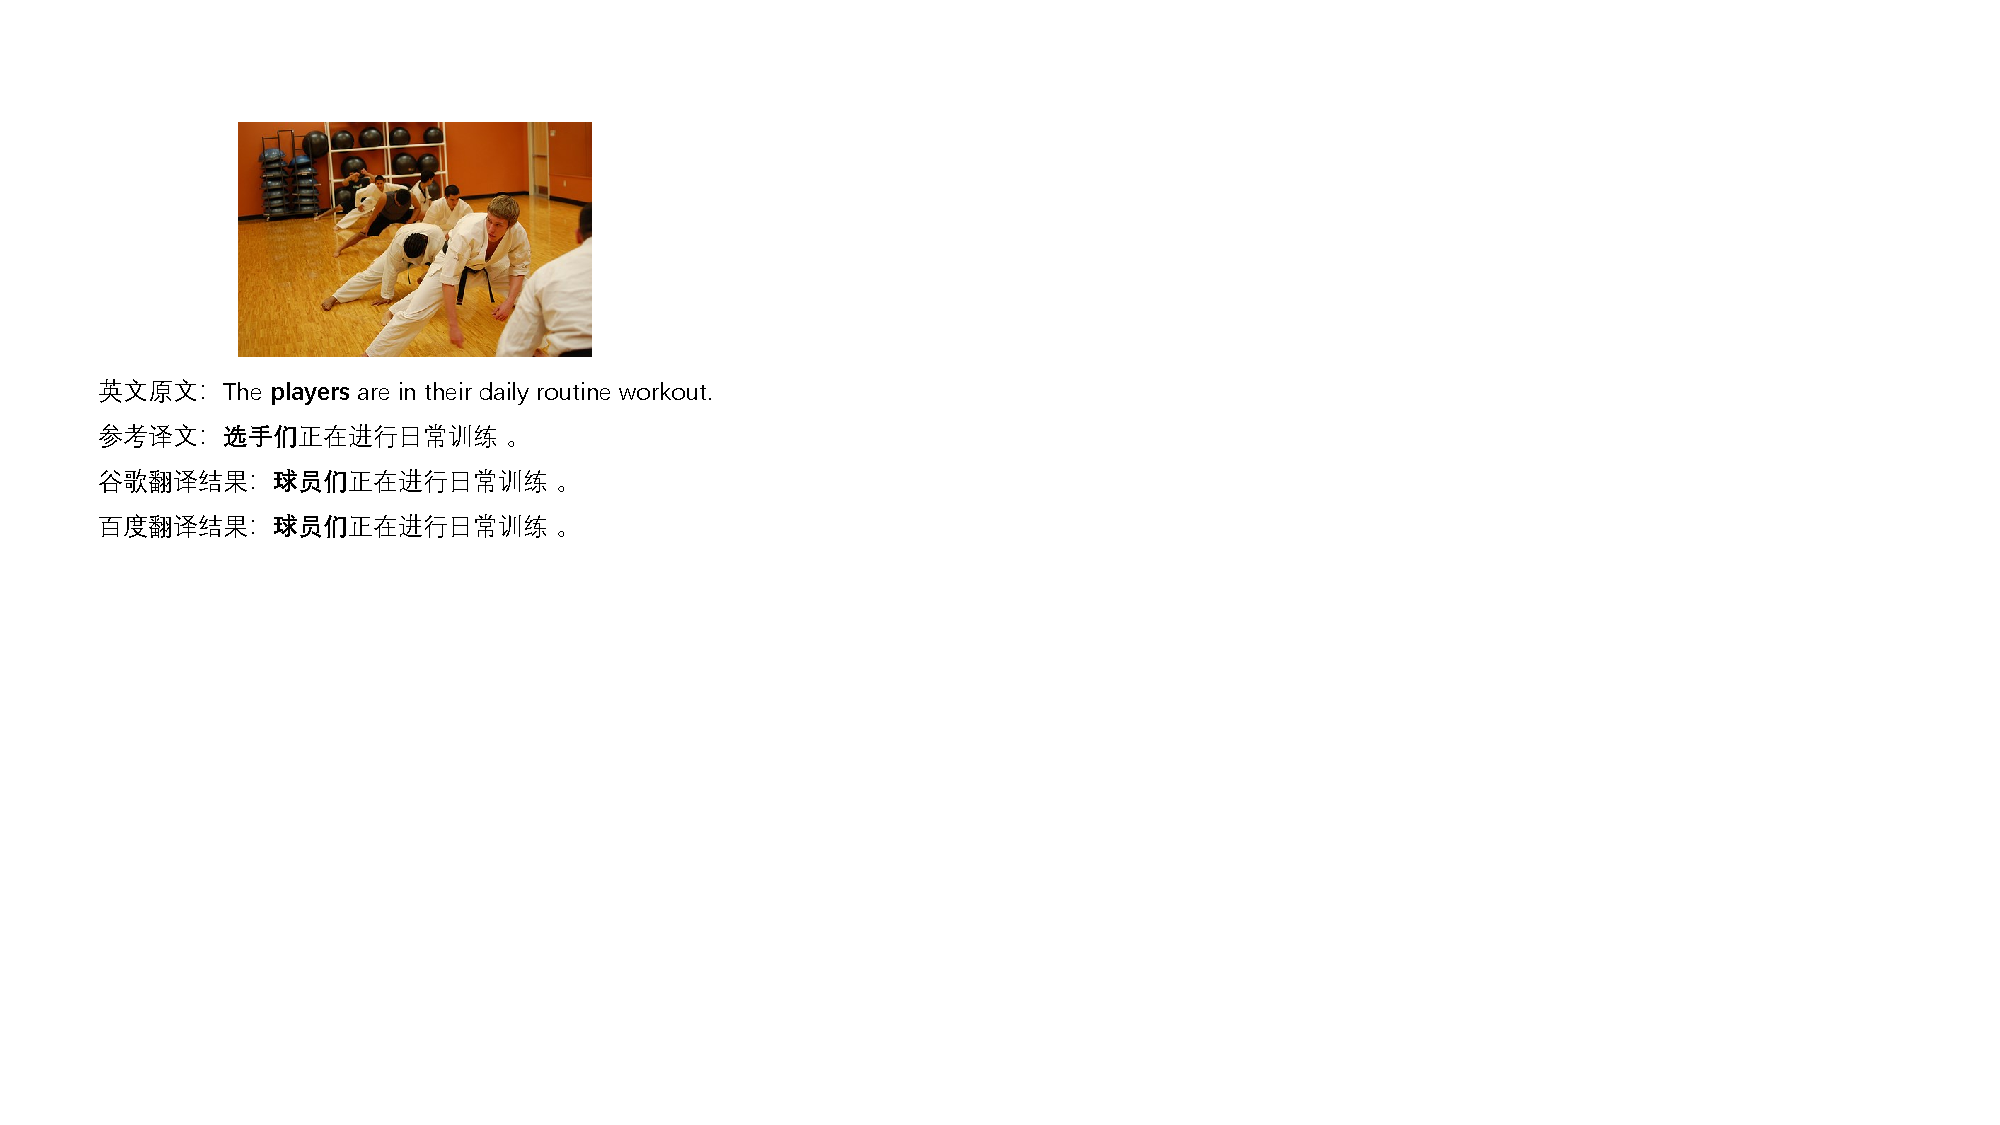
\includegraphics[width=0.75\linewidth]{Img/fig_1_case_players.pdf}
      \caption{错翻单词“players”}
      \label{fig:1_players}
    \end{subfigure}%
    \\
    \begin{subfigure}[b]{\linewidth}
      \centering
      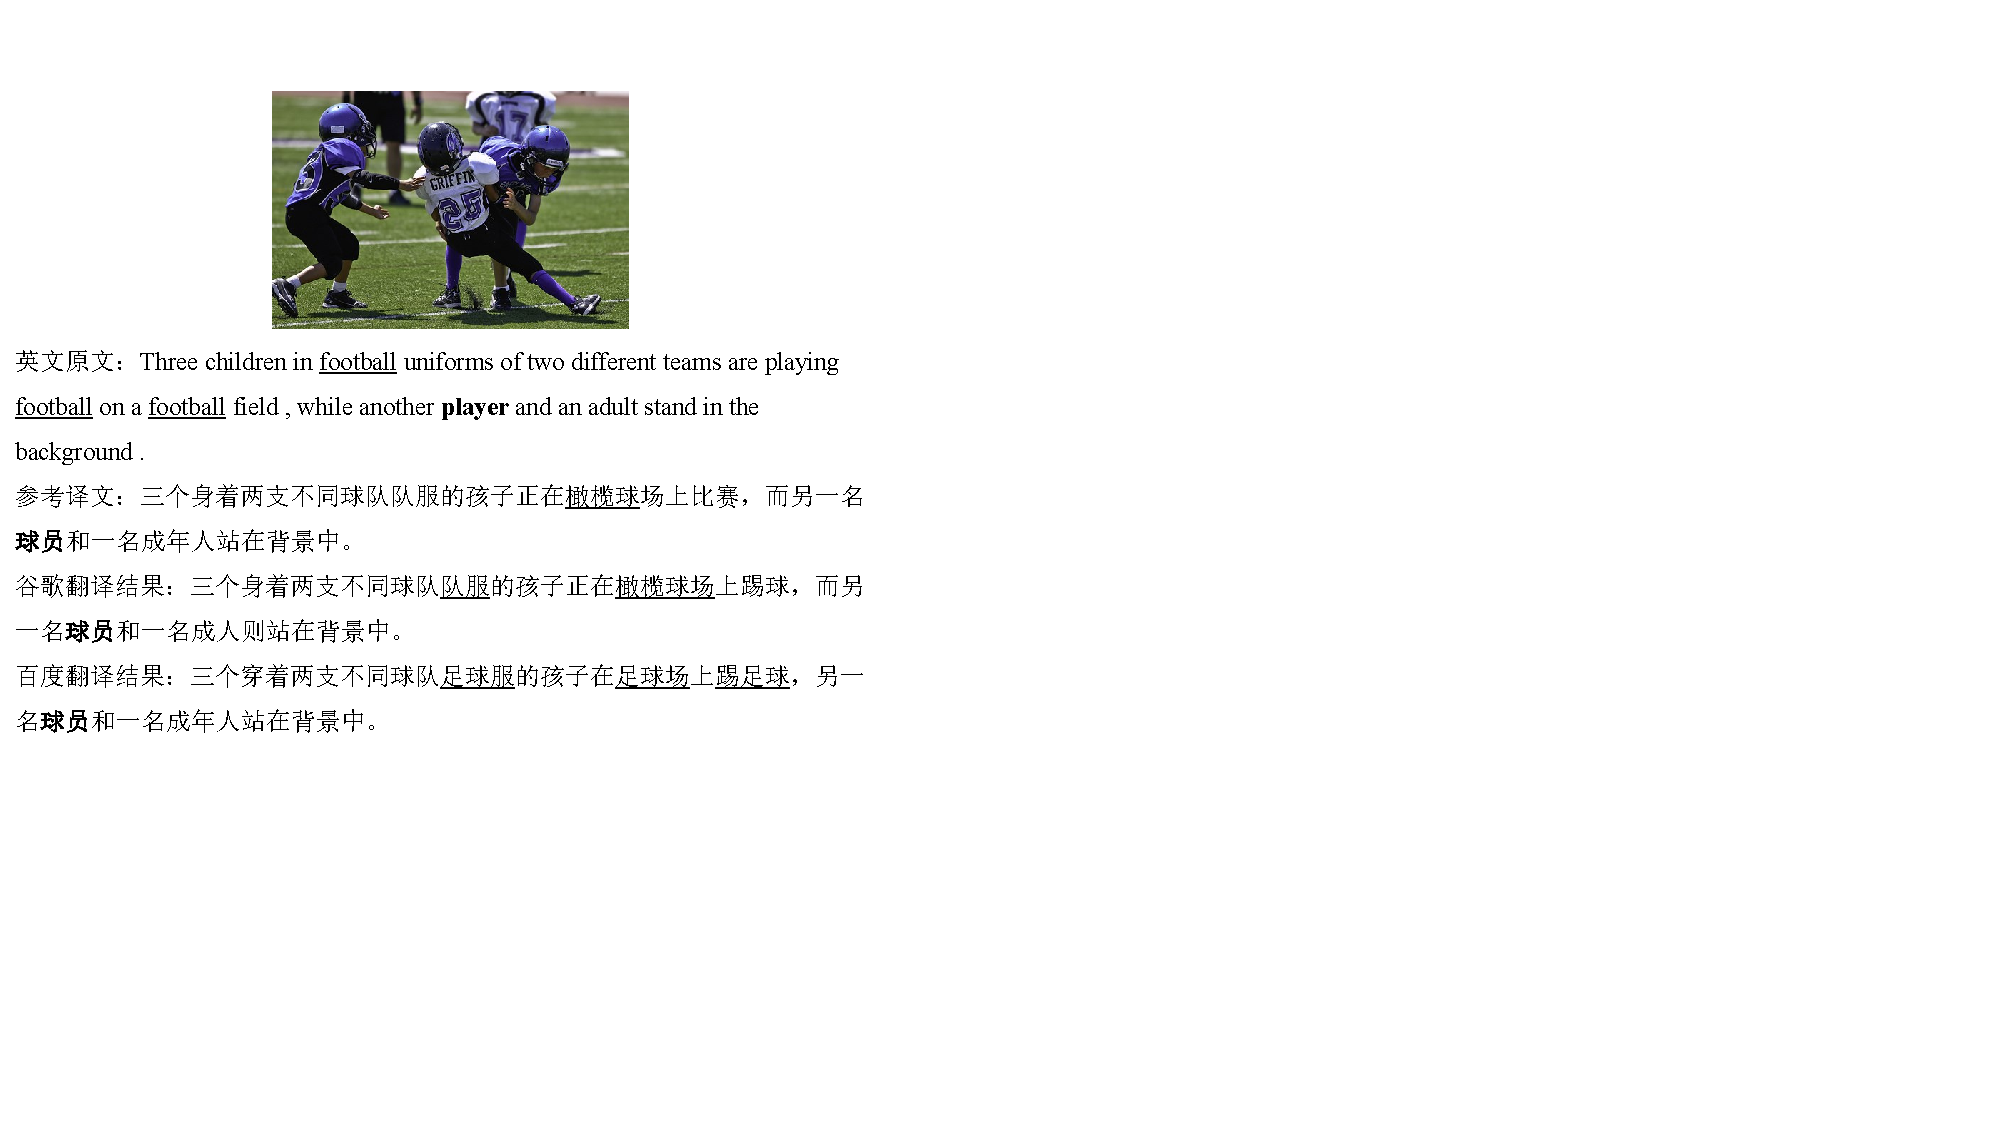
\includegraphics[width=\linewidth]{Img/fig_1_case_football.pdf}
      \caption{错翻单词“football”}
      \label{fig:1_football}
    \end{subfigure}
    \bicaption{翻译错误案例}{Cases of incorrect translation}
    \label{fig:1_translation_cases}
\end{figure}
图\ref{fig:1_translation_cases}给出了谷歌和百度的机器翻译系统对两句英文图片描述的翻译结果。
在图\ref{fig:1_players}中展示了一个简单却缺少上下文信息的翻译例子,加粗项“players”在实际应用中随着背景信息的变化可以有多种不同的释义,在图例中应指的是“空手道选手们”。然而,在不考虑图片所提供信息的情况下,两个纯文本机器翻译系统均将其翻译为更常见的释义“球员们”。仅从文本的角度考虑,该翻译结果并不差,但因为文本所提供的信息是不完整的导致其翻译结果与真实释义存在一定的差距。
图\ref{fig:1_football}的例子中同时包含了“football”(下划线项)和“player”(加粗项)两个容易翻译错误的地方。从谷歌和百度翻译系统的结果中可以看到,在不提供图片信息的情况下,谷歌翻译系统将“football”翻译为“橄榄球”,而百度翻译系统将其翻译为“足球”。在未提供图片信息的情况下,不同的翻译系统表现出了不同的倾向性,仅从文本信息的角度两者都是正确的翻译。在图\ref{fig:1_football}的例子中“player”翻译到了正确的“球员”释义。其原因可以归结为两点,一是如同图\ref{fig:1_players}的例子一样,翻译系统选择了更为常用的“球员”释义;二是翻译系统捕捉到了整段原文中提供的有关于“球”的上下文信息,从而得到了正确的翻译。

上述例子表明,当句子中存在多义词、歧义词、语义不完整等问题时,图片中所包含的视觉信息能够作为翻译过程中所需要的上下文信息,而常规的神经机器翻译系统不具备建模和利用来自其它模态的信息的能力。在真实的应用场景中,翻译系统要处理的可能是商品介绍、聊天记录、网络简讯等有匹配图文的句子。因此,探索融合图片信息的神经机器翻译方法具有重要的理论研究和实际应用价值。图片中包含着更丰富、更完整以及更准确的信息能够为句子的翻译提供更适合的上下文语境,帮助模型得到优化的编码表示,或是为模型解码提供视觉信息作为参考。

相比于统计机器翻译,在神经机器翻译中融合来自图片中的信息是更方便且更自然的,这也推动了ImgNMT的研究热潮,相关研究大量涌现。目前的ImgNMT方法主要关注针对图片描述的翻译中,如何利用图片信息改进翻译质量。图片描述的翻译任务中,句子与图片具备语义上的一致性,图片与句子之间语义融合的研究可以从更多的角度展开,其相关研究成果与结论也可以更方便的应用到其它领域。相关的模型方法主要关注图片信息在神经机器翻译模型中的利用,提出了各具特点的网络结构以及采用各种图片输入方式来建模视觉上下文信息,从而方便图片信息在神经机器翻译模型中的利用。然而,神经网络方法为跨模态信息融合带来便利的同时,也极大地削弱了各种模型方法的可解释性。存在大量的方法对翻译质量的提升有限,但却因为图片信息作用方式不明确的原因,难以进行针对性的改进。另外,NMT所采用的平行翻译数据一般具有良好的语义对齐特性。相比之下,句子与图片之间的语义对齐关系则更为复杂。这使得一般的ImgNMT模型在训练阶段很容易收敛为一个忽略了图片信息的纯文本翻译模型,导致模型在应用测试阶段也仅是将输入的图片输入作为噪声。
因此,本文主要从模型层面出发,针对目前融合图片信息的神经机器翻译方法利用图片信息方式的缺陷,探索更有效的跨模态信息融合方法,从而提升神经机器翻译的译文质量。


\section{研究内容}

本文的研究旨在改善目前融合图片信息的神经机器翻译方法中图片信息的作用方式,提升图片与文本在语义融合过程中的作用程度,从而达到提升译文质量的目的。本文的研究内容主要包括:如何将图片信息明确地作用在句子中的对应目标;如何进一步改进明确的视觉信息作用方式,将其与常规的跨模态信息融合方法相结合;如何提升常规跨模态信息融合方法中图片信息的作用程度,利用更多的视觉信息改善翻译质量。

具体地,本文的主要工作可以划分为以下三个部分:


{\sffamily 1. 基于跨模态文本重构的神经机器翻译方法}

将图片输入到神经机器翻译模型中具有直接从数据中学习并融合跨模态信息的优点,但也难以明确图片信息的具体作用,因此这类方法可称为隐式跨模态信息融合法。为了探究显式跨模态信息融合法是否可行,本文提出一种基于跨模态文本重构的神经机器翻译方法。该方法在训练中将源语言句子中的名词或短语的位置明确地替换为图片中对应的视觉目标,并将该序列输入到重构模型中用于生成原来的或目标语言的句子。最后通过参数共享的方式将重构模型的参数与翻译模型共享,达到提升翻译质量的目的。实验表明,本文所提方法在测试阶段不需要输入图片的情况下达到与隐式方法可比的翻译准确率。并且该方法主要提升了与视觉目标相对应的实体词的翻译准确率。

{\sffamily 2. 基于双向跨模态实体重构的神经机器翻译方法}

显式跨模态信息融合法能够准确地将图片信息作用到目标词上,但是采用文本重构一方面仅应用了图像到文本单方向重构,另一方面视觉信息仅作用到了实体词上。为了在显式方法中更充分地利用图片信息,并融合隐式方法的优点,本文提出一种基于双向跨模态实体重构的神经机器翻译方法。该方法抛弃了文本级别的重构,在文本实体和视觉实体之间做双向重构。并增加了非实体的重构,使图片信息与文本上下文做进一步的信息融合。然后,将以上三种重构任务与翻译任务通过多任务学习的方式结合。实验表明,该方法在测试阶段不需要输入图片的情况下进一步地提升了机器翻译的质量。实验分析表明,双向实体重构与非实体重构的多任务组合方式使模型受益最大。

{\sffamily 3. 基于图文对比对抗训练的神经机器翻译方法}

虽然显式跨模态信息融合方法能够为神经机器翻译模型带来翻译质量的提升。但此类方法存在图片信息利用不充分的问题,而隐式方法普遍存在视觉信息在模型中难以起作用的问题。为此,本文提出一种基于图文对比对抗训练的神经机器翻译方法。为了拉近双语的语义关系,在编码端增加了图文与目标语言句子之间对比学习。并在负样本集中引入了包含源语言句子+错误图片对抗样本。为了将正负样本区分开,模型需要判断图片信息是否与源语言句子的语义一致。该方法会将图片信息融合到文本的表示中,从而提升视觉信息在模型中的作用程度。实验表明,在提升了翻译准确率的同时,所提方法在输入错误图片或不输入图片的情况下翻译质量明显下降。


\section{论文的组织结构}

围绕上述研究内容,本文共分为六章,具体的组织方式如下:

第1章为绪论部分。本章首先机器翻译以及融合图片信息的神经机器翻译的研究背景和意义进行介绍,并指出神经机器翻译方法在融合图片信息的过程中存在哪些问题,随后介绍了本文针对目前存在问题所做的研究内容,最后在本节介绍了论文的组织结构。

第2章为融合图片信息的神经机器翻译方法国内外研究现状。本章首先详细介绍了神经机器翻译模型的发展历程和基础的模型框架。然后介绍了在将图片信息传递给神经机器翻译模型前,有哪些计算机视觉基础模型可以为跨模态信息的融合提供便利。紧接着,对融合图片信息的神经机器翻译方法进行了分类介绍,包括图片信息辅助式方法、图片信息增强式方法、基于图片搜索的方法以及无监督方法。最后,分析了现有方法所面临的问题与挑战,进而引出本文所要开展的工作。

第3章介绍了基于跨模态文本重构的神经机器翻译方法。为了将图片信息明确地作用到文本中的对应目标上,本章首先介绍了图片中的视觉目标与文本中的词或短语的对齐方法,设计了图片目标在文本编码过程中的明确作用方式。然后设计了两种文本重构方案和三种参数共享方案将重构任务融合到文本翻译任务中。最后介绍了所提方法在英德翻译数据上的实验结果。

第4章介绍了基于双向跨模态实体重构的神经机器翻译方法。为了进一步挖掘采用明确方式融合图片信息方法的潜能,本章首先介绍了文本实体到图片实体和图片实体到文本实体两个方向的实体级重构方案。为了充分利用图片中的视觉信息,将视觉信息与文本上下文融合,本章还介绍了非实体的重构方案。然后将以上三种重构方法以多任务学习的方式与翻译任务相结合。最后介绍了此多任务方法在三个翻译对上的有效性。

第5章介绍了基于图文对比对抗训练的神经机器翻译方法。为了在图片与文本信息融合过程中,使模型对图片中所包含的信息更敏感,本章首先介绍了一种在对比学习中加入对抗样本作为负样本的方法。然后在多个语言对上测试了所提方法提升翻译准确率的能力。最后分析了,对比对抗训练方法能否提升图片在神经机器翻译中的作用。

第6章对本文的研究工作进行总结,分析现有研究工作的不足,并对未来的研究工作进行展望。
\chapter{研究现状综述}\label{chap:relatedwork}

% 2.1 引言
\section{引言}
% 任务背景
% 可以介绍统计机器翻译到神经机器翻译的变革,带来了哪些影响,例如在多模态融合等方面的影响
机器翻译是一种利用计算机算法将一种语言翻译到另一种语言的技术。从统计机器翻译时代,到神经机器翻译时代,机器翻译相关技术一直作为行业的风向标引领着整个自然语言处理领域的发展。其基础模型从做到打破语言壁垒突破至跨越模态整合,能够在计算机视觉、语音信号处理以及多模态信息融合等领域都得到广泛的应用。
% 任务起源
% 可以提到机器翻译的缺陷,比如歧义、信息不充足等问题试图通过外源信息来解决
多模态机器翻译(Multi-modal Machine Translation,MMT)就是一种在机器翻译的基础上,融合图像信息、语音信息或者文档上下文信息的一类方法。这些引入的外源信息,在理论上具有解决歧义、转录错误以及指代不明等问题的意义。

% 任务形式
% 讲讲与机器翻译的区别、如何将其分为了两大类。
融合图片信息的神经机器翻译是一种将图片作为外源辅助信息输入到神经机器翻译模型中,以实现提升翻译准确率的一类方法。因此,与一般的机器翻译相似的是,相关研究所使用的语料同样需要平行翻译句对的形式,区别在于增加了与文本内容高度相关的图片输入。根据图片信息的作用方式,可以将相关方法分为图片信息辅助式、图片信息增强式和图片搜索式三类。本章将简要介绍神经机器翻译的发展过程,然后按照图片信息辅助式、图片信息增强式和图片搜索式的分类,分别介绍融合图片信息的机器翻译随着神经机器翻译的发展而进行改进与进化。

% 2.2 神经机器翻译
\section{神经机器翻译模型}
在融合图片信息的机器翻译任务中,平行翻译句对的原文与译文之间一般具有很强的对齐关系,而图片主要起到补充信息的作用。因此,该任务所使用的模型多数是以NMT的模型作为基础框架,视觉特征作为模型的额外输入。本节将介绍MMT在模型设计发展过程中所应用到的NMT基础模型框架,这其中包含:基于循环神经网络(Recurrent Neural Network,RNN)方法的NMT模型、增加注意力机制的基于RNN的NMT模型以及基于自注意力机制的Transformer。另外,还有基于卷积神经网络(Convolutional Neural Networks,CNN)的NMT模型\cite{6_DBLP:journals/corr/GehringAGYD17},但其很快被自注意力机制取代,也没有在MMT任务上的应用,因此本节忽略这部分内容的介绍。

\subsection{循环神经网络}
神经机器翻译是一种序列到序列的生成任务,其源端序列与目标端序列的长度往往是不同的。因此,编码器-解码器结构成为了神经机器翻译的常用模型框架。编码器和解码器分别用于编码源端序列和解码到目标端序列。循环神经网络就是一种用于解决序列建模的一类方法。图1为基于循环神经网络的神经机器翻译(RNN-based NMT,RNMT)框架。编码器将不定长的源语言句子编码为单个固定维度的隐层向量,该隐层向量可作为整个句子语义的特征表示。解码器负责根据该特征表示生成目标语言句子。形式化地,给定待翻译的源语言句子$X=\{x_1,x_2,…,x_n\}$,在编码端首先需要将$X$中的词转化为词向量$E=\{\boldsymbol{e}_1,\boldsymbol{e}_2,…,\boldsymbol{e}_n\}$,其中:
\begin{equation}
    \boldsymbol{e}_i=\mathrm{Emb}(x_i)
\end{equation}

源语言句子中的每个词$x_i$均有一个对应的词向量表示$\boldsymbol{e}_i$。然后编码器按照句子中词的顺序将句子编码到一个隐层状态序列$\overrightarrow{\boldsymbol{H}}={\overrightarrow{\boldsymbol{h}}_1,\overrightarrow{\boldsymbol{h}}_2,…,\overrightarrow{\boldsymbol{h}}_n}$,其中,$\overrightarrow{\boldsymbol{h}}_i$中编码了输入序列中前$i$项的信息,即:
\begin{equation}
    \overrightarrow{\boldsymbol{h}}_i=\mathrm{RNN}(\overrightarrow{\boldsymbol{h}}_{i-1},\boldsymbol{e}_i)
\end{equation}
为了使每个位置的编码结果融合到整个输入序列的信息,可采用双向编码器将句子$X$同时编码到$\overrightarrow{\boldsymbol{H}}$和$\overleftarrow{\boldsymbol{H}}$,其中,$\overleftarrow{\boldsymbol{H}}=\{\overleftarrow{\boldsymbol{h}}_1,\overleftarrow{\boldsymbol{h}}_2,…,\overleftarrow{\boldsymbol{h}}_n\}$为$X$的逆序编码结果,即:
\begin{equation}
    \overleftarrow{\boldsymbol{h}}_i=\mathrm{RNN}(\overleftarrow{\boldsymbol{h}}_{i+1},\boldsymbol{e}_i)
\end{equation}
将$\overrightarrow{\boldsymbol{H}}$和$\overleftarrow{\boldsymbol{H}}$拼接得到$\boldsymbol{H}=\{\boldsymbol{h}_1,\boldsymbol{h}_2,\cdots,\boldsymbol{h}_n\}$, 其中:
\begin{equation}
    \boldsymbol{h}_i=[\overrightarrow{\boldsymbol{h}}_i;\overleftarrow{\boldsymbol{h}}_i]
\end{equation}

RNMT的解码器同样采用循环神经网络来生成目标语言文本。该生成翻译的过程是自回归的,即在时刻$t$,解码器需要根据$0$至$t-1$时刻的解码结果及源语言所提供的上下文信息来生成当前时刻的预测结果:
\begin{equation}
    \boldsymbol{s}_t=\mathrm{RNN}(\boldsymbol{s}_{t-1},y_{t-1})
\end{equation}
\begin{equation}
    P(y_t|y_{<t},X)=\mathrm{softmax}(g(\boldsymbol{s}_t, y_{t-1}, \boldsymbol{c}_t))
\end{equation}
该过程中,源端上下文信息的作用方式有很多种。文献\cite{1_DBLP:journals/corr/SutskeverVL14}将$\overrightarrow{\boldsymbol{h}}_n$传递给解码器作为初始状态$\boldsymbol{s}_0$。文献\cite{2_cho-etal-2014-learning}将$0$至$t-1$时刻的解码结果编码,并连同源端上下文信息$\boldsymbol{H}$预测当前时刻单词:
\begin{equation}
    \boldsymbol{c}_t=f(\boldsymbol{H})
\end{equation}
其中,$f(\cdot)$表示选用平均池化(average pooling)对$\boldsymbol{H}$取平均,或直接选取$\boldsymbol{H}$的最后一项$\boldsymbol{h}_n$。

尽管基于循环神经网络的神经机器翻译还没有实现对传统统计机器翻译在翻译准确率上的全面超越,但其采用的编码器-解码器框架已经展现了能够将文本数据进行分布式表示并从这种表示中解码到目标语言译文的能力。这种分布式表示方法也为跨模态信息的融合提供了极大的便利。

\subsection{注意力机制}
基于编码器-解码器结构的神经翻译模型利用编码器将源语言编码为一个固定的特征向量,再利用解码器中的循环神经网络编码已生成的目标端词元,从而指导新的目标端词元的生成。在该过程中,编码的源语言特征向量作为句子级语义的完整表示,一方面丢失了源语言中的句长信息,另一方面无法指导在当前时刻$t$生成目标端词元时,应该更多地关注源端的哪些信息。为了解决该问题,文献\cite{3_DBLP:journals/corr/BahdanauCB14}提出在编码器与解码器之间增加注意力机制(attention mechanism)。

图2为增加了注意力机制的神经机器翻译,其编码器和解码器保留原来的工作方式,而两者之间的注意力模块为解码器提供了动态的源语言上下文信息。对于每个时刻$t$,源语言上下文向量$\boldsymbol{c}_t$由固定的特征向量替换为与$t$相关的表示:
\begin{equation}
    \boldsymbol{c}_t = f_t(\boldsymbol{H})=\sum_{i=1}^{n}{\alpha}_{ti}\boldsymbol{h}_i
\end{equation}
\begin{equation}
    {\alpha}_{ti}=\frac{\mathrm{exp}(a_{ti})}{\sum_{j=1}^{n}\mathrm{exp}(a_{tj}}
\end{equation}
文献\cite{3_DBLP:journals/corr/BahdanauCB14}中:
\begin{equation}
    a_{ti} = \mathrm{score}(\boldsymbol{s}_{t-1},\boldsymbol{h}_i)
\end{equation}
其中$\mathrm{score}(\cdot)$是打分函数,计算两个向量所携带信息的相关程度,可采用点积或多层感知机等方法。上式对$\boldsymbol{s}_{t-1}$和$\boldsymbol{h}_i$进行打分,表示根据已生成的目标文本的编码表示$\boldsymbol{s}_{t-1}$,来计算源语言中第$i$项对当前时刻$t$的重要程度。因此,$a_{ti}$代表着生成$t$时刻的目标端词元时,对源语言中第$i$项的“关注”度,${\alpha}_{ti}$就是该“关注”度的归一化的结果,$\boldsymbol{c}_t$就是根据“关注”度对特征向量的加权表示。

值得注意的是,$t-1$时刻的输出结果$y_{t-1}$是由$\boldsymbol{s}_{t-1}$得到的,因此上式中丢失了$y_{t-1}$的信息,因此文献\cite{4_luong-etal-2015-effective}提出了改进方案:
\begin{equation}
    a_{ti} = \mathrm{score}(\boldsymbol{s}_{t},\boldsymbol{h}_i)
\end{equation}
并规定了$\mathrm{score}(\cdot)$的三种计算方式,综合文献\cite{3_DBLP:journals/corr/BahdanauCB14},可得到以下四种方法:
\begin{equation}
    \mathrm{score}(\boldsymbol{s}_t, \boldsymbol{h}_i) = 
    \begin{cases}
        \boldsymbol{s}_t^T \boldsymbol{h}_i & \mbox{点积法} \\
        \boldsymbol{s}_t^T \boldsymbol{W}_a \boldsymbol{h}_i & \mbox{通用点积法} \\
        \boldsymbol{W}_a[\boldsymbol{s}_t; \boldsymbol{h}_i] & \mbox{连接法} \\
        \boldsymbol{v}_a^T \mathrm{tanh}(\boldsymbol{W}_a \boldsymbol{s}_t+\boldsymbol{U}_a \boldsymbol{h}_i) & \mbox{多层感知机法} 
    \end{cases}
\end{equation}
其中$\boldsymbol{v}_a$、$\boldsymbol{W}_a$和$\boldsymbol{U}_a$是网络参数,$T$表示对向量进行转置。

%(注意力机制在视觉领域的应用,以及在跨模态领域的应用。)

\subsection{Transformer}
在注意力机制的帮助下,基于循环神经网络的机器翻译得到了显著的性能提升。这说明基于动态上下文的解码方法能够更准确地捕捉上下文信息,从而得到更忠于原文的译文。而注意力机制相当于二次编码,为下游模块提供动态上下文。既然注意力机制同样具有编码能力,那么是否可以用于替换循环神经网络呢?谷歌提出的Transformer\cite{5_DBLP:journals/corr/VaswaniSPUJGKP17}就是一种基于这种假设的模型。图3展示了Transformer的模型结构,其保留了编码器-解码器的基础框架,利用内置的多头注意力机制(multi-head attention mechanism)实现编码过程。

区别于一般的注意力机制,多头注意力机制采用了一种更具泛化性的模型设计。如图4所示,多头注意力机制的输入分为查询(Query,$\boldsymbol{Q}$)、键(Key,$\boldsymbol{K}$)以及值(Value,$\boldsymbol{V}$)三部分,并结合了缩放点积注意力(scaled dot-product attention)和多头注意力(multi-head attention)两种方法。

缩放点积注意力:与一般的点积法相比,缩放点积注意力增加了一个缩放因子$d_k^{-0.5}$:
\begin{equation}
    \mathrm{Attention}(\boldsymbol{Q},\boldsymbol{K},\boldsymbol{V}) = \mathrm{softmax} \left( \frac{\boldsymbol{Q}\boldsymbol{K}^T}{\sqrt{d_k}} \right) \boldsymbol{V}
\end{equation}
其中,$d_k$代表$\boldsymbol{Q}$、$\boldsymbol{K}$和$\boldsymbol{V}$的隐层维度。采用点积法的优点在于点积是以矩阵乘的形式进行计算,通过代码优化等方法可以很好地对矩阵乘进行硬件加速。引入缩放因子则是为了防止$d_k$较大时,点积的数值膨胀导致$\mathrm{softmax}(\cdot)$函数逼近梯度消失的数值范围。

多头注意力:为了丰富动态上下文所承载的信息,文献\cite{5_DBLP:journals/corr/VaswaniSPUJGKP17}将多个注意力模块拼接组成多头注意力机制:
\begin{equation}
    \mathrm{MultiHead}(\boldsymbol{Q},\boldsymbol{K},\boldsymbol{V}) = \mathrm{Concat}(\boldsymbol{head}_1, \cdots, \boldsymbol{head}_n)\boldsymbol{W}^O
\end{equation}
\begin{equation}
    \boldsymbol{head}_i = \mathrm{Attention}(\boldsymbol{Q}\boldsymbol{W}_i^Q,\boldsymbol{K}\boldsymbol{W}_i^K,\boldsymbol{V}\boldsymbol{W}_i^V)
\end{equation}
其中,$\boldsymbol{W}_O$,$\boldsymbol{W}_i^Q$,$\boldsymbol{W}_i^K$和$\boldsymbol{W}_i^V$是模型参数。$\boldsymbol{Q}$、$\boldsymbol{K}$和$\boldsymbol{V}$经过不同的参数映射到不同的表示空间,再由注意力机制编码得到的不同的上下文特征表示。该过程相当于在不增加额外参数的情况下,将多个模型集成到一个模型中,从而提升模型的学习能力。

多头注意力机制在Transformer中的用途分为三种:
\begin{itemize}
    \item 位于编码器的多头自注意力机制用于编码源语言句子,此时Transformer编码器第一层的$\boldsymbol{Q}$、$\boldsymbol{K}$和$\boldsymbol{V}$均为源语言句子经映射后的词向量序列,其它层的$\boldsymbol{Q}$、$\boldsymbol{K}$和$\boldsymbol{V}$为前一层的输出。
    \item 位于解码器中带有掩码的多头自注意力机制用于编码目标端已经解码出来的部分句子。掩码的作用是为了保持自回归解码过程中后面位置词元的解码只能用到前面位置的信息的特性。
    \item 连接编码器与解码器的多头交叉注意力机制的作用和一般的注意力机制一致。此时$\boldsymbol{Q}$为解码器中带有掩码的多头自注意力机制的输出,$\boldsymbol{K}$和$\boldsymbol{V}$为编码器的隐层输出。交叉注意力机制输出的是融合了源端信息的目标端句子的表示。
\end{itemize}
值得注意的是,基于注意力机制的编码与循环神经网络相比丢失了对输入序列位置信息的建模。因此,文献\cite{5_DBLP:journals/corr/VaswaniSPUJGKP17}提出了位置编码,为每个词向量增加位置信息。%文献\cite{DBLP:journals/corr/GehringAGYD17}则提出了更为方便的位置词向量的方案。

尽管近年来针对Transformer框架的改动层出不穷,但广泛应用的模型基本保持了最原始的设计方案。常见的改动如文献\cite{7_DBLP:conf/naacl/DevlinCLT19}提出了使用位置词向量的方式替换位置编码,文献\cite{8_DBLP:journals/corr/abs-1803-02155,9_DBLP:journals/corr/abs-1901-02860}为了加强Transformer长序列编码能力提出了相对位置编码。而这些创新性的改动基本都保留了Transformer中的自注意力机制和交叉注意力机制的基本结构。在大规模预训练任务的表现上,Transformer更是充分展现了其应用场景的灵活性。针对不同规模的数据,通过增减参数规模的方式就可以使其适应相应的任务。相比于基于循环神经网络的模型,Transformer能够容纳更长的输入序列和更大规模的网络参数。

Transformer出色的编码能力不仅在自然语言处理任务大放异彩,还在计算机视觉以及多模态信息融合等领域展现了不俗的潜能。文献\cite{10_DBLP:journals/corr/abs-1802-05751,11_DBLP:conf/iclr/DosovitskiyB0WZ21,12_DBLP:conf/iccv/LiuL00W0LG21,13_DBLP:conf/iccv/0007CWYSJTFY21}摒弃了传统基于卷积神经网络的方法,直接采用Transformer作为图像分类、目标检测以及语义分割等计算机视觉任务的基础模型,并得到了进一步的性能提升。文献\cite{14_DBLP:conf/nips/LuBPL19,15_DBLP:conf/eccv/ChenLYK0G0020,16_DBLP:journals/corr/abs-2004-00849,17_DBLP:conf/icml/KimSK21}则是在大规模文本预训练模型的基础上,在输入序列中增加图片输入或从图片中提取的视觉目标,来提升Transformer在多模态自然语言理解(multi-modal natural language understanding)任务上的能力。

%(Transformer已经在业界产生的影响力,自注意力替换循环神经网络的必要性,解决了哪些问题)

% 2.3 visual guided MMT
\section{图片信息辅助式神经机器翻译}
得益于神经网络方法的快速发展,自然语言文本与图片的信息融合成为了可能。融入图片信息的机器翻译的研究历程也紧随着纯文本的神经机器翻译的脚步而发展。然而,相关研究则最早起源于图像描述生成任务。有部分学者将文本作为一个外源信息来辅助图片描述的生成,但这种方式的本质则是在翻译任务中融入视觉信息。2016年WMT将多模态机器翻译引入作为共享任务后,MMT受到了广泛的关注。在之后的WMT17和WMT18,MMT任务延续并奠定了在机器翻译中融合图片信息作为多模态机器翻译研究的主要范式。

%平行翻译句一般具有良好的对齐特性,这使得融入的外源信息仅用于辅助少数具有歧义、信息不完整以及训练不充分等问题的句子的翻译。该特性也成为了展开相关研究道路上的一大难点。
融合图片信息的神经机器翻译任务主要采用的是平行翻译句对加图片三元组形式的数据,即一张图片对应一句描述和一句翻译。大部分相关研究需要对神经机器翻译模型进行适当的修改,以适应图片的输入。模型中输入的图片可用于辅助优化翻译过程中源语言的语义表示,或为解码过程增加辅助外源信息。本文将这种在翻译过程中以源端文本作为信息主体,输入图片用于语义信息强化的方法称为图片信息辅助式神经机器翻译。可根据图片信息融合到翻译模型中的方式将这种方法分为三类:融合图片全局信息、融合图片局部动态信息以及融合图片视觉目标信息。这些三种图片信息以视觉特征为载体输入到翻译模型中,视觉特征则是从预训练的卷积神经网络中提取得到。不同的提取方式所包含的语义信息的粒度和特征维度有所不同。将这些不同形式的视觉特征整合到NMT模型后,模型进行跨模态语义融合的难易程度则取决于模型设计的合理性。

\subsection{融合图片全局信息的神经机器翻译}

\cite{18_DBLP:conf/emnlp/CalixtoL17}
\cite{19_DBLP:conf/acl/CalixtoRA19}
\cite{20_DBLP:conf/acl/WuKBLK20}


\subsection{融合图片局部动态信息的神经机器翻译}

\subsection{融合图片视觉目标信息的神经机器翻译}



% 2.4 visual enhanced MMT
\section{图片信息增强式神经机器翻译}
% 2.5 retrieval-based MMT
\section{基于图片搜索的神经机器翻译}





\section{本文研究思路}

% MMT的演变与拥有的优势
% MMT现有存在的问题
从基于循环神经网络的RNMT,到目前广泛采用的Transformer,研究者们致力于将图片中的视觉信息以各种方式融合到翻译过程中,从而提升机器翻译的质量。这是因为,相比于纯文本,图片中往往包含更完整、更细节以及更丰富的语义信息。然而,相比于纯文本翻译利用端到端模型就可以学习到跨语言的表示与生成,融入图片信息的神经机器翻译并不是简单地将图片输入到模型中就能够将跨模态的信息进行融合并利用。

得益于不同模态的信息在神经网络方法中普遍以分布式向量表示的形式呈现,在神经翻译模型中实现跨模态信息融合具有很强的优势:1)能够直接从数据中学习数据特征,不需要人为的特征设计;2)采用成熟的神经翻译模型作为主框架,采用预训练的卷积神经网络用于图片编码,跨模态信息融合可以在现有模型基础上进行改进;3)图片作为上下文信息的表示方法与融合方式,和一般的文档上下文或视频上下文类似,相应的模型方法有很强的泛化复用性;4)解决歧义词或语义不完整等文本中出现信息缺失的问题。

% 本文索要解决的问题:三篇文章
然而,已有方法同样存在一些问题,例如翻译质量的提升不稳定,图片信息的作用方式不明确,翻译模型对视觉信息不敏感等问题。尽管当前广泛应用的神经翻译模型与计算机视觉基础模型为跨模态信息融合提供了极大的便利,依旧难以针对不同跨模态信息需求的文本翻译数据设计统一的模型方案。为此,本文尝试回答三个问题:
\begin{itemize}
    % 输入图片不一定带来提升
    \item {\sffamily 翻译质量提升不稳定}。文献\cite{21_dutta-chowdhury-elliott-2019-understanding,22_li-etal-2021-vision,20_wu-etal-2021-good}的实验表明,相比于纯文本神经翻译,输入图片信息后的翻译模型的翻译准确率并没有得到明显的提升,有些甚至会低于纯文本翻译。这说明在一般的翻译模型中,将图片中的视觉信息与文本信息的融合并不是一个必然的过程。如何使融合图片信息的神经机器翻译获得有效的翻译准确率的提升?
    % 隐含式方法的弊端
    \item {\sffamily 图片信息作用方式不明确}。尽管已有很多模型方法表明输入图片信息能够为翻译质量带来提升,然而图片信息的作用方式并不明确。例如,歧义词问题是否得到解决?语义不完整的句子是否得到补全?亦或是在其它不得而知的方面为翻译带来的增益?如何以更明确的方式将视觉信息作用到神经翻译中?
    % 输入噪音可能比输入图片带来的提升更多
    \item {\sffamily 翻译模型对视觉信息不敏感}。文献\cite{23_elliott-2018-adversarial}将与文本内容不一致的图片输入到翻译模型中来测试模型翻译准确率的提升是否来自于图片中的视觉信息,实验结果显示大部分模型可以从错误的图像中获得同样或相近的翻译准确率的提升。文献\cite{20_wu-etal-2021-good}认为输入图片与输入早已的作用相似,是正则化作用而非视觉信息为模型带来的翻译准确率的提升。如何使翻译模型对输入图片信息敏感?
\end{itemize}

为此,本文围绕融合图片信息的神经机器翻译方法研究,从改进模型的训练方式、图片的输入方式、视觉信息的作用方式等方面展开研究工作:
\begin{itemize}
    % 翻译质量提升不稳定,作用方式不明确
    \item {\sffamily 基于跨模态文本重构的神经机器翻译:}为解决图片信息作用方式不明确的问题,改变了图片的输入方式,使用图片的视觉目标特征以替换的方式作用到名词短语或名词两种粒度上,用于重构完整的文本。然后改变了模型的训练方式,以多任务训练的方式,利用多模态重构任务优化神经机器翻译模型的表示能力,从而提升翻译的准确率,得到具有稳定提升翻译质量能力的神经翻译模型。第3章将介绍我们提出的基于跨模态文本重构的神经机器翻译方法。
    % 翻译质量提升不稳定,作用方式不明确
    \item {\sffamily 基于双向跨模态实体重构的神经机器翻译:}在上一部分工作的基础上,以更明确的方式,针对实体词和视觉实体,实现双向跨模态实体重构。区别于重构完整的文本,针对实体词即可得到较好的模型结果。第4章介绍我们提出的基于双向跨模态实体重构的神经机器翻译方法。
    % 翻译质量提升不稳定,对视觉信息不敏感
    \item {\sffamily 基于图文对比对抗训练的神经机器翻译:}在训练融合图片信息的神经翻译模型的同时,采用对比学习方法学习译文与多模态输入的联合语义表示空间。为了解决模型对视觉信息不敏感的问题,在对比学习的负样本集中加入图文不一致的对抗样本。通过提升翻译模型区分输入图片正确与否的能力,强迫模型将图片中的视觉信息融合到文本表示中,从而强化源端文本的特征表示,实现翻译准确率的提升。第5章将介绍我们提出的基于图文对比对抗训练的神经机器翻译方法。
\end{itemize}
%(在这里提到模型对视觉信息不敏感的问题,然后循序渐进讲为什么我们的研究以增强式为主,后又如何补充辅助式)

\section{本章小结}
本章介绍了与融合图片信息的神经机器翻译相关的国内外研究,其中包括神经机器翻译主流模型的发展过程。然后主要介绍了在神经翻译模型中融合图片信息的主流方法,以及各类方法所具备的特点。本章分析了现有融合图片信息的神经机器翻译方法的缺陷,简要地说明了相应的解决办法,以及针对这些问题本文的一些应对思路。这些内容与本文的研究内容息息相关,在后面的章节中,本文将针对如何将图片中的视觉信息融合到神经翻译模型中给出相应的解决方案。


\chapter{基于跨模态文本重构的神经机器翻译}
% 本文应该侧重的是:
%    明确的视觉信息融合方式;
%    短语和词级别的视觉信息融合;
%    模型不需要对视觉信息敏感,因为视觉信息直接作用到目标上了

% 摘要
% 原文摘要:现有多模态机器翻译将视觉信息以全局特征的方式作为固定上下文输入,或者利用注意力机制对图像建立动态上下文作为文本内容的补充信息。然而这种隐含式的视觉信息融合方法对于分析图像如何起到作用以及为什么会产生作用带来了很大的挑战。针对此问题,提出了一种实体级的跨模态信息融合方法,显式地将文本中实体替换为对应图像中的视觉目标,并利用翻译模型来重建出完整的原文本,最后通过多任务的方式将以上重建任务与翻译任务相结合。实验表明,该方法在有效的提升了实体词的翻译质量,译文质量得到了显著的提升。
% 
%现有融入图片信息的神经机器翻译将视觉信息以全局特征的方式作为固定上下文输入,或者利用注意力机制对图像建立动态上下文作为文本内容的补充信息。然而这种隐含式的视觉信息融合方法对于分析图像如何起到作用以及为什么会产生作用带来了很大的挑战。针对此问题,提出了一种实体级的跨模态信息融合方法,显式地将文本中实体替换为对应图像中的视觉目标,并利用翻译模型来重建出完整的原文本,最后通过多任务的方式将以上重建任务与翻译任务相结合。实验表明,该方法在有效的提升了实体词的翻译质量,译文质量得到了显著的提升。

% 神经机器翻译中融合图片信息的问题:普遍范式中,句子与图片的信息融合是隐式的,即无法准确得知视觉信息作用到哪些词上或对句子的表示带来了哪些影响,因此,为了探索是否能够以明确的方式融合视觉信息,明确方式融入视觉信息是否对翻译有效,本章提出了一种在名词短语或名词的粒度上融合图片中的视觉目标信息,并进行跨模态文本重构的重构任务。再通过多任务训练的方式,将重构任务所优化的模型参数与翻译任务共享,从而达到提升翻译质量的目的。本章设置了进一步的分析实验,实验结果表明本章所提方法通过有效的提升实体词的翻译质量,从而提升了翻译准确率。

% 多模态的好处
采用分布式向量表示的神经翻译模型和计算机视觉基础模型极大地便利了以句子为基本语义单位的跨模态信息融合,
% 研究现状
例如,将图片以全局特征的方式作为固定上下文输入到神经翻译模型中,或者利用注意力机制对图像建立动态上下文作为文本内容的补充信息。
% 存在的问题
然而在这些方法中,句子与图片的信息融合是隐式的,即无法准确得知视觉信息作用到哪些词上或对句子的表示带来了哪些影响。
% 本章提出的方法
因此,为了探索是否能够以明确的方式融合视觉信息,以及明确方式融入视觉信息是否能够带来稳定的翻译质量提升,本章提出了在词级和短语级融合图片中的视觉目标信息,并进行跨模态文本重构的重构任务。通过多任务训练的方式,将文本重构任务所优化的模型参数与翻译任务共享,从而达到提升翻译质量的目的。
% 进一步的分析结果
%本章设置了进一步的分析实验,实验结果表明本章所提方法通过有效地提升实体词的翻译质量,从而提升了翻译准确率。
本章设置了进一步的分析实验,实验结果表明所提方法对实体词的翻译有更好的提升效果,从而提升了译文的质量。

\section{引言}
% 背景:
得益于神经网络方法的快速发展,自然语言处理和计算机视觉等领域均得到了飞速的进步,同时也为跨领域的信息融合带来了可能。在神经机器翻译中融合图片信息就是其中一种跨模态信息融合方法。跨模态的信息融合是为了解决一些在翻译中难以解决的问题,例如文本中存在歧义,表达不完整,文本表示欠拟合等问题。图片中往往包含着更丰富的语义信息。因此,如何将图片信息融合到翻译中成为了研究者们所关注的问题,相关方法也层出不穷。

% 相关研究:
目前已有的研究主要关注如何将整个图片中的信息融合到神经机器翻译模型的翻译过程中。由于图像分类任务所使用的卷积神经网络,如Resnet-50\cite{32_DBLP:conf/cvpr/HeZRS16},取得了非常好的效果,因此多数研究这尝试将预训练的卷积神经网络与神经翻译模型相结合。例如部分研究将图片经过卷积神经网络提取得到全局特征后,将其作为一个包含完整的上下文信息的特征向量以各种方式输入到翻译模型中,从而完善翻译模型在编码过程所获得的语义表征或为解码过程提供外源信息以供参考\cite{52_DBLP:journals/corr/ElliottFH15,18_DBLP:conf/emnlp/CalixtoL17,22_li-etal-2021-vision,20_wu-etal-2021-good}。
文献\cite{36_calixto-etal-2017-doubly,47_DBLP:conf/wmt/LibovickyHM18}尝试利用图片局部特征与注意力机制配合获图片的局部动态上下文,以达到在解码过程中融合与当前解码步骤最相关的视觉信息。此类方法中,图片作为一个句子级别的语义信息提供者作用到翻译过程中,试图使翻译模型最大化地利用图片中所包含的信息。
%因视觉信息与文本信息的融合与利用为通过模型学习的方式,而难以明确图片信息在翻译中的作用过程,本文称此类方法为隐式跨模态信息融合方法。

% 存在的问题:
然而,这些方法均以隐式的方式将图片信息与文本信息相结合,这些融合图片信息的神经机器翻译模型是如何应用视觉信息以及为何输入图片能够使得翻译性能提升都是不明确的,本文中,我们称此类方法为隐式跨模态信息融合方法。更重要的是,部分方法存在翻译质量提升不稳定的情况,不同的模型实现方案或不同的模型初始化条件下模型的翻译性能表现差异较大。尽管在句子级语义单位可以最大化地利用图片中所携带的视觉信息,但神经翻译模型似乎不能很顺利地将其利用。

% 本章提出方法
为此,本章提出了一种明确的图片信息融合方法。文献\cite{53_caglayan-etal-2019-probing}发现,当文本中部分内容或信息缺失,尤其是实体词缺失时,神经翻译模型对视觉信息最敏感。为了将图片中的视觉信息明确并有效地融合到模型中,本文以实体为语义单元融合图片信息,其中实体以短语实体或名词实体两种粒度呈现。区别于文献\cite{53_caglayan-etal-2019-probing}通过创造的文本内容缺失环境使隐式跨模态信息融合有效,本文采用显式跨模态信息融合方法,直接利用视觉特征替换实体作为模型输入,规避了神经翻译模型对视觉信息不敏感的问题。为了实现跨模态的信息融合,本文设计了一个重构模型来实现多模态输入到纯文本输出的任务。该模型以图片的视觉目标联合实体被替换的源语言文本为输入,以原文或译文为输出,通过端到端的学习将视觉目标中的视觉信息融合到实体的表示中。最后,本文利用了多任务学习方法,将跨模态文本重构任务与翻译任务相结合。通过多种参数共享机制,使翻译模型能够充分利用到重构任务重所学习到的视觉信息,从而提升翻译质量。

本章主要贡献如下:

(1)本章提出了一种基于跨模态文本重构的神经机器翻译方法(neural machine translation based on cross-modal text reconstruction, CTR-NMT), 并且将所提方法应用到了RNMT和Transformer两种框架。本章详细对比了多种参数共享方案,在推断(inference)时没有额外的图片输入的情况下,达到了与其它模型可比的翻译准确率。与纯文本基线模型相比,有着稳定的翻译质量的提升。

(2)本章提出了一种明确的融合图片信息的方法,即显式跨模态信息融合法。将图片中的视觉目标信息明确的作用到在文本中相对应的实体上,并在基于短语和基于词两种粒度的跨模态融合方案进行了实验对比,发现相比于短语实体,在词实体上融合图片信息效果更佳。

(3)本章对视觉目标的作用对象进行了分析,并发现本章所提的明确的图片信息作用方法,使名词实体的翻译准确率得到了更进一步的提升,从而提升了神经机器翻译模型的翻译质量。

\section{相关工作}

% 相关工作分类:
%     传统方法:句子级融合法,隐式法,(Feature-level Incongruence Reduction for Multimodal Translation,直接使用视觉特征不适合当前模型)
%     重构法:文本重构(Neural Machine Translation with Reconstruction,
%            图像重构(mywork2)(Imagination,Adversarial reconstruction for Multi-modal Machine Translation
%     实体替换法:主要用于分析
%     视觉目标法:
%     预训练模型法:

% 这里可能需要提一下“退化文本”的概念
\section{实体对齐方法}
\label{sec:entity_extraction}
% 我们需要的是什么样的视觉特征,以及为什么
本章所提方法是针对名词短语或名词融合图片中的视觉信息。也有相关工作尝试以词为粒度融合视觉信息,例如文献\cite{20_wu-etal-2021-good,22_li-etal-2021-vision}均采用了门控机制来控制图片的全局特征与输入序列中每个单词的隐层表示的融合。然而,这种方式为模型所提供的图片信息依旧是不明确的。为此,我们选择将图片中与名词或短语相对应的视觉目标提取出来再进行信息的融合。该过程涉及到如何将本文中的名词或短语与图片中的视觉目标对齐。图【】为本文的解决方案。

图【】(a)展示了名词短语的提取过程。本文采用成熟的spaCy\footnote{https://spacy.io/}工具提取源语言句子中的名词短语。这样再通过对句子的词性标注即可获得所提取的短语中的名词。例如,将句子“A man with a hat.”输入到短语提取工具中,可得到名词短语“A man”和“a hat”,其中“man”和“hat”就是本文需要的名词。因为考虑到文本中名词或名词短语在图片中有着直接对应的视觉目标,所以在该方法中不考虑源语言句子中其它类型的短语。

图【】(b)展示了图片中视觉特征的提取过程。在得到了文本中的名词短语后,就可以根据这些短语提取图片中对应的区域作为视觉目标。为此,本文采用了文献\cite{24_DBLP:conf/iccv/YangGWHYL19}提出的单步视觉目标提取法(one-stage visual grounding)。该方法的输入是一张图片和一个短语,模型的输出为短语所对应的图片区域。简化工作流程为,利用预训练的语言模型(如BERT\cite{25_DBLP:conf/naacl/DevlinCLT19})和预训练的图片编码器(如Darknet-53\cite{26_DBLP:journals/corr/abs-1804-02767})分别为短语和图片提取语义特征向量和图片栅格特征,然后将语义特征向量与栅格特征中每个栅格的特征相融合(如拼接)。将融合的特征送入检测模块判断栅格中哪些位置是属于输入的短语,最后拼接成一块完整的区域。例如,将“A man”和完整的图片输入到模型中,提取出来的就是图片中“男人”所对应的区域。

经过以上过程,就可得到源语言句子中的名词、名词短语、视觉目标以及它们之间的对应关系。
\section{方法描述}

本节首先介绍句子和图片的输入方式,来解释如何做到明确的视觉信息作用方法。然后介绍本章设计的文本重构模型是如何工作的。最后介绍如何利用文本重构模型帮助提升翻译模型的翻译质量。

\subsection{实体替换的多模态序列}
\label{sec:3_entity_replacement}

\begin{figure}[!htbp]
    \centering
    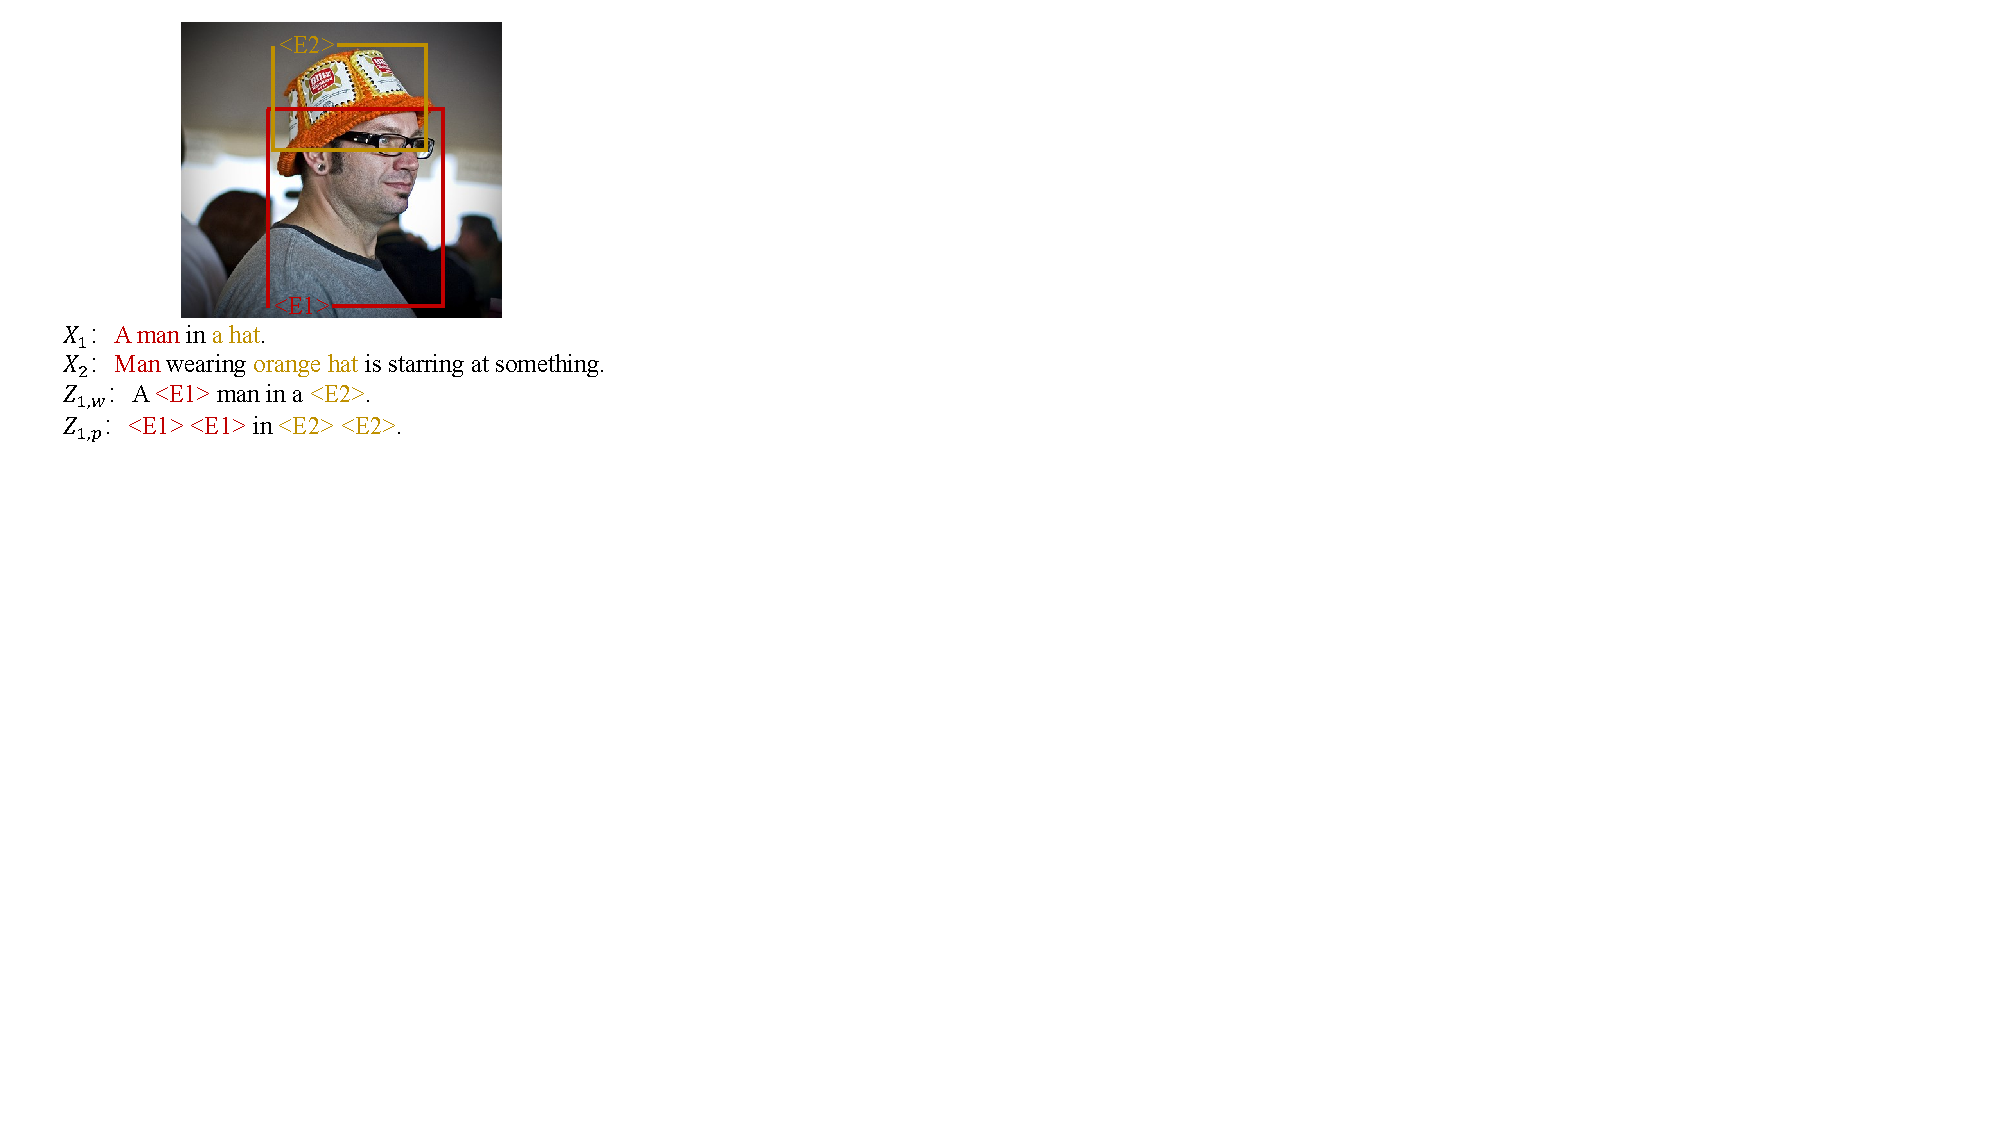
\includegraphics{Img/fig_3_example.pdf}
    \bicaption{词实体与短语实体替换示例}{An example of the word entity and the phrase entity}
    \label{fig:3_example}
\end{figure}
本章所提的句子-图片融合方法将作用于句子中的实体,为此我们以两种语义粒度定义文本实体:

(1){\sffamily 短语实体:}一个短语实体是一个视觉可描述短语,其能够完整的描述一个视觉目标图片。例如,图\ref{fig:3_example}中红框中的人“<E1>”在句子$X_1$中被描述为“A man”。其中,“man”是视觉目标,“A”为“man”的数量修饰词,两个词对于所描述的视觉目标均是有明确意义的。

(2){\sffamily 词实体:}一个词实体是短语实体中的名词实体。对于不同的描述者,视觉目标图像可以被描述为不同的短语。如图\ref{fig:3_example}中,同样是视觉目标“<E1>”,在句子$X_2$中则被描述为“Man”,对视觉目标“<E2>”,$X_1$中描述为“a hat”,在$X_2$中则使用了修饰词“orange hat”。为了消除修饰词所带来的影响,在此方案中只考虑名词作为文本实体。

本章所提的明确的图片信息融合方法,就是将源语言句子中的文本实体直接替换为图片中与文本实体相对应的视觉目标。
由于存在两种文本实体,因此本文设置两种针对句子-图片融合方法的替换规则:短语级替换规则(phrase-level replacement rule,PRR)和词级替换规则(word-level replacement rule,WRR)。在PRR中,将短语内部的所有词逐个用该短语所对应的视觉目标图像替换。例如图\ref{fig:3_example}中,$Z_{1,p}$中的“A”和“man”均被替换为“<E0>”对应的视觉目标。WRR与上述方法相似。如图\ref{fig:3_example}中$Z_{1,w}$仅名词部分(“man”,“hat”)被替换为对应的视觉目标(“<E1>”,“<E2>”)。最后的输入为该退化的句子与视觉目标图像的混合序列。

\subsection{文本重构模型}
\label{sec:3_sentence_reconstruction}
\begin{figure}[!htbp]
    \centering
    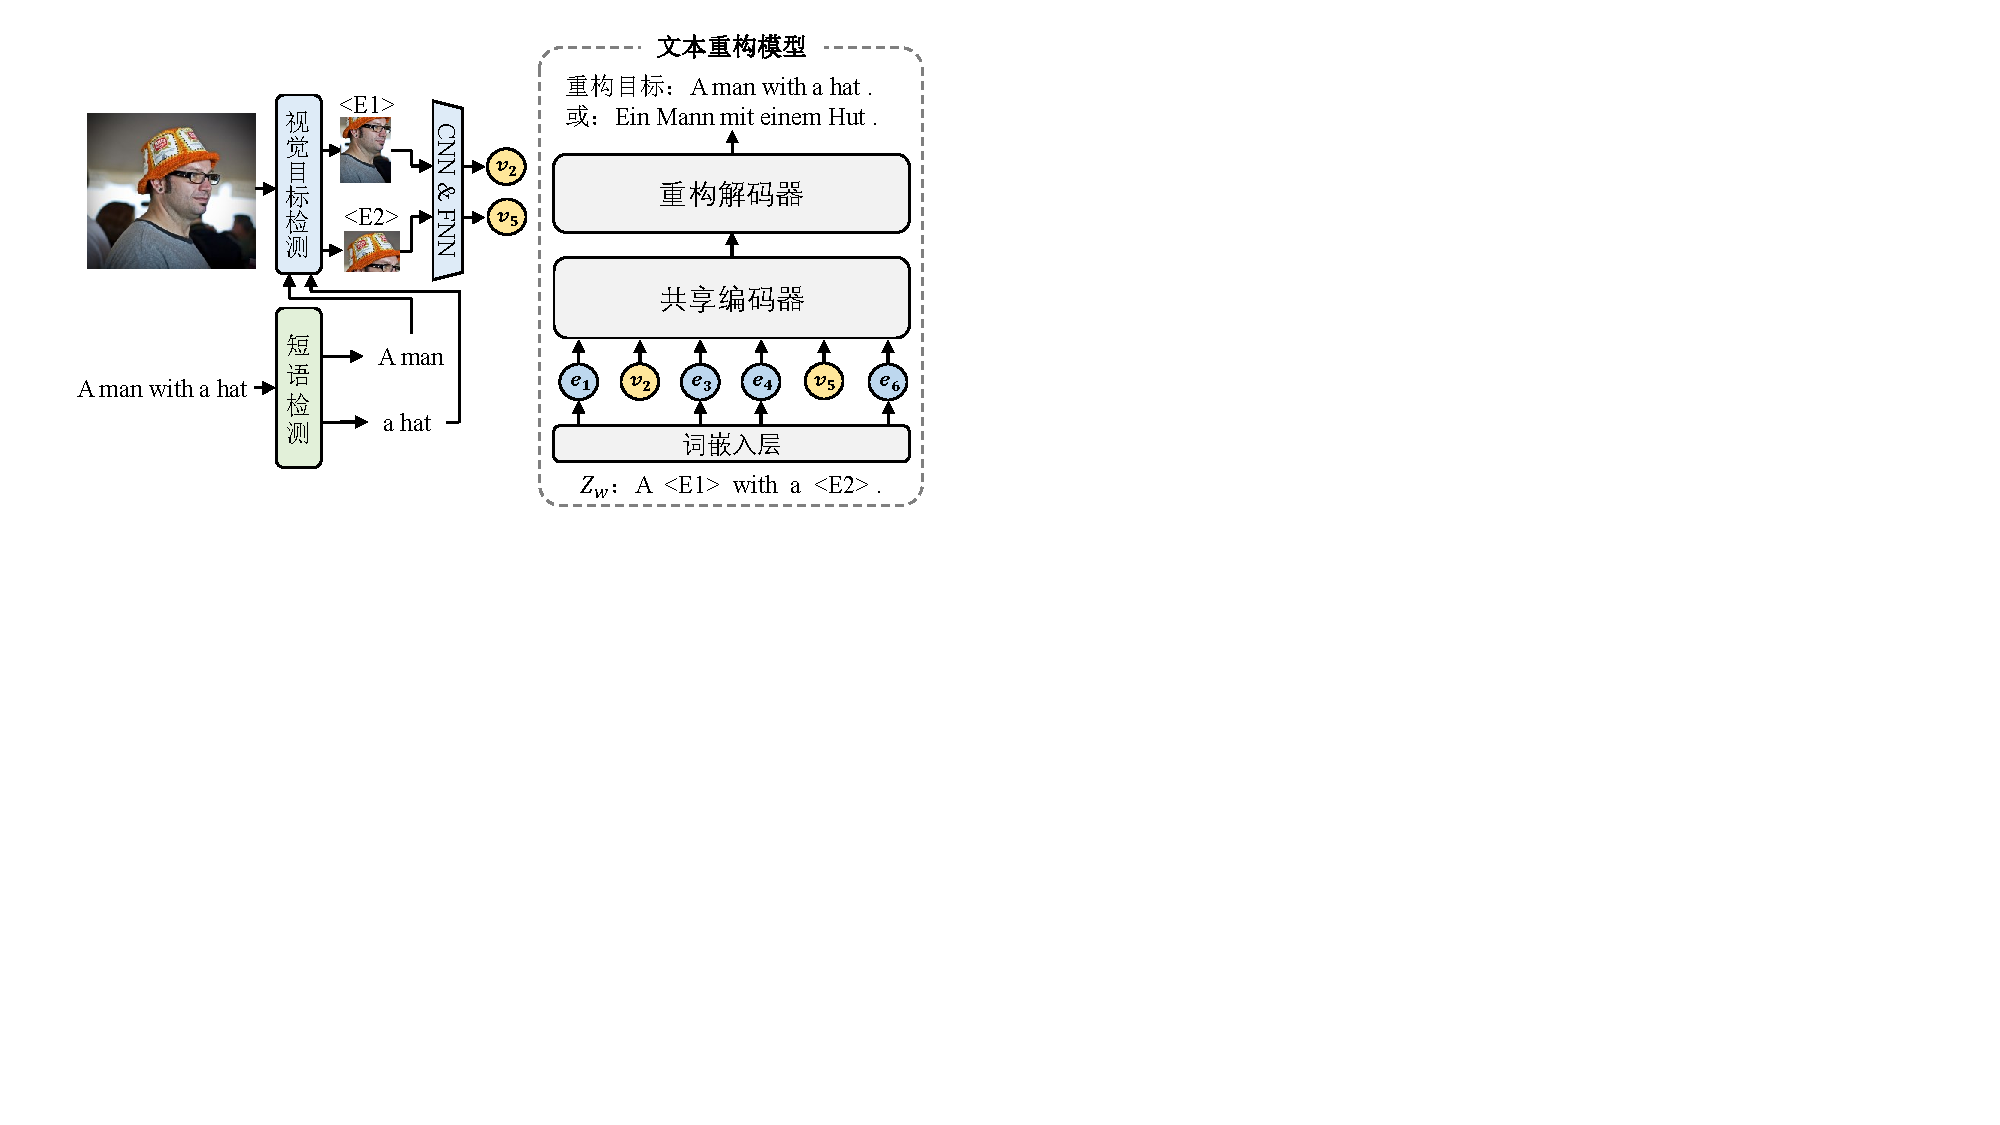
\includegraphics[scale=1.0]{Img/fig_3_reconstruction_model.pdf}
    \bicaption{融合视觉目标信息的文本重构方法}{Text reconstruction by fusing visual object information}
    \label{fig:3_reconstruction_model}
\end{figure}
为了充分利用文本模态和视觉模态的信息,本章设计了文本重构模型使显式跨模态信息融合方法有效。如图\ref{fig:3_reconstruction_model}所示,左侧为利用图\ref{fig:3_entity_extraction}中的方法提取出视觉目标后,再通过预训练的卷积神经网络提取得视觉目标的全局特征,并利用一个前馈神经网络(feedforward neural network, FNN)映射到所需要的维度。图\ref{fig:3_reconstruction_model}右侧的 “文本重构模型”是一个与“翻译模型”相似的序列到序列的生成模型。其多模态输入序列$Z_{w}$是利用WRR得到的退化文本与视觉目标图像的混合序列。该序列的向量表示为$\{\Vector{e_1,v_2,e_3,e_4,v_5,e_6}\}$。重建任务负责从$Z_{w}$重构回原始文本$X=\{x_1,x_2,…,x_N\}$。模型因此可以分别在编码阶段的视觉特征空间和在解码阶段从语言特征空间学习到实体信息。重建模型的训练方式为最小化以下对数似然方程:
\begin{equation}
    \mathcal{L}_R(\theta, \psi)=-\sum_i^N \log p(x_i|x_{<i},Z)
    \label{eq:3_reconstruction_x}
\end{equation}
其中$Z$可以是使用WRR的$Z_{w}$或是采用了PRR的$Z_{p}$,$\theta$为重构模型的编码器参数,$\psi$为重构模型的解码器参数。
考虑到重构目标语言$Y=\{y_1,y_2,\cdots,y_M\}$也是一种可行方案。此时,目标函数调整为:
\begin{equation}
    \mathcal{L}_R(\theta, \psi)=-\sum_j^M \log p(y_j|y_{<j},Z)
    \label{eq:3_reconstruction_y}
\end{equation}

\subsection{与机器翻译相结合}
\label{sec:3_multitask}
图\ref{fig:3_reconstruction_model}中所展示的重构模型与一般的神经机器翻译模型相似,都是基于编码器-解码器结构的端到端生成模型。其中翻译模型的目标函数也与公式\ref{eq:3_reconstruction_x}和公式\ref{eq:3_reconstruction_y}相近:
\begin{equation}
    \mathcal{L}_T(\theta, \phi)=-\sum_j^M \log p(y_j|y_{<j},X)
    \label{eq:3_translation}
\end{equation}
其中$\phi$为神经翻译模型的解码器参数。为了结合重构任务和翻译任务,本章按照文献\cite{37_elliott-kadar-2017-imagination}的方式将两者的目标函数结合:
\begin{equation}
    \mathcal{L}(\theta, \psi, \phi)=\omega L_T(\theta, \phi) + (1-\omega)L_R(\theta, \psi)
    \label{eq:3_combine_sr}
\end{equation}
其中$\omega$是调节多任务训练比例的超参数,即当前批数据用于更新翻译模型参数的概率。相对应的,用于更新文本重构模型参数的概率为$1-\omega$。当前的多任务学习通过共享编码器参数来达到知识迁移的目的。

\subsection{参数共享策略}
\label{sec:3_parameter_sharing}
% 
\begin{figure}[!htbp]
    \centering
    \begin{subfigure}[b]{0.5\textwidth}
      \centering
      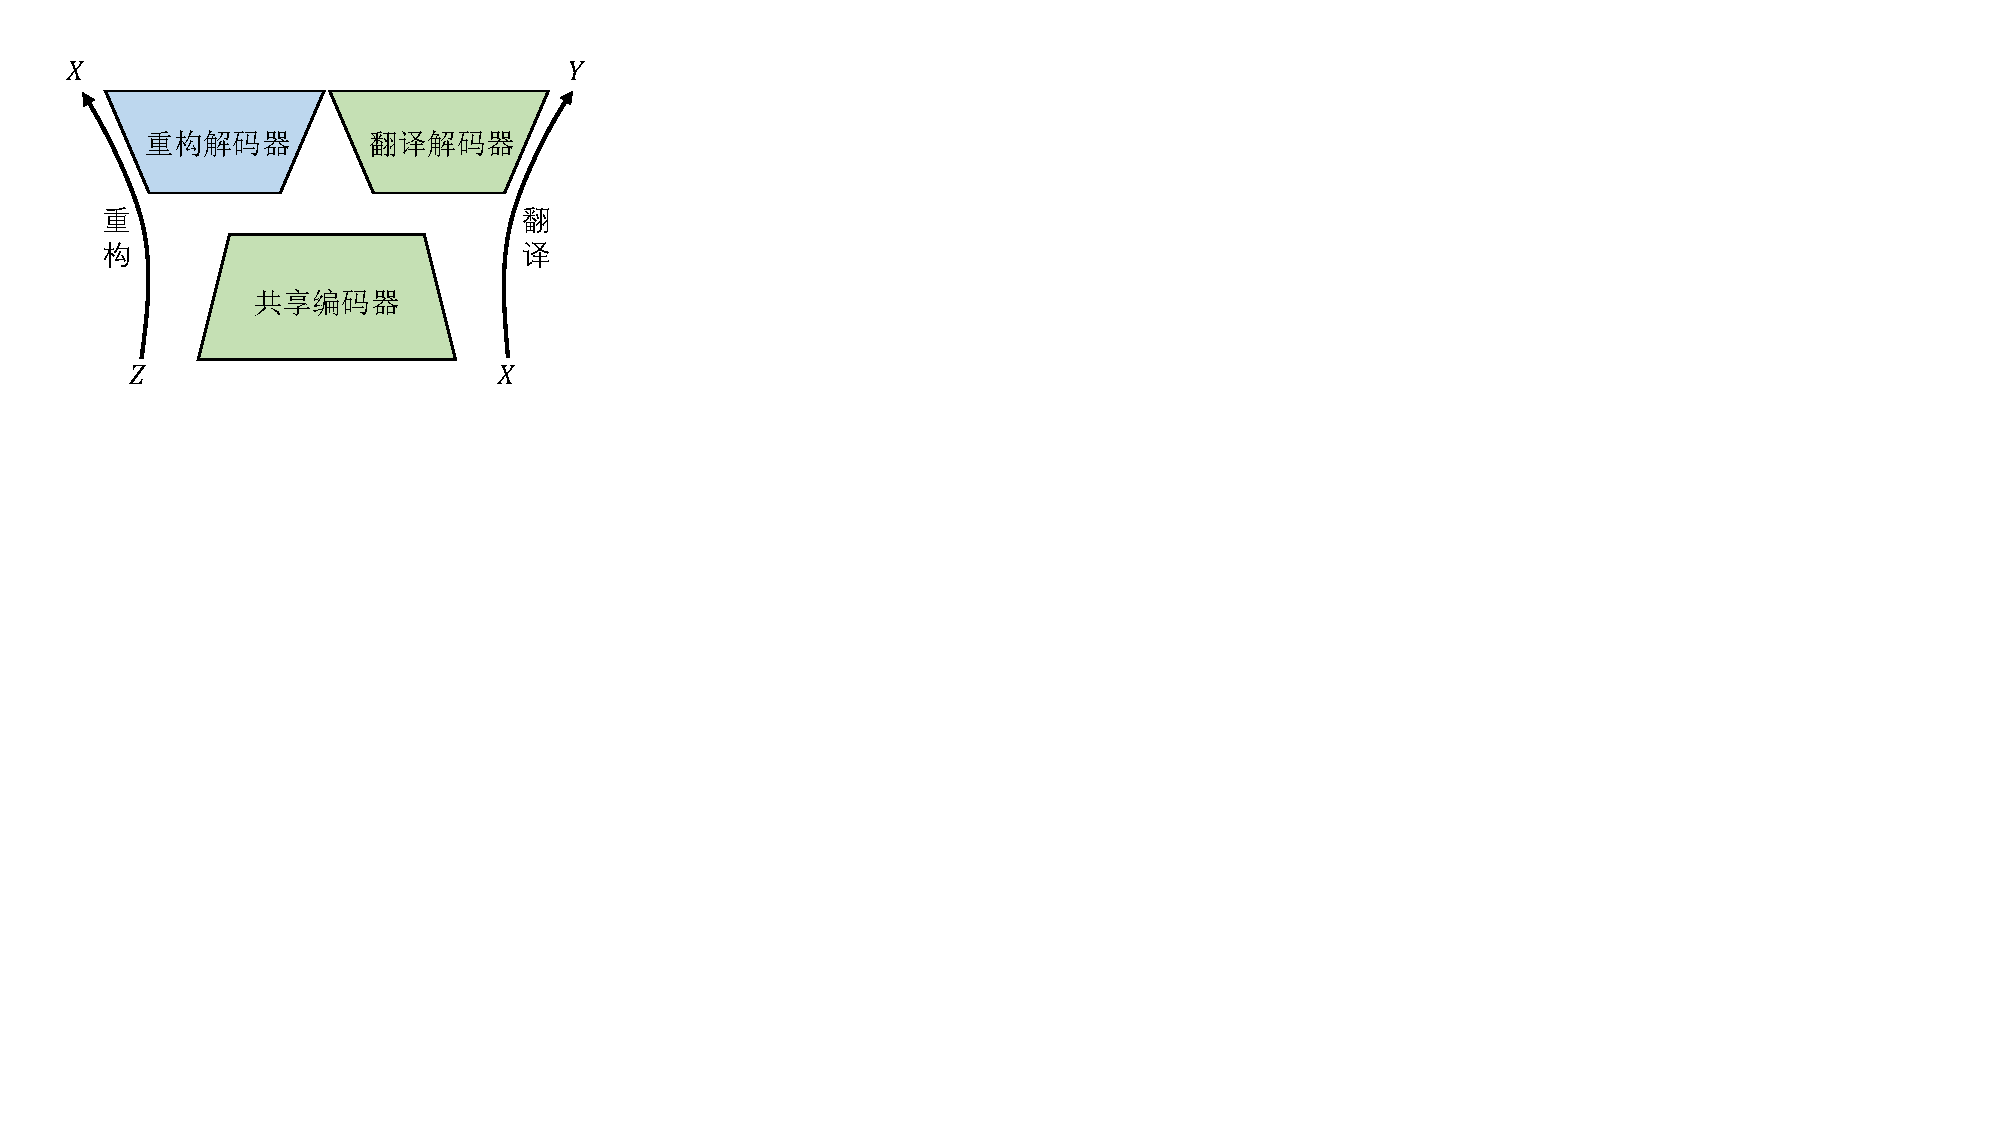
\includegraphics[scale=0.7]{Img/fig_3_sr.pdf}
      \caption{源-独享}
      \label{fig:3_sr}
    \end{subfigure}%
    ~% add desired spacing
    \begin{subfigure}[b]{0.5\textwidth}
      \centering
      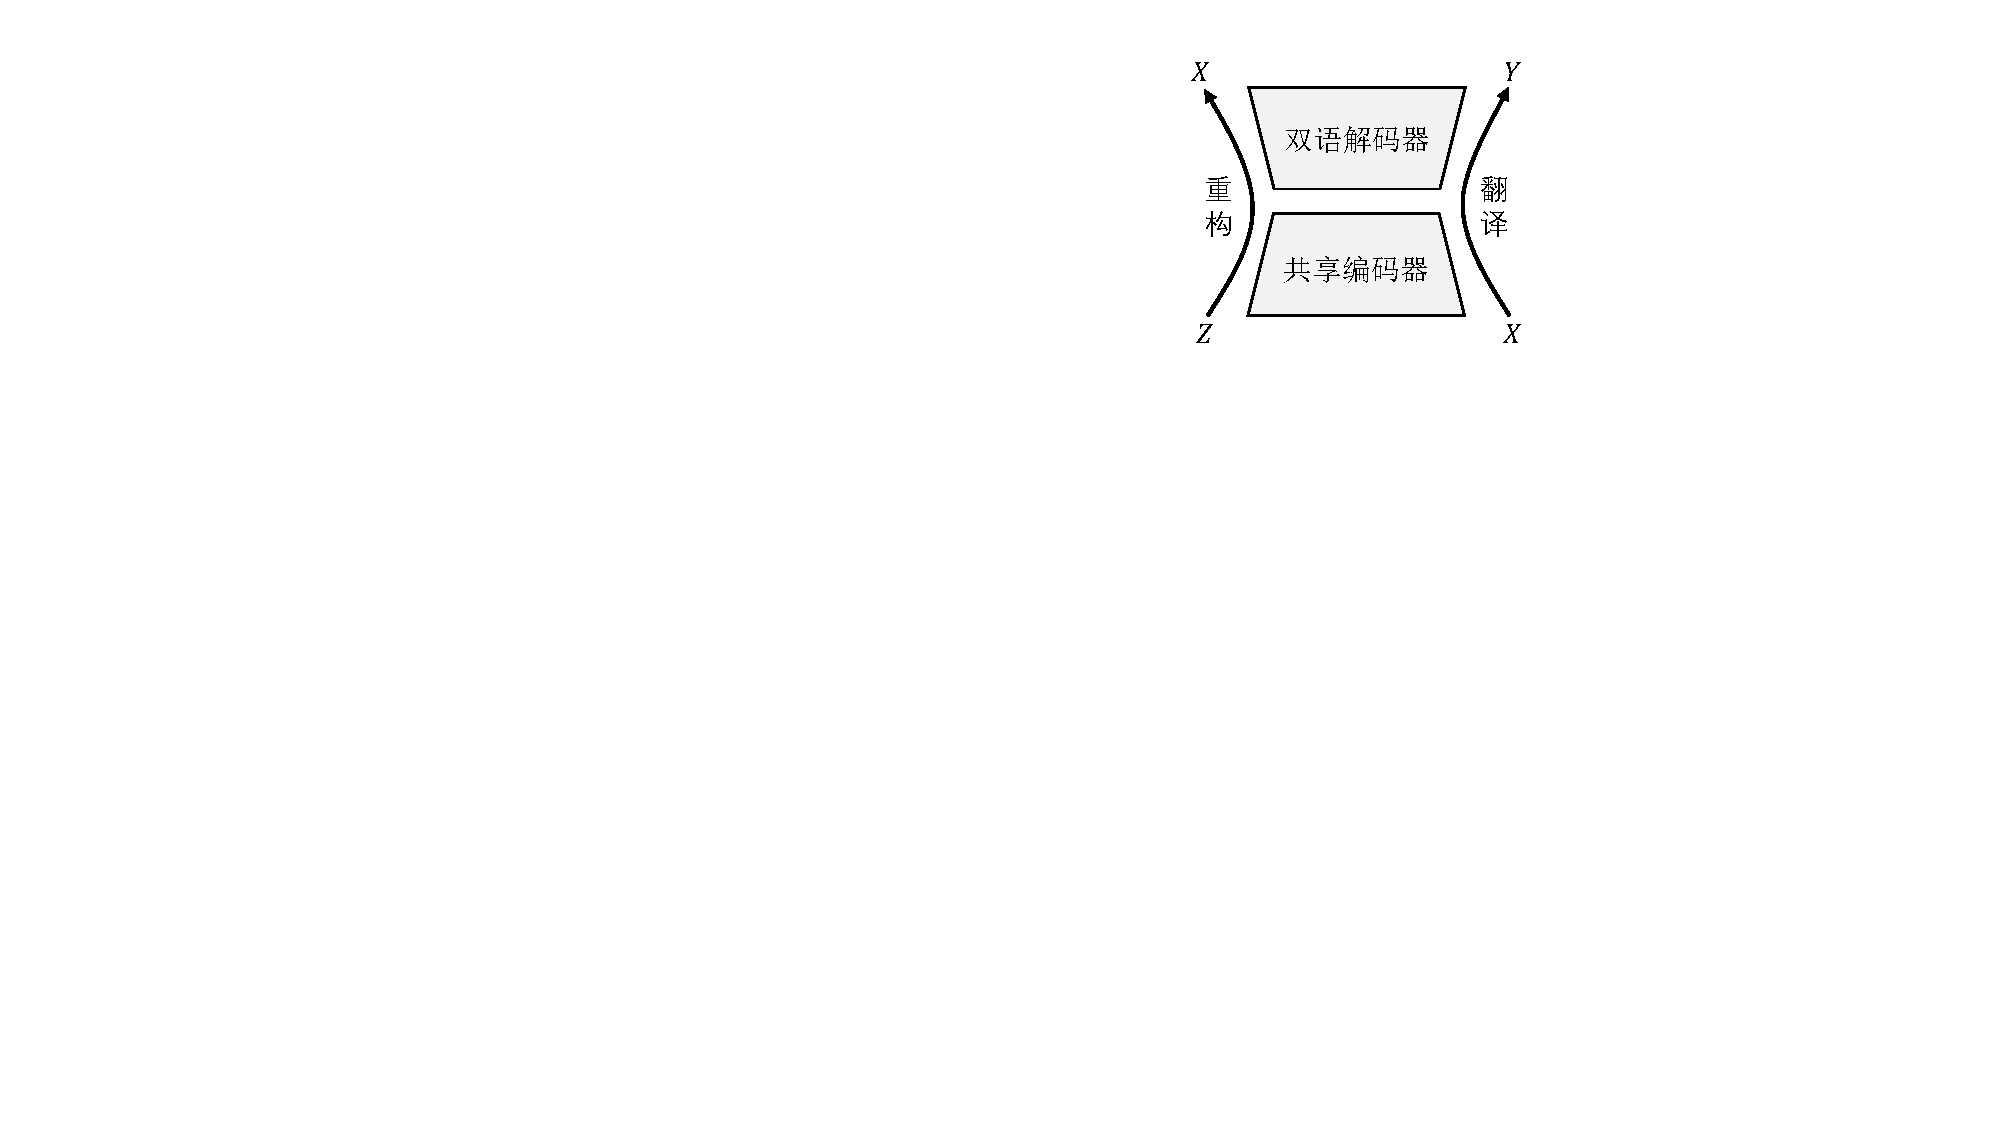
\includegraphics[scale=0.7]{Img/fig_3_ss.pdf}
      \caption{源-共享}
      \label{fig:3_ss}
    \end{subfigure}
    \\% line break
    \begin{subfigure}[b]{0.5\textwidth}
      \centering
      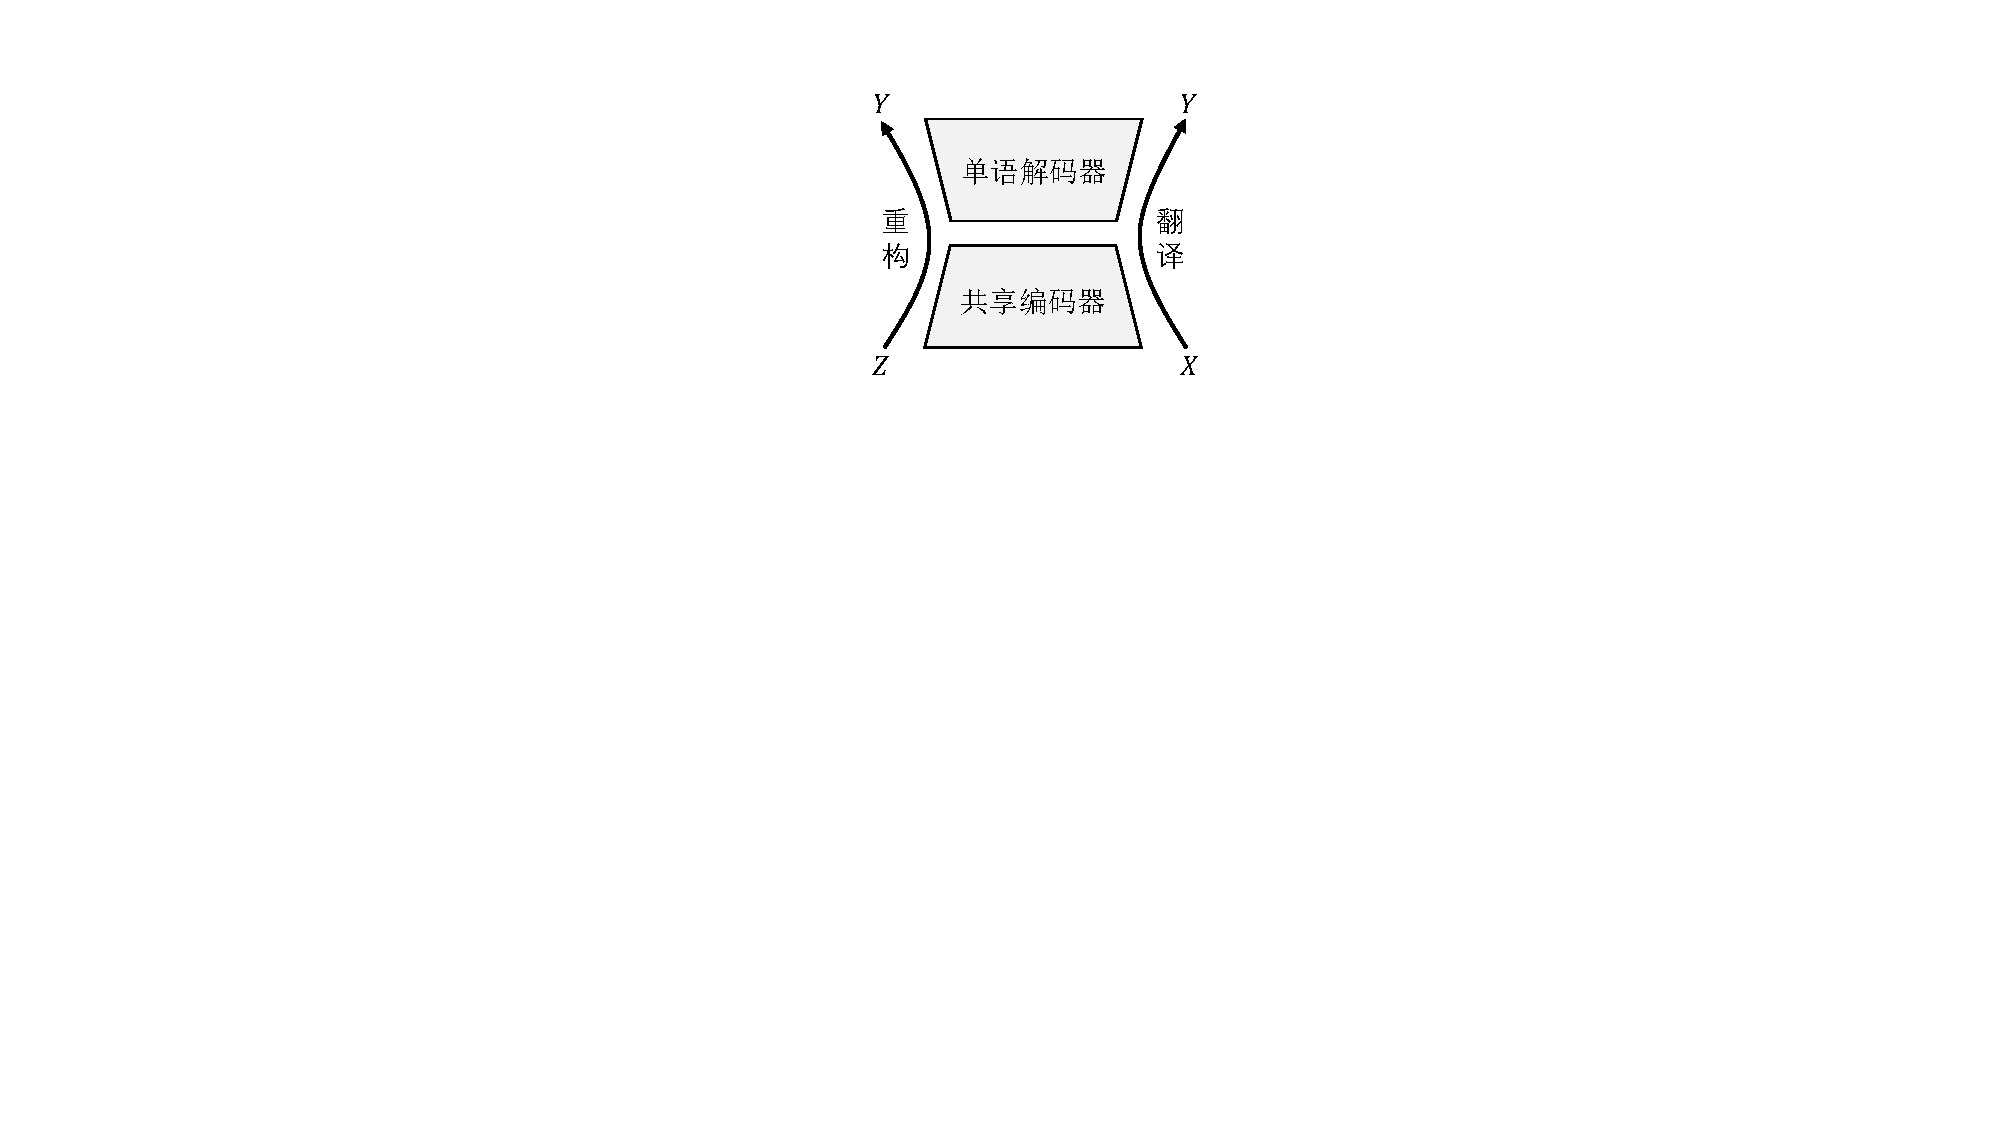
\includegraphics[scale=0.7]{Img/fig_3_t.pdf}
      \caption{目-共享}
      \label{fig:3_t}
    \end{subfigure}%
    \bicaption{重构模型与翻译模型的参数共享方案}{Parameter sharing schemes between reconstruction model and translation model}
    \label{fig:4_fidelity}
\end{figure}
正如前面章节所提到,重构模型与翻译模型在结构上有高度的相似性,因此可以利用参数共享的方法将重构模型学习到的视觉信息融合到翻译模型中,从而达到提升翻译质量的目的。因此,由编码器-解码器结构的灵活性与两种重构目标可组合得到多种参数共享方案。本文采用了以下三种参数共享方案。

(1){\sffamily 独享解码器重构源语言}
\begin{figure}[!htbp]
    \centering
    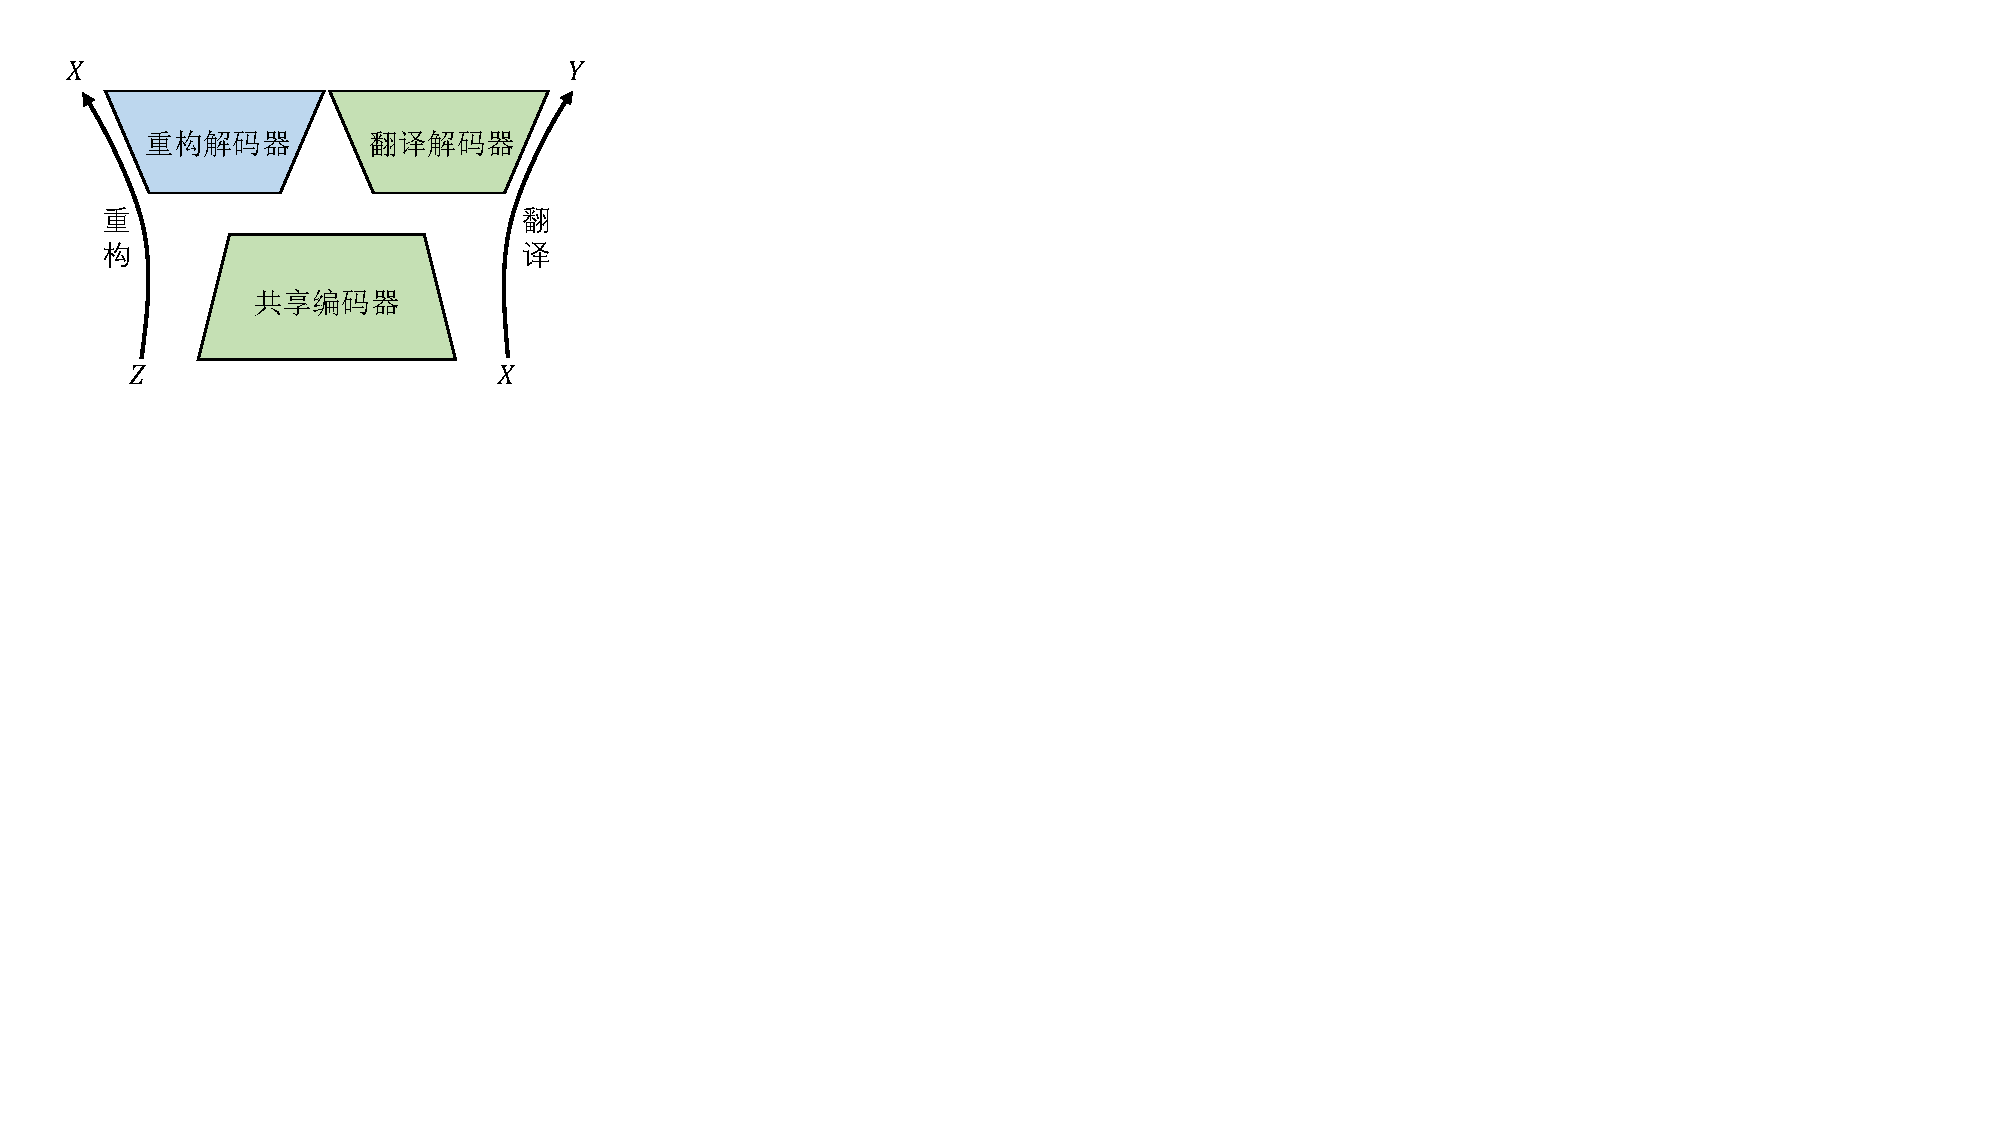
\includegraphics[scale=0.9]{Img/fig_3_sr.pdf}
    \bicaption{独享解码器重构源语言“源-独享”}{Reconstruction for source language with respective decoder}
    \label{fig:3_sr}
\end{figure}

由于视觉信息要在编码的过程中学习特征表示,因此在所有的参数共享策略中,都要包含共享编码器。解码器的参数共享则是可选的。在利用独享解码器重建源语言的策略中,为源语言和目标语言设立独立的解码器,即重构模型和翻译模型的编码器是共享的,解码器参数是独享的。联合目标函数如公式\ref{eq:3_combine_sr},在后面的实验中,本文用“源-独享”表示应用该策略。

(2){\sffamily 共享解码器重构源语言}
\begin{figure}[!htbp]
    \centering
    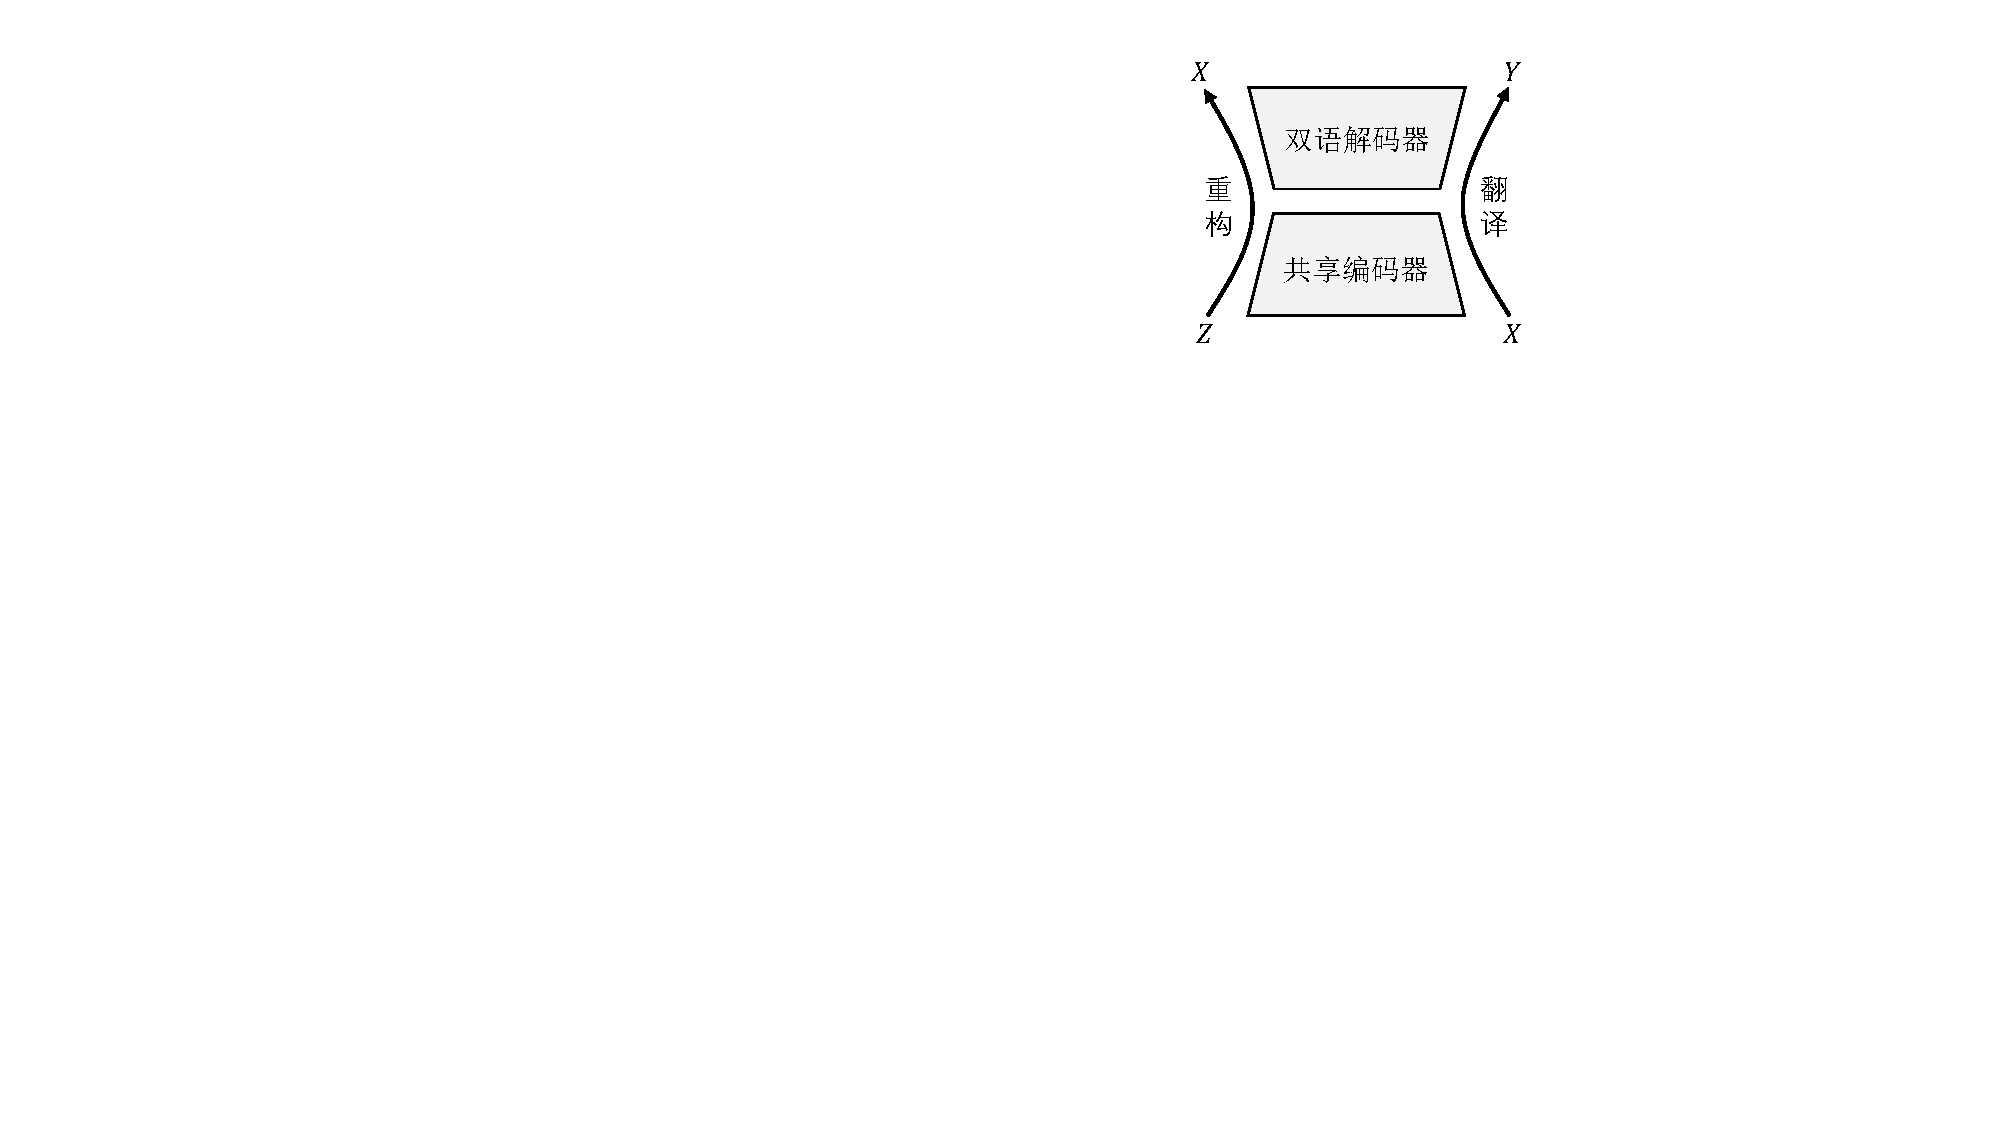
\includegraphics[scale=0.9]{Img/fig_3_ss.pdf}
    \bicaption{共享解码器重构源语言“源-共享”}{Reconstruction for source language with shared decoder}
    \label{fig:3_ss}
\end{figure}

通过融合源语言和目标语言的词表,以及在编码器和解码器之间共享词嵌入层的方式,可以实现重构模型和翻译模型的共享解码器的设置。同时,需要在解码过程目标语言句子输入时,在句首引入一个“识别词”(例如,“<en\_sos>”表示解码到英语,“<de\_sos>”表示解码到德语)用于表示当前解码器用于重构到源语言还是翻译到目标语言。在该设置中,公式\ref{eq:3_combine_sr}中有$\psi=\phi$。这表明该策略中翻译模型和重建模型是全参数共享的。因此,将联合目标函数调整为:
\begin{equation}
    \mathcal{L}(\theta, \phi)=\omega \mathcal{L}_T(\theta, \phi) + (1-\omega)\mathcal{L}_R(\theta, \phi)
    \label{eq:3_combine_ss}
\end{equation}
本文将用“源-共享”代表该参数共享策略。

(3){\sffamily 共享解码器重构目标语言}
\begin{figure}[!htbp]
    \centering
    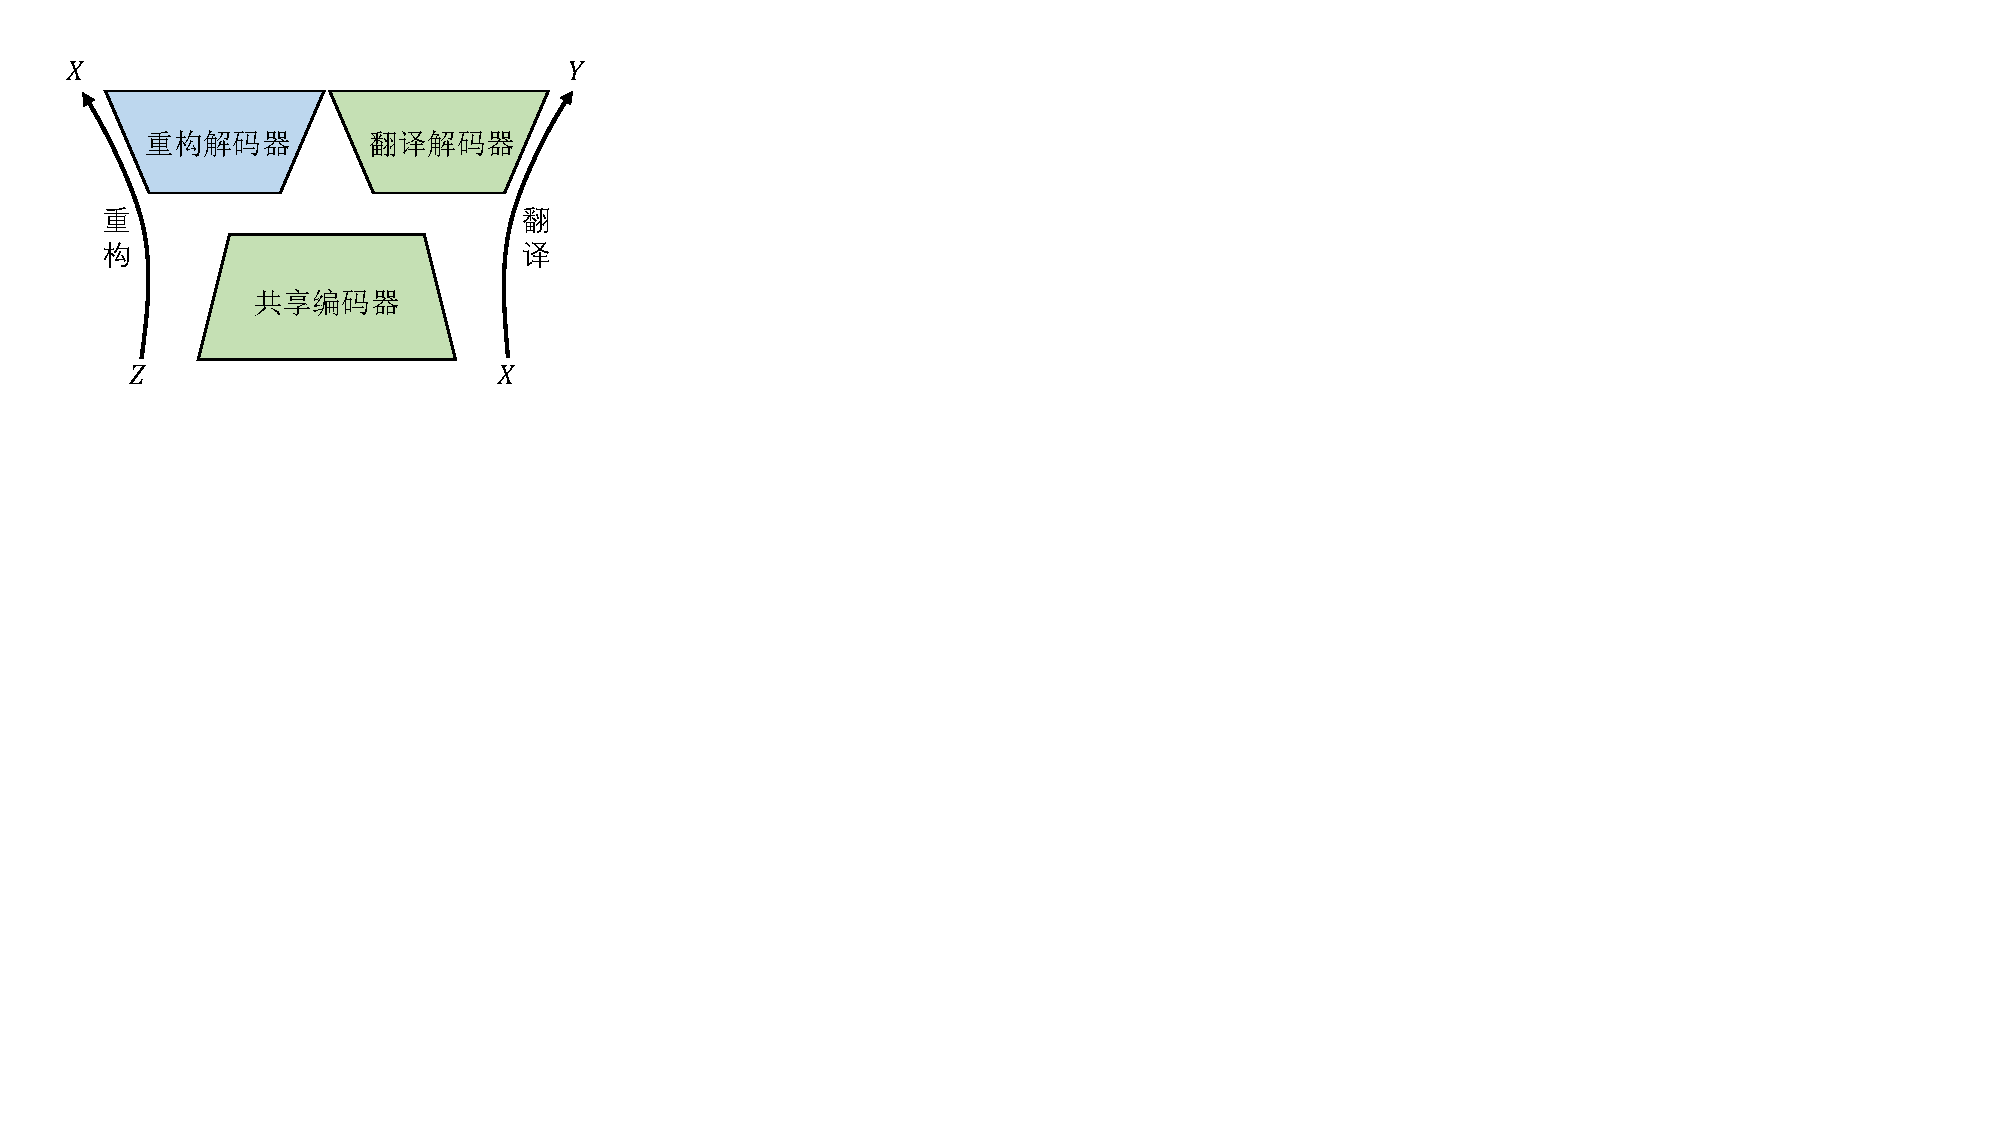
\includegraphics[scale=0.9]{Img/fig_3_sr.pdf}
    \bicaption{共享解码器重构目标语言“目-共享”}{Reconstruction for target language with shared decoder}
    \label{fig:3_t}
\end{figure}

不同于重构源语言,解码器的参数共享策略在重建目标语言的方向上则很容易实现。在该策略中,重构任务的工作方式与一般的MMT模型相似,区别在于输入的文本是退化文本。并且其联合目标函数与公式\ref{eq:3_combine_ss}相同。本文将用“目-共享”来表示该参数共享策略。
\section{实验设置}
为了验证所提方法的有效性,本章在基于循环神经网络和基于Transformer的两种模型上进行了测试。本章选择了融合图片信息的神经机器翻译中最常用的Multi30K\cite{43_elliott-etal-2016-multi30k}数据集的英德翻译进行实验。

\subsection{实验数据}
本文使用图像描述翻译的Multi30K翻译数据集英德翻译对。该数据集每张图片配有一个英文句子和与其对应的德文翻译。该数据集共包含31014张图片,并划分为训练集、验证集和测试集三部分,对应的图片数量分别为:29000,1014和1000。另外,本章还采用了WMT17发布的测试集,包含Multi30K 2017测试集和针对歧义词的ambiguous MSCOCO 2017测试集。这两个测试集同样是每张图片配有一个英文句子和德文翻译,对应的图片数量分别为:1000和461。本文采用Moses SMT\cite{44_koehn-etal-2007-moses}工具包对数据进行分词(tokenization)和归一化(normalization)处理。为了防止对视觉实体与文本实体对应关系的破坏,本文并没有采用双节编码技术\cite{27_sennrich-etal-2016-neural}(byte pair encoding, BPE)或WordPiece\cite{28_DBLP:journals/corr/WuSCLNMKCGMKSJL16}进行分词操作。经过以上预处理后,得到英文词表大小为10209,德文词表为18674,合并后的双语词表大小为27226。

\subsection{实体提取}
\label{sec:3_setup_entity_extraction}
实体提取采用的是\ref{sec:3_entity_extraction}节介绍的方法。其中名词和名词短语提取模块采用的是spaCy\footnote{https://spacy.io/}提供的提取名词短语和词性标注功能。在采用词级替换规则时,所替换的名词占训练集和测试集单词统计量的32.6\%。采用短语级替换规则时,提取的名词短语占单词统计量的45.1\%。同时,我们观察了在词级和短语级替换规则中,所涉及单词的词频情况。两种替换规则下,所涉及单词的词频中位数都是2,这意味着这些词中多数都是低频词。提前视觉目标采用的是\cite{24_DBLP:conf/iccv/YangGWHYL19}所提方法。理论上,只有实体短语可以从图片中检测到,没有在图片中检测到对应视觉目标的名词短语不被列为短语实体。另一种得到对齐的名词短语与视觉目标的方法是使用已标注的数据,Flickr30K Entities\cite{29_DBLP:conf/iccv/PlummerWCCHL15,30_DBLP:journals/ijcv/PlummerWCCHL17}就是标注了图片与文本中实体对应关系的数据集。该数据集与Multi30K高度重合,因此可以直接利用到本章所提方法上。对于从图片中截取到的视觉目标图片,本章利用在ImageNet\cite{31_DBLP:journals/ijcv/RussakovskyDSKS15}上预训练的ResNet-50\cite{32_DBLP:conf/cvpr/HeZRS16}提取2048维的全局特征。

\subsection{基于循环神经网络的模型设置}
\label{sec:3_rnn_setup}
对于基于循环神经网络的翻译模型,本章采用的是带有注意力机制并基于编码器-解码器结构的神经翻译模型\cite{4_luong-etal-2015-effective}。其中,编码器是一个维度维500的单层双向的LSTM,重构模型和翻译模型的解码器都是单层500维的LSTM,词嵌入层的维度同样设置为500。编码器和解码器中的dropout均设置为0.3。模型参数是从$(-0.1,+0.1)$区间的均匀分布中采样初始化的,其中偏置项(bias)初始化为0。训练时采用Adam\cite{34_DBLP:journals/corr/KingmaB14}优化器优化模型参数,学习率设为定值0.002。批数据大小(batch size)为40。最终模型是根据验证集在BLEU4\cite{42_papineni-etal-2002-bleu}上的表现进行选择。在训练过程中,当模型在验证集上的BLEU4值超过10个迭代轮次不再提升,则停止训练并作为最终用于评测的模型。

\subsection{基于Transformer的模型设置}
\label{sec:3_transformer_setup}
对于基于Transformer\cite{5_DBLP:journals/corr/VaswaniSPUJGKP17}的翻译模型,本章将词向量的维度设置为128,隐层状态维度设置为256,自注意力的头数为4,模型编码器和解码器的层数均为4,dropout设置为0.2,批数据大小为2000个单词。区别于基于RNN的模型,Transformer采用的是合并的词表,因此词表大小始终设置为合并词表的大小27226。模型优化采用的是Adam优化器,其中$\beta_1=0.9$,$\beta_2=0.998$,$\epsilon=10^{-9}$。本章与文献\cite{5_DBLP:journals/corr/VaswaniSPUJGKP17}相同采用预热和衰减策略来提高学习率,预热步骤为4000,总训练步骤为80000。训练目标中设置平滑标签(label smoothing)$\epsilon_{ls}=0.1$。测试时,采用了搜索空间$b=4$的柱搜索算法。以上模型参数与文献\cite{33_yin-etal-2020-novel}中的模型设置基本一致。

\subsection{多任务训练}
本章所提方法需要对重建任务和翻译任务采用多任务训练的方式进行模型优化。多任务训练采用的是两个任务随机交替训练的方式,并利用\ref{sec:3_multitask}节中所介绍的超参数$\omega$控制翻译任务的训练概率。因为两个任务所使用数据的比例相同,因此本章设置$\omega=0.5$。

\subsection{对比模型}
基于循环神经网络的模型:
\begin{itemize}
    \item \textbf{NMT:}基于LSTM的纯文本神经翻译模型,其模型配置与\ref{sec:3_rnn_setup}节中的描述保持一致。
    \item \textbf{pRCNNs\cite{35_huang-etal-2016-attention}:}该模型在编码阶段将每个视觉目标特征与源语言句子编码一次,在解码阶段,解码器选择关注与当前解码步骤相关的视觉目标所对应的文本序列。
    \item \textbf{DATT\cite{36_calixto-etal-2017-doubly}:}该模型设置了两个注意力机制模块,其中一个用于关注文本信息,另一个用于关注图片的栅格特征。并设置了一个门控值控制图片信息输入的量。
    \item \textbf{Imagination\cite{37_elliott-kadar-2017-imagination}:}该方法将源语言句子编码后,利用编码后的隐层表示预测输入句子所对应的图片。该方法同样使用了多任务的方式。
    \item \textbf{VMMT\cite{38_calixto-etal-2019-latent}:}该方法中的$ \mathrm{VMMT_C} $与$ \mathrm{VMMT_F} $采用隐变量建模语义信息,在翻译过程中利用视觉信息与文本信息使变分编码器融合跨模态语义。
\end{itemize}

基于Transformer的模型:
\begin{itemize}
    \item \textbf{Transformer:}基于Transformer的纯文本神经机器翻译模型,其模型配置与\ref{sec:3_transformer_setup}节保持一致。
    \item \textbf{DelMMT\cite{39_ive-etal-2019-distilling}:}该模型提出使用推敲做多模态二次接码。在二次解码中融合源语言、目标语言以及视觉信息。
    \item \textbf{MMT-TF\cite{40_yao-wan-2020-multimodal}:}该工作设计了一种多模态注意力模块,该模块需要链接源语言句子的表示和图像特征作为自注意力模块的查询。
    \item \textbf{GAMMT\cite{41_DBLP:journals/corr/abs-2103-08862}:}使用Gumbel-Sigmoid改造注意力机制,帮助翻译模型关注到图片中与文本内容更相关的区域。
    \item \textbf{GMMT\cite{33_yin-etal-2020-novel}:}该模型视源语言句子与图片中的视觉目标为一个多模态图结构,然后利用设计的基于图的跨模态编码器进行编码,最终解码出目标端句子。
\end{itemize}

\section{实验结果}

\subsection{英德翻译结果}

\begin{table}[!htbp]
    \bicaption{基于RNN的神经翻译模型在Multi30K数据集英译德翻译方向的实验结果}{Experiment results of RNN-based NMT on the Multi30K En-De translation pair.}
    \label{tab:3_rnn_ende}
    \centering
    \footnotesize% fontsize
    \setlength{\tabcolsep}{4pt}% column separation
    \renewcommand{\arraystretch}{1.2}%row space 
    \begin{tabular}{cccccccc}
        \hline
        \multicolumn{2}{c}{\multirow{2}{*}{基于RNN}} & \multicolumn{2}{c}{Test2016} & \multicolumn{2}{c}{Test2017} & \multicolumn{2}{c}{MSCOCO} \\ \cline{3-8}
                  & & BLEU        & METEOR      & BLEU         & METEOR        & BLEU         & METEOR   \\ %\hline
    \hline
    \multicolumn{2}{c}{NMT}                                                 & 35.9  & 54.9   & 28.8   & 49.5   & 25.9   & 45.7  \\ %\hline
    \hline
    \multicolumn{2}{c}{pRCNNs \cite{35_huang-etal-2016-attention}}             & 36.5   & 54.1   & -           & -           & -           & -           \\
    \multicolumn{2}{c}{DATT \cite{36_calixto-etal-2017-doubly}}                & 36.5        & 55.0        & -           & -           & -           & -           \\
    \multicolumn{2}{c}{Imagination \cite{37_elliott-kadar-2017-imagination}}   & 36.8   & 55.8   & -           & -           & -           & -           \\
    \multicolumn{2}{c}{$ \mathrm{VMMT_C} $ \cite{38_calixto-etal-2019-latent}} & 37.5   & 55.7   & 26.1   & 45.4   & 21.8   & 41.2   \\
    \multicolumn{2}{c}{$ \mathrm{VMMT_F} $ \cite{38_calixto-etal-2019-latent}} & 37.7   & 56.0   & 30.0   & 49.9   & 25.5   & 44.8   \\ \hline%\hline
                      
    \multirow{3}*{词级} & 
       独享-源   & 37.8           & 56.1           & 30.1           & \textbf{50.3}  & \textbf{27.0}  & \textbf{46.4}  \\
     & 共享-源   & \textbf{38.0}  & 56.2           & 30.3           & 50.1           & 26.1           & 45.6  \\
     & 共享-目    & 36.3           & 55.0           & 28.4           & 48.6           & 25.3           & 44.3  \\ %\hline
    \hline
    \multirow{3}*{短语级} & 
        独享-源  & \textbf{38.0}  & \textbf{56.5}  & 30.2           & \textbf{50.3}  & 26.8           & 46.1  \\
     &  共享-源  & 37.8           & 56.1           & \textbf{30.5}  & 50.1           & 26.0           & 45.5  \\
     &  共享-目  & 36.8           & 55.0           & 29.4           & 49.0           & 26.3           & 45.3  \\ 
        \hline
    \end{tabular}
\end{table}
如\ref{sec:3_entity_replacement}和\ref{sec:3_parameter_sharing}节所述,本章共设置了两种实体替换规则:短语级和词级,以及三种模型参数共享策略:独享解码器重构源语言、共享解码器重构源语言以及共享解码器重构目标语言,并分别以“独享-源”、“共享-源”和“共享-目”作为简化表示,对以上实验配置进行组合后共得到6种模型设置方案。另外,本章还针对以上设置在基于RNN和基于Transformer的翻译模型上都做了实验,并在BLEU4\cite{42_papineni-etal-2002-bleu}和METEOR\cite{46_denkowski-lavie-2014-meteor}两个指标上进行比较。

{\sffamily 基于RNN的模型实验结果:}表\ref{tab:3_rnn_ende}展示了采用基于RNN的神经机器翻译模型在英译德翻译对上的实验结果,其中加粗项表示同列中最好的实验结果。本章与5个融合图片信息的神经机器翻译方法进行了对比,其中pRCNNs和DATT需要在测试过程中为模型输入图片,其它模型包括本章所设计的翻译模型在测试阶段不需要输入图片。该实验结果展示了本章所提方法在纯文本翻译的基础上得到了显著的提升,表明了我们的方法在基于RNN的模型上的有效性。该实验结果同样显示出了6中实验方案的优缺点。对于重构到源语言句子,实验结果中没有表现出采用共享解码器或独享解码器两种配置之间的明显差距,同样在采用词级替换规则或是短语级替换规则的差别也不大。对于重构到目标语言句子,可以观察到其实验结果明显的低于重构到源语言的方案。以上信息表明,为重构任务设置的语言方向是影响本章所提方法实验效果的最大因素。


\begin{table}[!htbp]
    \bicaption{基于Transformer融合图片信息的神经翻译模型在Multi30K数据集英译德翻译方向的实验结果}{Experiment results of Transformer-based NMT fused with image information on the Multi30K En-De translation pair.}
    \label{tab:3_transformer_ende}
    \centering
    \footnotesize% fontsize
    \setlength{\tabcolsep}{4pt}% column separation
    \renewcommand{\arraystretch}{1.2}%row space 
    \begin{tabular}{cccccccc}
        \hline
        \multicolumn{2}{c}{\multirow{2}{*}{基于Transformer}} & \multicolumn{2}{c}{Test2016} & \multicolumn{2}{c}{Test2017} & \multicolumn{2}{c}{MSCOCO} \\ \cline{3-8}
                  & & BLEU        & METEOR      & BLEU         & METEOR        & BLEU         & METEOR   \\ %\hline
    \hline
    \multicolumn{2}{c}{Transformer}                                     & 38.5       & 57.5      & 31.0   & 51.9   & 27.5   & 47.4     \\\hline
    \multicolumn{2}{c}{DelMMT \cite{39_ive-etal-2019-distilling}}          & 38.0            & 55.6           & -           & -           & -           & -             \\
    \multicolumn{2}{c}{MMT-TF \cite{40_yao-wan-2020-multimodal}}           & 38.7            & 55.7           & -           & -           & -           & -             \\
    \multicolumn{2}{c}{GAMMT \cite{41_DBLP:journals/corr/abs-2103-08862}}  & 39.2            & \textbf{57.8}  & 31.4        & 51.2        & 26.9        & 46.0          \\
    \multicolumn{2}{c}{GMMT \cite{33_yin-etal-2020-novel}}                 & \textbf{39.8}   & 57.6           & 32.2        & 51.9        & 28.7        & \textbf{47.6} \\ \hline%\hline
                      
    \multirow{3}*{词级} & 
       独享-源   & 39.7       & 57.5             & \textbf{32.9}    & 51.7             & \textbf{29.1}    & 47.5   \\
     & 共享-源   & 39.4       & \textbf{57.8}    & 32.4             & \textbf{52.1}    & 28.3             & 47.5   \\
     & 共享-目   & 38.7       & 56.2             & 31.0             & 49.6             & 26.5             & 44.9     \\ %\hline
    \hline
    \multirow{3}*{短语级} & 
        独享-源  & 39.3       & 57.4             & 32.7             & 51.8             & 28.7             & 47.5   \\
     &  共享-源  & 39.0       & 57.3             & 32.4             & 51.6             & 28.3             & 47.2   \\
     &  共享-目  & 38.5       & 56.2             & 30.5             & 49.7             & 26.8             & 45.6   \\
        \hline
    \end{tabular}
\end{table}
{\sffamily 基于Transformer的模型实验结果:}表\ref{tab:3_transformer_ende}展示了采用基于Transformer的神经机器翻译模型在英译德翻译对上的实验结果,其中加粗项表示同列中最好的实验结果。5个对比模型中,仅Transformer为纯文本神经机器翻译方法,其它4个模型均需要在测试阶段输入图片。而本章所提方法仅需要在训练阶段输入图片,在测试阶段并不需要。从模型结果的比较结果可以观察到,本章所提方法能够有效地提升基于纯文本的神经翻译模型的翻译准确率,在测试阶段没有输入图片的劣势情况下,本章所提方法依旧与其它方法是可比的。另外,在基于6中模型设置方案的结果比较中可以观察到与基于RNN的模型有相似的现象,即重构的语言方向是影响方法性能的主要因素。该实验结果中还可以发现,词级替换规则的实验结果略胜短语级。


% Table generated by Excel2LaTeX from sheet 'flickr'
\begin{table}[!htbp]
    \bicaption{基于Flickr30K Entities标注实体的实验结果}{Experiment results on the annotated entities provided by Flickr30K entities}
    \label{tab:3_flickr30k_entities}
    \centering
    \footnotesize% fontsize
    \setlength{\tabcolsep}{4pt}% column separation
    \renewcommand{\arraystretch}{1.2}%row space 
    \begin{tabular}{clcccccccc}
    \hline
    \multicolumn{2}{c}{\multirow{2}{*}{模型}} & \multicolumn{4}{c}{基于RNN} & \multicolumn{4}{c}{基于Transformer} \\ \cline{3-10}
    & & \multicolumn{2}{c}{BLEU} & \multicolumn{2}{c}{METEOR} & \multicolumn{2}{c}{BLEU} & \multicolumn{2}{c}{METEOR} \\\hline

    \multirow{3}*{词级} & 
       独享-源   & \textbf{38.0}  & {$\uparrow$ 0.2}  & 56.1  & - 0.0           &  \textbf{39.9}  & {$\uparrow$ 0.2}  & \textbf{58.0}  & {$\uparrow$ 0.3}\\
     & 共享-源   & 38.0  & - 0.0                                    & 55.9  & {$\downarrow$ 0.3}           &  \textbf{39.5}  & {$\uparrow$ 0.1}  & 57.2   & {$\downarrow$ 0.6}        \\
     & 共享-目    & \textbf{36.7}  & {$\uparrow$ 0.4}  & \textbf{55.5}  & {$\uparrow$ 0.5}  &  38.0  & {$\downarrow$ 0.7}           & \textbf{56.9}  & {$\uparrow$ 0.7}\\ \hline
    \multirow{3}*{短语级} & 
       独享-源   & \textbf{38.1}  & {$\uparrow$ 0.1}  & \textbf{56.6}  & {$\uparrow$ 0.1}  &  \textbf{39.4}  & {$\uparrow$ 0.1}  & 57.3   & {$\downarrow$ 0.1}        \\
     & 共享-源   & 37.8  & - 0.0                                    & \textbf{56.2}  & {$\uparrow$ 0.1}  &  \textbf{39.3}  & {$\uparrow$ 0.3}  & 57.1   & {$\downarrow$ 0.2}        \\
     & 共享-目    & \textbf{36.9}  & {$\uparrow$ 0.1}  & \textbf{55.3}  & {$\uparrow$ 0.3}  &  \textbf{38.8}  & {$\uparrow$ 0.3}  & \textbf{56.6}  & {$\uparrow$ 0.4}\\ 
    \hline
    \end{tabular}%
\end{table}%
{\sffamily 基于标注实体的实验结果:}Flickr30K Entities数据集为Multi30K数据集标注了句子中名词短语与图片中视觉目标的对应关系。因此,为了将这些标注数据应用到本章的方法中,仅需要利用词性标注结果识别出这些短语中的名词。表\ref{tab:3_flickr30k_entities}为应用Flickr30K Entities在基于RNN和基于Transformer的模型上的实验结果。加粗项表示相比于表\ref{tab:3_rnn_ende}和表\ref{tab:3_transformer_ende}中相同模型配置下有翻译准确率提升的实验结果。可以观察到,在应用了标注数据后,多数模型都得到了少许翻译准确率的提升。此外还可以观察到,“独享-源”的实验结果普遍要略好于“共享-源”,即重构任务和翻译任务采用各自单独的解码器时效果更佳。

综合以上结果,词级替换规则略优于短语级,应用单独的解码器略优于共享解码器,重构的语言方向影响最大,重构源语言句子带来的翻译准确率提升最多。

\subsection{对抗评估与消融实验}
\label{sec:3_adversarial_ablation}

文献\cite{23_elliott-2018-adversarial}指出,存在部分融合图片信息的神经机器翻译方法所获得的翻译准确率提升与输入的视觉信息相关性不大。在对这部分模型的输入图像进行随机替换后,模型翻译准确率没有表现出显著的变化。因此,检验视觉信息是否在翻译模型中起了作用以及本章所提方法能够是一个必要的过程。可根据本章所提方法的结构假设方法所带来的增益来源于视觉目标中的视觉信息,多任务学习策略,以及模型的抗噪声能力。为此,设计了以下实验来验证方法的有效性:

(1){\sffamily 噪声输入:}在该方案中,我们应用两种噪声输入方法:随机图片和随机单词。随机图片就是在数据集中随机选取图片,输入错误的视觉目标。随机单词是将原本替换为视觉目标的位置替换为在词表中随机选择的词。

(2){\sffamily 掩码输入:}在该方案中,输入序列中视觉目标的位置替换为一个特殊的单词“<mask>”,此时的重构模型类似于一个掩码语言模型(masked language model),区别在于重构模型采用了序列解码的方式。

% Table generated by Excel2LaTeX from sheet 'ablation'
\begin{table}[!htbp]
    \bicaption{对抗评估与消融实验}{Adversarial evaluation and ablation study}
    \label{tab:3_adversarial_ablation}
    \centering
    \footnotesize% fontsize
    \setlength{\tabcolsep}{4pt}% column separation
    \renewcommand{\arraystretch}{1.2}%row space 
    \begin{tabular}{clcccc}
    \hline
    \multicolumn{2}{c}{\multirow{2}{*}{基于RNN}} & \multicolumn{4}{c}{BLEU} \\ \cline{3-6}
     &        & 原图片          & 随机图片           & 随机单词            & 掩码 \\
    \hline
    \multirow{3}*{词级} & 
       独享-源 & \textbf{37.8}  & 37.4              & 37.1             & \underline{36.8} \\%              & 37.5 \\ 
     & 共享-源 & \textbf{38.0}  & 37.8              & \underline{37.6} & \underline{37.6} \\%              & 38.2 \\
     & 共享-目 & \textbf{36.3}  & \textbf{36.3}     & \underline{35.0} & 35.6 \\\hline%              & 37.4 \\ \hline
    \multirow{3}*{短语级} & 
       独享-源 & \textbf{38.0}  & 37.2              & 37.3             & \underline{36.9} \\%              & 37.2 \\
     & 共享-源 & \textbf{37.8}  & \underline{37.5}  & 37.6             & 37.6 \\%              & 38.2 \\
     & 共享-目 & \textbf{36.8}  & 36.2              & 35.9             & \underline{35.3} \\%              & 37.3 \\ 
    \hline
    \end{tabular}%
\end{table}%
将该对抗评估方案应用于基于RNN的模型上,得到结果如表\ref{tab:3_adversarial_ablation}所示,加粗项代表同一配置的模型中的性能最佳,下划线项代表最差。从表\ref{tab:3_adversarial_ablation}可以观察到,输入为原图像的模型均取得了最佳的性能,同时两组对抗实验均表现出较差的结果。采用掩码输入的方式整体效果最差,说明多任务的方式带来的增益效果并不是主要因素。该实验结果表明本章所提方法确实能够捕捉到视觉信息,从而为翻译准确率带来提升。

\subsection{重构模型的对抗评估与消融实验}
\label{sec:3_adversarial_ablation_rec}

% Table generated by Excel2LaTeX from sheet 'ablation'
\begin{table}[!htbp]
    \bicaption{重构模型的对抗评估与消融实验}{Adversarial evaluation and ablation study for reconstruction model}
    \label{tab:3_adversarial_ablation_rec}
    \centering
    \footnotesize% fontsize
    \setlength{\tabcolsep}{4pt}% column separation
    \renewcommand{\arraystretch}{1.2}%row space 
    \begin{tabular}{clcccc}
    \hline
    \multicolumn{2}{c}{\multirow{2}{*}{基于RNN}} & \multicolumn{4}{c}{BLEU} \\ \cline{3-6}
     &        & 原图片          & 随机图片           & 随机单词            & 掩码 \\
    \hline
    \multirow{3}*{词级} & 
       独享-源 & \textbf{44.5}  & 43.9              & 42.4              & \underline{40.0} \\
     & 共享-源 & \textbf{45.2}  & 43.6              & \underline{2.6}   & 25.1 \\
     & 共享-目 & \textbf{16.6}  & 15.8              & \underline{15.7}  & 16.0 \\\hline%              & 37.4 \\ \hline
    \multirow{3}*{短语级} & 
       独享-源 & \textbf{35.4}  & \underline{23.7}  & 26.5              & 24.9 \\
     & 共享-源 & \textbf{35.2}  & 27.6              & \underline{2.1}   & 24.2 \\
     & 共享-目 & \textbf{13.3}  & 10.6              & \underline{10.3}  & 10.5 \\ 
    \hline
    \end{tabular}%
\end{table}%
本节还进一步地为重构模型设置了对抗评估与消融实验,如表\ref{tab:3_adversarial_ablation_rec}所示为实验结果。这些结果进一步支持了在翻译模型上得到的结论,表明重构任务是有效的。 另一方面,图片信息带来的增益效果似乎受到输入的视觉特征比例的影响。正如我们所看到的,短语级替换方案似乎扩大了我们的模型和对抗模型之间的质量差异。这表明在重构模型中虽然文本信息越少重构的质量越差,但视觉信息的作用却越大。

词级替换规则和短语级替换规则之间的巨大性能差距是由\ref{sec:3_entity_replacement}小节中提到的修饰词难以预测引起的。从视觉对象中预测修饰词是极其困难的。这就是为什么短语级替换模型获得比单词级低得多的重构BLEU值的原因。除了修饰词外,词实体也包含在短语实体中。这些词实体确保了短语级方案获得与词级相似的翻译性能,因此两者虽然在重构的结果上有较大的差异,但在翻译的结果上没有太大的差别。

\subsection{实体词翻译分析}
本节,我们将进一步分析,探索出实体融合与文本重构能够有效提升翻译准确率的原因。本章所提方法具有明确的作用目标,因此我们认为方法的有效性主要来源于该方法能够提升实体词的翻译准确率。为此我们需要进行以下步骤:

(1)首先,我们将测试集中的词分为两类:实体词和非实体词。实体词就是使用替换规则得到的词。因此短语级替换规则包含了更多的词,而这些多出部分的词大部分为助词或修饰词,且这些助词与修饰词也大量存在于非实体词的词表内,所以为了尽量将实体词与非实体词的词表划分开,本章仅针对词级替换规则进行分析。这样,实体词就是名词实体,非实体词为语料中的其它词。

(2)然后,我们需要测试出模型的翻译结果中,实体词与非实体词的翻译准确率。该操作需要将输入的源语言句子与目标语言句子进行词级别的双语对齐。为此,本章采用fast-align\cite{45_dyer-etal-2013-simple}工具对齐双语句子。为了得到更准确的对齐结果,需要将测试语料与训练数据拼接后训练一个好的对齐模型。将源语言句子与语料提供的译文进行对齐的结果作为标准答案,源语言句子与模型解码的结果对齐后参照标准答案统计实体词和非实体词的召回率作为两者的翻译准确率。

(3)方法所带来的提升,应该体现在该方法与对应的纯文本基线模型的比较上。为此,还需要将方法的实体词或非实体词准确率减去对应纯文本基线模型的准确率,就得到了实体词与非实体词继续该方法的提升结果,我们称之为增量差(increment difference)。最后再在方法之间进行横向比较增量差,就可以对比出那些方法为实体词或非实体词带来的提升更多。

\begin{figure}[!htbp]
    \centering
    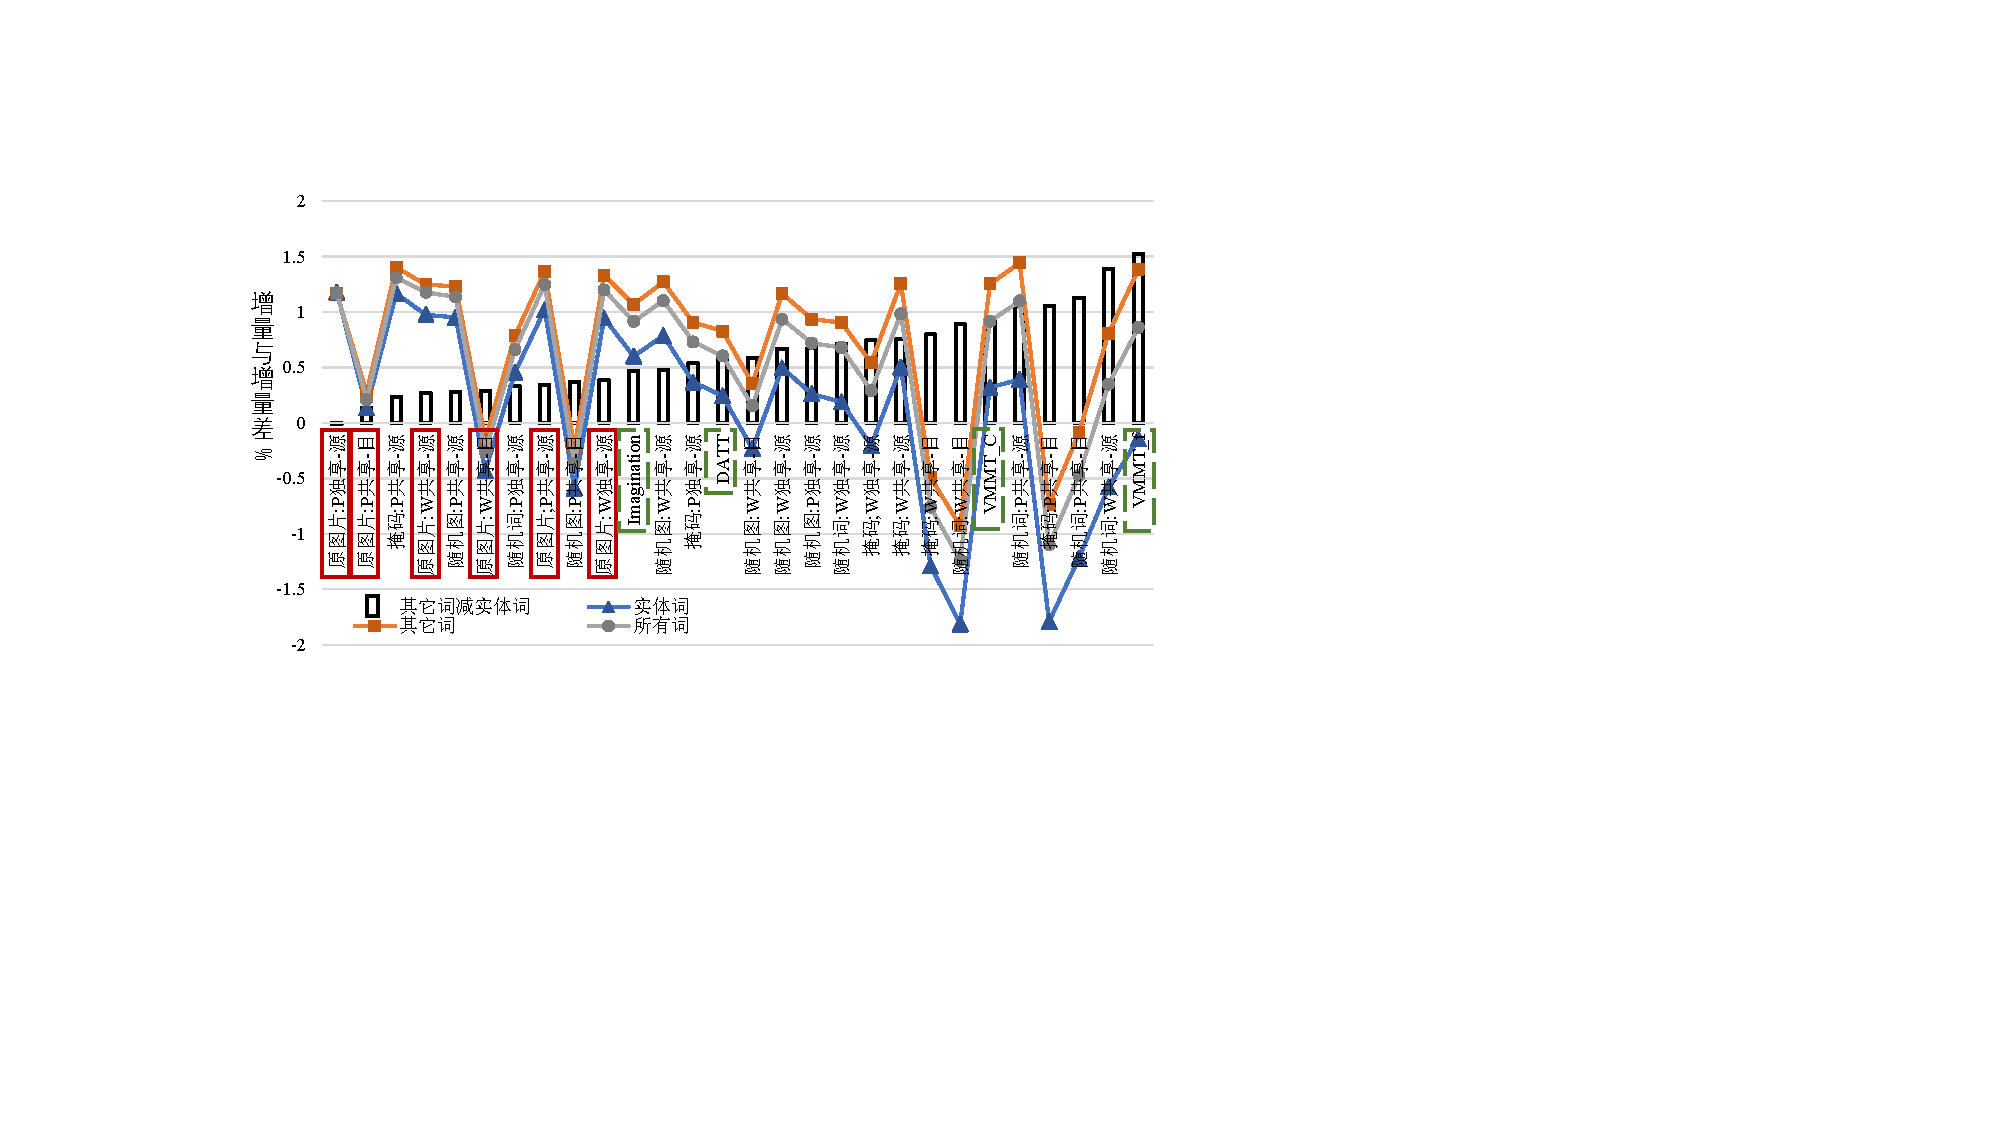
\includegraphics[scale=0.9]{Img/fig_3_analysis.pdf}
    \bicaption{实体词翻译准确率增量与增量差分析}{Accuracy increment and incremental difference analysis of entity words}
    \label{fig:3_analysis}
\end{figure}
由于基于RNN的方法提供的代码比较全,所以我们选择在基于RNN的模型上进行比较。该结果需要每个方法提供模型的解码结果以及对应的纯文本基线模型的解码结果。比较的结果基于4种类型方法:6个本章的基于RNN的方法,12个\ref{sec:3_adversarial_ablation}小节中的对抗模型,6个\ref{sec:3_adversarial_ablation}小节中的掩码模型,以及4个\ref{tab:3_rnn_ende}表中的对比模型。实验结果中,我们同样测量了“所有词”的准确率,即不区分实体词或非实体词的准确率。实验结果如图\ref{fig:3_analysis}所示,其中横轴代表不同的翻译系统,纵轴为增量差,蓝线代表实体词的增量值,红线代表非实体词的增量值,灰线代表所有词的增量值,直方图代表非实体词与实体词的增量值之差。

{\sffamily 本章所提方法:}图中实线框内的方法为本章所提方法。图中一个值得注意的结果是,几乎所有的方法非实体词的增量值都大于实体词的增量值。正如\ref{sec:3_setup_entity_extraction}小节所提到,多数实体词都是低频词,这导致模型更难学习这部分词的表示,所以当一个方法对神经翻译模型带来增益时,对所有词的提升是普遍现象,该提升也主要表现在非实体词上,对实体词的提升就要看各类方法的特点了。从图中直方图可以看到,本章所提方法的增量值之差普遍偏小,这说明该方法能够拉小了实体词与非实体词之间增量差的差距,也就是为实体词带来的翻译准确率提升更多。

{\sffamily 本文的对抗与消融方法:}从图中可以看出对抗评估和消融实验中所使用的模型普遍得到较高的实体词与非实体词的增量值之差。没有证据表明降噪能力或多任务掩码方案能够帮助翻译中的实体词。这进一步证明了本章所提方法能够从视觉目标中提取有价值的视觉信息。

{\sffamily 对比模型方法:}DATT、$ \mathrm{VMMT_C} $、$ \mathrm{VMMT_F} $以及Imagination并没有明显地表现出降低实体词与非实体词的增量值之差的能力,以上整体的对比结果表明本章所提的显式跨模态信息融合方法能够有效地提升实体词的翻译准确率。

\subsection{样例分析}
\begin{figure}[!htbp]
    \centering
    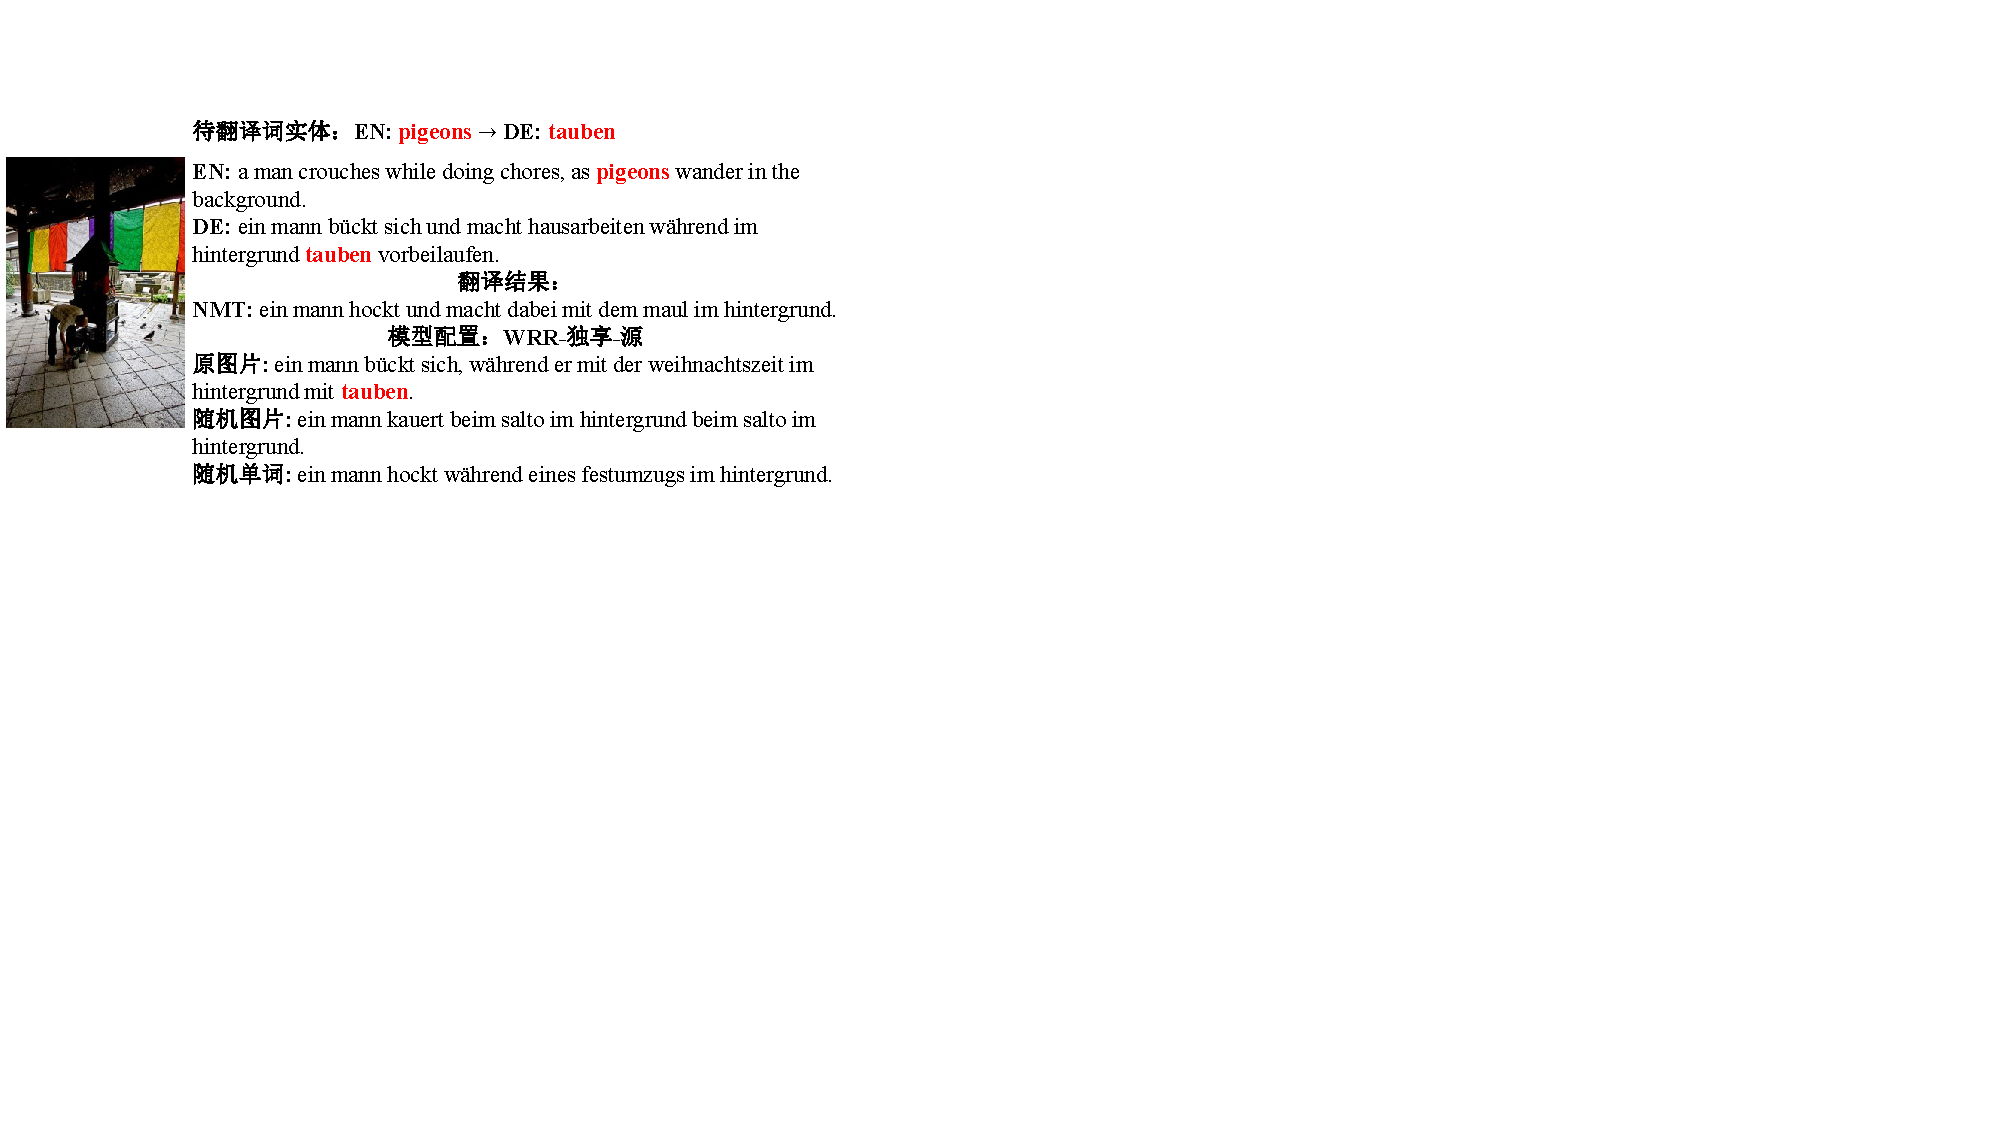
\includegraphics[scale=1.0]{Img/fig_3_case_1.pdf}
    \bicaption{实体词翻译准确率增量与增量差分析}{Accuracy increment and incremental difference analysis of entity words}
    \label{fig:3_case_1}
\end{figure}
\begin{figure}[!htbp]
    \centering
    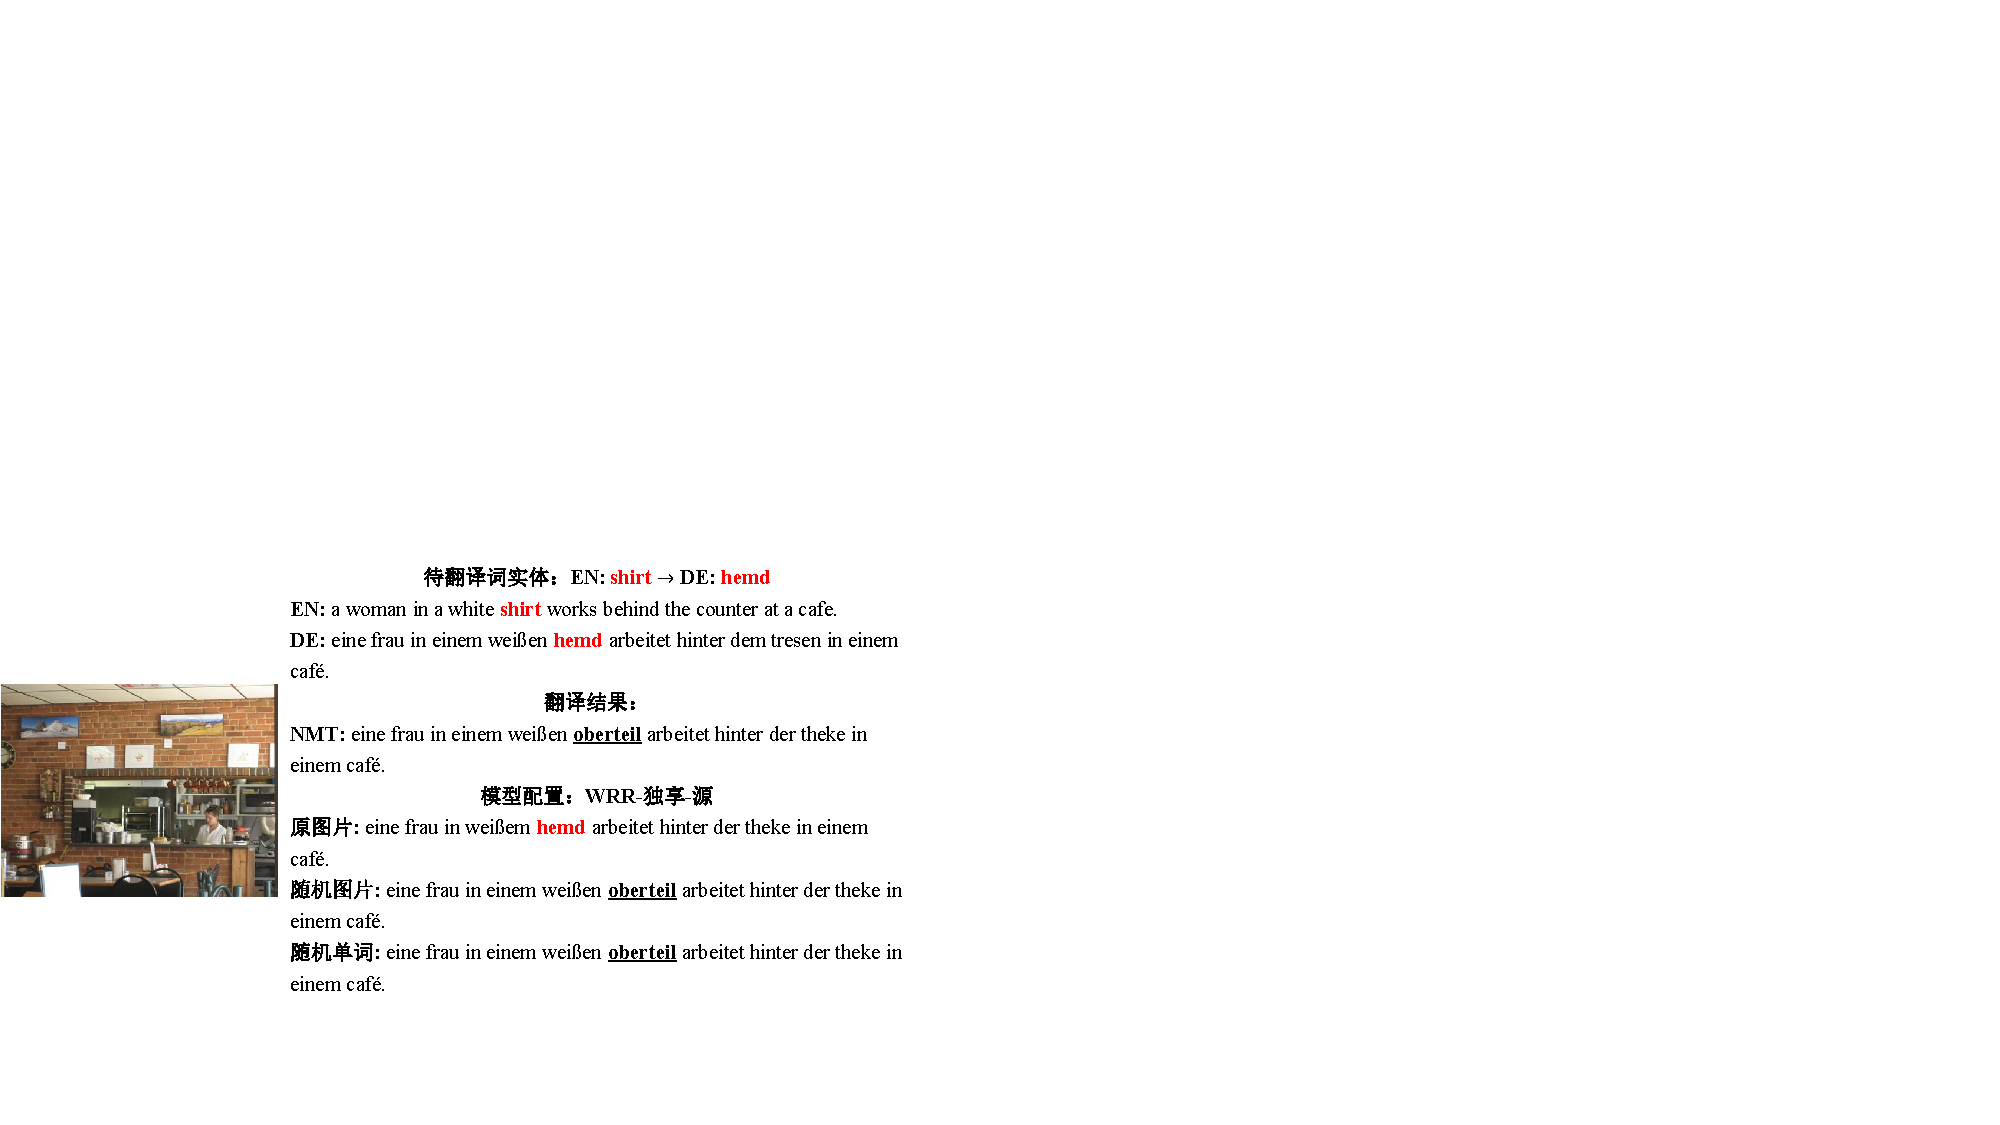
\includegraphics[scale=1.0]{Img/fig_3_case_2.pdf}
    \bicaption{实体词翻译准确率增量与增量差分析}{Accuracy increment and incremental difference analysis of entity words}
    \label{fig:3_case_2}
\end{figure}
\begin{figure}[!htbp]
    \centering
    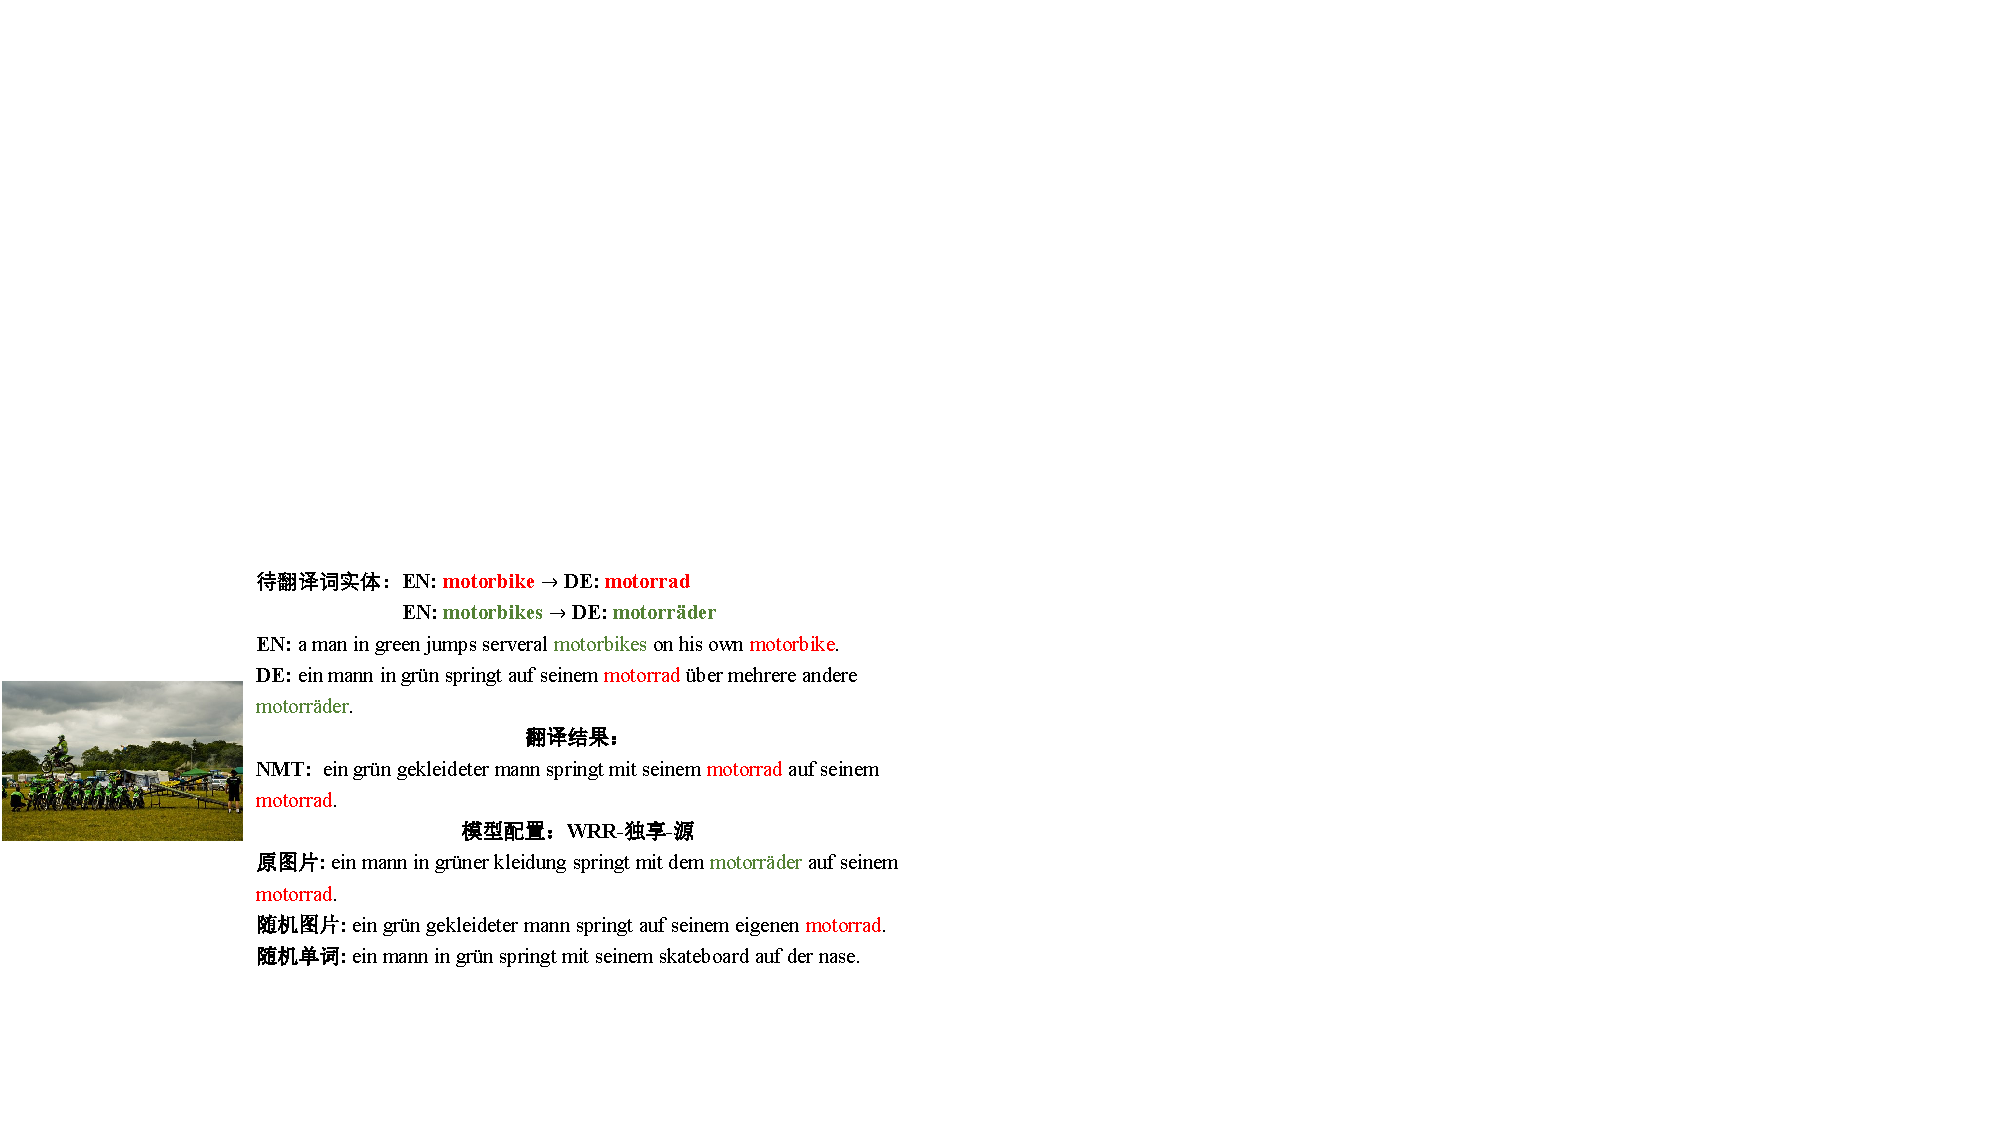
\includegraphics[scale=1.0]{Img/fig_3_case_3.pdf}
    \bicaption{实体词“motorbike”的翻译样例}{Translation example for the entity word "motorbike"}
    \label{fig:3_case_3}
\end{figure}
\begin{figure}[!htbp]
    \centering
    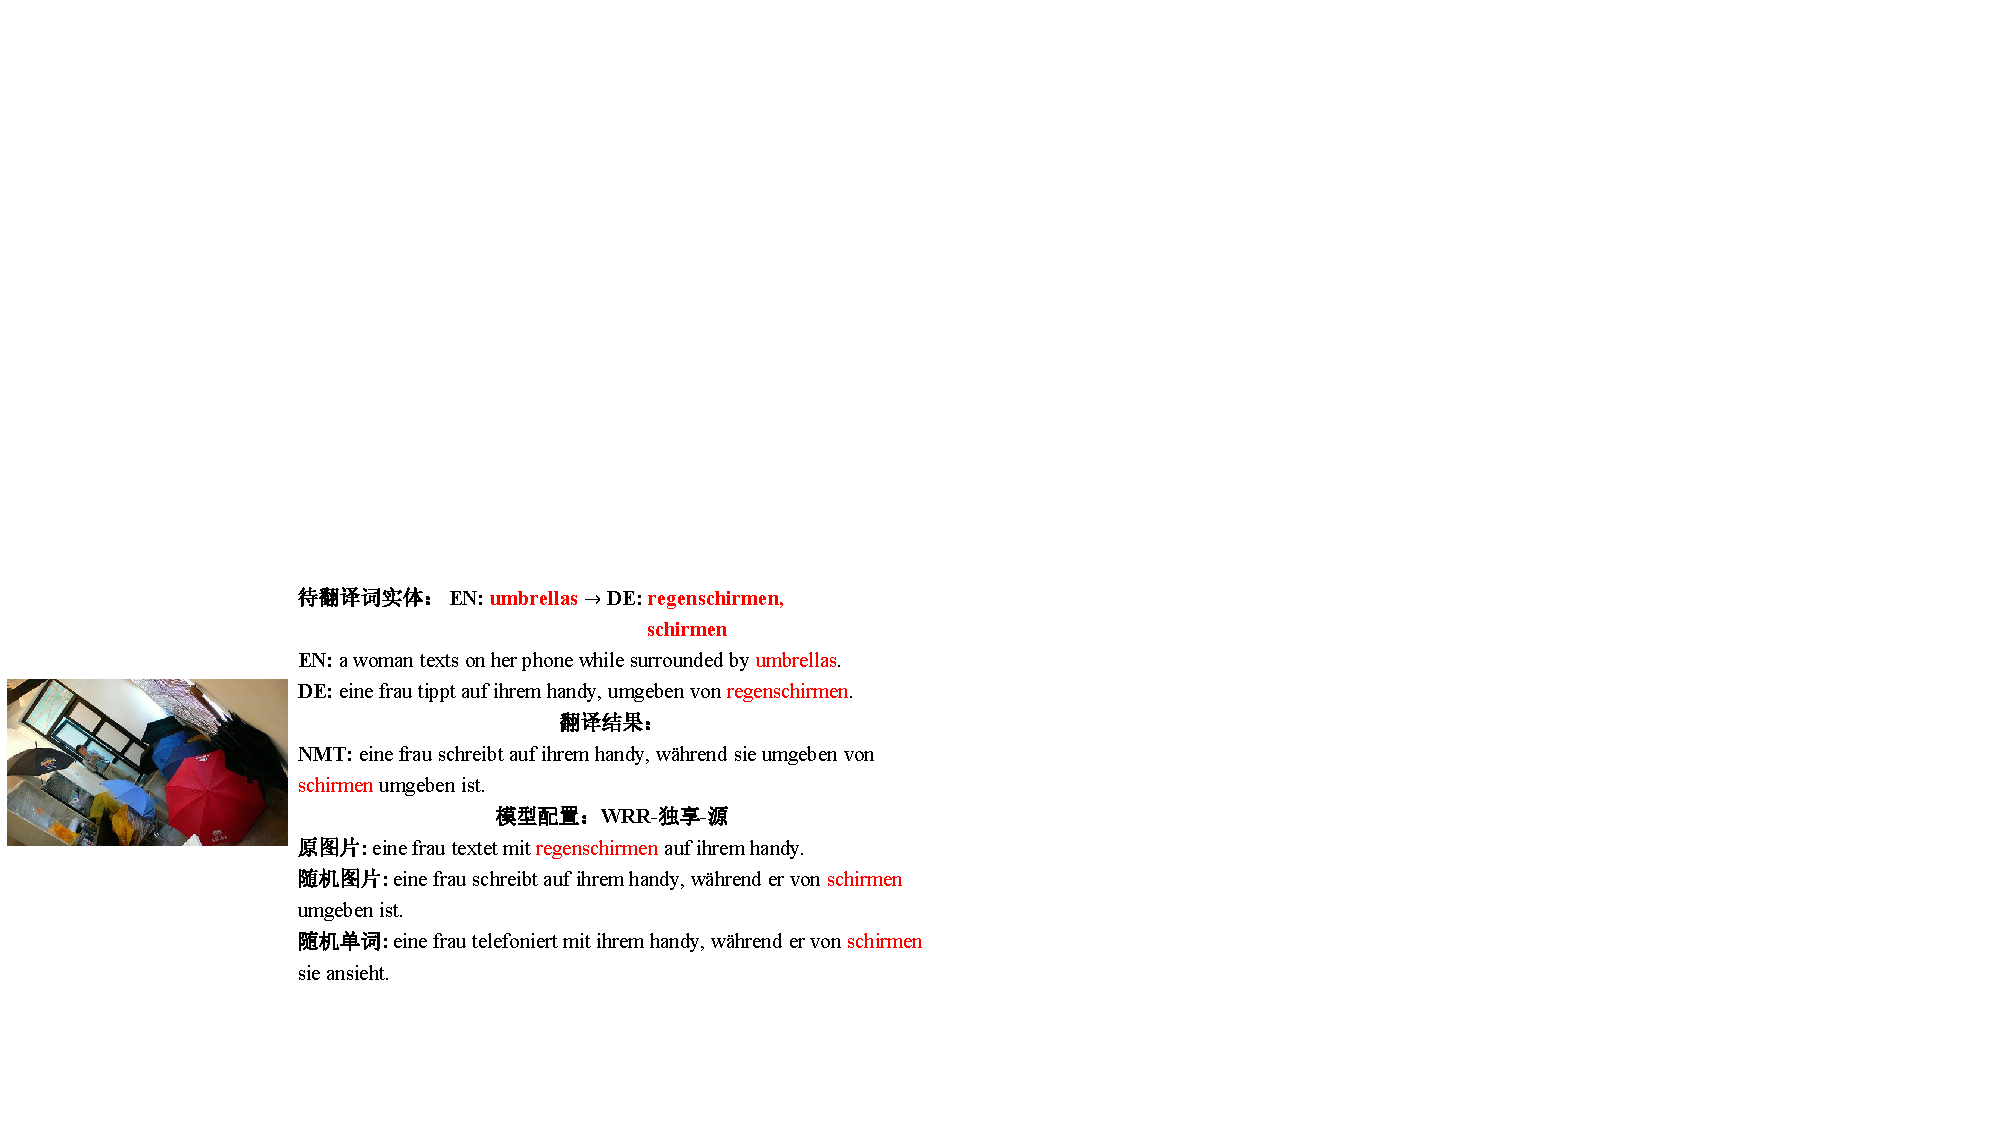
\includegraphics[scale=1.0]{Img/fig_3_case_4.pdf}
    \bicaption{实体词翻译准确率增量与增量差分析}{Accuracy increment and incremental difference analysis of entity words}
    \label{fig:3_case_4}
\end{figure}
为了展示本章所提方法对句子翻译和实体词翻译带来的影响,我们在图【】中给出了4个例子。通过观察可以得到以下结论:输入正确的图片信息时,模型的性能表现较好;当实体词有多种释义时,其它模型的翻译结果在多个释义上容易表现出不稳定的结果,本章所提方法的表现更好。

\section{本章小结}
为了探究显式跨模态信息融合方法的可行性,本章提出了一种以明确的方式将图片中的视觉目标信息与文本中对应短语或名词相融合的方法。然后将该方法应用于文本句子的重构任务,再通过参数共享的方式,将重构模型优化后的模型参数与翻译模型共享,从而增强了神经机器翻译系统的翻译性能。
该方法在融合图片信息的翻译任务常用的Multi30K英德翻译对上进行了实验,在测试阶段不需要输入图片的情况下,在基于循环神经网络的模型中取得了最佳的翻译效果,在基于Transformer的模型上与其它模型任然是可比的。
在消融与对抗训练的实验中,输入原图片的模型相比于输入随机噪声或不输入图片的掩码方案翻译性能最佳。说明文本重构模型通过利用图片信息优化了模型的参数,使翻译模型得到了增强。
在进一步的实验分析中发现,本章所提方法主要提升了实体词的翻译准确率,从而在整体上提升了译文的质量。该研究成果发表于2021年自然语言处理实证方法会议(EMNLP 2021)。

%为了探究显式跨模态信息融合的可行性,本章提出了一种以明确的方式将图片中的视觉目标信息与文本中对应的短语实体或词实体相融合的方法。并将该方法应用于文本的重构任务,最后通过多任务参数共享的方式,优化了翻译模型中对实体词的翻译能力,从而带来了进一步翻译质量的提升。实验结果表明,所提方法在测试阶段不需输入图片信息的条件下依旧与其它需要输入图片的方法是可比的,并且对词实体的翻译具有显著的提升作用。该研究成果发表于Findings of the Association for Computational Linguistics: EMNLP 2021。
\chapter{基于双向跨模态实体重构的神经机器翻译}

\section{引言}

\section{相关工作}
% 应该侧重图片重建相关的方法,大概也就3个工作(imagination,Adversarial reconstruction for Multi-modal Machine Translation,

\section{方法描述}

\section{实验设置}

\section{实验结果}

\section{本章小结}

\chapter{基于图文对比对抗训练的神经机器翻译}
% 已有工作
前两章我们聚焦于图片信息增强式的神经翻译模型,通过在模型训练阶段引入视觉信息增强模型的表示能力,从而提升纯文本翻译模型的翻译质量。
% 存在的问题
然而这种做法规避了图片信息在生成翻译过程中的辅助作用,使得视觉信息的作用没有得到充分的发挥。
% 本章所针对的问题
为此本章将主要探索图片信息辅助式的神经机器翻译方法,尝试将图片信息融入句子级别的语义信息中。在针对已有方法的讨论中我们知道,此类方法属于隐式跨模态信息融合方法,需要解决神经翻译模型对视觉信息不敏感的问题。
% 具体做法
因此,本章提出一种图文对比对抗训练方法,尝试提升视觉信息在语义表示学习过程中的参与度。在模型输入为文本加图片的情况下,通过与我们设计的图文对抗样本进行对比,使模型重视图片输入信息与文本描述之间的差异,从而将图片信息融合到文本的表示中。
% 结果
在英译德、英译日和英译印三个翻译任务上的实验表明,本章所提方法能够有效提升翻译准确率的同时,增强了模型对视觉信息的敏感度。

\section{引言}
% 大背景(跳过)
% 相关方法的做法,这里应该强调的是guide,还有就是句子级的语义融合
% 图片中往往包含了更完整更丰富的语义信息,因此为了得到更准确的翻译,在翻译过程中加入图片信息成为了一种可行的方案。为了将图片信息融合到翻译中,广大研究者付出了很多的努力。早期的相关研究尝试在句子的编码过程中输入图片使编码结果更接近真实的语义,例如将图片特征作为基于RNN的翻译模型的初始化向量【】,亦或是将图片作为一个单词输入到模型中。也有一些方法以图片特征作为语义的中枢点,尝试为来自不同语言的文字或不同模态的语义信息创造一个统一的语义空间【】。同时,也有方法尝试在解码阶段输入图片,从而引入更多可参考的信息使解码的结果更准确。例如文献【】采用了注意力机制,在基于RNN或是基于Transformer的方法中均有着相似的应用。也有方法尝试
图片中往往包含了更完整更丰富的语义信息,因此为了得到更准确的翻译,在翻译过程中加入图片信息成为了一种可行的方案。为了将图片信息融合到翻译中,广大研究者付出了很多的努力。早期的相关研究尝试在句子的编码过程中输入图片使编码结果更接近真实的语义,例如将图片特征作为基于RNN的翻译模型的初始化向量【】,亦或是作为一个单词输入到模型中。也有一些方法以图片特征作为语义的中枢点,尝试为来自不同语言的文字或不同模态的语义信息创造一个统一的语义空间【】。同时,也有方法尝试在解码阶段输入图片,从而引入更多可参考的信息使解码的结果更准确【】。这些方法普遍以句子为语义单位融合图片信息,这样做能够更充分地利用图片所包含的语义,也能最大化的优化翻译过程。

%存在问题
然而,无论是通过简单的输入或是复杂的设计,图片信息很难为翻译带来理想的效果。一方面,图片信息为翻译带来的提升是不稳定的【】;另一方面,当为待翻译句子提供与其内容不一致的图片时,对实际的翻译结果影响很小。这些问题说明一般的神经机器翻译模型对输入图片所提供的视觉信息并不敏感。

%本文做法
\begin{figure}[!htbp]
    \centering
    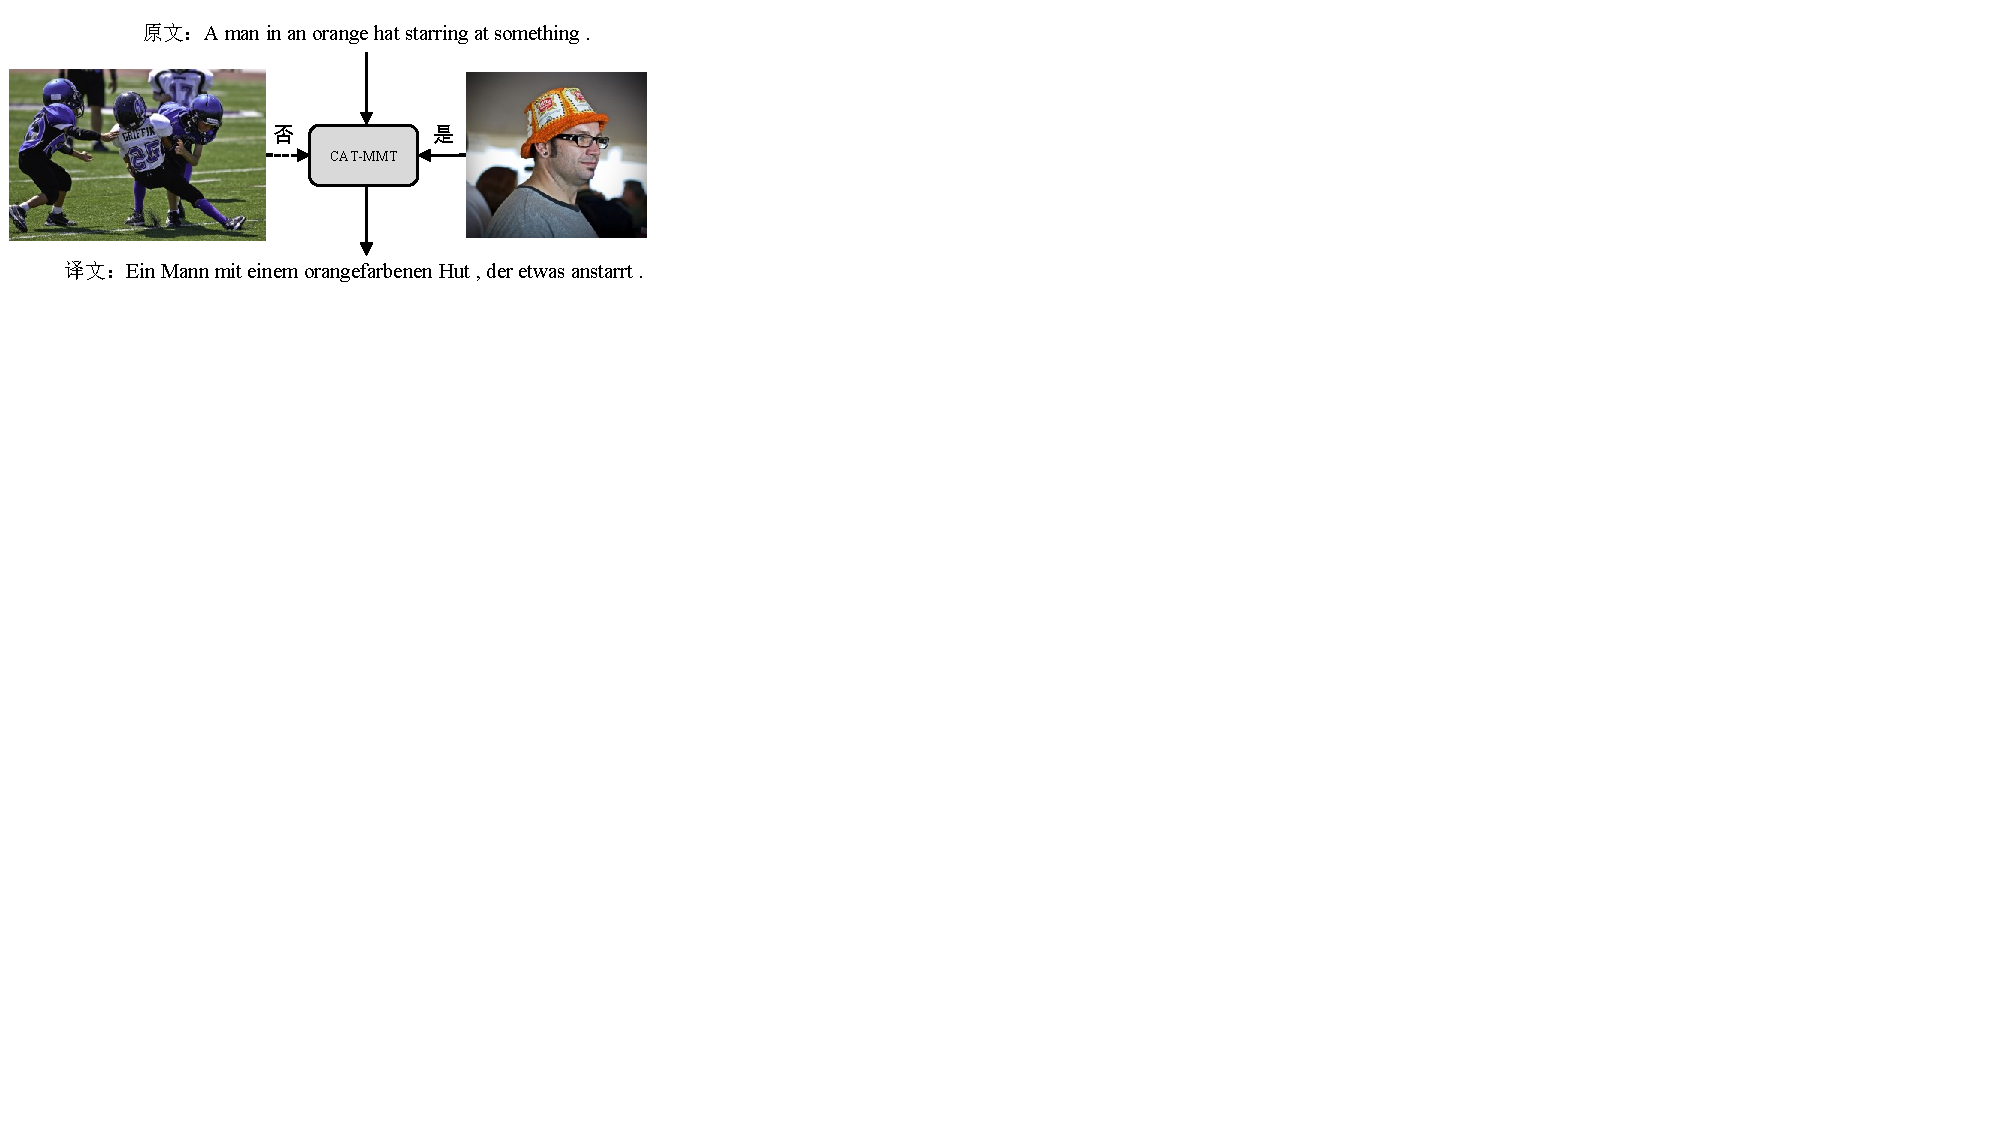
\includegraphics{Img/fig_5_example.pdf}
    \bicaption{引入对抗样本的神经机器翻译模型}{NMT model with adversarial samples}
    \label{fig:5_example}
\end{figure}
已有的相关工作表明在神经机器翻译任务中实现句子级的跨模态语义信息是很困难的。只有少部分的待翻译句子需要额外的输入图片作为信息的补充。大部分的翻译语料已经具备良好的双语对齐关系,这使得融合图片信息的端到端模型在面对更容易学习的并且是文本主导的翻译任务时,并不会过多地关注跨模态的信息对齐与融合。因此,针对神经机器翻译中的句子级跨模态语义融合方法,在讨论图片信息是否以及在哪方面能够为翻译带来质量提升之前,应该更多地关注如何让模型具备从两个模态共同获得信息的能力。为此,本章提出了一种对比对抗训练(contrastive adversarial training, CAT)方法来解决这个问题。首先,我们的模型输入与一般融合图片信息的翻译模型相似,为一个源语言句子和一张对应的图片。其中该图片中的视觉目标被提取出来,并一同输入到模型中。然后我们采用对比学习的方法来拉近输入与译文在统一语义表示空间的距离。其中,译文作为锚点(anchor),将源语言句子与对应的图片作为正样本。为了使模型关注到图片中所携带的视觉信息,我们将源语言句子与随机图片输入到模型中作为负样本。如图\ref{fig:5_example}所示,应用该策略可以强迫翻译模型关注输入的源语言文本与输入图片的语义关系,从而实现句子级别的跨模态信息融合。

%具体贡献
本章主要贡献如下:

% 主要翻译性能上的贡献
(1)本章提出了一种基于图文对比对抗训练的神经机器翻译方法,又称CAT-NMT。在配合双向翻译训练后,对比对抗训练能够有效地为融合图片信息的神经机器翻译方法带来翻译准确率的提升。该方法在三个不同的翻译数据上得到了有效的提升。

% 主要动机上的贡献
(2)本章所提方法旨在将视觉信息融合到本文的表示中,试图通过图片信息加强翻译模型在编码过程中对源语言文本的表示能力,从而提升最终翻译的质量。在对抗实验的分析中可以观察到,CAT-MMT的翻译质量提升来源于成功地将图片信息融合到了文本表示中。因此,CAT方法达到了使翻译模型对视觉信息敏感的目的。

% 分析结果的贡献
(3)在对模型结果的分析中发现,为翻译输入随机图片或不输入图片时,带有歧义词较多的测试集受到的影响最大。该结果可以表明当神经机器翻译模型对视觉信息敏感时,对文本中存在歧义词问题的句子具有更好的翻译效果。
\section{相关工作}
本章工作主要针对将加入对抗样本的对比学习方法应用到融合图片信息的神经机器翻译中,因此相关工作可以分为以下三个部分:

%传统方法:都有哪些方法,这些方法出现的问题,
{\sffamily (1)图片信息辅助式神经机器翻译}
%这里指出简单的方法,和复杂的方法
在融合图片信息的神经机器翻译方法中,将图片作为翻译模型输入的一部分,并将其用于帮助源语言文本的编码或在目标语言生成过程中提供外源参考信息的图片辅助式神经机器翻译是目前最常见的一类。图片可以以多种方式与神经翻译任务相结合,而为了更有效地利用图片信息,研究者们设计了从简单到复杂的图片信息融合方式。文献\cite{52_DBLP:journals/corr/ElliottFH15}将图片的全局特征输入到基于循环神经网络的翻译模型中,将其与源语言句子编码后的隐层向量连接后用于初始化解码器。文献\cite{18_DBLP:conf/emnlp/CalixtoL17}则尝试了更多图片全局特征的使用方法,例如直接初始化编码器,直接初始化解码器以及当做词串接到输入句子的词嵌入后。文献\cite{36_calixto-etal-2017-doubly,47_DBLP:conf/wmt/LibovickyHM18}则利用图片栅格特征可以看作图片特征序列的特性,采用注意力机制为解码器提供动态的上下文信息。这些方法均是通过简单的模型改动达到使神经机器翻译模型支持对视觉特征输入的目的。然而文献\cite{23_elliott-2018-adversarial}的对抗评估则表示以简单的方式将图片输入给模型并不能使图片信息得到很好的利用。在后续的研究进程中涌现了更多复杂的图片信息融合方法。文献\cite{39_ive-etal-2019-distilling}将图片信息作用到解码阶段后的推敲网络(deliberation network)进行二次解码。文献\cite{33_yin-etal-2020-novel}将句子与图片中的视觉目标视为图的关系,采用基于图的编码器融合跨模态信息。
然而文献\cite{53_caglayan-etal-2019-probing}的实验表明,在文本信息缺失的情况下,即便采用简单的图片输入方式,翻译模型也会更多地利用图片信息。因此,对于图片辅助式神经机器翻译方法,需要更多地关注如何使翻译模型更多地关注图片中的信息,从而加强图片信息的辅助作用。

%对比学习方法:主要有NMT的方法,MMT也有相关的概念,但与本文的不同
{\sffamily (2)基于对比学习的神经机器翻译}

对比学习方法已经广泛应用于计算机视觉和自然语言处理的相关研究中。该方法的作用是将样本空间中具有相似语义信息样本点拉近,并增加不相关样本之间的间隙。通常,相似样本之间可互称为正样本,不相关样本之间可互称为负样本。
文献\cite{70_pan-etal-2021-contrastive}在一个多语言神经机器翻译系统中加入了对比学习方法。在训练期间,每个双语翻译对都是正样本,为每对正样本从数据集中随机选取不相关句子作为负样本。在对比损失函数的配合下,针对多语言翻译的交叉熵损失函数能够帮助模型学习到多语言的统一表示空间,从而达到提升多语言之间翻译性能并帮助零资源翻译的目的。
文献\cite{80_li-etal-2021-unimo}提出了一种应用于多模态理解与生成任务的多模态预训练框架。该工作通过对比学习方法建立文本与图片之间的跨模态统一表示空间。在构建过程中,通过计算文本表示与图片表示之间的相似度,实现对来自不同模态信息的语义距离的计算。这种方式能够帮助模型获得更多的跨模态信息,从而更好地服务于下游任务。
文献\cite{37_elliott-kadar-2017-imagination}在训练纯文本的神经机器翻译模型中,引入了“想象力”机制作为翻译的子任务。该机制将文本表示映射到视觉特征的表示空间,尝试通过“想象”的方式使文本表示尽可能地接近图片中的语义。该过程就是利用了对比损失函数,使文本表示尽可能接近对应图片的特征表示,并远离同批数据下其它图片的特征表示。
文献\cite{68_DBLP:journals/corr/KirosSZ14}则是在融合图片信息的神经机器翻译中,通过建立句子与图片统一的表示空间达到应用图片信息提升文本表示的能力的目的,而在构建中同样采用了对比学习的方法。该工作在对比学习中同样加入了对抗样本作为负样本的方式,尝试拉近源语言句子与相关图片在表示空间的距离,并尝试推开与句子不相关的图片,以及推开与图片不相关句子。与该工作不同的是,本章的方法虽然也引入了对抗样本作为负样本,但并不是针对图片与文本之间语义表示的对比学习,而是将图片信息融合到文本的表示中,针对不同文本表示的对比学习,并在该过程中加入了译文作为锚点,使对比学习作用到翻译而不是跨模态表示。

%对抗训练方法:主要用于测试
{\sffamily (3)对抗训练方法}

对抗训练方法常用于在训练神经机器翻译模型时,通过引入对抗样本的方式提升系统的鲁棒性。然而,在融合图片信息的神经机器翻译中,对抗样本更多用于测试输入的图片能否在翻译的过程中起作用。
文献\cite{23_elliott-2018-adversarial}提出采用对抗评估来测试翻译模型是否利用到视觉信息。该研究在融合图片信息的神经机器翻译模型中输入与文本相对应和不对应的图片,然后通过测试模型的翻译准确率的变化来判断模型在翻译过程中是否受到输入图片信息的影响。
文献\cite{20_wu-etal-2021-good,22_li-etal-2021-vision}在分析视觉信息是否在翻译模型中起作用时,同样使用了对抗样本的方法。该工作认为图片与噪音的作用相似,是通过正则化(regularization)的方式提升了翻译模型的性能。
文献\cite{23_elliott-2018-adversarial}则采用了文本对抗输入的方式测试融合图片信息的神经机器翻译模型能否通过图片中的信息纠正对抗文本带来的错误。其结果表明图片信息无法做到纠正文本错误。这一结果也说明了虽然模型的输入同时包含了来自图片和文本两个模态的信息,但融合图片信息的神经机器翻译仍然是文本信息为主图片信息为辅的。
与以上工作在测试阶段应用对抗样本不同的是,本章所提方法将对抗样本应用于对比学习的训练过程。对抗样本作为负样本能够在对比学习的语义聚类过程中,帮助模型结合更细粒度的语义信息,从而使模型能够分辨出输入的图片信息是否与文本内容一致。
\section{方法描述}
\label{sec:5_method}

对于一个标准的图片信息辅助式神经机器翻译,其输入为一个源语言句子$X$和一个与其对应的图片$I$,然后利用这两个模态的信息生成翻译$Y$。然而,现有的很多方法对输入图片$I$中的信息并不敏感。这是因为翻译任务所使用的语料中,大部分$X$与$Y$之间有着很好的语义对齐关系。这使得翻译模型在不依靠图片输入的情况下,就可以在训练阶段学习到一组相对不错的模型参数,使模型很容易收敛到一个不需要图片信息的局部最优解。为了使模型充分利用为待翻译句子所提供的视觉信息,本章提出了基于图文对比对抗训练的神经机器翻译方法。本节将首先介绍本章所使用的翻译模型结构,然后详细介绍如何通过对比对抗训练增加模型对视觉信息的敏感度。

\subsection{模型结构}
\label{sec:5_architecture}
本章采用了一种句子级跨模态语义融合模型结构,其输入为一个文本序列,和一个可选的视觉输入,该视觉输入为文本序列所对应的完整图片以及图片内部的数个视觉目标,如图【】所示。该模型的编码器和解码器为一般的Transformer结构。其中,Transformer的编码器负责跨模态信息融合。为了使Transformer支持文本加图片形式的输入,我们采用了一个多模态嵌入层。该嵌入层共分为4个子层:词嵌入层,视觉特征层,模态分割层,位置编码层。

(1){\sffamily 词嵌入层:}为了支持图片的输入,需要在词嵌入层所对应的词表中,加入一些特殊字符:“<seg>”将词嵌入层输入的前后两部分分割为文本和视觉两个序列;“<img>”代表着放置完整图片的位置,每个输入序列仅一个;“<bbx>”代表放置图片中的视觉目标的位置,每个输入序列可以有多个;“<end>”代表着多模态输入序列的结尾。


(2){\sffamily 视觉特征层:}该层每个位置的输入与词嵌入层的特殊字符相对应,其中“<img>”的对应位置放置输入的完整图片的全局特征,“<bbx>”对应位置放置视觉目标的图片全局特征,其它位置则输入零向量。


(3){\sffamily 分割层:}这一层的作用相对简单,主要用作标识每个位置的输入属于文本序列还是图片序列。因此一共只有“文本模态”和“视觉模态”两个值,每个在模型中是一个与词嵌入层维度相同的向量。其中“<seg>”之前的文本序列均对应着“文本模态”,“<seg>”以及其后面的序列均为“视觉模态”。


(4){\sffamily 位置向量层:}这一层与一般的位置向量作用相似,能够表示输入序列中的绝对位置关系。区别在于,当输入的视觉目标与文本中的某些词有对应关系时,可以将视觉目标的位置设置为与其对应的词相同的位置,从而达到加强图片信息作用准确性的目的。如图【】所示,图片输入序列中的“帽子”的绝对位置为5,与文本序列中的“hat”保持一致。

在解码阶段,解码器仅接收“文本模态”的编码结果作为输入。这是因为本章的CAT方法旨在帮助神经机器翻译模型将视觉信息融合到文本表示中。而该过程发生在编码阶段,即没有针对解码器采取翻译以外的优化方法。因此,基于一般的翻译模型对视觉信息不敏感的假设,其内部模块,如解码器,往往也会忽略视觉信息的输入。所以,将“视觉模态”部分的隐层单元传递给解码器是多余的。

图【】中可以看到,CAT-MMT的目标函数包含了两个部分:融合图片信息的神经机器翻译所需的交叉熵损失函数和CAT所需的对比损失函数。其中交叉熵损失函数为:
\begin{equation}
    L_{CE}(\phi, \theta, \psi)=-\sum_j^M \log p(y_j|y_{<j},X,I)
\label{eq:5_cross_entropy}
\end{equation}
其中,$y_j \in Y,j=1,\cdots,M$,$\phi$为解码器参数,$\theta$为编码器参数,$\psi$为多模态嵌入层的参数。该损失函数与一般的融合图片信息的神经机器翻译模型的相似,均是通过源语言文本$X$和对应图片$I$为输入信息,生成翻译$Y$的形式。在我们的方案中,$I$代表了完整的图片与其中的多个视觉目标的组合。该损失函数无法反映出的信息是,本章的跨模态信息融合过程,仅发生在编码端。图【】中除了平均池化(average pooling)层,其它参数均需要通过翻译任务来优化。

\subsection{对比对抗训练}
\label{sec:5_cat}
正如\ref{sec:5_architecture}小节所介绍,本章是在Transformer的编码器中实现将跨模态信息融合到文本的表示中。然而,基于一般的翻译模型对视觉信息不敏感的假设,在没有额外的引导下,编码器同样会忽略图片信息的存在。为了有效地融合视觉信息,本章提出了图文对比对抗方法来实现在编码过程将图片中的视觉信息融合到文本的表示中。CAT方法主要包含三部分:对比学习,对抗样本以及双向翻译训练。

{\sffamily 对比学习}

对比学习方法能够在语义表示空间中拉近相似的样本,推离不相关的样本。针对融合图片信息神经翻译中,将目标译文$Y$作为锚点,将编码端的输入$X+I$作为正样本。在$X$与$Y$的双语统一表示空间中,对比学习方法能够拉近$X+I$与$Y$之间的距离,并将其它的所有样本视为负样本,拉开与$X+I$和$Y$之间的距离。图【】中每个圆代表文本语义表示空间的一个点,其中图【】(a)和图【】(b)展示了对比学习将表示空间的样本分簇归类的能力,图【】(b)中的每个簇可视为一个双语平行句对。常规的对比学习损失函数为:
\begin{equation}
    \mathcal{L}_{CL}(\theta, \psi)=-\log\ \frac{e^{\mathrm{sim}(\mathcal{R}(Y),\mathcal{R}(X+V))/\tau}}{\sum_{Z\in N}e^{\mathrm{sim}(\mathcal{R}(Y),\mathcal{R}(Z))/\tau}}
    \label{eq:5_contrastive_learning}
\end{equation}

其中$\mathrm{sim}(\cdot,\cdot)$为余弦相似度函数,用于计算两个表示向量的语义相似度;$\tau$为温度,控制区分正负样本的能力;$\mathcal{R}(\cdot)$代表平均池化,正如图【】所示,对比损失的输入是文本表示经平均池化后的结果;$N$代表着负样本集。

$\mathcal{L}_{CL}$与$\mathcal{L}_{CE}$之间共享编码器和嵌入层的参数,因此本章所采用的对比学习只针对编码器进行参数优化。


\section{实验设置}

\section{实验结果}

\section{本章小结}

\section{结束语与展望}

\section{工作总结}

\section{未来展望}


%-
%-> Appendix
%-
\cleardoublepage%
%\appendix% initialize the environment
%\input{Tex/Appendix}% appendix content
%-
%-> Backmatter: bibliography, glossary, index
%-
\backmatter% initialize the environment
\intotoc*{\cleardoublepage}{\bibname}% add link to toc
\artxifstreq{\artxbib}{bibtex}{% enable bibtex
    \bibliography{Biblio/ref}% bibliography
}{%
    \printbibliography% bibliography
}
%---------------------------------------------------------------------------%
%->> Backmatter
%---------------------------------------------------------------------------%
\chapter[致谢]{致\quad 谢}\chaptermark{致\quad 谢}% syntax: \chapter[目录]{标题}\chaptermark{页眉}
%\thispagestyle{noheaderstyle}% 如果需要移除当前页的页眉
%\pagestyle{noheaderstyle}% 如果需要移除整章的页眉

%此处填写致谢。


\rightline{2023年6月}
\chapter{作者简历及攻读学位期间发表的学术论文与其他相关学术成果}

%\section*{作者简历:}
%××××年××月——××××年××月,在××大学××院(系)获得学士学位。

%××××年××月——××××年××月,在××大学××院(系)获得硕士学位。

%××××年××月——××××年××月,在中国科学院××研究所(或中国科学院大学××院系)攻读博士/硕士学位。

%工作经历:

\section*{已发表(或正式接受)的学术论文:}

{
\setlist[enumerate]{}% restore default behavior
\begin{enumerate}[nosep]
    \item 第一作者. Contrastive Adversarial Training for Multi-modal Machine Translation. ACM Transactions on Asian and Low-Resource Language Information Processing (TALLIP), 2023. Accepted.
    \item 第一作者. Entity-level Cross-modal Learning Improves Multi-modal Machine Translation. In Findings of EMNLP 2021. pages 1067–1080.
    \item 第一作者. 基于跨模态实体信息融合的神经机器翻译方法.自动化学报, 2023, 49(3): 1−11
\end{enumerate}
}

\section*{申请或已获得的专利:}

1. 第二完成人。多模态机器翻译方法、装置、电子设备和存储介质。202110392717.5。

%\section*{参加的研究项目及获奖情况:}


\cleardoublepage[plain]% 让文档总是结束于偶数页,可根据需要设定页眉页脚样式,如 [noheaderstyle]
%---------------------------------------------------------------------------%
% other information
\end{document}
%---------------------------------------------------------------------------%

